%%%%%%%%%%%%%%%%%%%%%%%%%%%%%%%%%%%%%%%%%%%%%%%%%%%%%%%%%%%%%%%%%%%%%%%%%%%%%
%%%% Preamble
%%%%%%%%%%%%%%%%%%%%%%%%%%%%%%%%%%%%%%%%%%%%%%%%%%%%%%%%%%%%%%%%%%%%%%%%%%%%%

%%%% The uwthesis.sty file relies on the memoir class!
%%%% You should be using the memoir class anyway; it makes life easier:
%%%% http://www.ctan.org/tex-archive/macros/latex/contrib/memoir/

%\begin{Huge}
%\begin{huge}
%\begin{LARGE}
%\begin{Large}
%\begin{large}
%\begin{normalsize} % (default)
%\begin{small}
%\begin{footnotesize}
%\begin{scriptsize}
%\begin{tiny}

\newcommand{\pp}{\Pp\Pp\xspace}
\newcommand{\PH}{\ensuremath{H}}
\newcommand{\PZ}{\ensuremath{Z}}
\newcommand{\PW}{\ensuremath{W}}
\newcommand{\Pgg}{\ensuremath{\gamma}}
\newcommand{\cPg}{\ensuremath{g}}
\newcommand{\Pgt}{\ensuremath{\tau}}
\newcommand{\tauh}{\ensuremath{\tau_{h}}}
\newcommand{\Pgm}{\ensuremath{\mu}}
\newcommand{\Pe}{\ensuremath{e}}
\newcommand{\PGpz}{\ensuremath{\pi^{0}}}
\newcommand{\Pp}{\ensuremath{p}}
\newcommand{\pt}{\ensuremath{p_\mathrm{T}}}
\newcommand{\kt}{\ensuremath{k_\mathrm{T}}}
\newcommand{\PT}{\ensuremath{P_\mathrm{T}}}
\newcommand{\TeV}{\ensuremath{\mathrm{TeV}}\xspace}
\newcommand{\GeV}{\ensuremath{\mathrm{GeV}}\xspace}
\newcommand{\NA}{\textsc{N/A}}
\newcommand{\stat}{\ensuremath{(stat.)}}
\newcommand{\syst}{\ensuremath{(syst.)}}
\newcommand{\thy}{\ensuremath{(theory)}}
\newcommand{\ttbar}{\ensuremath{t\bar{t}}\xspace}
\newcommand{\bbbar}{\ensuremath{b\bar{b}}\xspace}
\newcommand{\fbinv}{\ensuremath{f^{-1}}\xspace}
\newcommand{\MT}{\ensuremath{m_\mathrm{T}}}
\newcommand{\mvis}{\ensuremath{m_\text{vis}}}
\newcommand{\mtt}{\ensuremath{m_{\Pgt\Pgt}}}
\newcommand{\hww}{\ensuremath{\PH\to\PW\PW}}
\newcommand{\htt}{\ensuremath{\PH\to\Pgt\Pgt}}
\newcommand{\pth}{\ensuremath{\pt^{\tau\tau}}}
\newcommand{\mjj}{\ensuremath{m_\mathrm{jj}}}
\newcommand{\aMCATNLO}{\textsc{aMC@NLO}\xspace}
\newcommand{\POWHEG}{\textsc{POWHEG}\xspace}
\newcommand{\PYTHIA}{\textsc{PYTHIA}\xspace}
\newcommand{\HERWIG}{\textsc{HERWIG}\xspace}
\newcommand{\FASTJET}{\textsc{FASTJET}\xspace}
\newcommand{\emu}{\ensuremath{\Pe\Pgm}}
\newcommand{\etvecmiss}{\ensuremath{\vec{E}^{miss}_T}}
\newcommand{\MET}{\ensuremath{\etvecmiss}}
\newlength\cmsTabSkip
\setlength\cmsTabSkip{1.6ex}
\newcommand{\ptmiss}{\ensuremath{\pt^\text{miss}}}
\newcommand{\ptvec}{\ensuremath{\vec{\pt}}}
\providecommand{\mH}{\ensuremath{m_{\PH}}}

\documentclass[oneside, letterpaper, 12pt, oldfontcommands]{memoir}

\setsecnumdepth{subsection}

%%%% Import uwthesis.sty to get official formatting, then set your variables.
\usepackage{uwthesis}
\usepackage{mathtools}
\usepackage{xspace}
\usepackage{lineno}
\linenumbers
%\usepackage{amsmath}
\DeclarePairedDelimiter{\abs}{\lvert}{\rvert}

\settitle{A Study of the Standard Model Higgs Boson Decaying to a Pair of Tau Leptons at the CMS Detector}
\setauthor{Tyler Ruggles}
\setdepartment{Physics}
\doctors % or \masters
\setgraddate{2018}
\setdefensedate{15 May 2018} % or whatever format you want

%%%% Members of the Final Oral Committee (FOC)
%%%% Give name, rank, and department
%%%% 
\setfoca{Sridhara Dasu}{Professor}{Physics} % <- Your advisor
\setfocb{Wesley H Smith}{Professor}{Physics}
\setfocc{Matthew F Herndon}{Professor}{Physics}
\setfocd{TBA}{Professor}{Physics}
\setfoce{TBD}{Professor}{Not Physics}


%%%% Your abstract, used for the UMI abstract and in your front matter
\setabstract{%
  An analysis of the Standard Model Higgs Boson observed decaying to 
  tau leptons. The analysis utilizes the full 2016 data set collected
  by the CMS experiment.
}

%%%%%%%%%%%%%%%%%%%%%%%%%%%%%%%%%%%%%%%%%%%%%%%%%%%%%%%%%%%%%%%%%%%%%%%%%%%%%
%%%% Document
%%%%%%%%%%%%%%%%%%%%%%%%%%%%%%%%%%%%%%%%%%%%%%%%%%%%%%%%%%%%%%%%%%%%%%%%%%%%%

\begin{document}

% Tell the memoir class to set up lowercase roman for pagination, etc.
\frontmatter

%%%% Uncomment this to create a UMI abstract page.
%%%% If you are submitting electronically, however, this page is unnecessary.
% \theumiabstract

% The title page
\thetitlepage
\clearpage

% The copyright page, if you want to pay the fee and register copyright.
\thecopyrightpage
\cleardoublepage

% These above pages should not be counted, so we reset the counter to 1.
\setcounter{page}{1}

% An abstract may be required by your department.
\section{Abstract}
\uwabstract
\cleardoublepage

% Acknowledgements go here if you want to include them.
\section{Acknowledgements}
This is where any acknowledgements would go.
\clearpage

% Table of contents
\maxtocdepth{subsection}
\tableofcontents* % the * means that there isn't an entry for the TOC itself
% \clearpage
% \listoffigures  % if you have any figures
% \clearpage
% \listoftables   % if you have any tables

% Tell the memoir class to set up normal pagination, etc. for the main doc
\mainmatter

%\chapter{Introduction}
\label{sec:introduction}

This thesis presents the first observation of the Higgs boson decaying to a pair
of tau leptons ($\Pgt^{+}\Pgt^{-}$) at 13\TeV. It includes two analyses which target different
ways the Higgs boson is produced. The analyses are performed using
13\TeV center-of-mass energy proton-proton collision data from the CERN LHC.
The data is collected by the CMS experiment and corresponds to an integrated
luminosity of 35.9\fbinv. The results here constitutes an important
milestone in the effort to better understand the fundamental properties of nature and
the Higgs boson, one of the fundamental particles of the standard model (SM) of physics.

The standard model of physics is a mathematical framework for explaining
the interactions and behavior of the fundamental particles observed in nature.
It has been built up and defined through the 1950s and 60s culminating in the
theoretical prediction of the existence of a neutral scalar boson, now called the
Higgs boson.
The SM incorporates descriptions of three of the four fundamental forces of nature:
the strong force, the electromagnetic force, and the weak force.
The gravitational force is the one fundamental force not described in the SM. 

The Higgs boson eluded observation by experimental particle physicists
for 40 years after the establishment of its theoretical prediction. 
In 2012, the Higgs boson was discovered 
by the CMS and ATLAS collaborations at CERN~\cite{Aad:2012tfa, Chatrchyan:2012xdj, Chatrchyan:2013lba}.
With this discovery, all particles predicted and described in the SM have been observed.
Based on research leading up to today, the SM is the most well tested theory of nature at the fundamental level.
Over all, the SM shows remarkable consistency between theoretical predictions and
the resulting experimental observations.

Reflecting on the discovery of the Higgs boson, the focus of the experimental particle physics community has transitioned from
Higgs boson ``discovery'' mode to Higgs boson ``measurement'' mode. High energy particle physics experiments
are dedicating a vast portion of their research effort and person power towards
efforts to measure the Higgs boson properties as precisely as possible. Many 
of of these properties are firmly predicted by theory. Affirmation or negation of these predictions,
such as how often a Higgs boson decays into a pair of $\Pgt$ leptons,
are critical to further testing the merits of the SM. Affirmation of the
predicted Higgs boson properties would further support the SM along with the myriad previous
experimental results. Significant discrepancies between the SM
theoretical predictions and the observed Higgs boson properties could point to
flaws in the SM and would lead to a more full and complete understanding of nature.

This thesis is arranged to build up a theoretical understand of the SM and the
Higgs boson in Chapter~\ref{sec:pheno}. A description of the LHC machine and
CMS detector follow in Chapter~\ref{sec:cms_lhc}. The next two Chapters, ~\ref{sec:simulation} and
~\ref{sec:obj_reconstruction}, discuss the foundations of physics analyses at CMS including physics
simulations and details of how detector information is processed to reconstruct $\Pgt$
leptons and other particles. Chapter~\ref{sec:htt_analysis} covers the analysis
of the Higgs boson when produced via the gluon fusion or vector boson fusion
processes and Chapter~\ref{sec:vh_analysis} covers the Higgs boson associated
production processes. In Chapter~\ref{sec:cmb_results}, the results of
both analysis are combined together to achieve the most robust 13\TeV Higgs
boson decaying to $\Pgt^{+}\Pgt^{-}$ results possible. Finally, the thesis
is drawn to a conclusion in Chapter~\ref{sec:conclusion}.

The Higgs boson decay process to a pair of $\Pgt$ leptons will be denoted
$\htt$ through out this thesis where the $\pm$ are dropped from the $\Pgt$ superscript
for convenience.
The rest of this chapter introduces the particles and forces of the SM as well
as previous experimental results. For a more detailed mathematical treatment
of the phenomenology of SM see the following Chapter~\ref{sec:pheno}.


\section{The Standard Model of Particle Physics}
The standard model of particle physics~\cite{Glashow:1961tr,SM1,SM3} is currently
the best mathematical framework for predictions and explanations of the behavior
of the fundamental particles of nature. Fundamental particles can be grouped
together by behavior and common characteristics and arranged diagrammatically as in
Figure~\ref{fig:sm_particles}. The particles are split vertically into two categories:
fermions which have spin $\frac{1}{2}$, and the bosons which have integer
spin of either 0 or 1. In general, the fermions constitute what we are familiar of
as matter while bosons are the mediators of the fundamental forces.

\begin{figure*}[htbp]
\centering
     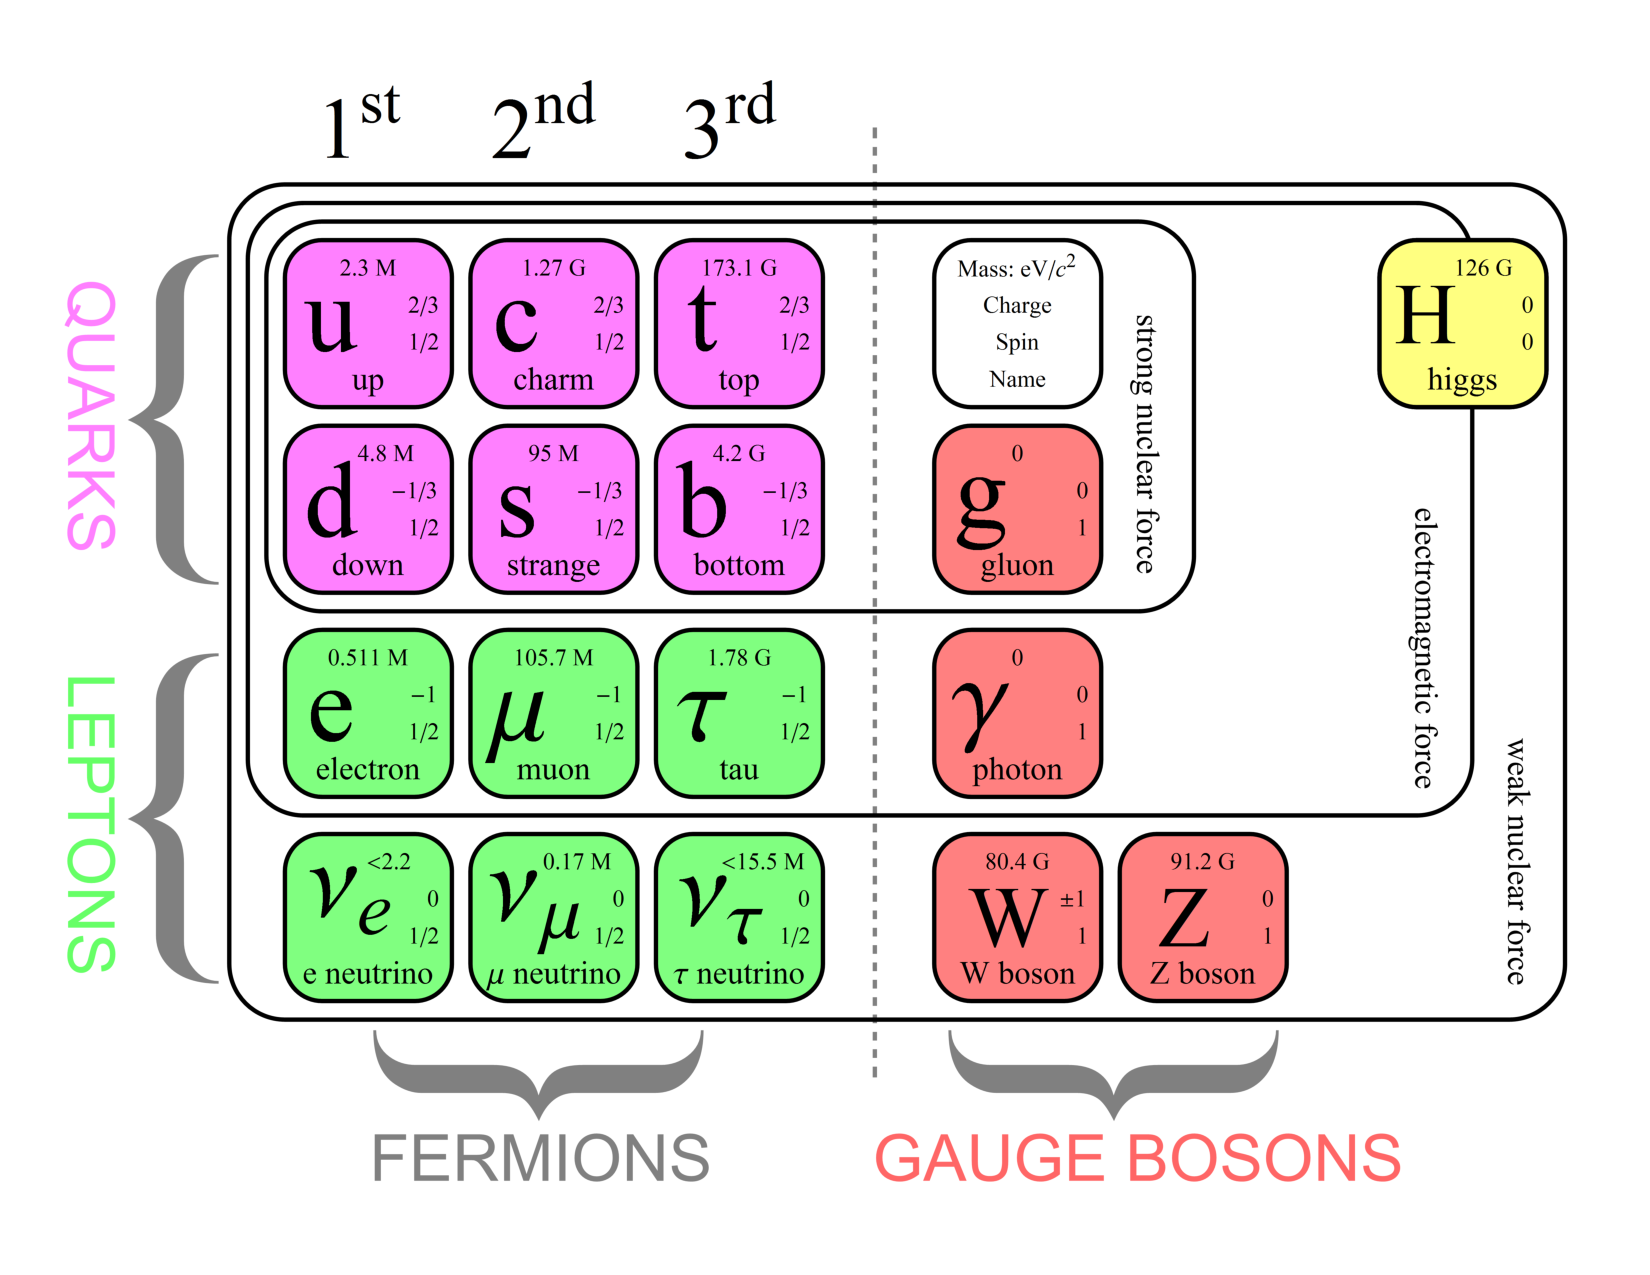
\includegraphics[width=0.7\textwidth]{introduction/plots/sm_particles.pdf}
     \caption{
The fundamental particles of the SM and some of their properties including their:
mass, electric charge, and spin. The units for mass are reported as electron volts divided by
the speed of light ($c$) squared and use scientific notation prefixes.
M for million, G for billion.
     }
     \label{fig:sm_particles}
\end{figure*}

The fermions can be further grouped into either quarks or leptons based on whether
they carry ``color'' charge or not. 
Quarks carry a color charge and have a fractional electric charge of either $-\frac{1}{3}e$ or $\frac{2}{3}e$
where $e$ is the elementary charge ($1.602 \times 10^{-19}$ Coulombs).
Where as the leptons are colorless (carry no color charge) and
have integer electric charge of 0$e$ or -1$e$. In Figure~\ref{fig:sm_particles} the fermions are
arranged according to what is called their mass ``generation'' with more massive
particles appearing to the right in the third mass generation column.

The first
mass generation column composes the fundamental particles which make up the ordinary matter
interact with every day. Up-quarks and down-quarks are the fundamental constituents within
protons and neutrons which build the atoms and molecules
making up the paper pages of this thesis or the metals and plastics in your computer. High energy protons
have a different composition and are discussed later in the thesis. Electrons are the
remaining fundamental particles we are familiar with and are also part of the basic 
structure of atoms. The electron neutrino is less familiar because it only
interacts with the other particles through the weak force and does not directly
contribute to the basic atoms.

The bosons are split into two groups, the gauge bosons which mediate the three fundamental
forces of the SM, and the solo Higgs boson which behaves differently
and will be discussed in the following chapter. 
The fundamental forces, their mediator particles, and the relative strength of that force
are listed in Table~\ref{tab:sm_forces}. The relatively weak strength of the gravitational
force is what allows the SM to still successfully predict the behavior
of particles despite not including the gravitational force.

\begin{table*}[htbp]
\centering
\begin{tabular}{lcc}
Fundamental Force        &    Force Mediator             & Relative Strength   \\
\hline
Strong                   &    gluon ($\Pg$)              &   1                 \\ 
Electromagnetic          &    photon ($\Pgg$)            &   $10^{-3}$         \\ 
Weak                     &    $\PW$ and $\PZ$ bosons     &   $10^{-14}$        \\ 
Gravitational            &    unknown                    &   $10^{-43}$        \\ 
\hline
\end{tabular}
\caption{
The fundamental forces, their mediator particles, and the relative strength of the force.
There has been no observed mediator for the gravitational force.
}
\label{tab:sm_forces}
\end{table*}

The strong force has the largest relative strength of the fundamental forces but
the reach, or distance over which the force can be felt, is very limited and is 
confined to the sub-atomic scale, $10^{-15}$m. The strong force is experienced
between particles with a color charge, exclusively gluons and quarks.
Figure~\ref{fig:sm_forces} shows a diagram of the SM particles with
lines linking force mediating bosons with the particles which experience that force.
For example, a line links the quarks with the gluons representing the
strong force.

The electromagnetic force follows after the strong force in order of largest relative
strength. The reach of the electromagnetic force is infinite and decreases with
distance as $\frac{1}{r^{2}}$. Despite its infinite reach, the electromagnetic 
force is not experienced on the macroscopic scale because stable matter is composed
of equal portions positively charged and negatively charged matter. This leads to
an overall neutral electrical charge for the universe. The electromagnetic force is experienced by all
electrically charged particles: quarks, the charged leptons, and the $\PW^{\pm}$ bosons.
This force is mediated by the photon which has neutral electric charged.
% XXX Add example of electrons holding you up in your chair, preventing you from
% falling through it?

The next force in descending order of relative strength is the weak force.
The weak force is experienced by
all of the leptons and the quarks and is mediated by the $\PW^{\pm}$ and $\PZ$ 
bosons. It is responsible for familiar phenomena such as the radioactive decay of atoms. 
Beta decay is one example of radioactive decay where, within an atomic nucleus,
a neutron is transformed into a proton and an electron and an electron antineutrino
(more on antiparticles following). Fundamentally, what happens
is the quark composition within the proton changes thereby changing the proton to a
neutron. This process is mediated by a $\PW^{-}$ boson which subsequently decays
to an electron and the antielectron neutrino.

The final and weakest force is the one we are most familiar with, the gravitational
force. Just like the electromagnetic force, the reach of the gravitational force 
is infinite and decreases with distance as $\frac{1}{r^{2}}$. Yet, unlike the
electromagnetic force, gravity is felt over extremely large distances. This is because
gravity is a purely attractive force which acts on all massive particles.
The force we are most colloquially familiar with is actually the
weakest of the four fundamental forces. Because the gravitational force is so weak
when talking about the effect on a single particle, it can be ignored for
all of the particle physics calculations throughout this thesis.

\begin{figure*}[htbp]
\centering
     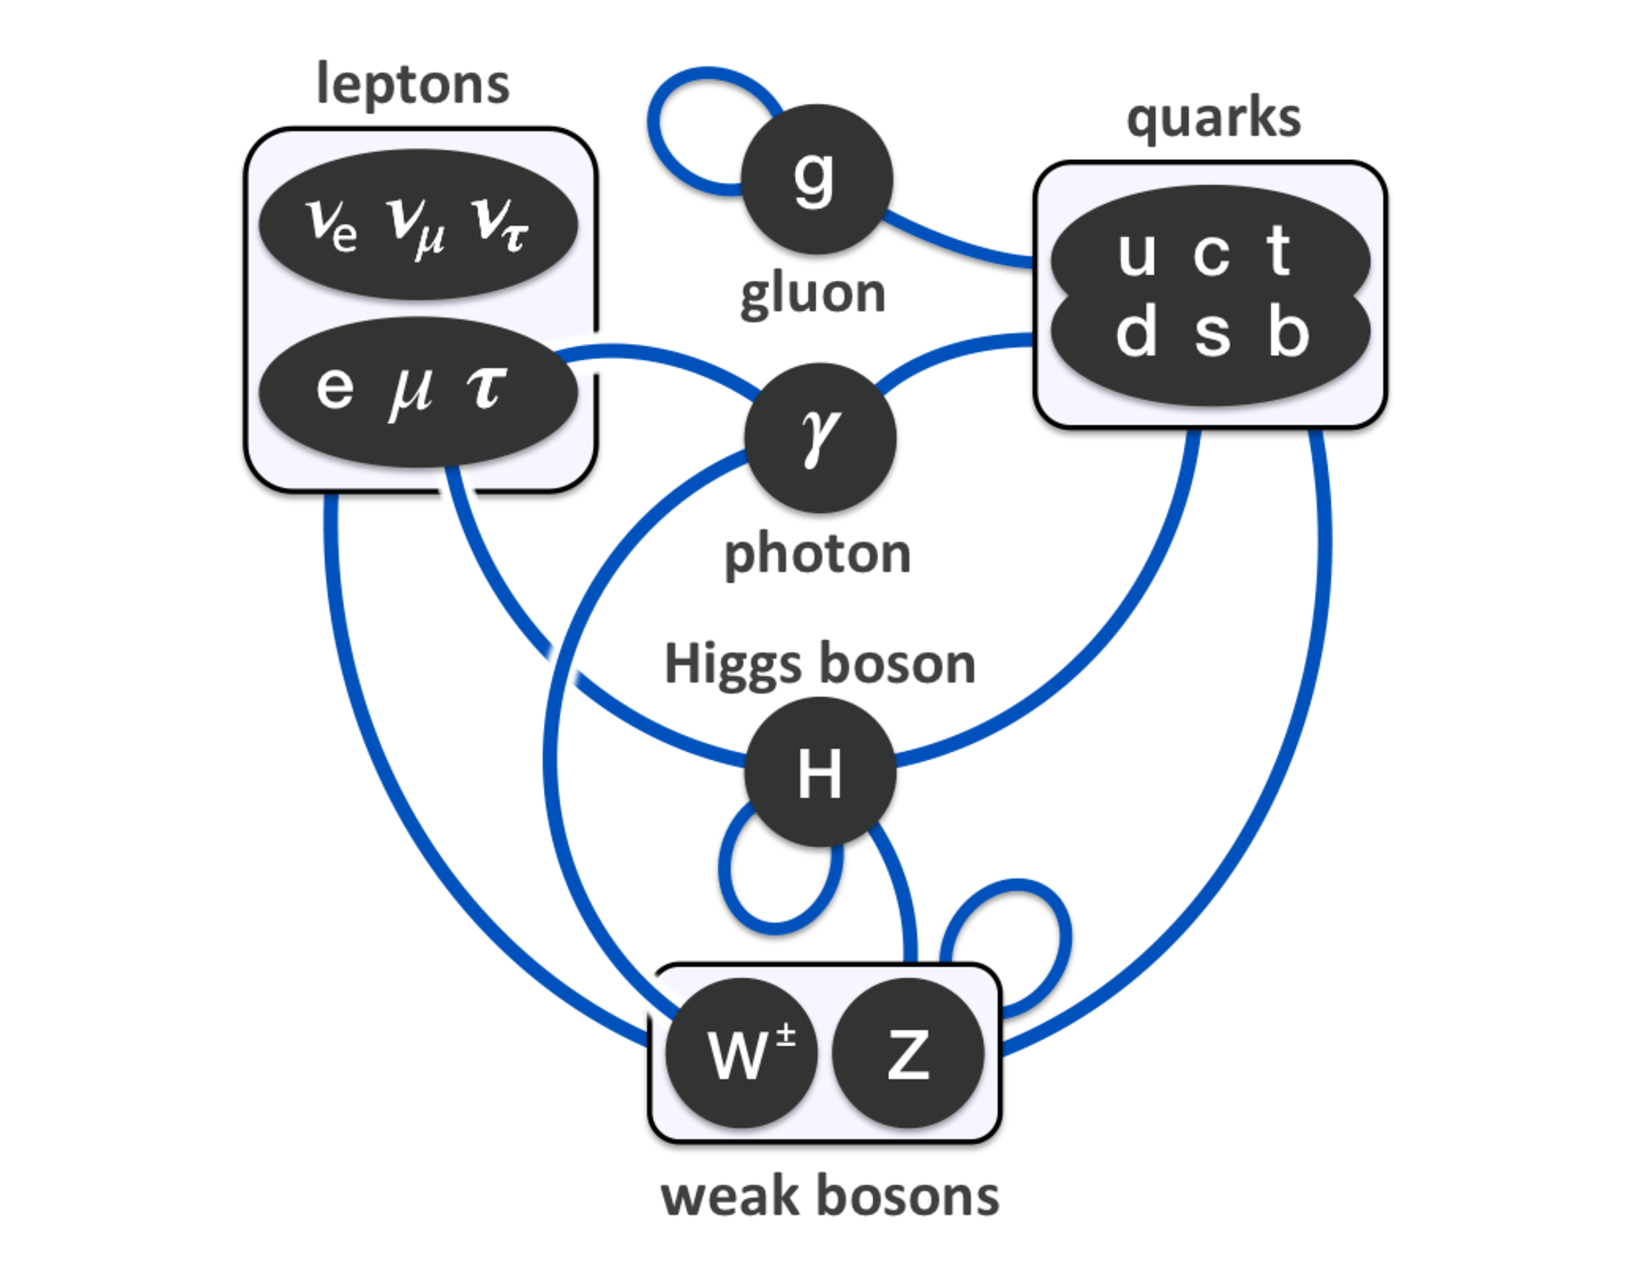
\includegraphics[width=0.7\textwidth]{introduction/plots/elementary_particle_interactions_SM.pdf}
     \caption{
Diagram showing the bosons arranged into a central column with the fermions in the
upper corners. The blue lines linking particles and groups of particles together
indicate that those fermions can be influenced by force associated to that mediator
boson. The Higgs boson in the center is discussed in Chapter~\ref{sec:pheno}.
     }
     \label{fig:sm_forces}
\end{figure*}

In addition to the particles shown in Figure~\ref{fig:sm_particles}, there exist antiparticles
which were mentioned previously in regard to beta decay.
Each SM particle has an antiparticle, though some particles, such as the photon
are their own antiparticle. Antiparticles have the same mass as their
``normal'' particle pair except they have opposite electric charge. The antiparticle
partner of the electron is the positron which is sometimes called an antielectron.
Antiparticles can be created in many types of interactions in particle physics experiments
and are relatively common. One characteristic of antiparticles is that when a particle and its 
corresponding antiparticle are in close proximity they can annihilate each other resulting in
a burst of energy.
Antiparticles are denoted in this thesis with a ``bar'' over the top of a particle symbol. For example
a top-quark is $t$ while an antitop-quark is $\bar{t}$.

For a more thorough treatment of the SM, its particles, and its forces see
Chapter~\ref{sec:pheno}.



\section{The Standard Model: Experimental Context}
The gap between the prediction of the Higgs boson and its discovery was a long 40 years.
Many of the particles making up the SM were not discovered when the Higgs boson
was originally being theorized. In fact, the existence of quarks or the discovery 
of gluons, the mediator of the strong force, were still to happen. The same is true
for the $\PW$ and the $\PZ$ bosons, the mediators of the weak force. The decades after the
1960s saw discovery after discovery, slowly piecing together and validating
the SM.

The internal structure of protons was illuminated by
deep inelastic scattering experiments carried out at SLAC which eventually led to 
the observation of the three least massive quarks: up ($u$), down ($d$), and strange ($s$)
in 1969~\cite{PhysRevLett.23.930,Breidenbach:1969kd}. In 1974, the $J/\Psi$ particle, a composite 
particle made from a charm quark ($c$) and a charm anti-quark ($\bar{c}$) was 
discovered~\cite{PhysRevLett.33.1404,PhysRevLett.33.1406}. 
The bottom quark ($b$) was discovered in 1977 via the decays of a new particle, the Upsilon
meson~\cite{PhysRevLett.39.252}. The top quark ($t$) was the last quark of the three
known generations discovered
and was not found until 1995 at Fermilab~\cite{PhysRevLett.74.2626,PhysRevLett.74.2632}.
The gluon which mediates the strong force for all of the quarks was discovered in 
1979 at DESY~\cite{PhysRevLett.43.830}.

Beyond the partons, physicists made discoveries of new bosons, specifically the mediators
of the weak force.
In 1983 the $\PW$ and the $\PZ$ bosons were discovered~\cite{AUBERT1983275,1983398}. 
These two bosons were the
most massive fundamental particles at the time of their discovery with masses of
84.4\GeV and 91.2\GeV, respectively.
A very important discovery laying the foundation for the analyses in this thesis is
the discovery of the third generation $\Pgt$ lepton, which was discovered
in 1975 by Martin Perl~\cite{PhysRevLett.35.1489}. While far from an exhaustive list,
these many discoveries give an indication of the strong background of experimental
research supporting the SM.

\section{Higgs Boson: Experimental Results}
As more pieces of the SM fell into place and particle accelerators became more powerful,
searches for the Higgs boson were conducted at multiple experiments such as the searches
at the LEP at CERN in the 1990s~\cite{Barate:2000ts,Abdallah:2003ip,Achard:2001pj,Abbiendi:2000ac}.
In the datasets corresponding to these searches, there were few enough potential Higgs
boson events that no discoveries could be made.
Instead, these searches all resulted in placing limits on the possible mass and cross section
of the Higgs boson. The Tevatron at Fermilab was active in Higgs boson searches through the early 2000s
with multiple analyses targeting the same decay process studied in this thesis, $\htt$. 
Similar to the LEP results, these analyses
placed limits on the possible mass and cross section of the Higgs boson~\cite{Aaltonen:2012jh, Abazov:2012zj}.

The discovery of the Higgs boson required higher collision energies than those provided
by the Tevatron, which reached a maximum center-of-mass collision energy of 1.96\TeV. The
LHC at CERN was designed to deliver this increase in collision energy and in 2010 the LHC started
delivering proton-proton collisions at up to 7\TeV; an increase to 8\TeV followed in 2012.
Using the proton-proton collision data with center-of-mass energy 7 and 8\TeV,
a particle compatible with the Higgs boson expectations was observed by the CMS and ATLAS experiments at the CERN LHC
in events where the Higgs boson decays to $\PZ\PZ$, $\Pgg\Pgg$, and 
$\PW\PW$~\cite{Aad:2012tfa, Chatrchyan:2012xdj, Chatrchyan:2013lba}.

Using this same set of data, other analysts pursued the $\htt$ decay process and
the CMS Collaboration showed evidence for the $\htt$ process with an observed
significance of 3.2 based on an expected significance of 3.7 standard deviations (s.d.)
for a Higgs boson mass of 125\GeV~\cite{Chatrchyan:2014nva}.
The ATLAS experiment reported evidence for the $\htt$ process 
with an observed (expected) significance of 4.5\,(3.4)
s.d. for a Higgs boson mass of 125\GeV~\cite{Aad:2015vsa}.
The combination of results from both experiments yields an observed (expected)
significance of 5.5\,(5.0) s.d.~\cite{Khachatryan:2016vau}.

Further analysis from both experiments, described in References~\cite{Aad:2015gba, Khachatryan:2014jba, 
Chatrchyan:2012jja, Aad:2013xqa, Khachatryan:2014kca,Sirunyan:2017exp},
established that the measured properties of the new particle,
including its spin, charge-parity properties, and coupling strengths to SM particles, 
are consistent with those expected for the Higgs boson predicted by the SM.
The mass of the Higgs boson ($\mH$) has been determined to be
$125.09\pm0.21\stat\pm0.11\syst\GeV$, from a combination of
ATLAS and CMS measurements~\cite{Aad:2015zhl}. An example of these measurements
can be seen in Figure~\ref{fig:run_1_comb_mu} which shows the best fit value for the signal
strength for the Higgs boson production and decay processes. As can be seen, the
majority of the $\Pgt\Pgt$ decay process measurements shows agreement with the SM predictions for the Higgs
boson. The measurements corresponding to $\htt$ with the Higgs bosons produced in association
with a $\PW$ boson ($\PW\PH$) and the measurement of the Higgs boson produced with
two top-quarks ($\ttbar\PH$) show some deviation from the SM prediction. However, 
the uncertainties are sizable and are represented by the size of the 1$\sigma$ band. Further data collection and analysis
will reduce the size of the 1$\sigma$ uncertainty band and will show if 
these deviations are statistically significant or if they are 
temporary fluctuations that are smoothed out with more data collection.

\begin{figure*}[htbp]
\centering
     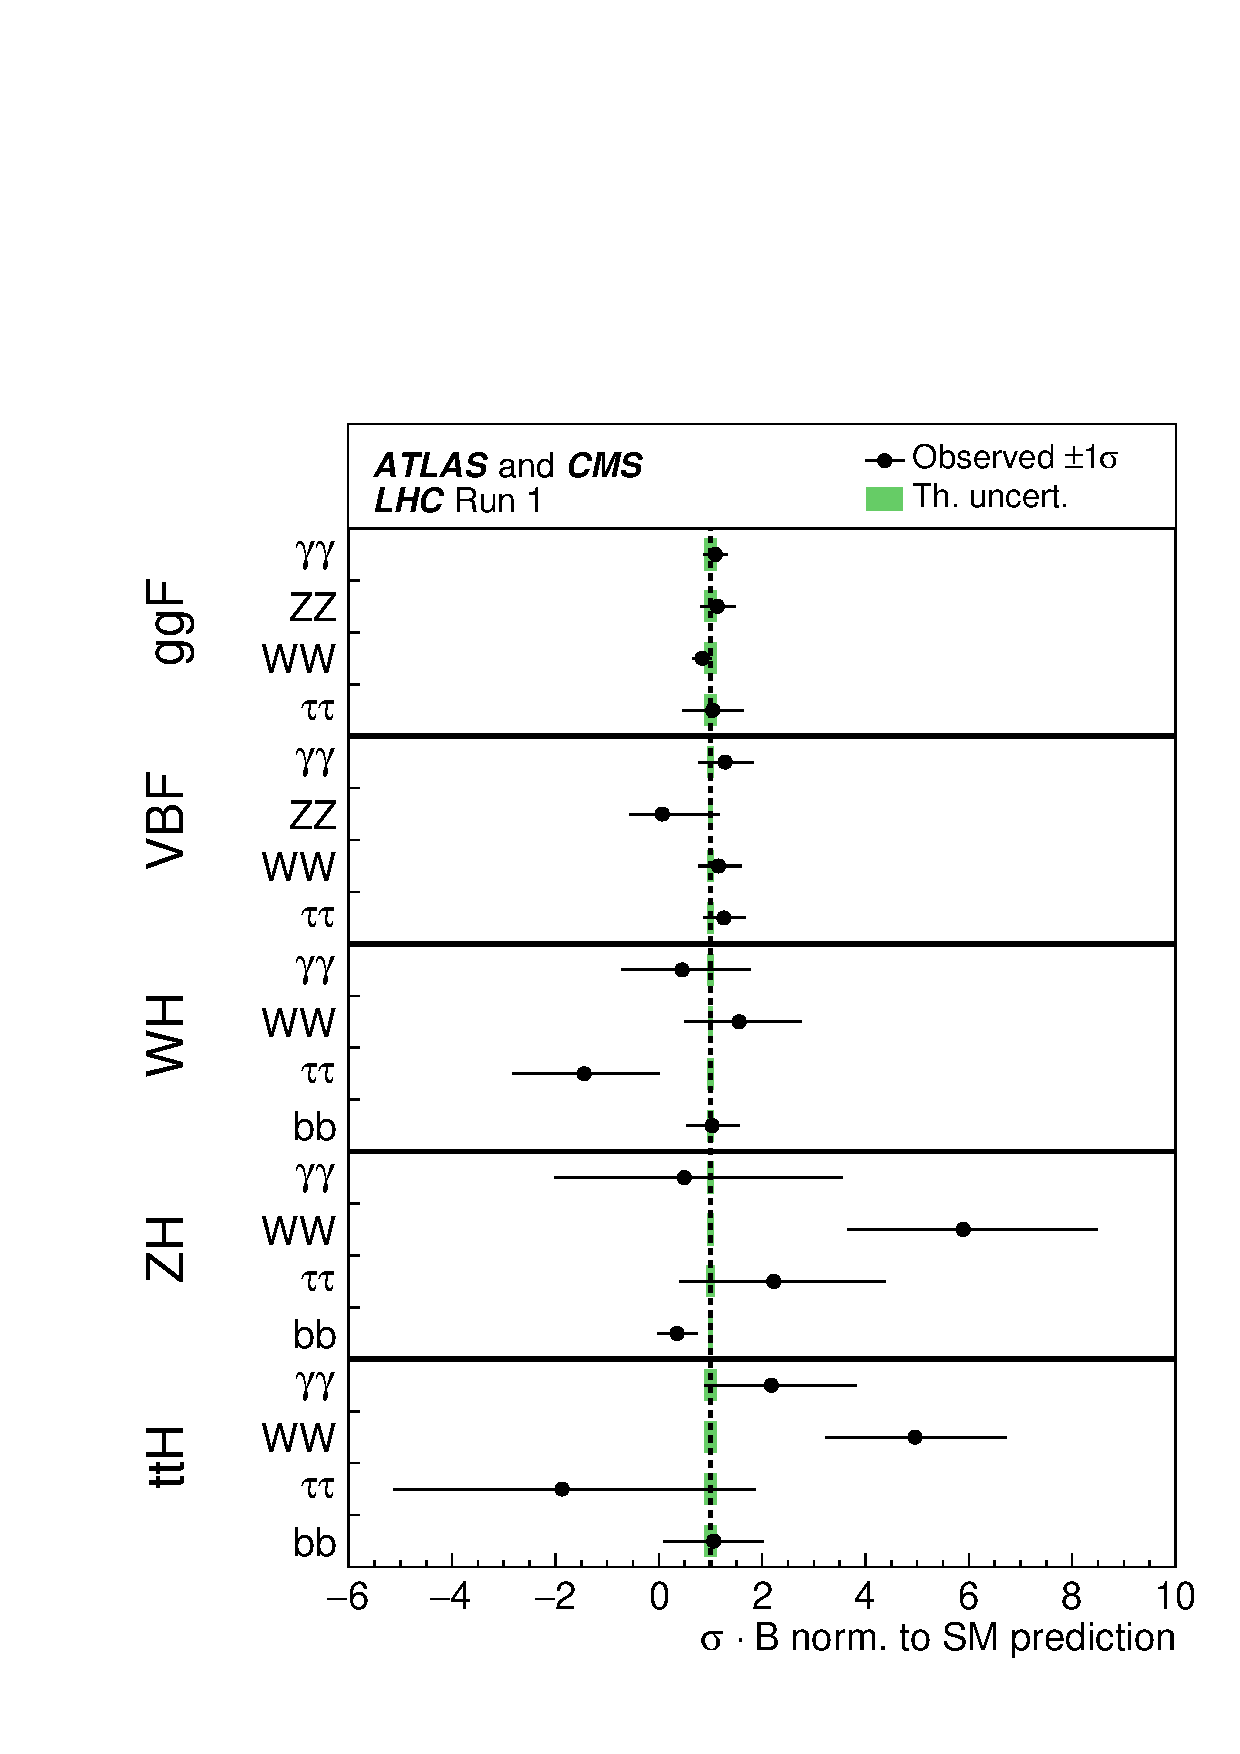
\includegraphics[width=0.6\textwidth]{introduction/plots/run_1_comb_mu.pdf}
     \caption{
The best fit values for the signal strength of the listed Higgs boson production
processes and decay processes. A value of 1 indicates perfect agreement with the SM.
The error bars indicate the 1$\sigma$ intervals. The green shaded bands indicate the
theoretical uncertainties in the predictions.
     }
     \label{fig:run_1_comb_mu}
\end{figure*}

This thesis builds on these previous experimental results at 7 and 8\TeV and measures the
properties of the Higgs boson in the $\htt$ decay process at 13\TeV center-of-mass 
collision energy. We establish the first 13\TeV observation of the $\htt$
process with an observed (expected) significance of 5.5\,(4.9) s.d. XXX FIX CITATION~\cite{HIG-18-007}. 
The best fit signal strengths are measured similar
to what is seen in Figure~\ref{fig:run_1_comb_mu}. Additionally, the couplings of the
Higgs boson to fermions and vector bosons is measured and is discussed in the final results
section of this thesis, Chapter~\ref{sec:cmb_results}.


%Wesley -
%One more point about the introduction. It should introduce your thesis topic.
%It should explain how your topics fit into or expand the standard model and
%how your topic(s) enhance our understanding beyond what preceded. You
%need to cover both the theoretical and experimental context (e.g. include
%a summary of the measurements that came before).
%
%Dasu - 
%As a hint, the intro should be accessible to non specialist. So, keep it simple, 
%written in English rather than CMSish. You should introduce SM as the most well 
%tested theory of nature at the fundamental level. The Higgs boson completes it.


%\chapter{Higgs Phenomology}
\label{sec:pheno}

%Dasu -
%The pheno chapter need not start from the Dirac equation and build up. It should have crisp intro to Higgs phenomenology starting from that portion of the Lagrangian. You don’t need all the myriad details of SM like the quark mixing matrices, etc.

In this chapter I provide an increasingly mathematical description of the standard model
of physics, specifically in reference to the Higgs boson. I provide a basic overview of some 
properties of the Higgs boson including how it is created in a hadron collider, an overview
of the possible decay paths for a Higgs boson, and a discussion of the Higgs boson
couplings, or interactions, with different fundamental particles. A description of the
Higgs boson requires covering the process of electroweak symmetry breaking (EWSB) which
provides the mathematical descripition of the process defining the Higgs boson and the
Higgs field.

\section{Standard Model Symmetries}
Many people are attracted to physics because of the beauty they see in the patterns of nature.
PW Anderson, a physics Nobel laureate, stated, ``it is only slightly overstating the case 
to say that physics is the study of symmetry''~\cite{pw_anderson:1972}.
One way of expressing many types of patterns mathematically is with symmetries, properties which 
remain invariant under certain transformations. The SM is defined by a group of symmetries
representing certain conserved properties. Specifically, the SM is represented by  the
symmetries of the unitary product group SU(3)$_{\text{C}} \,\times \,$ SU(2)$_{\text{L}} \, \times\,$ U(1)$_{\text{Y}}$.
These three terms all reflect symmetries and conserved quantities discussed below.

Electric charge ($Q$), the third component of weak isospin ($T_{3}$), and hypercharge ($Y$) act together to define a conserved 
quantity in the SM, $Q = T_{3} + \frac{Y}{2}$. This is represented by the
hypercharge U(1)$_{\text{Y}}$ symmetry group.

The two SU($n$) groups are special unitary groups which represent rotations.
In the SM, the SU(2) group provides a description of particle spin.
The ``L'' subscript for the SU(2)$_{\text{L}}$ group indicates that that it only couples to
and describest left handed fermions.
The SU(3)$_{\text{C}}$ group describes the local symmetry of color charge.


\section{Electroweak Symmetry Breaking}
Glashow, Weinberg, and Salam demonstrated a unified description of the electromagnetic force 
and weak force which merge at energies of order 100\GeV into the electroweak force,
described by the electroweak Lagrangian~\cite{Glashow:1961tr,SM1,SM3}.
The electroweak Lagrangian defines a gauge field theory which is 
invariant under the SU(2)$_{\text{L}} \, \times \, $U(1)$_{\text{Y}}$ symmetry group. 
Prior to the introduction of Electroweak Symmetry Breaking (EWSB),
the electroweak Lagrangian describes massless $\PW$ and $\PZ$ bosons.
However, as previously mentioned, the $\PW$ and $\PZ$ bosons were discovered in 1983
and found to be two of the most massive particles~\cite{AUBERT1983275,1983398}. 
EWSB rescues what would be a collasal disagreement between theoretical prediction
and experimental results. The introduction of EWSB to the theory preserves the structure of
the electroweak interactions and succeedes in endowing the $\PW$ and $\PZ$ bosons
with mass.

Electroweak symmetry breaking is an application of spontaneous symmetry breaking to
the electroweak Lagrangian. It is achieved via the Brout--Englert--Higgs
mechanism~\cite{Englert:1964et,Higgs:1964ia,Higgs:1964pj,Guralnik:1964eu,Higgs:1966ev,Kibble:1967sv},
leading, in its minimal version, to the prediction of the existence of one physical neutral scalar particle,
commonly known as the Higgs boson. The EWSB mechanism, defined by Brout, Englert, and Higgs,
proposes a self-interacting complex doublet scalar field,
\begin{equation}
\phi = \Bigg(\frac{\phi_{\alpha}}{\phi_{\beta}}\Bigg) = 
    \sqrt{\frac{1}{2}} \Bigg(\frac{\phi_{1} + i\phi_{1}}{\phi_{3} + i\phi_{4}}\Bigg),
\label{eqn:phi_doublet}
\end{equation}

that is applied to the electroweak Lagrangian, 
\begin{equation}
\mathcal{L} = \big(D_{\mu}\phi\big)^{\dagger} \big(D^{\mu}\phi\big) - V\big(\phi\big),
\end{equation}

where $D^{\mu}$ is the covariant derivative and the potential, $V\big(\phi\big)$, 
is expressly defined with two terms, 
\begin{equation}
V\big(\phi\big) = \mu^{2}\phi^{\dagger}\phi + \lambda\big(\phi^{\dagger}\phi\big)^{2}
\label{eqn:v_pot}
\end{equation}

The Lagrangian describes a system of four scalar particles, the $\phi_{i}$,
of equation~\ref{eqn:phi_doublet} each with mass $\mu$. 
To achieve EWSB, the constants in the potential $V\big(\phi\big)$ are defined such that $\mu^{2} < 0$
and $\lambda > 0$. The choice $\mu^{2} < 0$ and $\lambda > 0$ lead to a potential $V\left(\phi\right)$
similar to what is shown in Figure~\ref{fig:higgs_potential}. Expanding around a choosen minima of the potential
$V\big(\phi\big)$, $v$, and taking $\phi_{1} = \phi_{2} = \phi_{4} = 0$ and
$\phi_{3}^{2} = -\frac{\mu^{2}}{\lambda} \equiv v^{2}$, $\phi$ becomes
\begin{equation}
\phi = \sqrt{\frac{1}{2}} \Bigg(\frac{0}{v}\Bigg),
\label{eqn:phi_doublet_exp}
\end{equation}

where the scalar doublet, $\phi$ acquires a non-zero vacuum expectation value (VEV), $v \approx 246\GeV$.
In this process a neutral and two charged massless Goldstone bosons~\cite{PhysRev.127.965} are generated. These Goldstone
bosons mix with the fields corresponding to the broken SU(2)$_{\text{L}} \,\times\,$ U(1)$_{\text{Y}}$
symmetries giving masses to the $\PW$ and $\PZ$ bosons. The single remaining component of the
original complex doublet $\phi$ becomes a new fundamental scalar particle 
known as the Higgs boson with a mass
\begin{equation}
\mH^{2} = 2\lambda v^2
\end{equation}

%Applying EWSB to the SM takes the symmetries expressed as 
%SU(3)$_{\text{C}} \,\times \,$ SU(2)$_{\text{L}} \,\times \,$ U(1)$_{\text{Y}}$ and turns them into
%SU(3)$_{\text{C}} \, \times \,$ U(1)$_{\text{em}}$.

\begin{figure*}[htbp]
\centering
     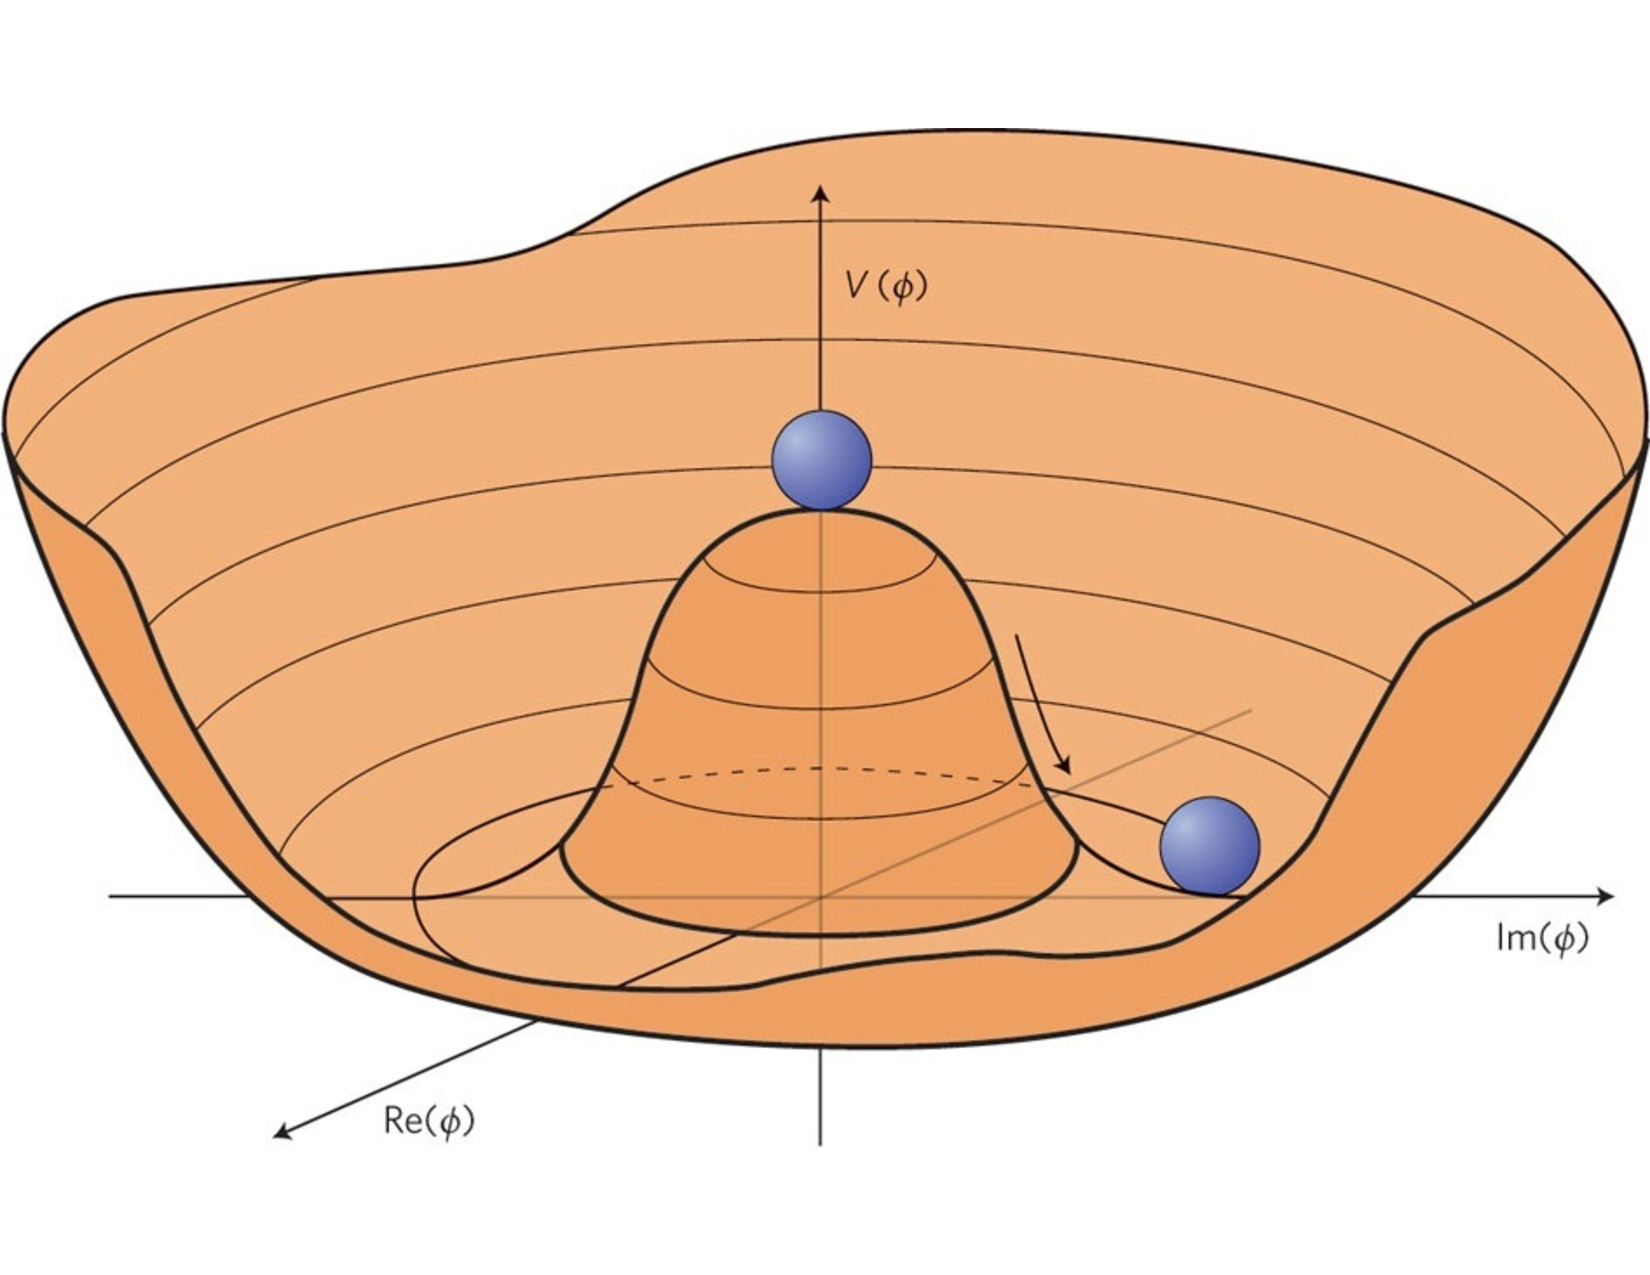
\includegraphics[width=0.55\textwidth]{phenomology_of_processes/plots/higgs_potential.pdf}
     \caption{
The potential $V\left(\phi\right)$ from Equation~\ref{eqn:v_pot} showing a non-stable state
at the origin and a stable state in the circular trough.
     }
     \label{fig:higgs_potential}
\end{figure*}



\section{Higgs Yukawa Couplings}
In addition to providing a mechanism for the $\PW$ and $\PZ$ bosons to gain mass in the SM, EWSB also
provides a mechanism for the fermions to acquire mass through their interactions with the Higgs boson
via Yukawa couplings. A Yukawa coupling is an interaction between a scalar field and a Dirac field
similar to,
\begin{equation}
V \approx h_{f}\bar{\psi_{f}}\phi\psi_{f},
\end{equation}

where the Dirac fields, $\psi$, describe fermions and the scalar field, $\phi$, is taken to be that of the Higgs boson. 
The introduction of a Yukawa interaction linking together the fermions and the Higgs boson,
results in massive fermions where their mass can be written as,
\begin{equation}
m_{f} = \frac{h_{f} v}{\sqrt{2}}
\label{eqn:yukawa_c}
\end{equation}

which covers the masses for the nine charged fermions: the three charged leptons and six quarks.
The EWSB mechanism nor the Yukawa interaction provide insight into the larger variety of fermion
masses. Instead, the fermion masses are taken as free parameters of the SM and the values
$h_{f}$ represent the Yukawa coupling parameter for each of the fermions.

The mass of nine charged fermions are known experimentally, most to very high precision.
The $\Pgt$ lepton is known to be $1776.82\pm0.16\MeV$~\cite{PDG}.
Knowing this, the $\Pgt$ lepton to Higgs boson Yukawa coupling can be calculated from theory
and compared against experimental results. 

Exploring the Higgs boson to fermions decay process is the most promissing way to directly probe
the Higgs boson Yukawa couplings. The Higgs boson decay process are discussed below in 
Section~\ref{sec:higgs_decays} where this discussion continues.

%with equation~\ref{eqn:yukawa_c},
%\begin{equation}
%h_{\Pgt} = \frac{\sqrt{2} \, m_{\Pgt}}{v} = \sqrt{2}\frac{1.78\GeV}{246\GeV} = 0.0102
%\label{eqn:yukawa_tau}
%\end{equation}



\section{Higgs Production}
The Higgs boson is produced through interactions with the particles it couples to in the SM
Lagrangian. Understanding the different production mechanisms for the Higgs boson
allows experimentalists to search for unique signatures in collisions to better
help separate Higgs bosons from the myriad other interactions occuring in collisions at the LHC.
At a hadron collider like the LHC, the Higgs boson production
mechanisms begin from initial states of quarks and gluons. The Higgs boson
only couples to massive particles eliminating direct gluon to Higgs boson processes
as is seen in Figure~\ref{fig:sm_forces} from the introduction.
However, the Higgs boson production process at the LHC which occures most often
begins with two gluons in the initial state, is called gluon fusion, and is discussed below.

Feynman diagrams of the leading Higgs boson production processes for
proton-proton based colliders, like the LHC, are shown in Figure~\ref{fig:higgs_feyn}. 
The cross sections for the leading Higgs boson production processes
are shown in Figure~\ref{fig:higgs_production}. The values for the leading
processes are approximately: gluon fusion ($ggH$) $\approx 49\pb$, 
vector boson fusion (VBF) $\approx 3.8\pb$, $\PW$ boson associated production ($\PW\PH$) $\approx 1.4\pb$,
and $\PZ$ boson associated production ($\PZ\PH$) $\approx 0.88\pb$~\cite{deFlorian:2016spz}. 
The top-quark associated process ($\ttbar\PH$),
which is found to be relatively insignificant in the following analyses, has a cross
section approximatly half the size of the next smallest one, $\PZ\PH$, where
$\ttbar\PH \approx 0.51\pb$ and accounts for less than 1\% of the total Higgs boson
cross section.


\begin{figure*}[htbp]
\centering
     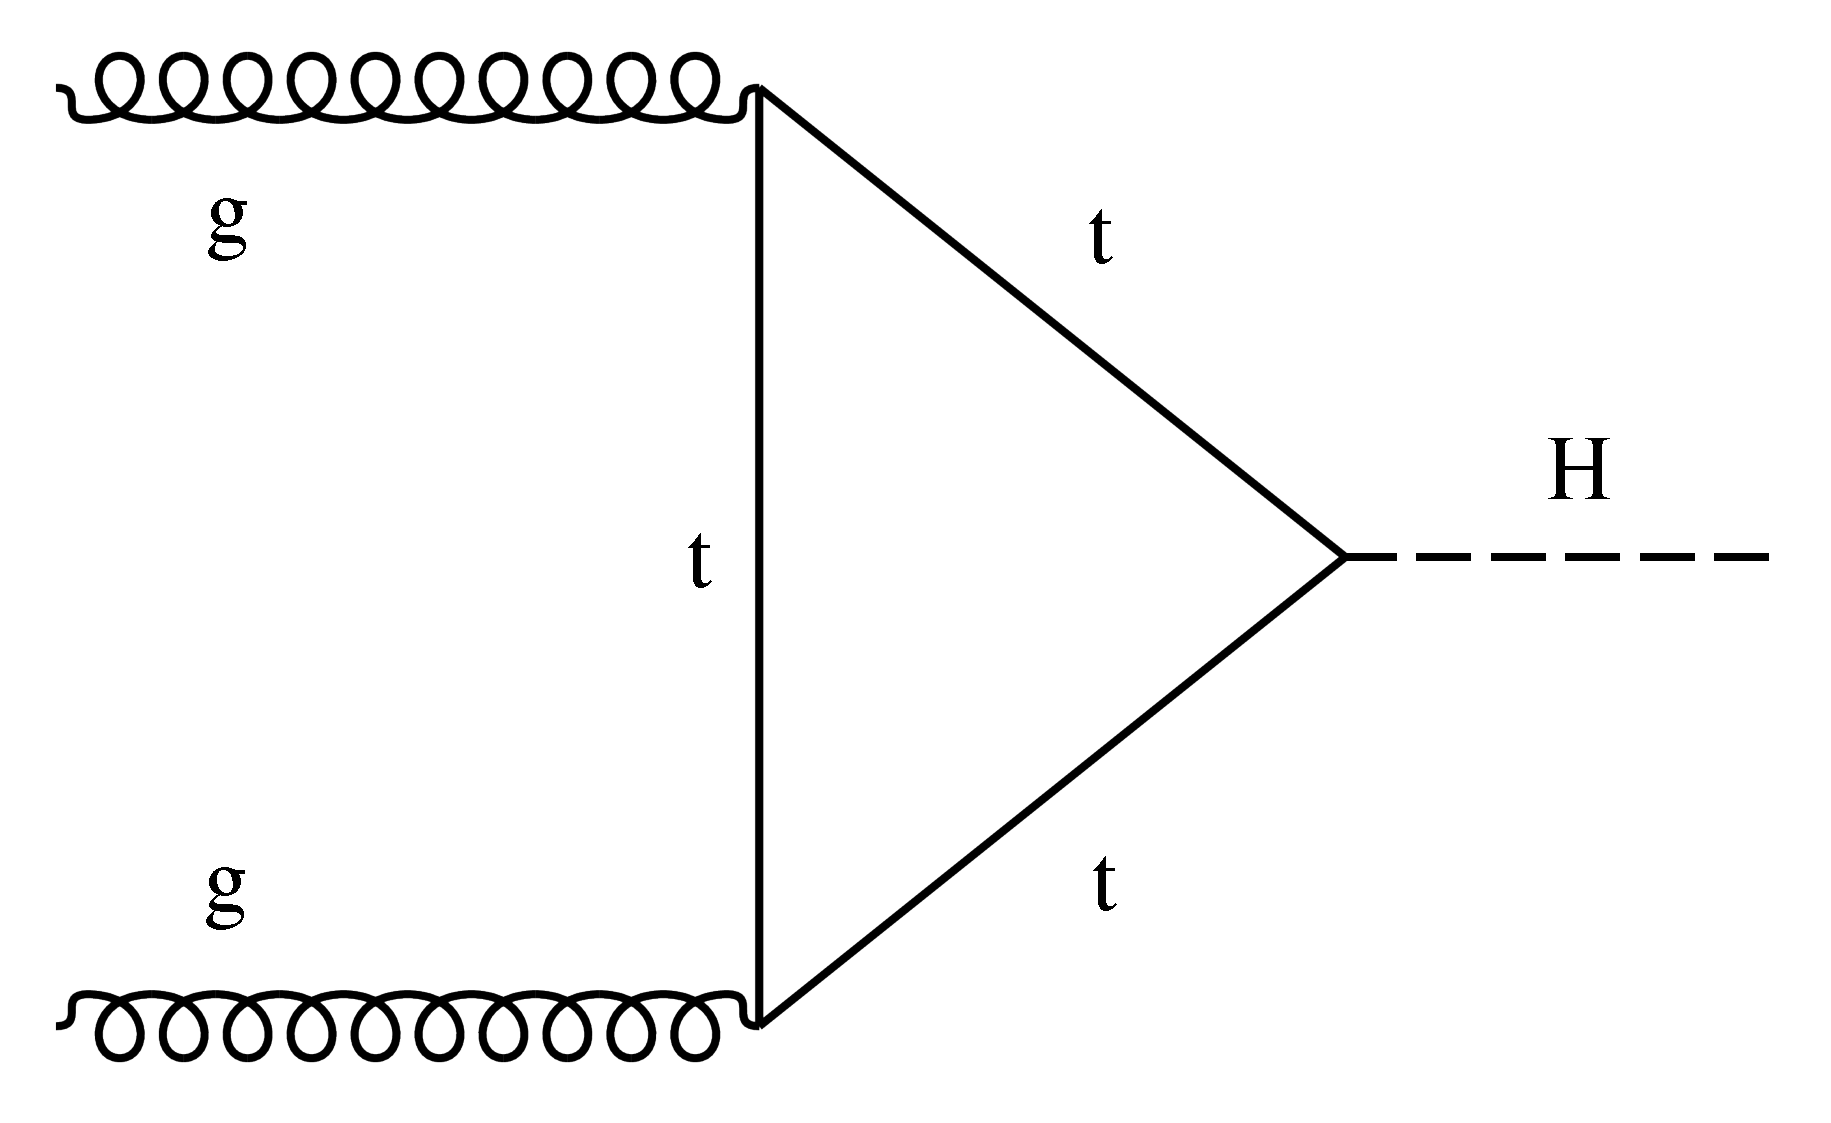
\includegraphics[width=0.35\textwidth]{phenomology_of_processes/plots/feyn_ggH.pdf}
     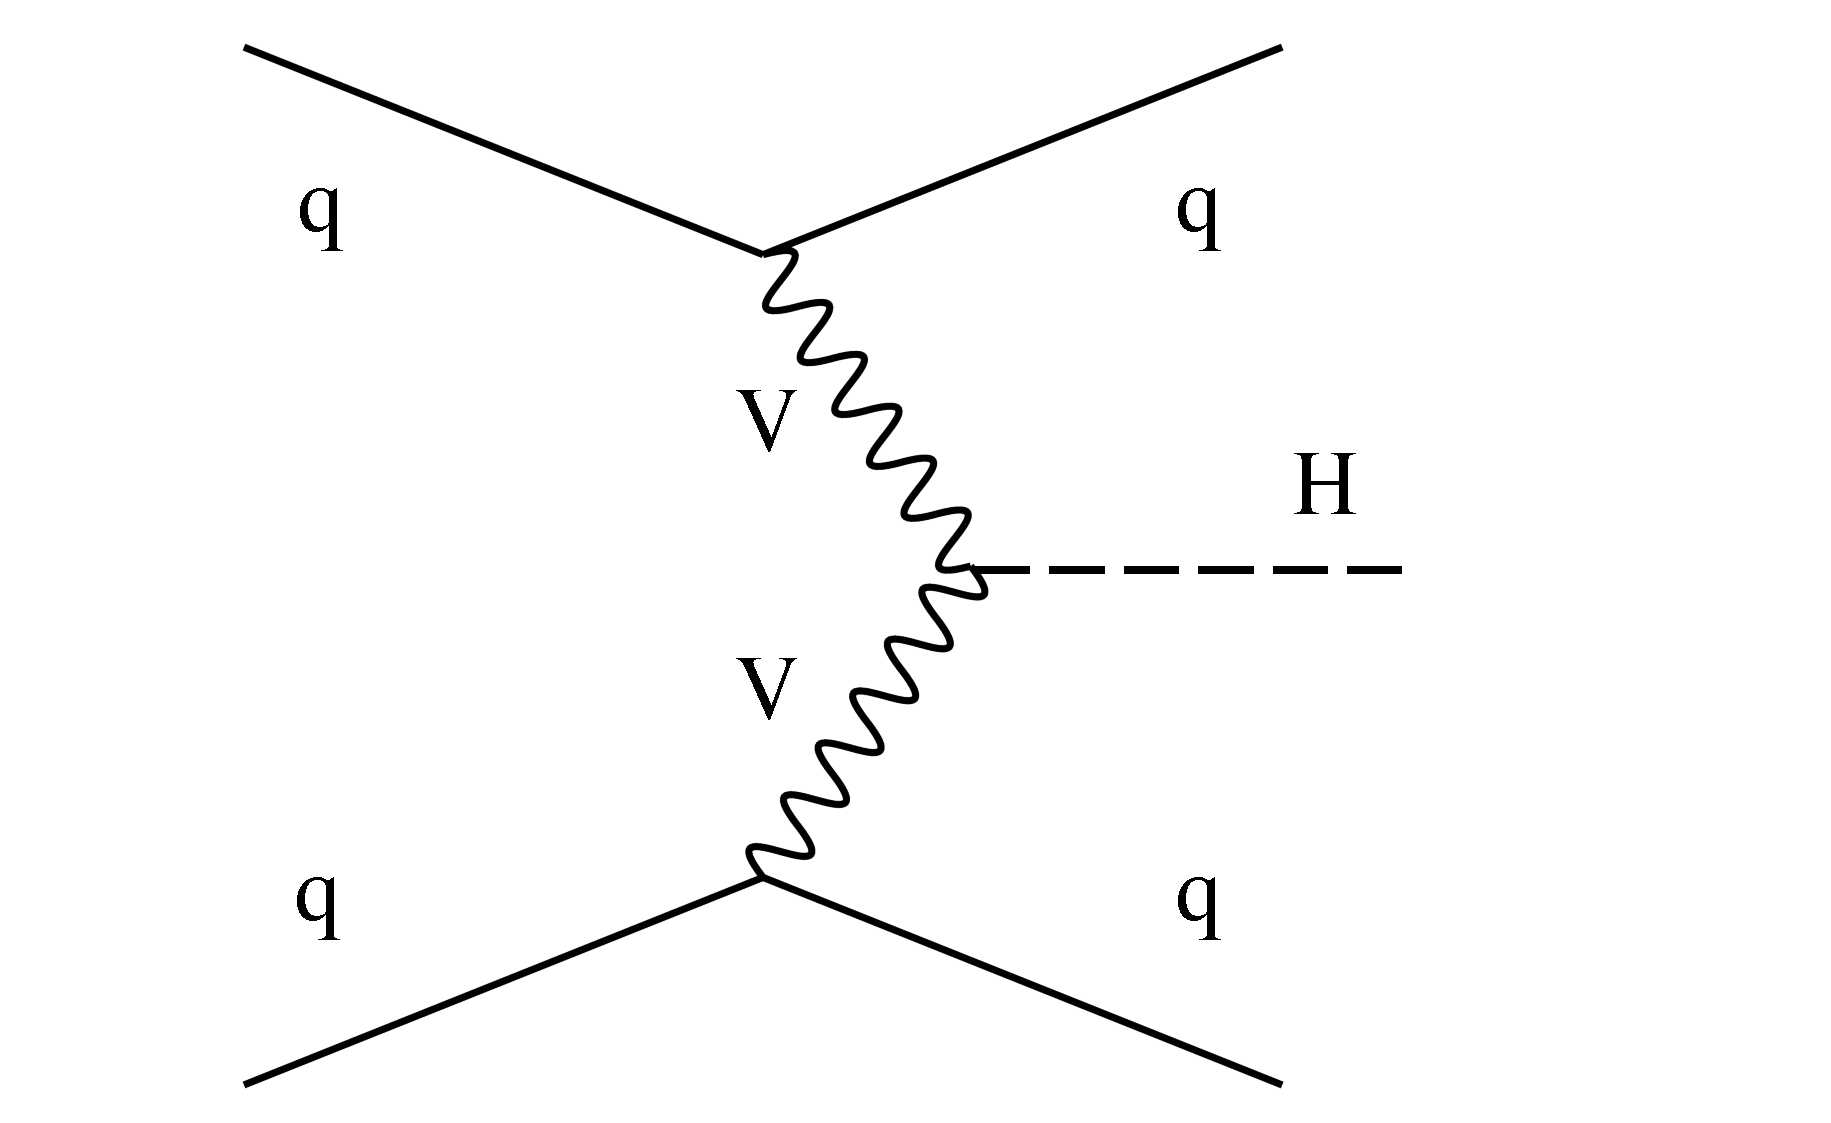
\includegraphics[width=0.35\textwidth]{phenomology_of_processes/plots/feyn_qqH.pdf}
     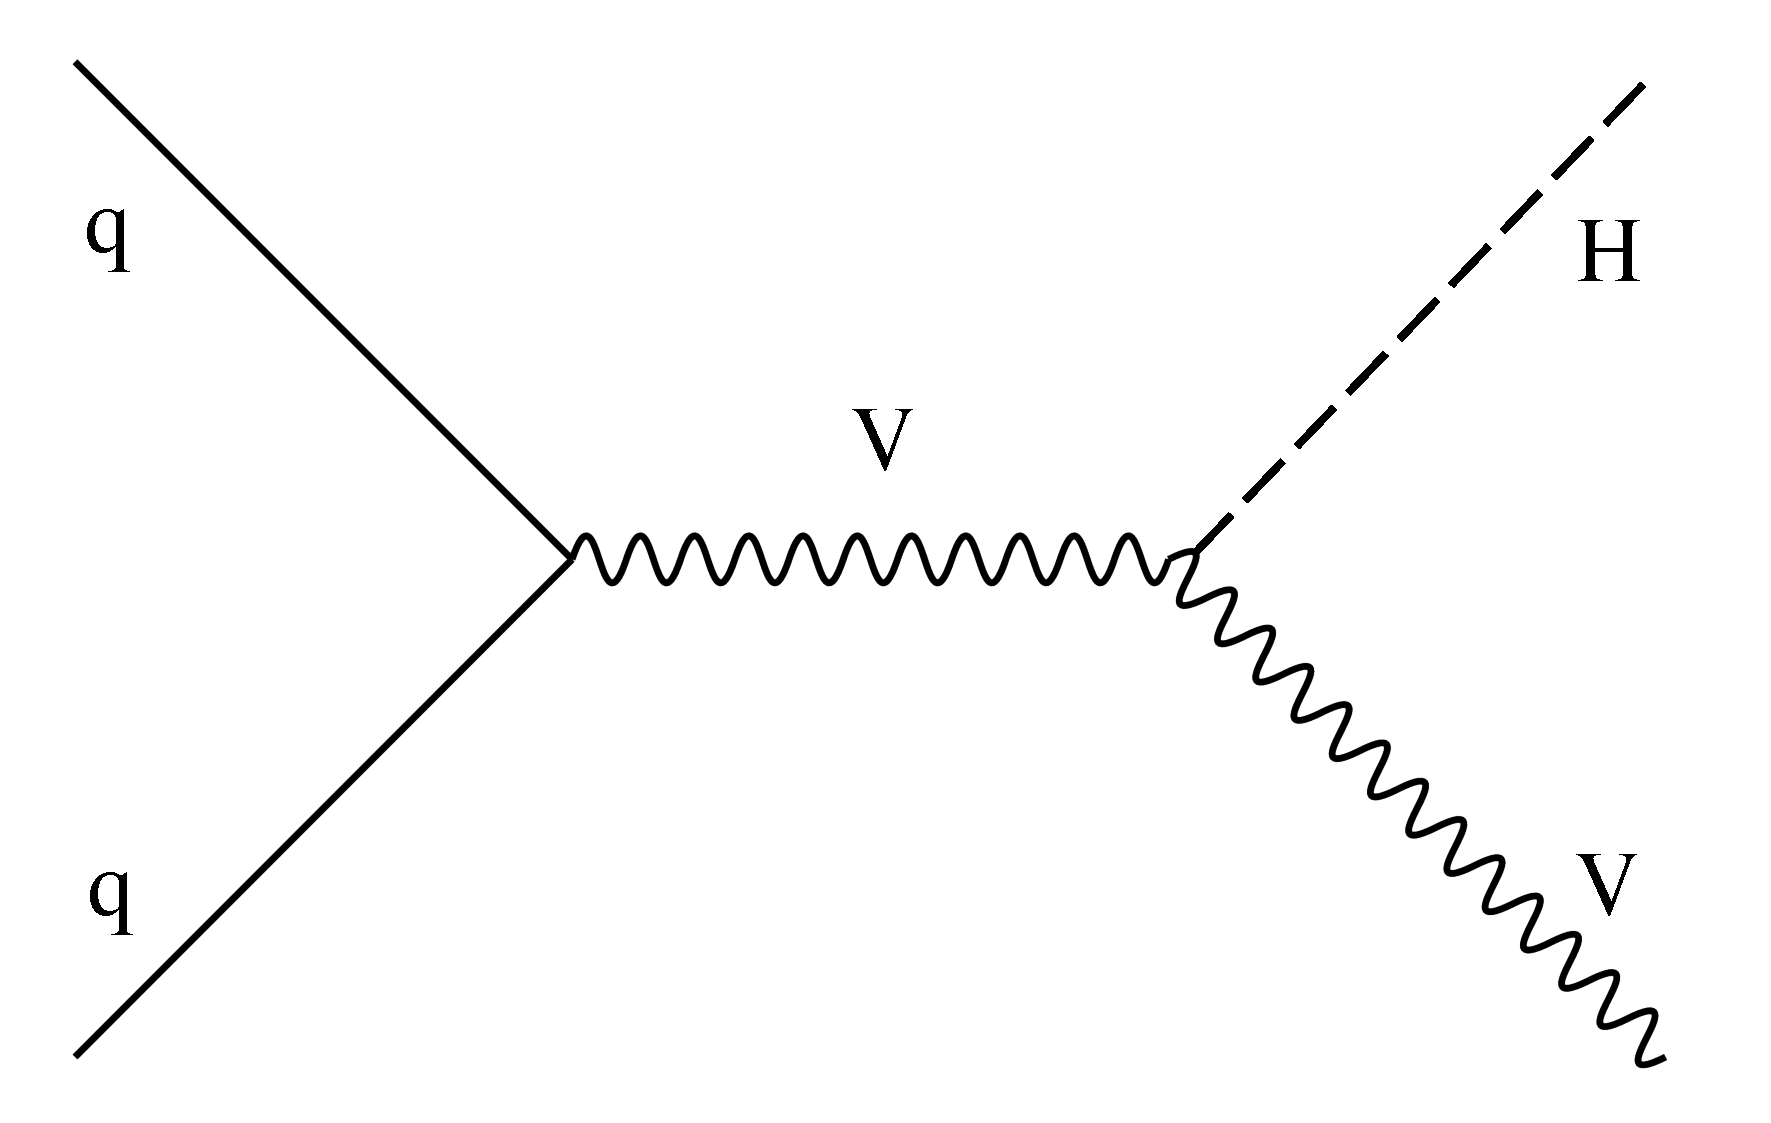
\includegraphics[width=0.35\textwidth]{phenomology_of_processes/plots/feyn_VH.pdf}
     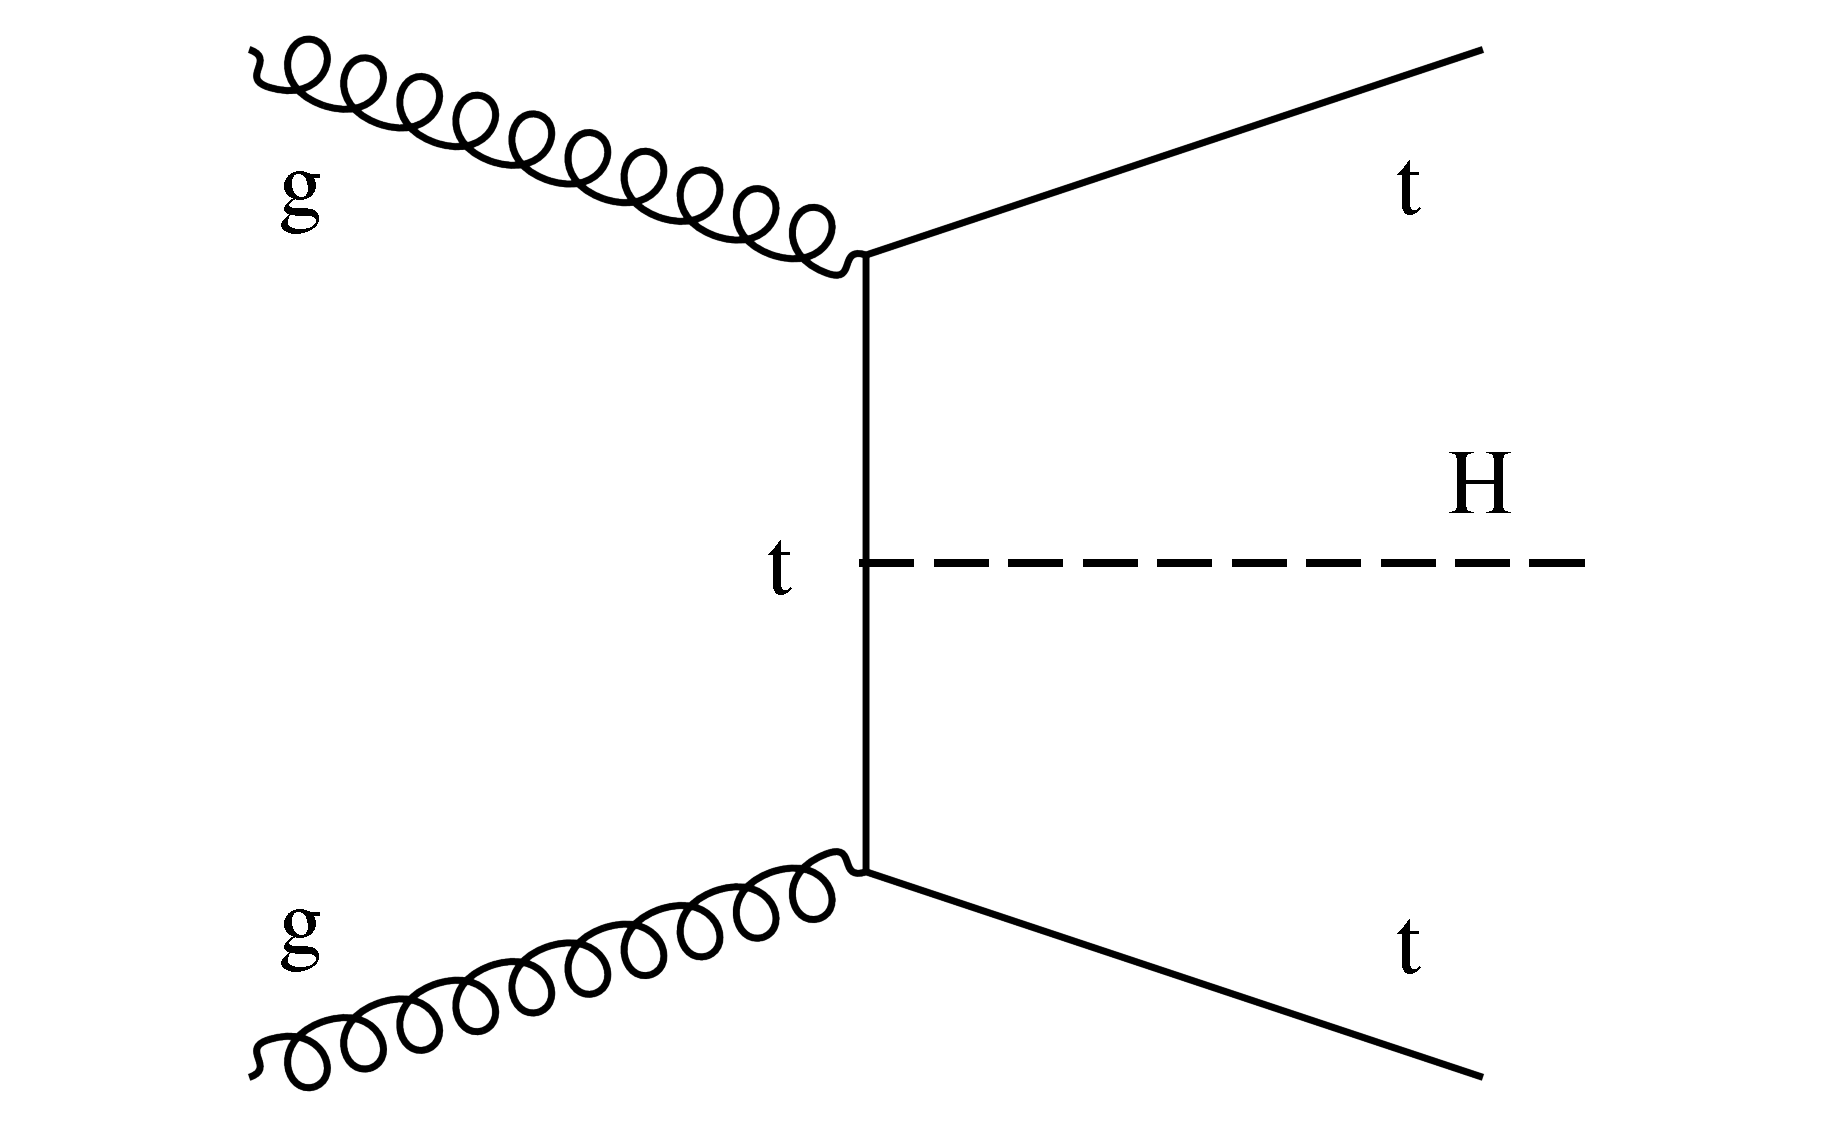
\includegraphics[width=0.35\textwidth]{phenomology_of_processes/plots/feyn_ttH.pdf}
     \caption{
Feynman diagrams representing the leading Higgs boson production processes.
Progressing in order of largest to smallest in production cross sections:
(top left) $ggH$, (top right) VBF, (bottom left)
$\PW\PH$ and $\PZ\PH$ processes,
and (bottom right) $\ttbar\PH$.
     }
     \label{fig:higgs_feyn}
\end{figure*}


\begin{figure*}[htbp]
\centering
     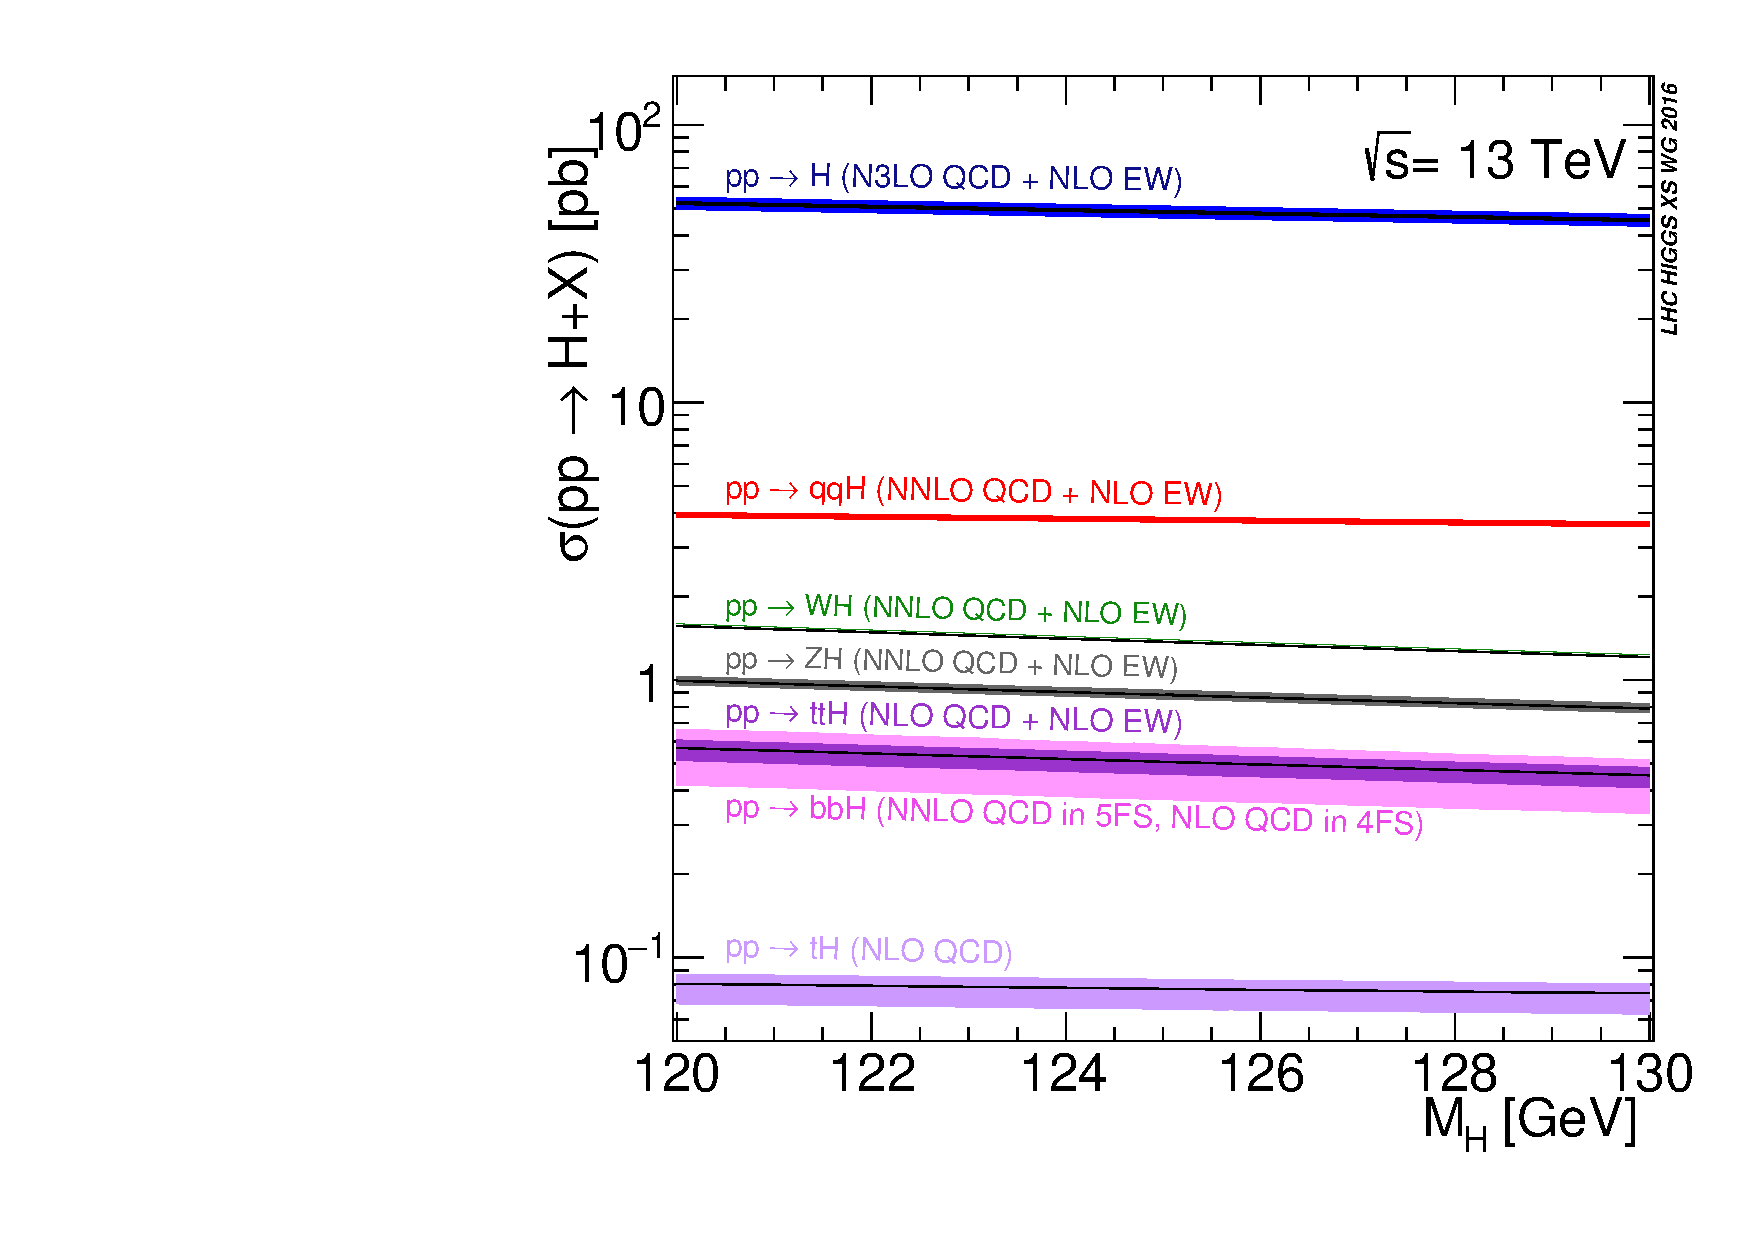
\includegraphics[width=0.65\textwidth]{phenomology_of_processes/plots/plot_13tev_H_sqrt.pdf}
     \caption{
The theorized Higgs boson production cross sections and their uncertainties
as a function of the Higgs boson mass, are shown. The $ggH$ process
is denoted as pp $\to$ H in the figure.
The CMS and ATLAS experiments have determined $\mH = 125.09\GeV$~\cite{Aad:2015zhl}.
     }
     \label{fig:higgs_production}
\end{figure*}


\subsection{Gluon Fusion}
The Higgs boson does not couple directly to gluons. Thus, the $ggH$ process is mediated by 
a virtual top quark loop, Figure~\ref{fig:higgs_feyn}. There are contributions from the other lighter quarks; however,
their contribution in the loop is suppressed proportional to $m^{2}_{q}$.
Because of the relatively large mass of the top-quark, to a very good approximation, 
the leading top-quark contribution can be evaluated in the limit 
$m_{t} \to \infty$~\cite{ELLIS1976292,Shifman:1979eb}.

Despite the $ggH$ process having the largest cross section, it is the hardest process to 
isolate from background events. A portion of $ggH$ produced Higgs bosons are produced in
in conjunction with one or multiple ``jets''~\ref{sec:obj_reco_jets}. In these
cases the Higgs boson recoils off of the jet creating a boosted topology
which is a more unique event signature. In this thesis the boosted event topology
is used as a handle in the ``Boosted'' event selection category discussed in
Section~\ref{sec:htt_categorization}. The majority of $ggH$ events are produced without
additional jets. While not having as clear or a handel to separat these events from
the background, these events are kept and are categorized into the less sensative ``0-Jet'' category.


\subsection{Vector Boson Fusion}
The second largest Higgs boson production process is VBF. This process originates by
the scattering of two quarks or anti-quarks. The scattering is mediated by the t-
or u-channel exchange of a $\PW$ or $\PZ$ boson. The Higgs boson is radiated off
of the $\PW$ or $\PZ$ boson~\cite{PhysRevD.70.113009}, Figure~\ref{fig:higgs_feyn}. 
The quarks or anti-quarks which are scattered
lead to the generation of high-energy jets present in the Higgs boson event.
This is a highly unique event signature and is used in nearly all Higgs analyses
to identify Higgs bosons produced via VBF. In this thesis, events with two high-energy
jets consistent with VBF topology are categorized into a ``VBF'' category for analysis.


\subsection{Associated Production}
The Higgs boson associated production mechanism makes up the third and fourth largest
Higgs boson cross sections for $\PW\PH$ and $\PZ\PH$ respctively. Both processes are 
depicted in the lower left Feynman diagram in Figure~\ref{fig:higgs_feyn} where
the $V$ represents vector bosons covering both $\PW$ and $\PZ$. Associated
production is often called Higgs-strahlung in reference to bremsstrahlung, the
process where a deccelerating charged particle emits radiation, often an electron
emitting a photon. In the case of Higgs-strahlung, the vector boson created 
from two initial state quarks or anti-quarks emits a Higgs boson. The associated
production event topology is quite unique with the presence of a $\PW$ or $\PZ$
boson plus a Higgs boson. In this thesis there is an analysis targeted at each
of these process, $\PW\PH$ and $\PZ\PH$.



\section{Higgs Decays}
\label{sec:higgs_decays}
After a Higgs boson is produced, it will decay extremly rapidly. The theorized lifetime of a Higgs
boson particle is $1.6 \times 10^{-22}$ s~\cite{Dittmaier:2012vm}. This means that when created
inside of the CMS detector, a Higgs boson will always decay
within the CMS detector. In all Higgs boson analyses, experimentalists search for the
signatures of the decay products in energy deposits in their detectors, not the Higgs
boson itself. There are multiple possible decay
paths each with its own branching ratio; the largest branching ratio
processes are shown in Figure~\ref{fig:higgs_decay}. The $\htt$ process has a branching
ratio of approximately 6.3\% with a relative theoretical uncertainty of 
$\pm5.7\%$~\cite{deFlorian:2016spz} for $\mH = 125\GeV$. This places $\htt$ below $\PH\to\bbbar$, 
$\PH\to\PW\PW$, and $\PH\to\Pg\Pg$ in branching fraction.

\begin{figure*}[htbp]
\centering
     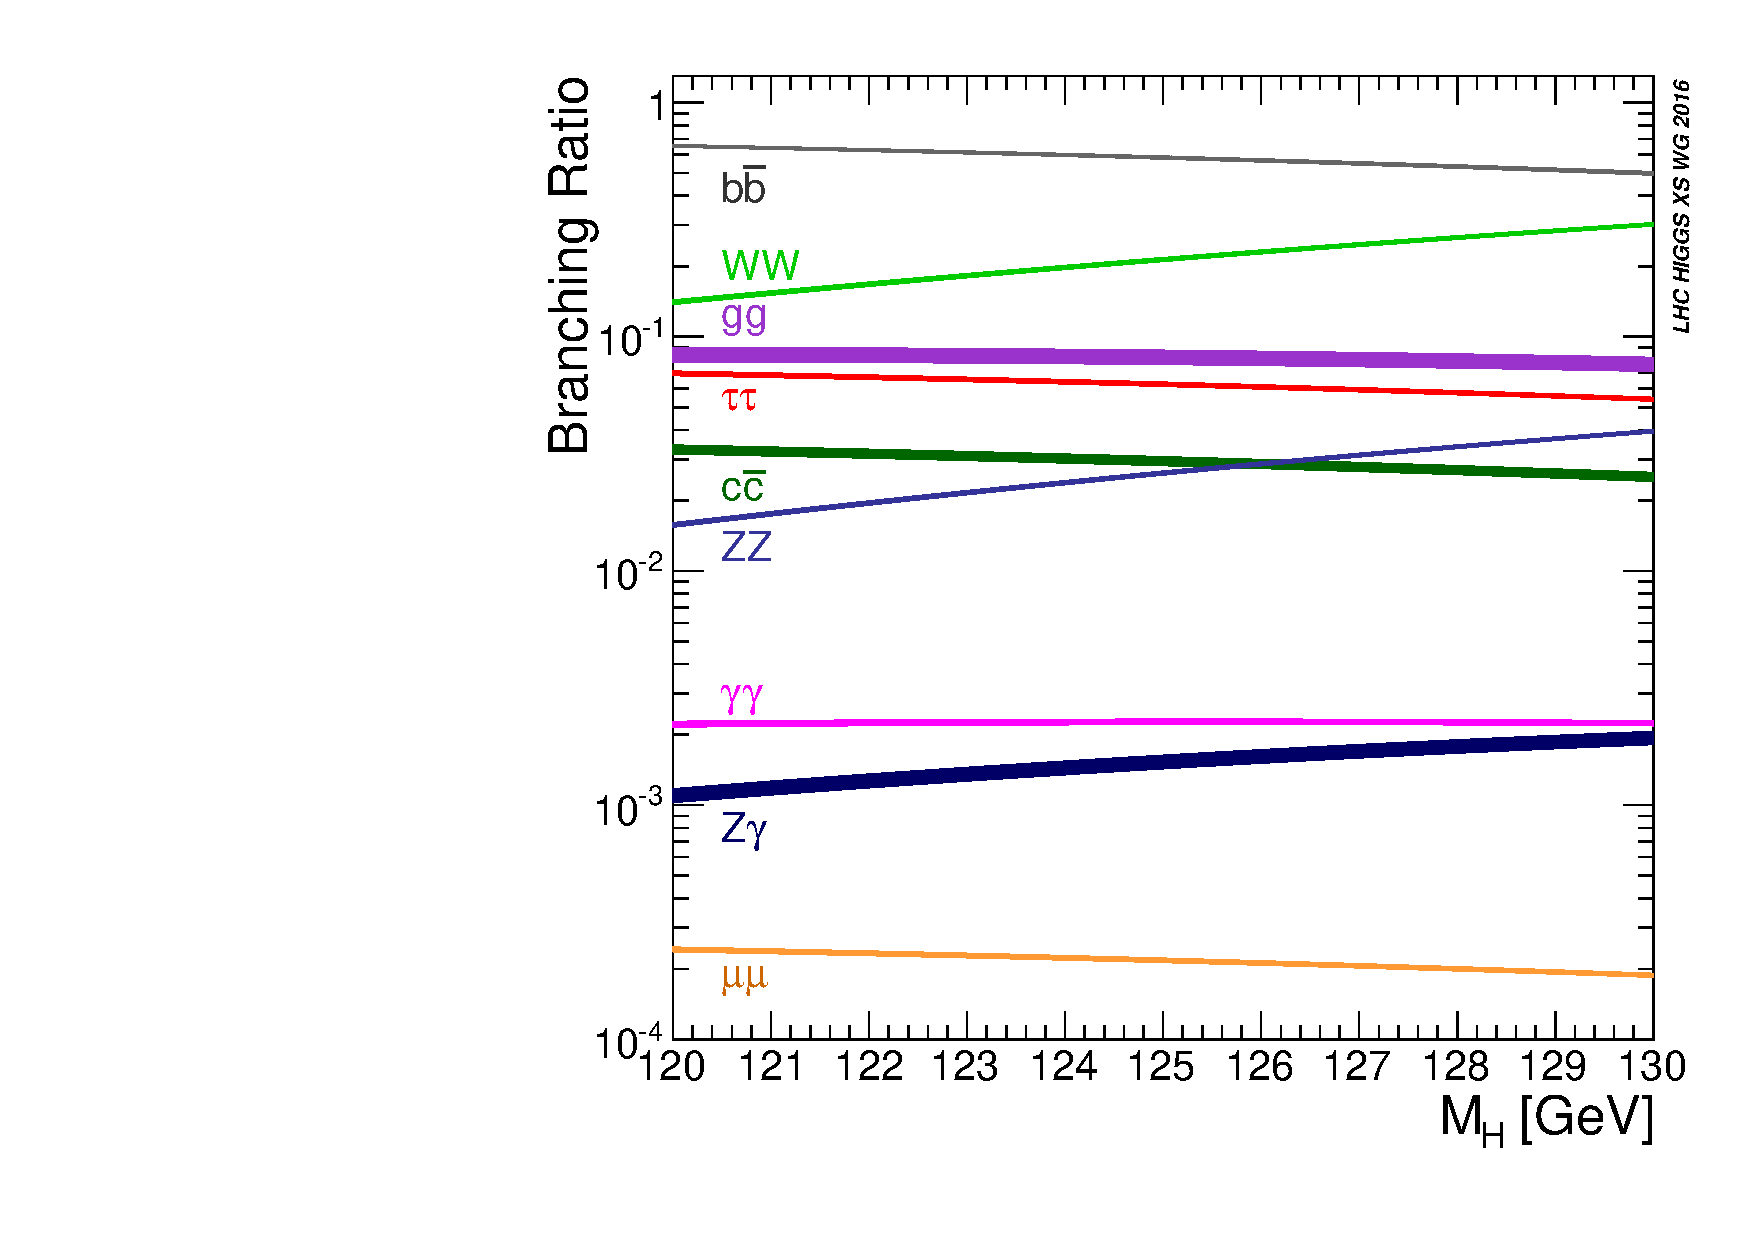
\includegraphics[width=0.65\textwidth]{phenomology_of_processes/plots/SMHiggsBR_YR4-square.pdf}
     \caption{
The different theorized Higgs boson decay process are shown as a 
as a function of the Higgs boson mass.
The CMS and ATLAS experiments have determined $\mH = 125.09\GeV$~\cite{Aad:2015zhl}.
     }
     \label{fig:higgs_decay}
\end{figure*}

The leading Higgs boson decay processes each have certain advantages and disadvantages
to elucidating the properties of the Higgs boson. The dominant Higgs boson decay 
process, $\PH\to\bbbar$, comprises well over half of all Higgs boson decays yet suffers
from very large background processes making it difficult to distinguish Higgs bosons.
Additionally, the $m_{\bar{b}b}$ resolution is limited making the expected Higgs boson
signal a broad distribution ontop of a large background~\cite{PDG}.
The $\PH\to\PW\PW$ process has a large branching ratio which is reduced after requiring
$\PW\to\ell + \bar{\nu}$ where $\ell$ is a charged lepton. Additionally, the presence of neutrinos
in the final state decreases the Higgs boson mass resolution, $\approx 20\% \, \mH$~\cite{PDG}.
The $\PH\to\Pg\Pg$ is an extraordinairly difficult process to attempt to observe at a
hadron collider because the final state provides no helpful handles to disintangle it from
the dominant multijet backgrounds.

The $\htt$ process is the largest direct Higgs boson to leptons decay process.
This provides a unique opportunity to probe the Higgs boson Yukawa couplings to the leptons,
while both the $\PH\to\bbbar$ and $\htt$ processes can directly probe the Higgs boson
Yukawa couplings to fermions. Similar to the $\PH\to\PW\PW$ process, $\htt$ has neutrinos
in the final state making reconstructing the Higgs boson mass non-trivial.
The relative size of the backgrounds with event signatures similar to the Higgs boson
are much smaller for the $\htt$ process versus the $\PH\to\bbbar$ process. This is one
of the significant benefits of studying the Higgs boson through the $\htt$ process.

In this thesis, the various Higgs boson production cross sections and branching fractions 
for Higgs boson production, and their corresponding uncertainties are taken from 
References~\cite{deFlorian:2016spz,Denner:2011mq,Ball:2011mu} and references therein.





%\chapter{The CMS Experiment and the CERN LHC}

\section{The LHC}

\subsection{LHC Pre-Acceleration}

\subsection{LHC Acceleration}

\section{The CMS Experiment}

The Compact Muon Solenoid (CMS) detector is located at point 5 along the LHC ring near Cessy, France. It is
one of the two large general purpose physics detectors in operation at the LHC along with ATLAS. The
CMS detector was inspired by decades of previous high energy particle physics detectors and has as its
primary purpose to detect and measure the characteristics of the Standard Model Higgs boson. The 
detector was designed and built targeting high efficiency and energy resolution for specific Higgs 
boson decay modes. The high granularity of the electromagnetic calorimeter and excellent energy
resolution make it perfect for reconstructing photons from $\PH \to \gamma\gamma$ decays. The
strong, 3.8T magnetic field combined with the muon spectrometer provide excellent Higgs boson
mass resolution in the $\PH \to \PZ\PZ \to \Pgm\Pgm\Pgm\Pgm$ decays. The detector is a large
cylinder 15.0m in diameter and 28.7m in length. It has a mass of approximately 14,000,000kg.

The CMS detector is built out of many subdetectors. Progressing radially outwards from the collision point,
there is firts the silicon pixel tracker the the silicon strip trigger sytems. Next is the 
electromagnetic calorimeter followed by the hadronic calorimeter. These systems are all contained
within the bore of the CMS superconducting magnet. After the the solenoid there are additional subsystems
embedded within the steel flux-return yoke. In the central region of the detector, there is an 
outer portion of the hadronic calorimeter, and lastly, the muon spectrometer. These systems can all be viewd in
Figure~\ref{fig:cms_detector}.

\begin{figure*}[htbp]
\centering
     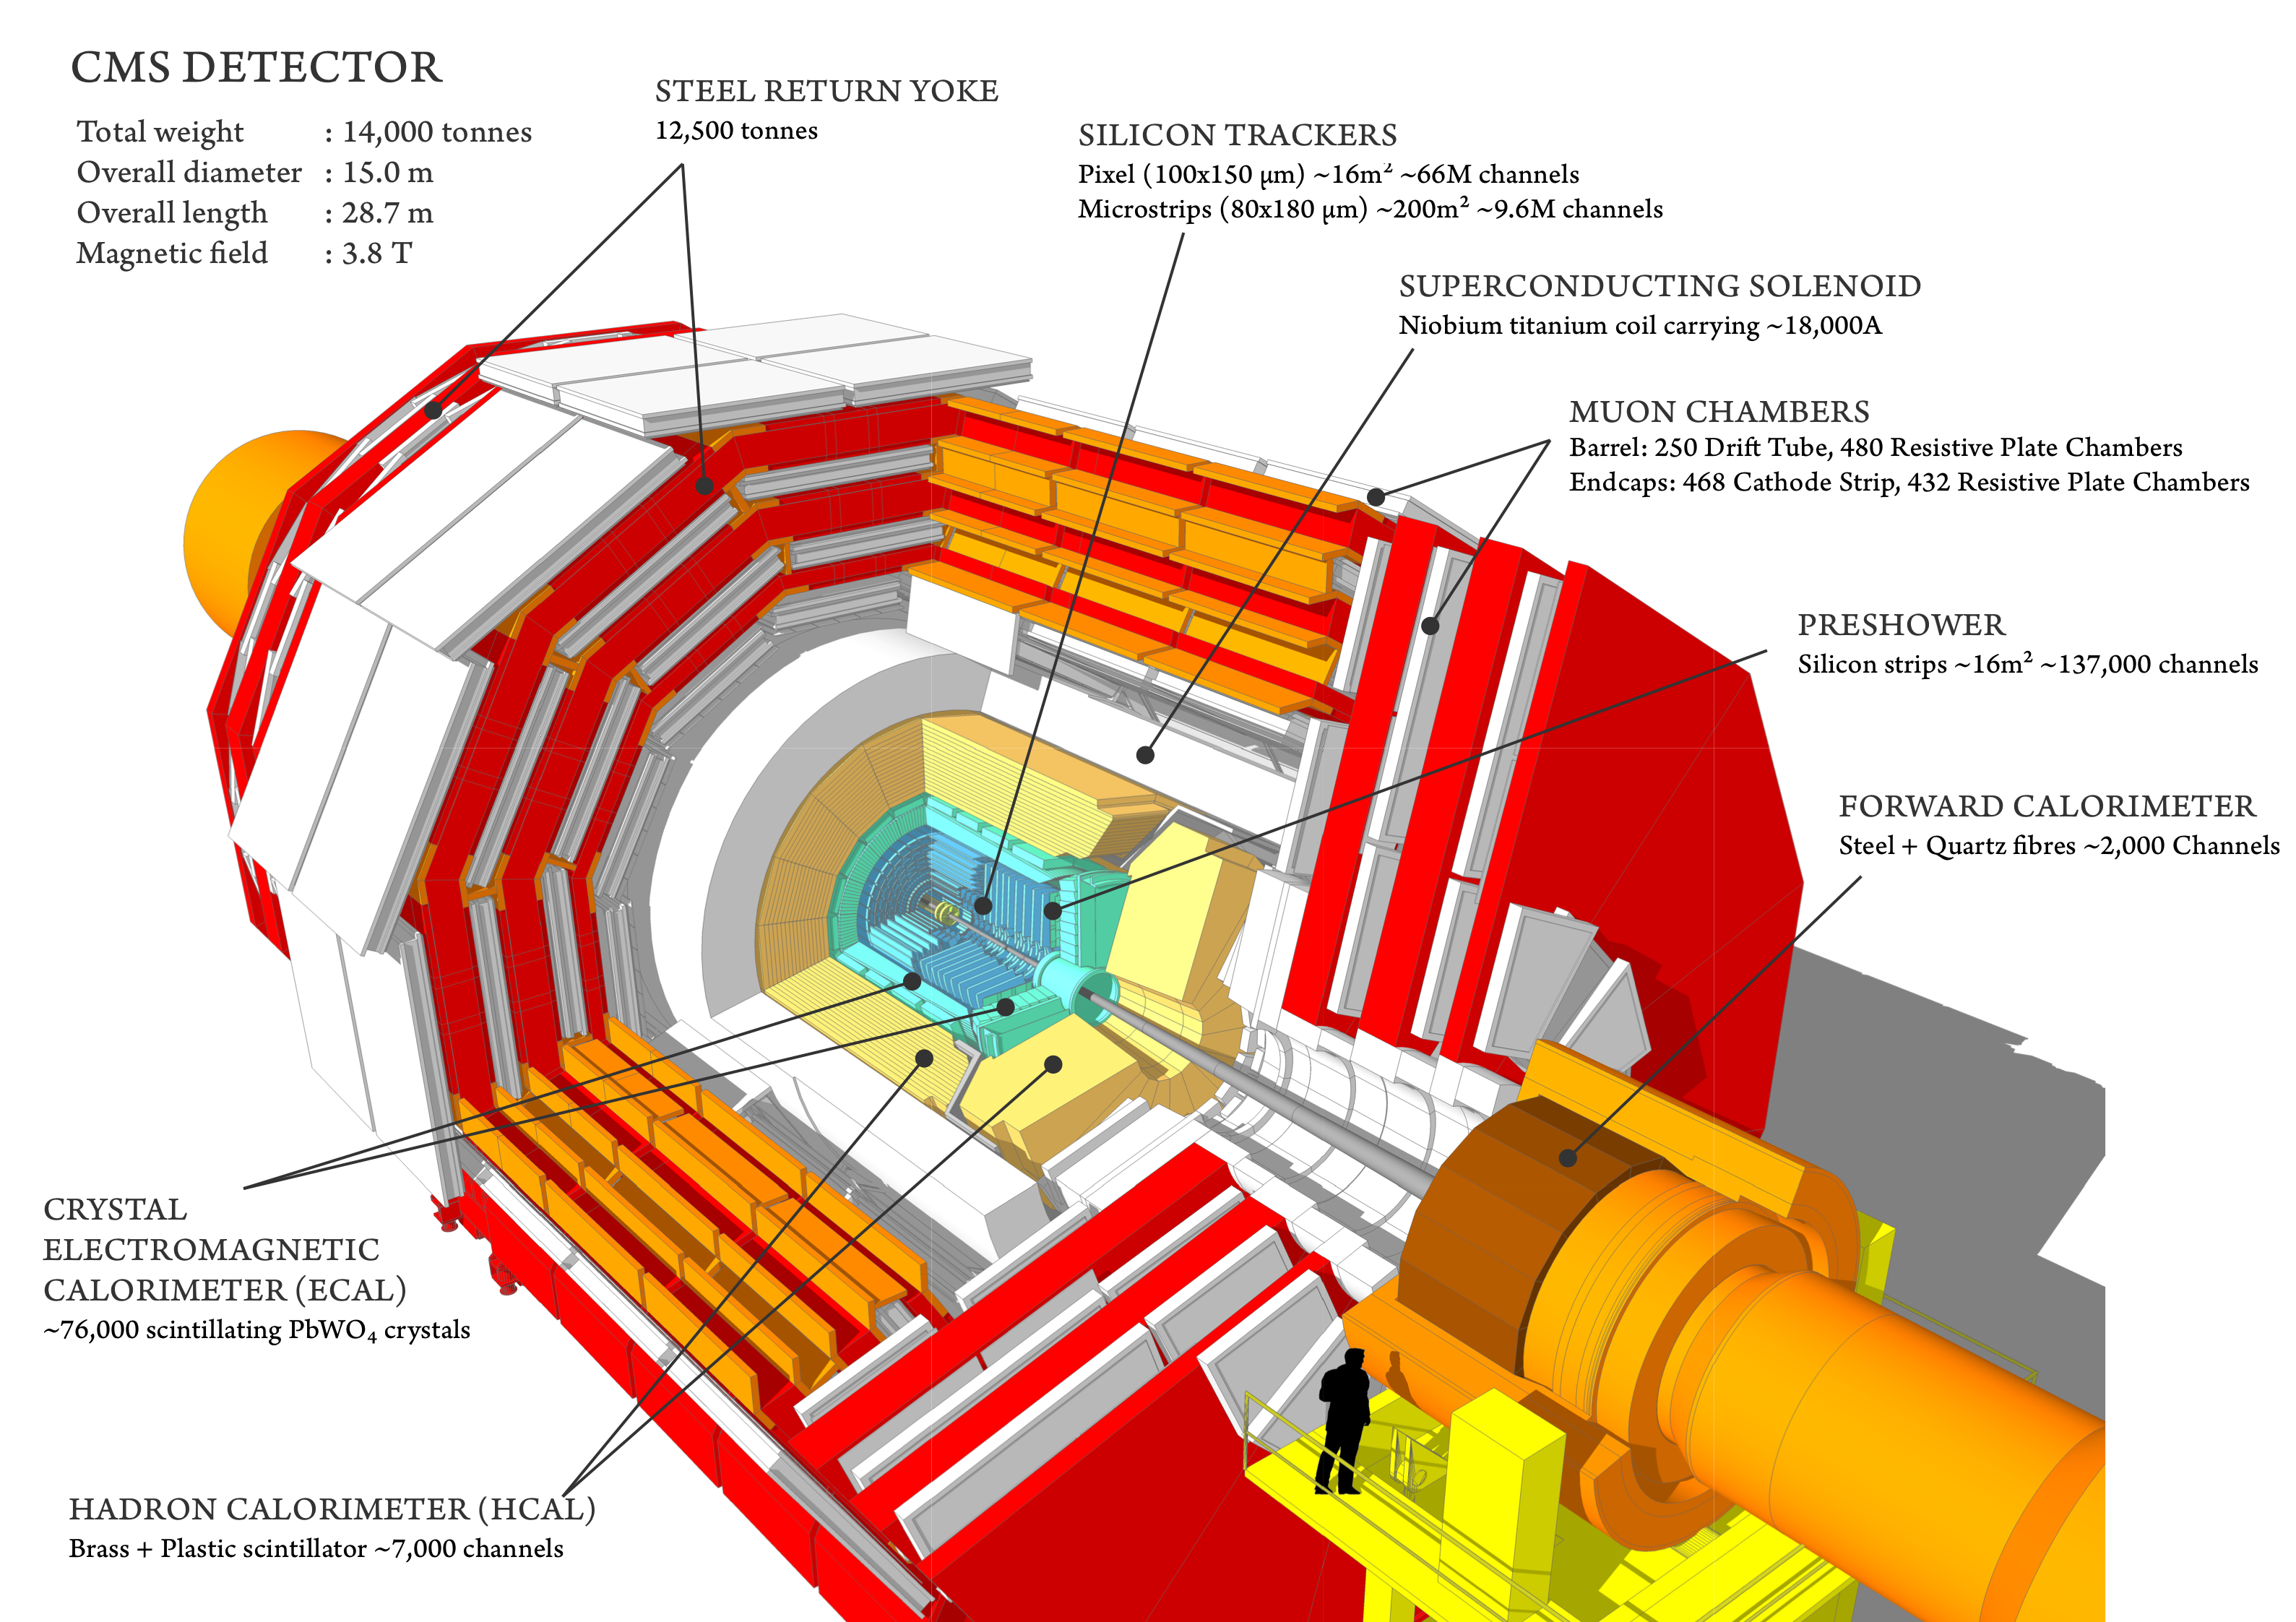
\includegraphics[width=1.0\textwidth]{cms_and_lhc/plots/cms_detector.png}
     \caption{
     }
     \label{fig:cms_detector}
\end{figure*}

Information from the 40 MHz proton-proton collisions is aggregated by a central data acquisition system
and filtered before storage by a two-tiered trigger system~\cite{Khachatryan:2016bia}. 
The first level of the trigger sytem is composed of custom hardware processors, uses information 
from the calorimeters and muon detectors to select events at a rate of around 100 kHz. The second level of
the trigger, known as the high-level trigger, consists of a farm of commercial processors further
filtering out non-interesting data events resulting in a final event rate of about 1 kHz which is stored
for futher processing an analysis.



\subsection{Geometry}
To understand the CMS detector, an understanding of the geometry and coordinate system used by the 
CMS detector is necessary. The CMS detector is a hermetic, cylindrical particle detector surrounding
a central region designed to be the location of the $\pp$ collisions delivered LHC. This middle
point, inside the LHC beam pipe is designated as the origin for the CMS coordinate system, (0,0,0) in
$(x, y, z)$ coordinates. Positive $x$ points towards the center of the LHC ring.
Positive $y$ points vertically upwards. The positive $z$ direction is along the LHC ring in the
clockwise direction when viewed from above. These $(x, y, z)$ coordinates are commonly transformed
into quasicylindrical coordinates when referring to particles, $(\pt, \eta, \phi)$. For a particle,
$\pt$ is:

\begin{equation}
\pt \equiv \sqrt{p^{2}_{x} + p^{2}_{y}}
\end{equation}

$\eta$ is defined using $\theta$ from traditionally spherical coordinates.

\begin{equation}
\eta \equiv -ln\bigg[\tan\bigg(\frac{\theta}{2}\bigg)\bigg]
\end{equation}

$\phi$ is defined in the $x-y$ plane.



\subsection{Superconducting Magnet}
The CMS superconducting magnet, as is noted in the collaboration name, is one of the most fundamental
pieces of the CMS experiment. The superconducting magnet bends the trajectories of charged particles
within the CMS detector. The curve in the flight path of a charged particle can be used to help
calculate the energy or momentum of the particle in accordance with the Lorenetz force.
Within the CMS detector, where the electric field is negligible compared to the magnetic field
from the superconducting magnet, the Lorentz force can be written as~\ref{eqn:lorentz}

\begin{equation}
\textbf{F} = q\textbf{v} \times \textbf{B}
\label{eqn:lorentz}
\end{equation}

relating the mass, acceleration and momentum of a particle with the magnetic field.

The CMS superconducting magnetic is constructed from a 4-layer winding of stabalised
reinfored NbTi conductor. When in operation, the magnet is kept in a superconducting state
by cooling it with liquid helium to a temperature of 4.6 Kelvin. With a nominal current
of 19.14 kA the superconducting solenoid magnet is able to produce a roughly uniform
magnetic field of 3.8 T within its central bore. The magnetic field created is roughly
100,000 times stronger than the Earth's magnetic field. Stronger the magnetic fields produce
more higly curved particle trajectories leading to better momentume and energy measurements.
The central bore is only 6.3 m in diameter
leaving limited room for the CMS tracker and calorimeter systems.



\subsection{Inner Tracking System}
The inner tracking system is composted of two subdetectors, the pixel tracker and the
strips tracker. They are designed to deliver precise and efficient measurement of
the trajectories of charged particles propagating outwards from the LHC delivered
$\pp$ collisions. The tracking systems can be used to reconstruct the origins of
the tracks to reconstruct collision points and secondary decay vertices. The
tracking systems surround the interaction point and have a length of 5.8m and 
diameter of 2.5m. Both the pixel and strip trackers have cylindrical barrel
layers and disk-like endcap layers. A schematic of the track systems
can be seen in Figure~\ref{fig:cms_tracker}.

The pixel tracker has three barrel layers at radii between 4.4cm and 10.2cm. The
close proximity to the interaction point is helpful for track seeding and vertex
reconstruction discussed in the track reconstruction section~\ref{sec:pf_tracks}.
The silicon strip tracker is composed of 10 barrel detection layers extending 
outwards to a radius of 1.1m. During the 2016-2017 extended year end techincal stop,
the pixel tracker was upgraded to have a fourth detection layer. As 2017 data is not used
in the analyses presented here, details of this upgrade are omitted.
The endcaps of the pixel tracker consist of 2 disks which extend the $\eta$ 
range of the detector to $\abs\eta < 2.5$. The same $\eta$ range is covered in the
strips tracker with 12 disks on each side of the barrel.

\begin{figure*}[htbp]
\centering
     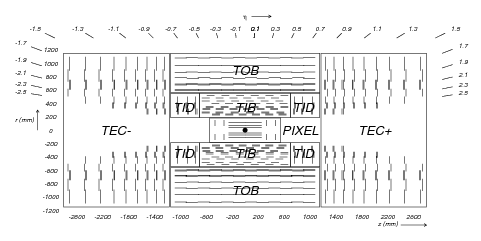
\includegraphics[width=0.8\textwidth]{cms_and_lhc/plots/cms_tracker.png}
     \caption{
Schematic cross section through the CMS tracker. Each line represents a detector module. 
Double lines indicate back-to-back modules which deliver stereo hits.
     }
     \label{fig:cms_tracker}
\end{figure*}

The pixel tracker contains about 66 million individual pixels. The strips tracker
contains 9.3 million individual strips. This phenominal resolution is necessary
because of the extremely high particle flux through the tracker. During 2016 data
taking, it is estimated that there were $\mathcal{O}( 1000 )$ particles 
traversing the tracker from the more than 20 overlapping simultaneous proton-proton 
interactions during a single bunch crossing. The tracker measures the $\pt$ of 
charged hadrons in the barrel region with a resolution of 1\% for $\pt < 20\GeV$.
The information from the tracker systems is
not used by the L1 trigger. However, the tracker information is heavily used by the HLT to
reduce the event rate from the L1 trigger, 100kHz, to the final rate of 100Hz.

A serious concern during the design of the tracker systems was the amount of
material necessary to build the systems. All of the electronics, hardware, 
cooling systems and wiring contribute to the tracker material budget. Any and all material
located between the interaction region and the calorimeters will reduce the precision 
of the calorimeter energy measurements as well as potentially degrade the track-based
measurement of the energy of a particle. This is because of potential electromagnetic
and/or nuclear interactions between the particle and the tracker material. Figure~\ref{fig:cms_tracker_thickness}
shows the material budget in terms of interaction lengths and radiation lengths as a function
of $\eta$ for the tracker systems.

\begin{figure*}[htbp]
\centering
     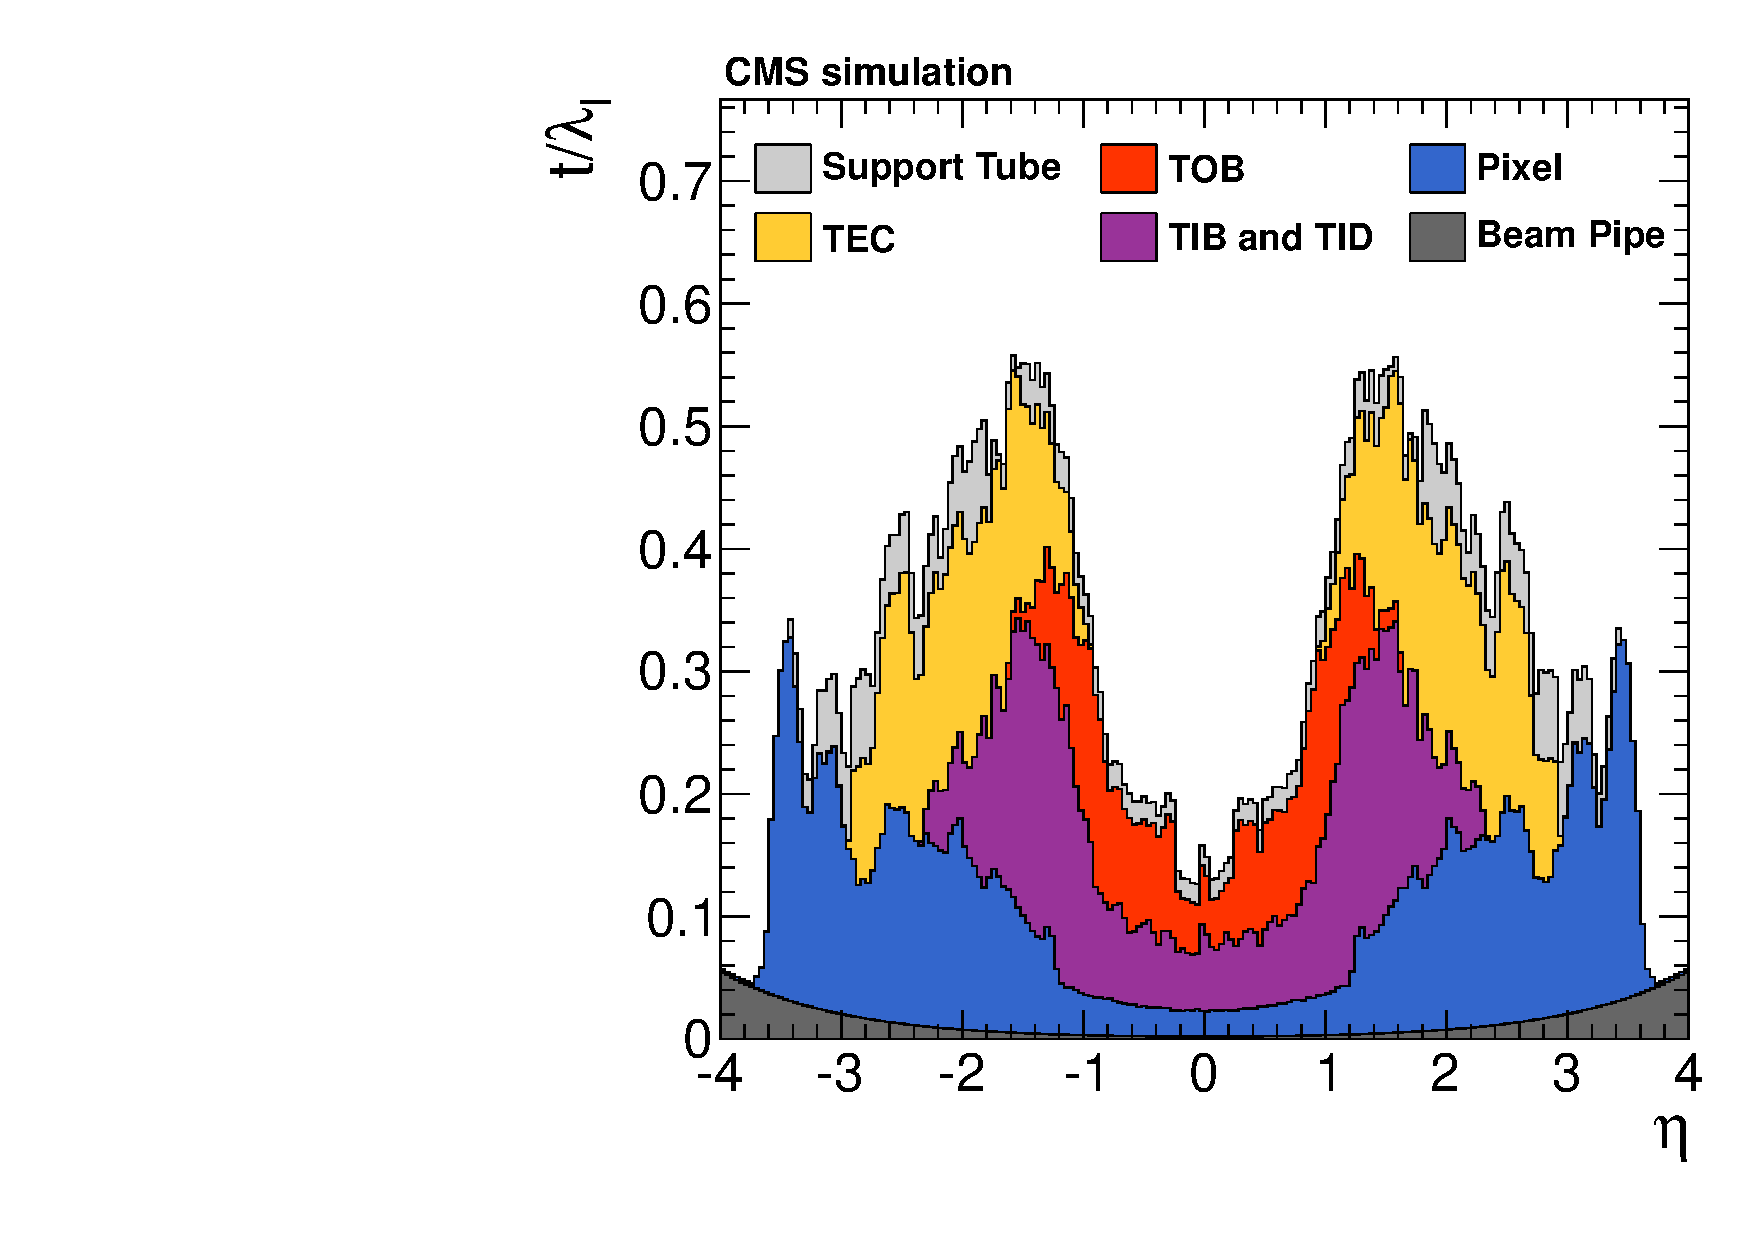
\includegraphics[width=0.4\textwidth]{cms_and_lhc/plots/cms_tracker_thickness_radiationL.pdf}
     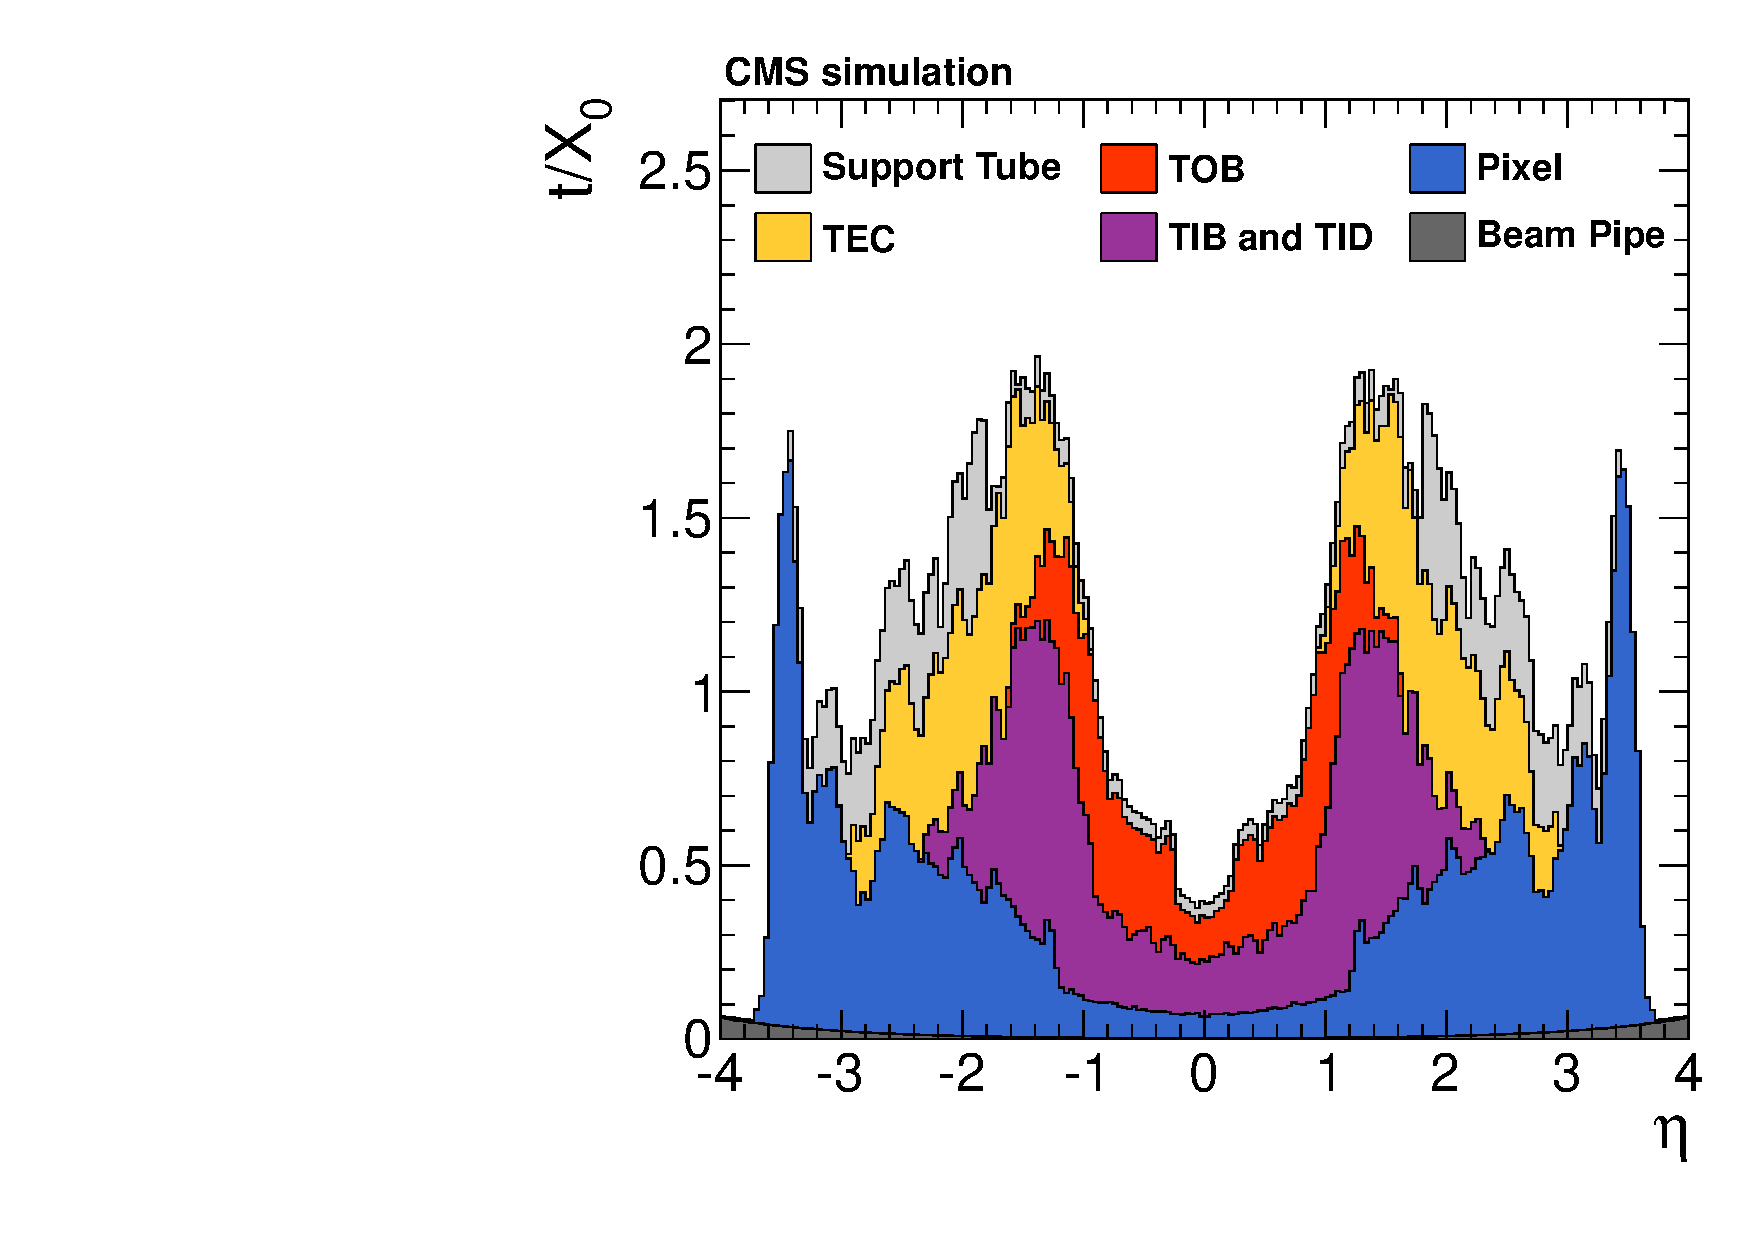
\includegraphics[width=0.4\textwidth]{cms_and_lhc/plots/cms_tracker_thickness_interactionL.pdf}
     \caption{
Total thickness $t$ of the inner tracker material expressed in units of interaction lengths 
$\lambda_{l}$ (left) and radiation lengths $X_{0}$ (right), as a function of the pseudorapidity $\eta$.
     }
     \label{fig:cms_tracker_thickness}
\end{figure*}



\subsection{Electromagnetic Calorimeter}
The electromagnetic calorimeter (ECAL) is a homogeneous calorimeter made of lead 
tungstate $(\textrm{PbWO}_{4})$ crystals. There are 61200 individual crystals mounted
in the barrel region with 360 crystals completing a ring in $\phi$ and 170 crystals
spanning the barrel $\eta$ range, $\abs\eta < 1.479$. 
The ECAL endcap detectors cover the $\eta$ range $1.479 < \abs\eta < 3.0$. The multiple
ECAL systems can be seen in Figure~\ref{fig:cms_ecal}.
The ECAL barrel crystal cross-section is approximately $0.0174 \times 0.0174$ 
in \etaphi, or about $22 \times 22 \textrm{mm}^{2}$
on the front face of a crystal. Twenty-two millimeters is also the Moli\`ere radius
for $(\textrm{PbWO}_{4})$, meaning, on average, an electromagnetic shower could be
contained by 4 crystals. As mentioned earlier, this fine grain resolution is extremely
helpful for precise energy measurements of electrons and photons and specifically
enables the $\PH \to \gamma\gamma$ analysis to resolve a relatively narrow Higgs
boson mass peak. 

The ECAL barrel crystals are 230mm in length corresponding to a
radiation length of 25.8 $X_{0}$ which is sufficient to contain 98\% of the energy
of electrons and photons up to 1\TeV. Despite the large number of radiation lengths,
the crystals have an interaction length, $\lambda_{l}$, of about 1.0. This causes
roughly two thirds of the hardrons passing through the ECAL to start showering
within the ECAL. 

As particles interact with the crystals, energy is deposited at a rate of about 4.5
photoelectrons per \MeV~\cite{dafinei_auffray_lecoq_schneegans_1994}.
The scintillation decay time of the $(\textrm{PbWO}_{4})$ crystals is approximately the
same order of magnitude as the LHC bunch crossing time; about 80\% of the light is emitted in 25 ns.
This provides the fast response necessary to separate out-of-time energy ECAL deposite
from a given LHC bunch crossing. To read-out the energy deposited in each barrel
crystal, there is an avalanch photodiode (APD) mounted to the backside-facing surface
of the crystal. For the endcap crystals, a more radiation hardened readout is used,
vacuum phototriodes (VPTs). typical ECAL electronics noise 
$\sigma ^{\text{ECAL}} _{\text{noise}}$ is measured to be $\approx$ 40 (150) \MeV 
per crystal in noise the barrel (endcaps).
The energy resolution of the ECAL barrel crystals is given by
Equation~\ref{eqn:ecal_res}.

\begin{equation}
\label{eqn:ecal_res}
\frac{\sigma}{E} = \frac{2.8\%}{\sqrt{E/\GeV}} \oplus \frac{12\%}{E/\GeV} \oplus 0.3\%
\end{equation}



\begin{figure*}[htbp]
\centering
     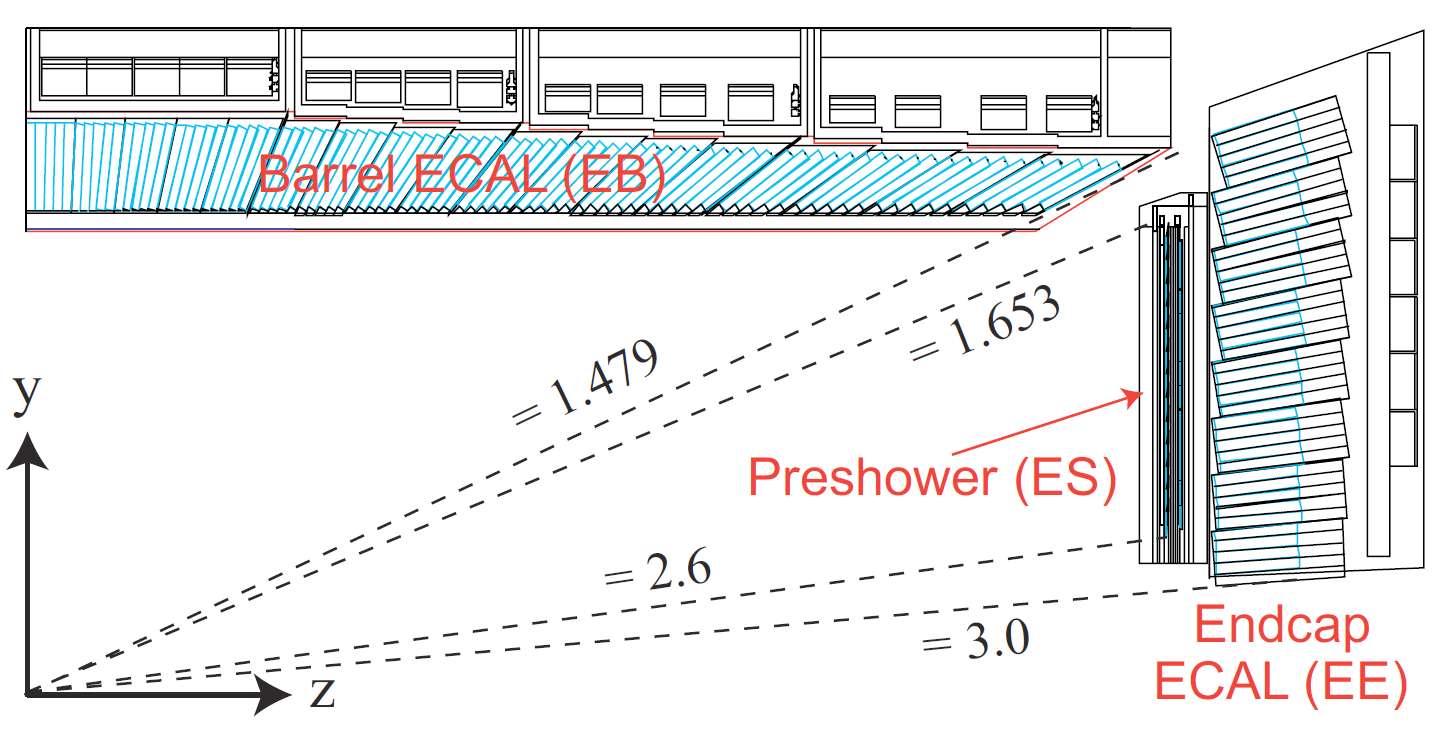
\includegraphics[width=0.8\textwidth]{cms_and_lhc/plots/cms_ecal.png}
     \caption{
Longitudinal view of the CMS detector depicting the ECAL subdetector.
The crystals are inclined towards the interaction region.
     }
     \label{fig:cms_ecal}
\end{figure*}



\subsection{Hadronic Calorimeter}
The hadronic calorimeter(s) (HCAL) provide the necessary energy measurements
to reconstruct charged and neutral hadrons in CMS. These particle are the
primary measurable constituents in ``jets'' and hadronically decay $\tau$
leptons. Additionally, measurement of the energy imbalance from a collision
can indicate the presence of neutrinos or possibly exotic particles~\cite{CMS-Proposal}.
The HCAL is segmented into four calorimeters: the barrel detector, the endcap detector,
the forward hadronic detector, and the barrel outer detector. 
The barrel detector is a sampling calorimeter covering $\abs\eta < 1.3$. It is built
from flat brass absorber plates interleaved with plastic scintillator segments to
measure and readout the deposited energy. The HCAL barrel has coarser granularity
than the ECAL; each segment is $0.087 \times 0.087$ in \etaphi which covers the
same area as 25 ECAL crystals.

The HCAL barrel occupies the space between the ECAL and the superconducting magnet
from a radial distance of 1.77m to 2.95m form the beam line. Particle propagating
outwards at an angle of $\eta = 0$ will encounter the thinnest portion of the
HCAL barrel corresponding to 5.82$\lambda_{l}$. The effective thickness increases
with $\eta$ resulting in 10.6$\lambda_{l}$ at $\abs\eta = 1.3$. The HCAL detector
is depicted in Figure~\ref{fig:cms_hcal}.

To increase the effective
thickness in the barrel region, $\abs\eta < 1.3$, an outer hadronic calorimeter is placed 
outside the superconducting magnet which commplements the barrel calorimeter
extending the effictive thickness to a minimum of 11.8$\lambda_{l}$ in the barrel. 
The HCAL endcap system partially overlapps with the barrel detector and ranges from
$1.3 < \abs\eta < 3.0$.

Beyond $\abs\eta = 3$, the forward hadronic calorimeter, located
11.2m from the interaction point, extend the $\eta$ coverage out to $\abs\eta = 5.2$.
On average, 760\GeV per proton-proton interaction is deposited into the forward 
calorimeters, compared to only 100\GeV for the rest of the detector~\cite{Chatrchyan:2008zzk}.
At higher $\abs\eta$ values, closer to the beam pipe, 
The high particle and radiation flux, at high $\abs\eta$ values, close to the beam pipe,
severly limits the types of detector systems which can survive years of LHC operating
conditions. Because of this, the forward hadronic calorimeter is not the same style sampling
calorimeter like the rest of HCAL. Instead it uses Cherenkov-based, 
radiation-hard, fused-silica quartz fibres embedded in grooves within the steel structure
of the absorber material.

The energy resolution of the HCAL barrel has been measured using test beams~\cite{Elvira:800406}, and is:
\begin{equation}
\label{eqn:hcal_res}
\frac{\sigma}{E} = \frac{115\%}{\sqrt{E/\GeV}} \oplus 5.5\%
\end{equation}
For the forward HCAL system the energy resolution is~\cite{Baiatian:951395},
\begin{equation}
\label{eqn:hcal_res}
\frac{\sigma}{E} = \frac{280\%}{\sqrt{E/\GeV}} \oplus 11\%
\end{equation}
These two equations show the much poorer energy resolution of HCAL compared to ECAL.
There are multiple reasons for this include the fact that the HCAL is a sampling 
calorimter thus much of the energy deposits occure in absorber layers and the 
size of the deposits must be estimated and calibrated for.
Typical HCAL electronics noise $\sigma ^{\text{HCAL}} _{\text{noise}}$ 
is measured to be $\approx$ 200 MeV per tower about 5 times the noise level of
the ECAL barrel crystals, but comparable to the ECAL endcap crystals.

\begin{figure*}[htbp]
\centering
     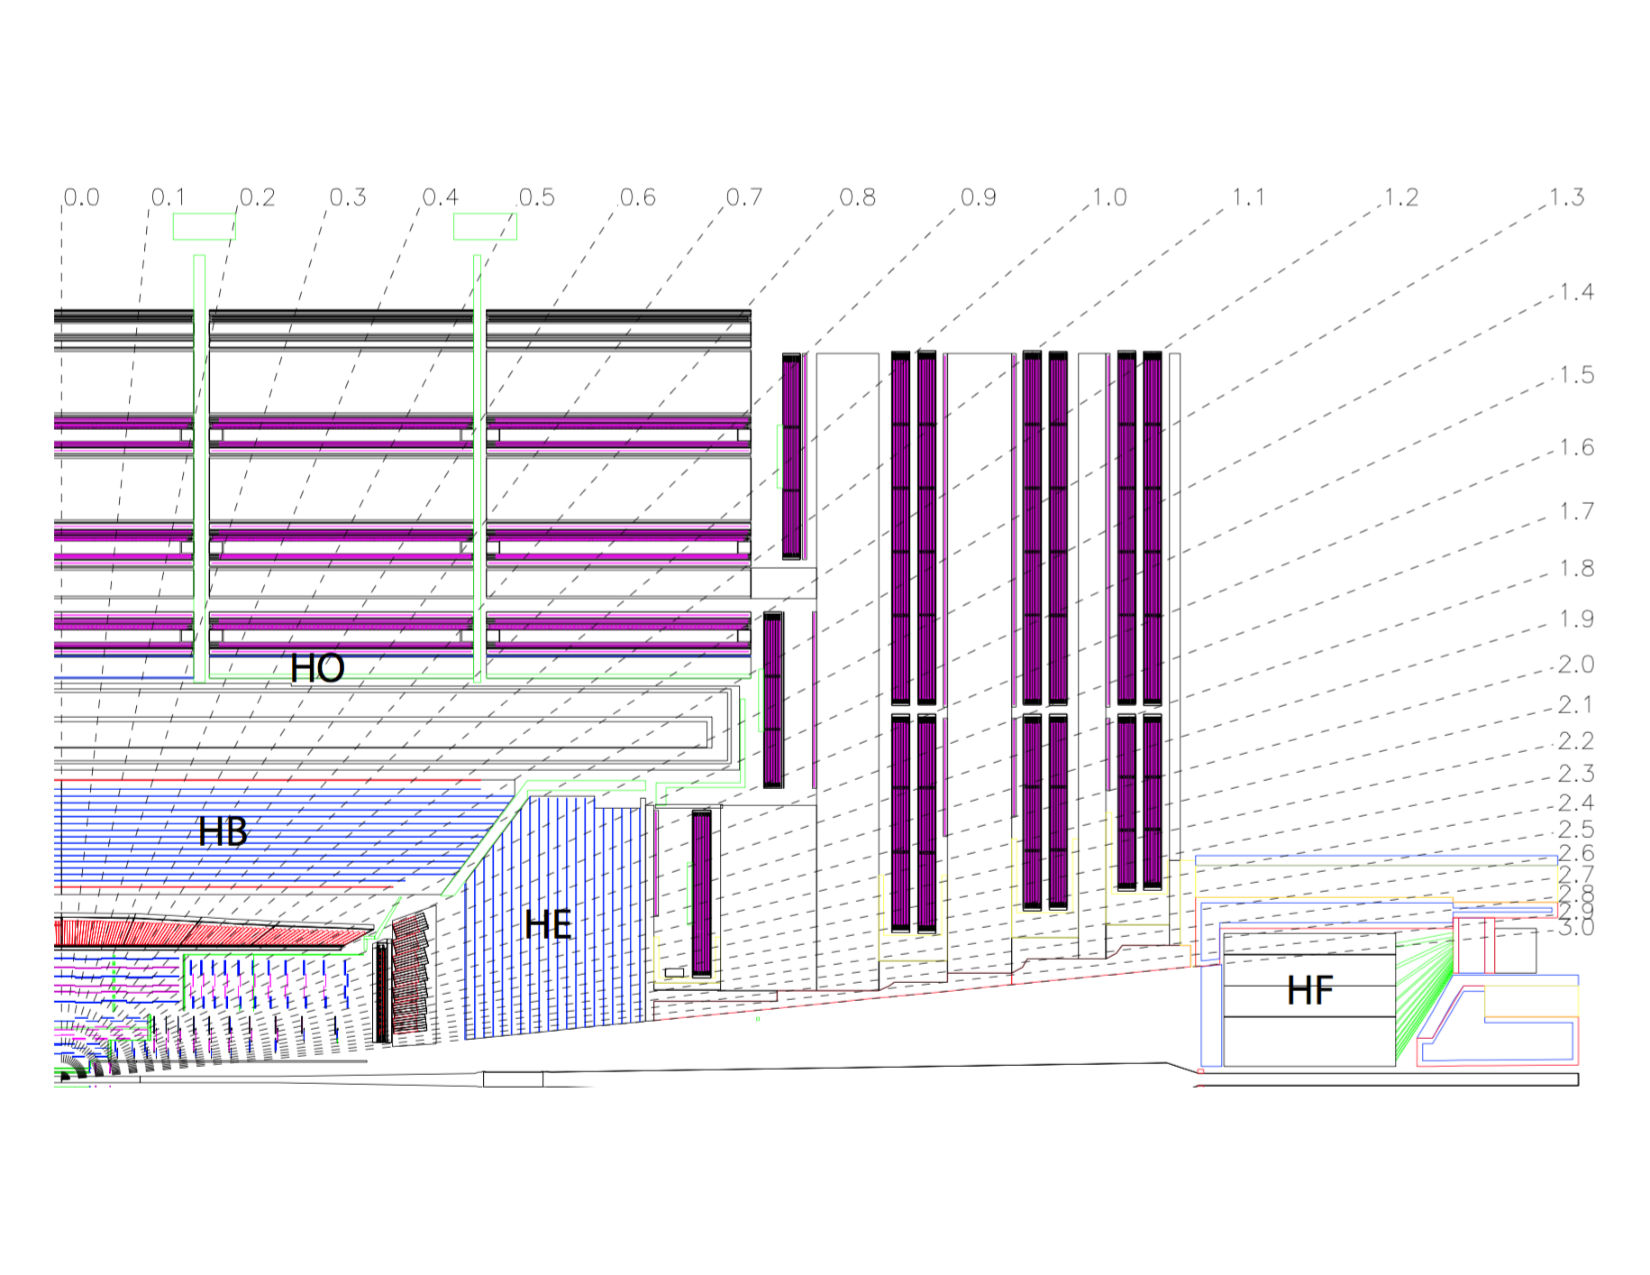
\includegraphics[width=0.8\textwidth]{cms_and_lhc/plots/cms_hcal.pdf}
     \caption{
Longitudinal view of the CMS detector showing the locations of the hadron 
barrel (HB), endcap (HE), outer (HO) and forward (HF) calorimeters. The
effective thickness of the HB detector increases with increasing $\abs\eta$.
     }
     \label{fig:cms_hcal}
\end{figure*}




\subsection{Muon System}
With ``Muon'' in the name of the experiment, it is clear that the muon spectrometer
is important to the physics goals of the CMS experiment. Excellent muon reconstruction, 
identification, and momenutum measurement allows Higgs analyses, such as $\PH \to \PZ\PZ$
where $\PZ\PZ \to \Pgm\Pgm\Pgm\Pgm$ to achieve their most precise mass measurements. Using
2016 data, the $\PH \to \PZ\PZ$ analysis measured the Higgs boson mass with an uncertainty
of approximately 0.2\%, 
$m^{4\Pgm}_{\textrm{H}} = 124.94 \pm 0.25 (\stat) \pm 0.08 (\syst)\GeV$~\cite{cms-2016-hzz}.
In addition to the mentioned functions of the muon system, the high purity of reconstructed
muons makes the system very useful for selecting data events to store.
The muon spectrometer is composed of three subsystems, the drift tubes (DT) which cover
$\abs\eta < 1.2$, the cathode strip chambers (CSC) which cover $0.9 < \abs\eta < 2.4$, and
the resistive plate chambers (RPC) covering $\abs\eta < 1.6$, see Figure~\ref{fig:cms_muon_syst}.

\begin{figure*}[htbp]
\centering
     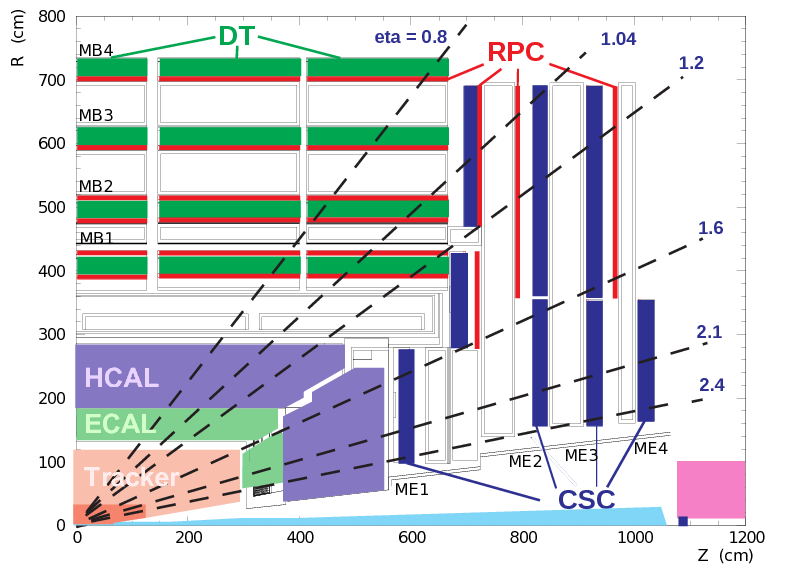
\includegraphics[width=1.0\textwidth]{cms_and_lhc/plots/cms_muon_syst.png}
     \caption{
Layout of one quadrant of CMS. The four DT stations in the barrel (MB1-MB4, green), the four CSC stations in the endcap (ME1-ME4, blue), and the RPC stations (red) are shown.
     }
     \label{fig:cms_muon_syst}
\end{figure*}

The muon subsystems are each embedded within the magnet's flux-return yoke. Each system
detects particles through gas ionization techniques. 
When passing through ionizing gas detectors, charged particles leave a trail of ionized gas 
molecules which can be detected and measured by different techniques.

The drift tubes are used in the barrel region
because of the low expected particle rate and the relatively low strength of the local
magnetic field (which is well contained in the flux-return yoke through the barrel region).
The DTs rely on 172,000 2.4m long sensitive wires maintained at a high voltage to detect the traces
of passing charged particles. The wires are housed in a drift cell with a maximum path length
and time of drift of 21mm and 380ns using a gaseous mixture of 
$85\% \, \textrm{Argon} \, + \, 15\% \, \textrm{CO}_{2}$~\cite{CMS-Proposal}. The drift cell size and drift
time are small enough to avoid high occupancy levels during collisions data taking.
A detailed schmatic of a DT cross-section is in Figure~\ref{fig:cms_muon_dt}.

\begin{figure*}[htbp]
\centering
     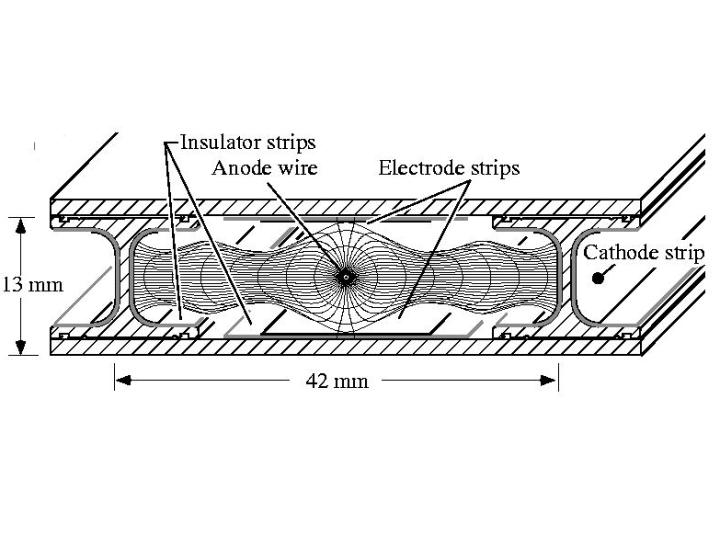
\includegraphics[width=0.7\textwidth]{cms_and_lhc/plots/cms_muon_dt.jpg}
     \caption{
Schematic of a drift tube cell showing drift lines leading to/from the wire 
and isochrones three of which are seen as the concentric lines surrounding the wire. The voltages applied to the 
electrodes are +3600V for wires, +1800V for strips, and −1200V for cathodes.
     }
     \label{fig:cms_muon_dt}
\end{figure*}

Progressing outwards from the barrel region towards higher $\abs\eta$ values, the background 
particle flux increases as does the non-uniformity of the magnetic field in the spacing between
the flux-return yoke. These considerations lead to a different required muon detection technology.
In the two endcap regions of CMS the muon system uses cathode strip chambers arranged as large
disks much like the other subsystem endcaps. The CSCs have a fast 
response time, fine segmentation, and are more radiation resistant than the DTs. The CSC system
is depicted in Figure~\ref{fig:cms_muon_csc} showing the relative arangement of the anode
wires to the cathode strips. The muon coordinate along the anode wires (the $\phi$ coodinate) 
is obtained by interpolating charges induced on strips~\cite{cms-csc}.


\begin{figure*}[htbp]
\centering
     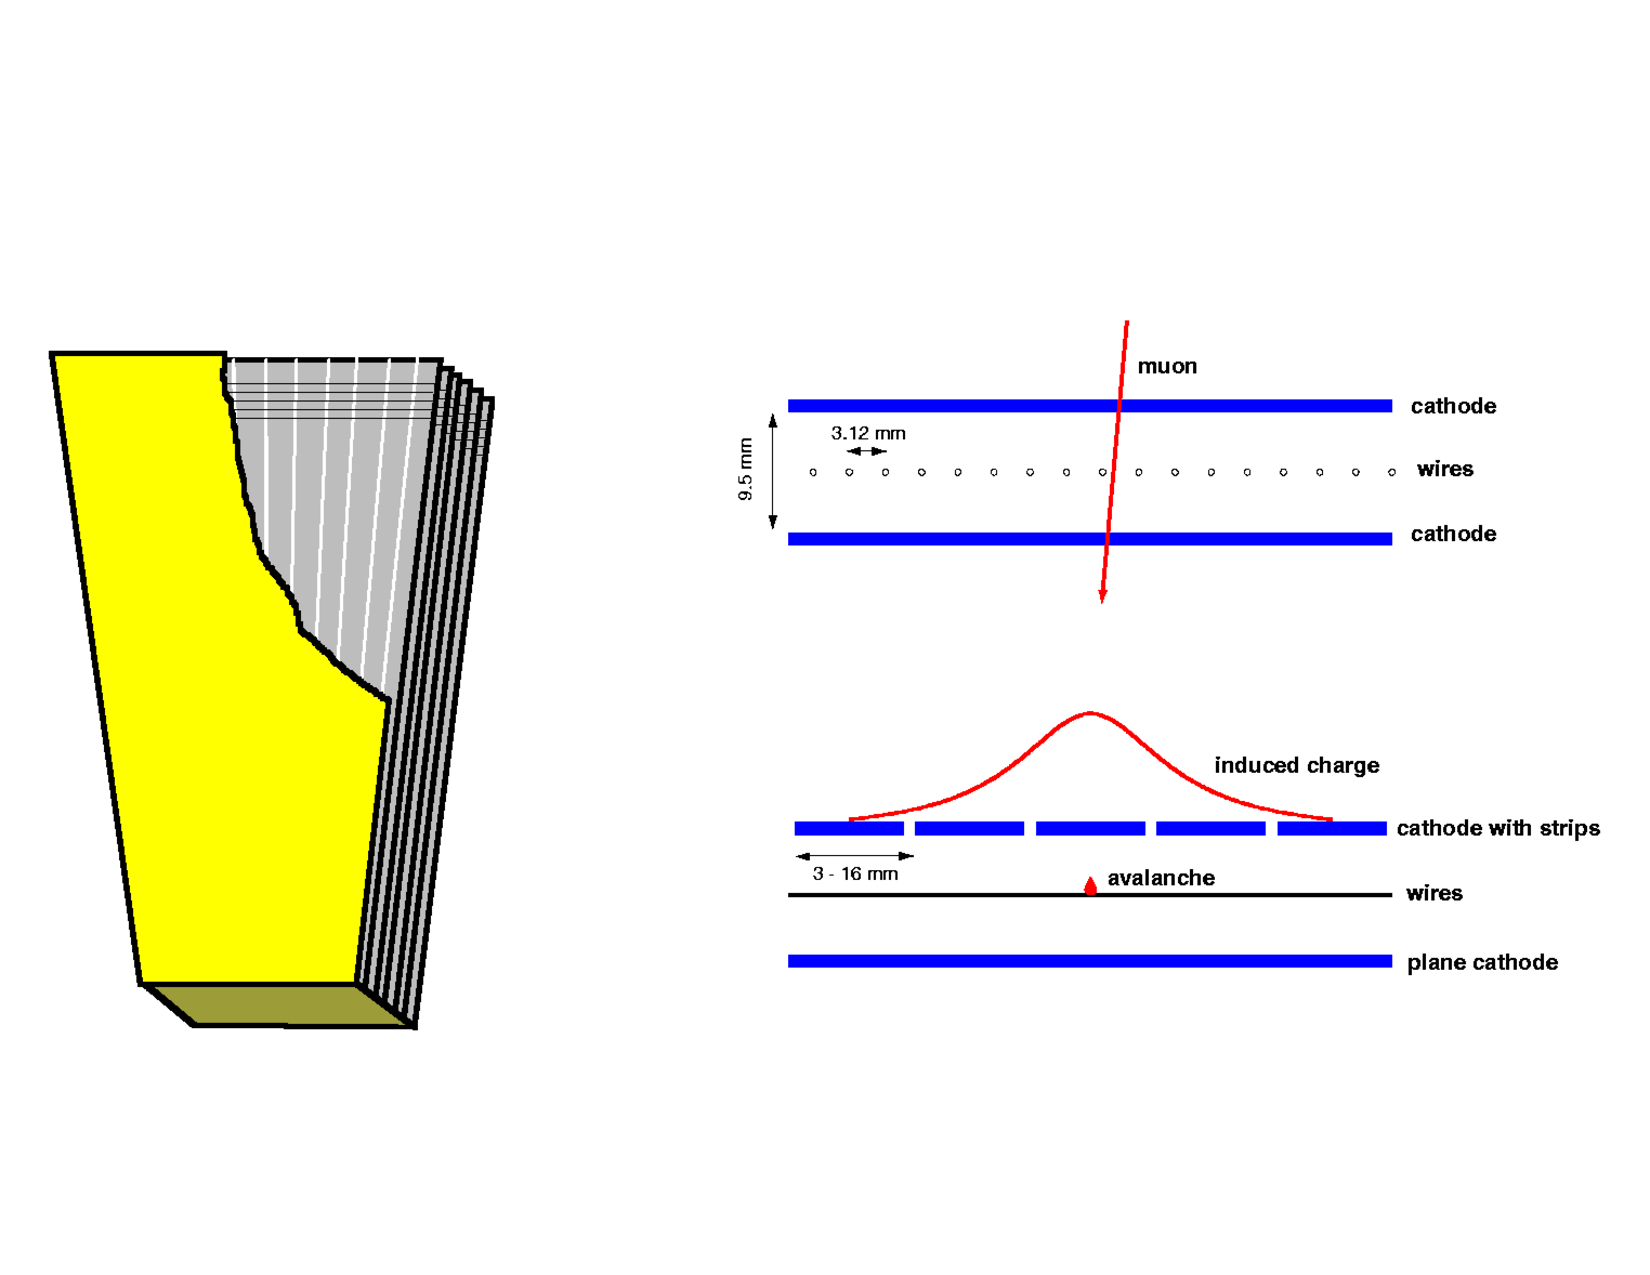
\includegraphics[width=0.8\textwidth]{cms_and_lhc/plots/cms_muon_csc2.pdf}
     \caption{
Schematic of a CSC module composed of 7 trapezoidal panels with 6 gas gaps between
the panels housing the anode wires used to detect the ionized molecules from a passing
muon. The cut-out in the top panel shows the anode wires running horizontally and 
the cathode strips running vertically.
     }
     \label{fig:cms_muon_csc}
\end{figure*}


Because of the uncertainty in the eventual background rates and in the ability of the muon system to measure the correct beam-crossing time when the LHC reaches full luminosity, a com- plementary, dedicated trigger system consisting of resistive plate chambers (RPC) was added in both the barrel and endcap regions. The RPCs provide a fast, independent, and highly-segmented trigger with a sharp pT threshold over a large portion of the rapidity range (|η| < 1.6) of the muon system. The RPCs are double-gap chambers, operated in avalanche mode to ensure good operation at high rates. They produce a fast response, with good time resolution but coarser position reso- lution than the DTs or CSCs. They also help to resolve ambiguities in attempting to make tracks from multiple hits in a chamber.~\cite{1748-0221-8-03-T03001}.



\subsubsection{Drift Tubes}
\subsubsection{Cathode Strip Chambers}
\subsubsection{Resistive Plate Chambers}
\subsection{Trigger and Data Acquisition}
40 MHz - high speed electronics capable of operating in close synchronization
trigger, L1, HLT
Significant upgrades of the L1 trigger during the first long shutdown of the LHC have benefitted this analysis, especially in the $\tauh\tauh$ channel. These upgrades improved the $\tauh$ identification at L1 by giving more flexibility to object isolation, allowing new techniques to suppress the contribution from additional $\Pp\Pp$ interactions per bunch
crossing, and to reconstruct the L1 $\tauh$ object in a fiducial region that matches more closely that of a true hadronic $\Pgt$ decay. The flexibility is achieved by employing high bandwidth optical links for data communication and large field-programmable gate arrays (FPGAs) for data processing.

\subsubsection{Level-1 Trigger}
\subsubsection{Aside for CaloL1 Duties and Online SW}
\subsubsection{HLT}
\subsubsection{Aside for 2018 Tau Trigger Updates}
\subsubsection{Aside for Phase-2 L1EG Discussion}

%\chapter{Simulation}
\label{sec:simulation}

Signal and background processes are modeled with samples of simulated events.
The signal samples with a Higgs boson produced through gluon fusion ($\cPg\cPg\PH$), vector boson fusion (VBF),
or in association with a $\PW$ or $\PZ$ boson ($\PW\PH$ or $\PZ\PH$), are generated at next-to-leading order (NLO) in perturbative quantum chromodynamics (pQCD) with the \POWHEG 2.0~\cite{Nason:2004rx,Frixione:2007vw, Alioli:2010xd, Alioli:2010xa, Alioli:2008tz} generator. The \textsc{minlo hvJ}~\cite{Luisoni:2013kna} extension of \POWHEG 2.0 is used for the $\PW\PH$ and $\PZ\PH$ simulated samples. The set of parton distribution functions (PDFs) is NNPDF30\_nlo\_as\_0118~\cite{Ball:2011uy}. The $\ttbar\PH$ process is negligible.
The various production cross sections and branching fractions for the SM Higgs boson production, and their corresponding uncertainties are taken from Refs.~\cite{deFlorian:2016spz,Denner:2011mq,Ball:2011mu} and references therein.

The \aMCATNLO~\cite{Alwall:2014hca} generator is used for $\PZ+$jets and $\PW+$jets processes. They are simulated at leading order (LO) with the MLM jet matching and merging~\cite{Alwall:2007fs}.
The \aMCATNLO generator is also used for diboson production simulated at next-to-LO (NLO) with the FxFx jet matching and merging~\cite{Frederix:2012ps}, whereas \POWHEG 2.0 and 1.0 are used for $\ttbar$ and single top quark production, respectively.
The generators are interfaced with \PYTHIA 8.212 ~\cite{Sjostrand:2014zea} to model the parton showering and fragmentation, as well as the decay of the $\Pgt$ leptons.
The \PYTHIA parameters affecting the description of the underlying event are set to the {CUETP8M1} tune~\cite{Khachatryan:2015pea}.

Generated events are processed through a simulation of the CMS detector based on
GEANTfour~\cite{Agostinelli:2002hh}, and are reconstructed with the same algorithms used for data.
The simulated samples include additional $\Pp\Pp$ interactions per bunch
crossing, referred to as ``pileup''.
The effect of pileup is taken into account by generating concurrent minimum bias collision events generated with \PYTHIA.
The simulated events are weighted such that the distribution of the number of additional pileup interactions, estimated from the measured instantaneous luminosity for each bunch crossing, matches that in data, with an average of approximately 27 interactions per bunch crossing.

\section{Hard Scattering Process}
\section{Monte Carlo Generator Programs}
\section{Detector Simulation}



%\chapter{Object Reconstruction and Selection}

In this chapter I discuss the progression from detector-based signals through to an
overall event reconstruction within CMS. At CMS, physics-object reconstruction draws
on input from all detector subseystems simultaneously to build particle tracks
and cluster together energy deposits, to link together these tracks and energy
deposits to construct basic physics-objects such as electrons and charged
hadrons, and to build composit objects such as ``jets'' and hadronically decaying
$\tau$ leptons. Event based quantities such as the \etvecmiss are also reconstructed.
To achieve all of this, CMS uses its Particle Flow (PF) reconstruction 
algorithm~\cite{Sirunyan:2017ulk}. The particle flow concept has been used in the 
past by other experiments such as ALEPH at LEP~\cite{PF-ALEPH}. CMS is the first
experiment to fully utilize the particle flow techinque in a hadron collider environment.
A discussion of the reconstruction of the two basic PF objects, tracks and energy
clusters, follows in the next section. Afterwards I detail the construction of 
the PF physics-objects then move to the composit objects and full event variables.
The PF approach allows particles from pileup interactions to be identified 
and enables efficient pileup mitigation methods.

\section{Particle Flow Input}
The CMS detector and the PF reconstruction algorithm were specifically designed to
compliment eachother. The CMS detector features: a highly-segmented tracker well
suited to track reconstruction, a fine-grained electromagnetic calorimeter necessary
to separate the individual energy deposits from particles within ``jets'' and
efficient photon and electron identification, a hermetic hadron 
calorimeter for the measurement and identification of charged and neutral hadrons, 
a strong magnetic field for the measurement of the momenta of charged particles and to
separate the calorimeter energy deposits of charged and neutral hadrons within ``jets'', and 
an excellent muon spectrometer for muon identification and to disintangle the muon
tracks from other tracks in the tracker. A schematic of a slice of the CMS detector
and different physics-objects transversing the detector subsystems can be see in
figure~\ref{fig:cms_slice}. The different detector systems all contribute
necessary pieces of information to the PF reconstruction. From the raw detector
signals two classes of PF objects are created, tracks and energy clusters.

\begin{figure*}[htbp]
\centering
     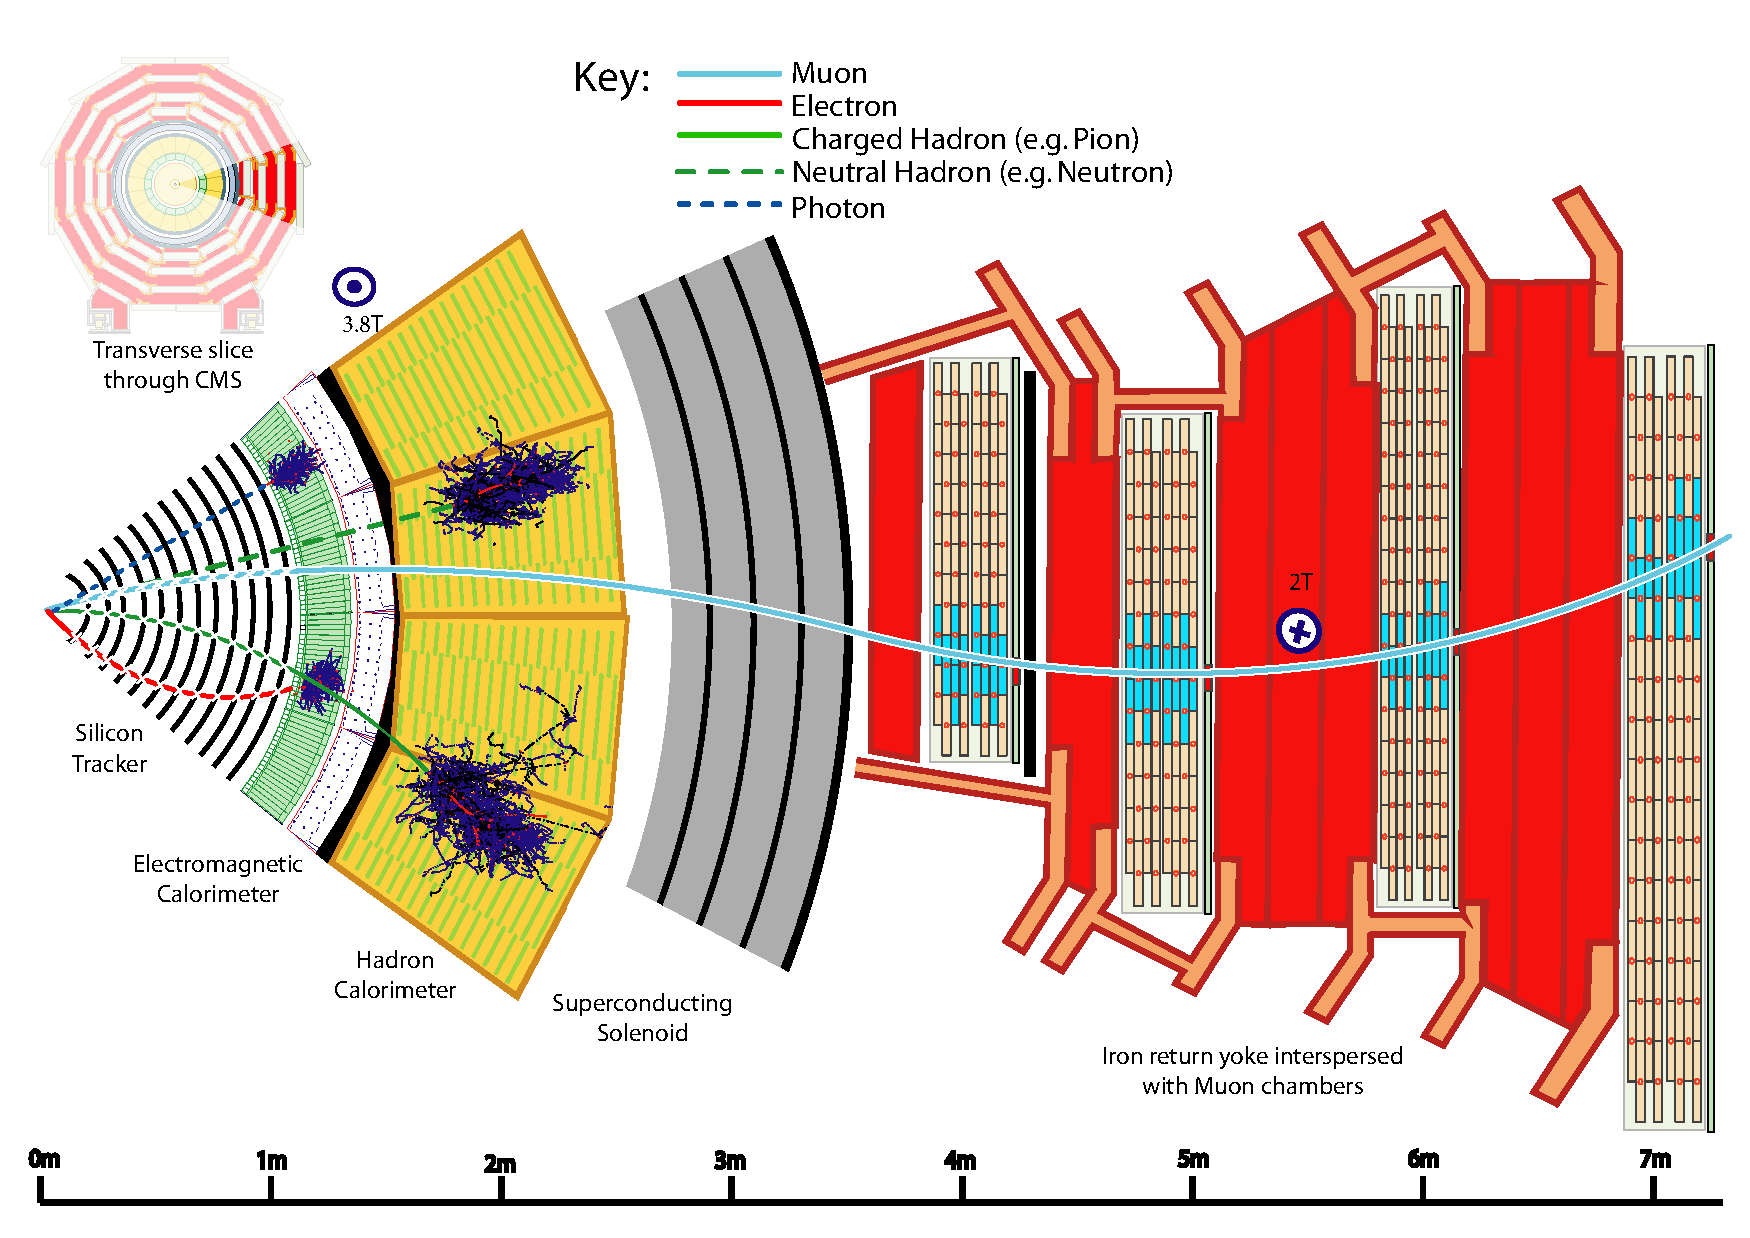
\includegraphics[width=1.0\textwidth]{object_reconstruction_and_selection/plots/cms_slice.pdf}
     \caption{
A schematic of a slice of an x-y cross section of the CMS detector showing different
physics-objects such as electrons, photons, charged and neutral hadroncs, and muons
propagating outwards from the collision region within the detector. The schematic
shows how tracks are linked to energy deposits and in which subdetector regions different
particles deposit most of their energy on average.
     }
     \label{fig:cms_slice}
\end{figure*}


\subsection{Particle Flow Tracks}
Energy deposits often called ``hits'' are recorded by the pixel and strip tracks during
a collision. From these, charged particle tracks are reconstructed in subsequent layers
mapping the progression of charged particles from the beam axis outwards into the detector
volume. Attempting to reconstruct tracks from every possible hit combination quickly
because unreasonable considering the over 70 million tracker pixels and strips which can
each record a hit. PF uses a combinatorial track finder based on Kalman 
Filtering (KF); the algorithim is broken down into three successive steps.
\begin{itemize}
\item Generate seed tracks from a few hits which are compatible with a charged
particle trajectory
\item Gathering other hits along the seed track trajectory when propagated through
the rest of the tracker subsystem
\item Final track fitting to determine track properties such as the origin, transverse
momentum, and direction.
\end{itemize}
Only tracks meeting certain quality standards are kept for analysis. These tracks must
be seeded with two hits in consecutive layers in the pixel detector, and are required 
to be reconstructed with at least eight tracker hits in total, and with at most one 
missing hit along the track trajectory. Tracks must also have a curvature corresponding
to a momentum greater than 0.9\GeV.

There is a balance that must be struck between imposing tight quality cuts on reconstructed
tracks which increases the purity of genuine track within the reconstructed track collection
but also decreases the efficiency for reconstructing genuine tracks, and loosening
quality cuts to reconstruct genuine tracks with a higher efficiency and lower purity.
After an initial pass through what is called the global combinatorial track finder,
which has stringent track quality criteria impossed by the eight hit requirement, 
the efficiency to reconstruct
genuine tracks is roughly 80\% for charged pions with $\pt = 10\GeV$, and 99\%
for isolated muons. This corresponds to a misreconstructed track rate in the range of
about 2.5\% for charged pions with $\pt = 10\GeV$, see figure~\ref{fig:kf_tracking}.
As hits are recorded in a reconstructed track, they are removed from the available,
unused hits which can be combined in subsequent passes through the tracking algorithm.

There are ten passes through the tracking algorithm in total. Each pass loosens the track quality criteria,
such as $\chi^2$ and number of hits requirements, beyond the stingent initial criteria.
This helps to reconstruct difficult to build tracks. Tracks can be difficult to 
reconstruct for multiple reasons such as detector inefficiencies leading to missing
detector hits, or particles originating from elsewhere in the detector 
besides along the beam axis. These tracks could be from hadrons interacting
within the tracker material before reaching the eight-hits threshold, or from the decay
of particles with finite life-times. Additionally, there can be difficulty disintangling
the many tracks within a collimated ``jet'' where many of the tracks are close to or
nearly overlapping with one another.
The misreconstruction rate is suppressed in each iterative step despite the loosening
quality criteria by the removal of the hits which are previously incorporated into
a reconstructed track. This  suppresses the random hit-to-seed association in the
next iteration and allows moderate efficiency gains for only small misreconstruction losses.
The efficiency and misreconstruction rate in figure~\ref{fig:kf_tracking} shows the
results for the initial pass throug the tracking algorithm, the results after all
passes which require the track seed to contain hits in the pixel detector, and the
final results after considering displaced tracks as well.
After all iterations the efficiency is about 90\% for a charged pions with $\pt = 10\GeV$
for a misreconstruction rate of 3\%.

\begin{figure*}[htbp]
\centering
     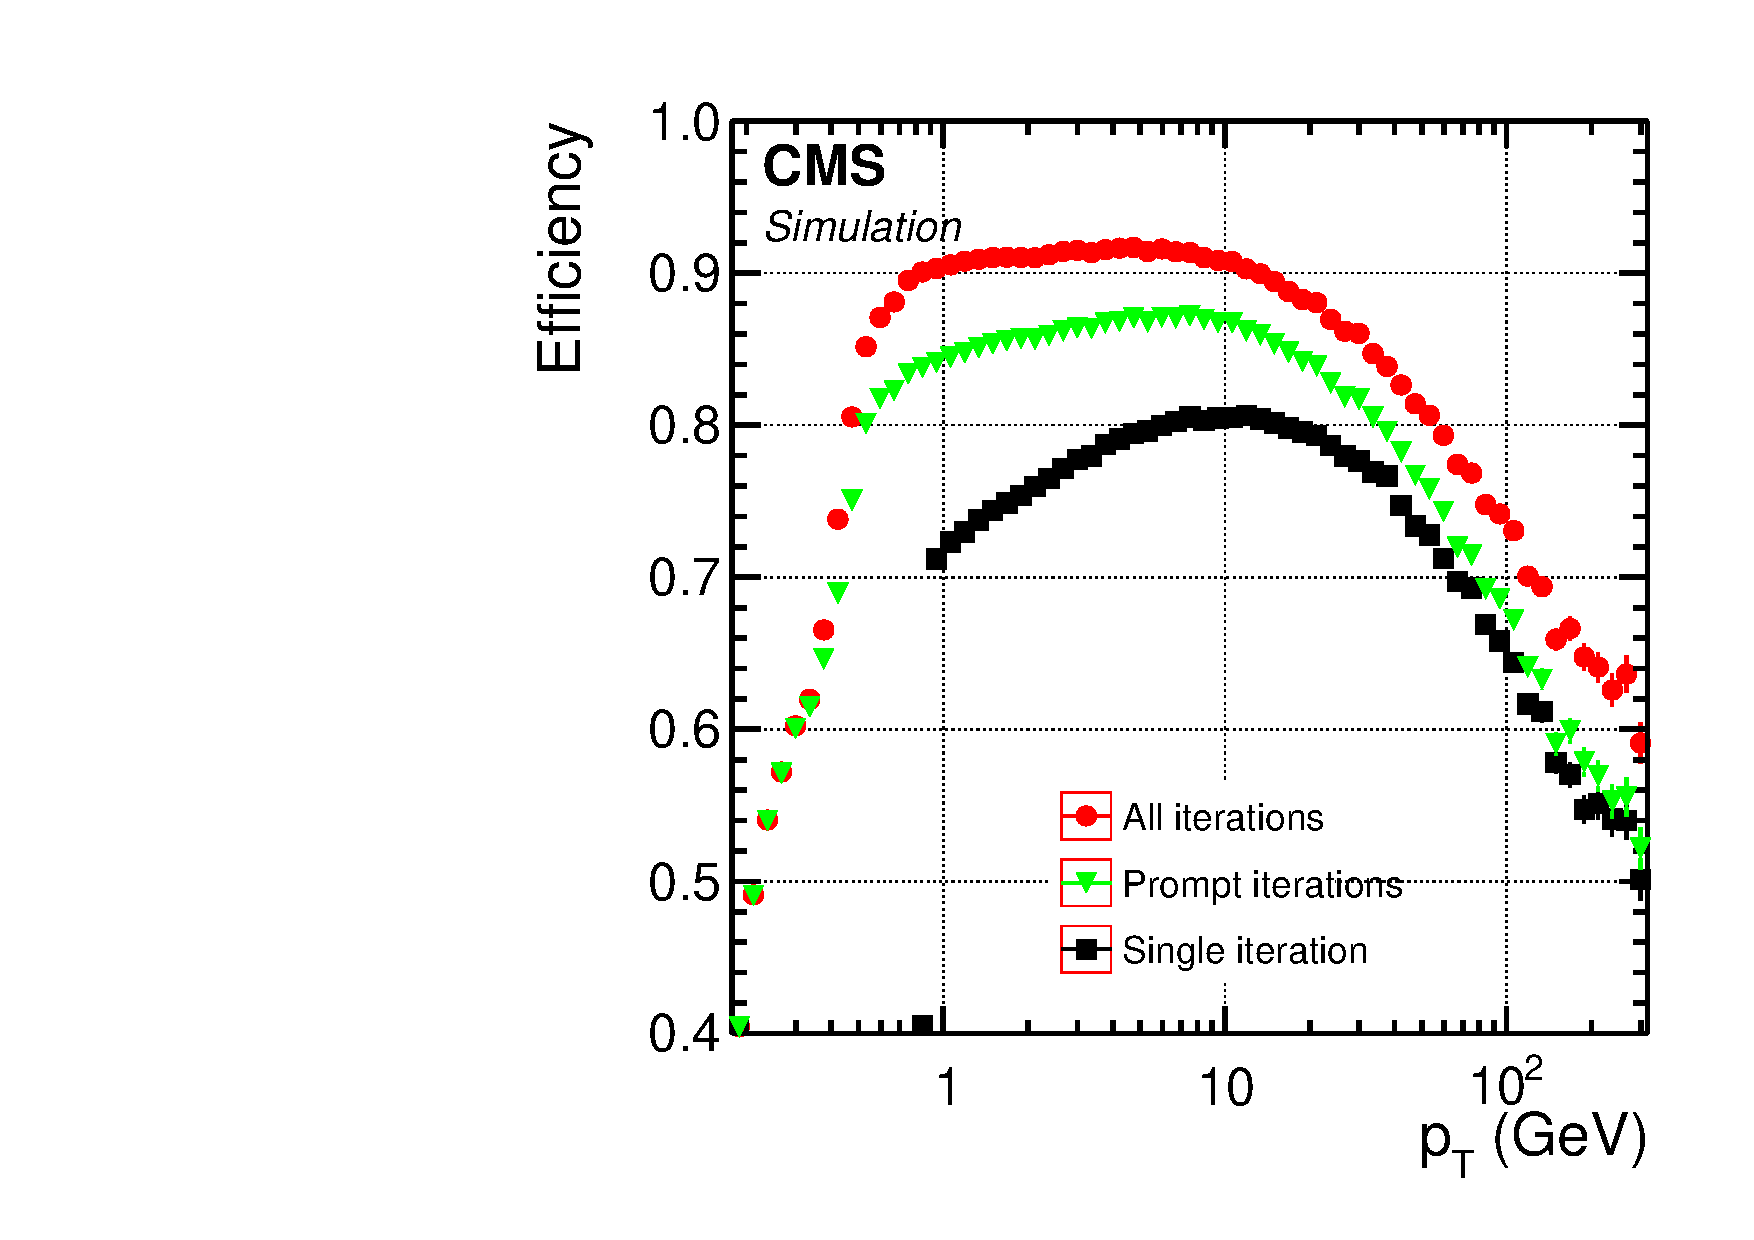
\includegraphics[width=0.45\textwidth]{object_reconstruction_and_selection/plots/pf_track_eff.pdf}
     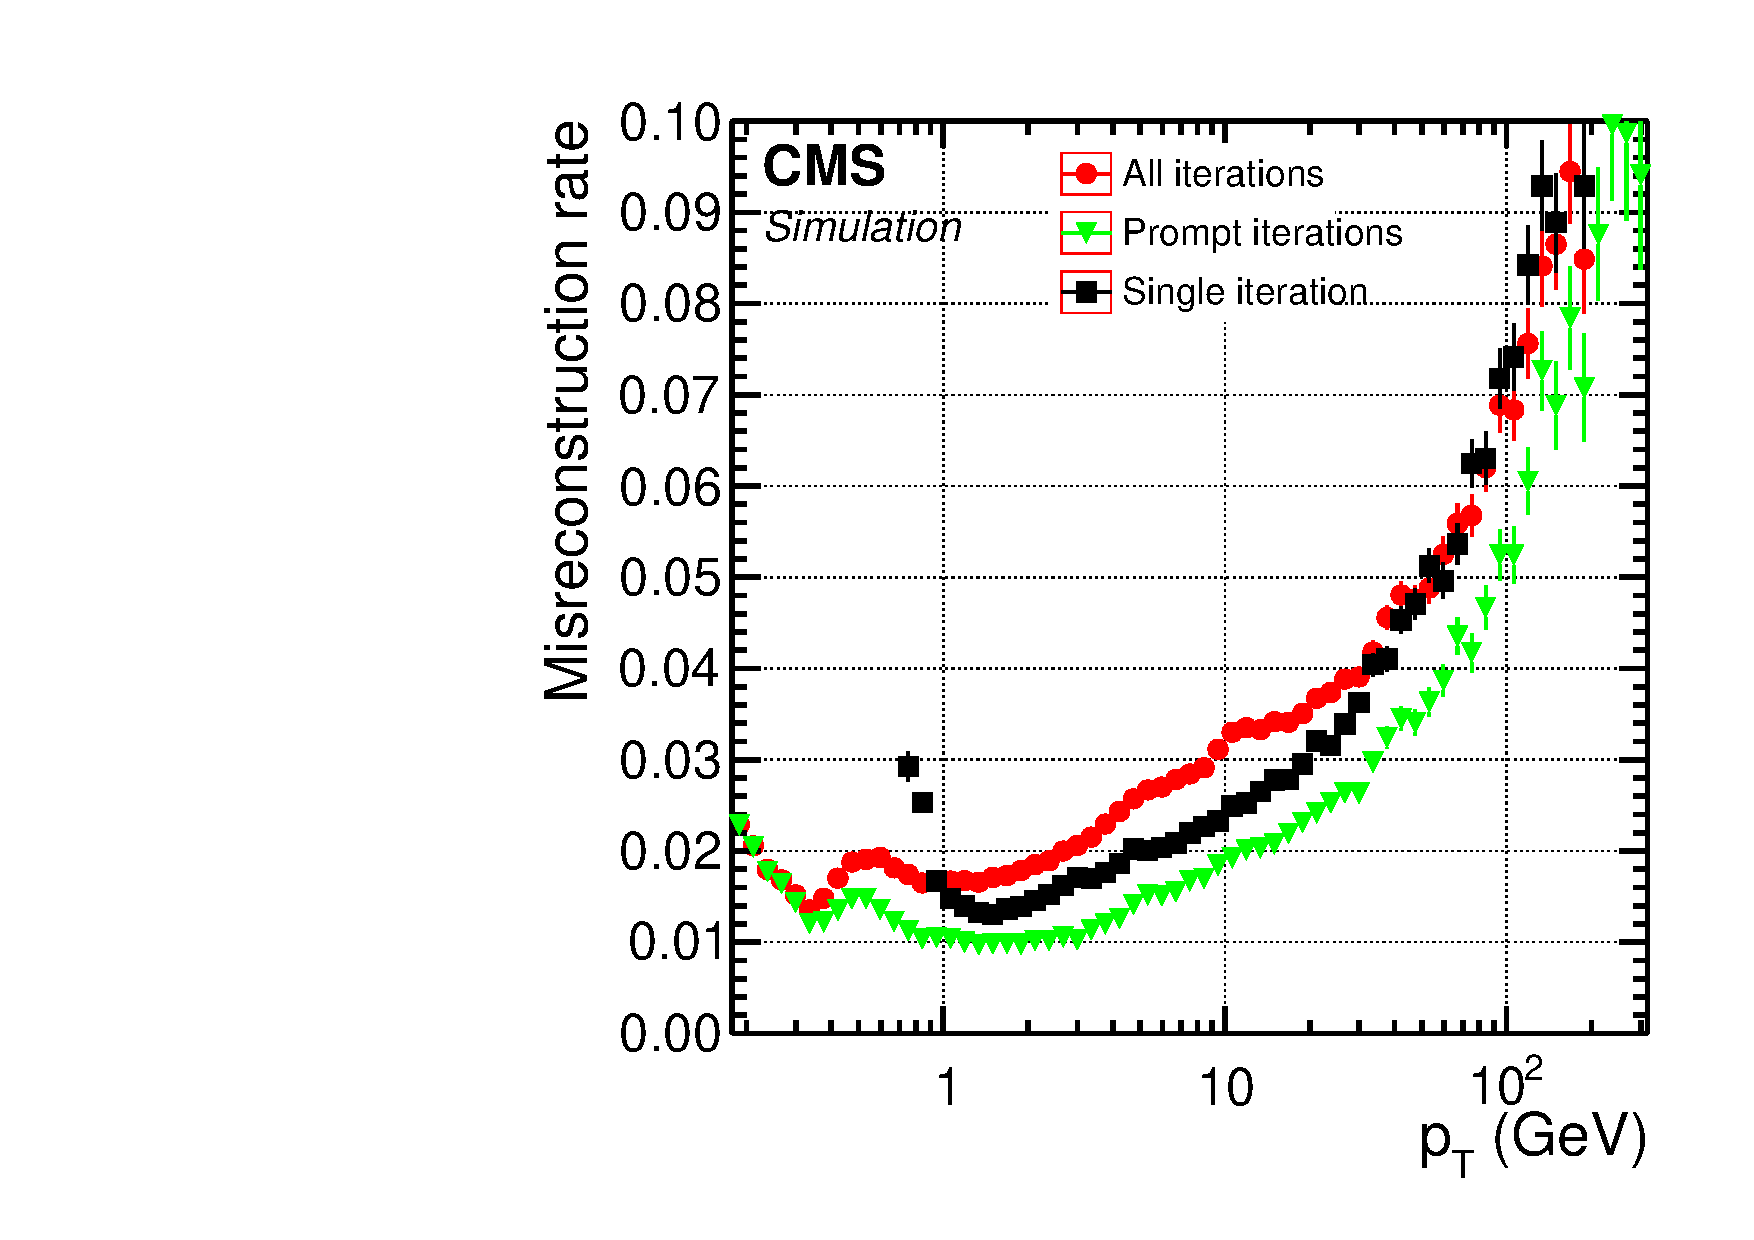
\includegraphics[width=0.45\textwidth]{object_reconstruction_and_selection/plots/pf_track_misId.pdf}
     \caption{
Efficiency (left) and misreconstruction rate (right) of the global combinatorial track finder (black squares) 
which is the first pass through the tracking algorithm. The prompt iterations of the tracking method (green 
triangles) show the results after all iterations based on seeds with at least one 
hit in the pixel detector are completed. The final results after all iterations (red circles) includes
iterations with displaced seeds. Efficiency and misreconstruction are plotted as a function 
of the track $\pt$, for charged hadrons in multijet events without pileup interactions. Only tracks with 
$\abs\eta < 2.5$ are considered. The efficiency 
is displayed for tracks originating from within 3.5 cm of the beam axis and $\pm$30 cm of the nominal 
centre of CMS along the beam axis.
     }
     \label{fig:kf_tracking}
\end{figure*}

Tracks which are likely associated with electrons receive special treatment in PF. Electrons
will often emit bremsstrahlung radiation while propagating through the tracker making their
tracks difficult to reconstruct because of the sudden kinks. 
When energetic photons are radiated from an electron, the pattern recognition in the KF algorithm
may have difficulty accommodating the sudden change in electron momentum. This can cause the track to 
be reconstructed with a small number of hits than would be associated with the true electron
path. A new collection of tracks is created based on a preselection on the number of hits and 
the fit $\chi^2$ for the reconstructed KF-based tracks. The new collection which is a subset of the
KF-based tracks are fit again with a Gaussian-sum filter (GSF)~\cite{gsf_electrons}. Instead of
modeling the energy loss of particles as a single gaussian probability density function (PDF) like the KF
algorithm does, the GSF models the energy loss as a mixture of multiple gaussiand PDFs. 
The GSF fitting algorithm is more adapted to electrons than the KF used in the iterative tracking.
It allows for sudden and substantial energy losses along the trajectory. The
additional freedom here allows much better fits for the electron-based tracks and provides
better estimates for the track origin, trajector towards the calorimeters, and $\pt$.

Muon tracks are built from a combination of the pixel and strip tracker information and the
muon spectrometer information. High purity muon hits in the muon spectrometer is granted by the 
calorimeters and the solenoid which absorb the vast majority of non-muon particles, except neutrinos, 
before reaching the muon spectrometer. There are three difference categories of muon tracks
reconstructed:
\begin{itemize}
\item Standalone muons are based on hits within each DT or CSC detector. Hits are clustered to form 
track segments that are used as seeds for the pattern recognition in the muon spectrometer to gather
other hits in the muon systems along the muon trajectory.
\item Global muons are reconstructed from a standalone-muon track which is matched to a track 
in the inner tracker. If the trajectory parameters of the two tracks propagated onto a common surface 
they are considered compatible and the hits from the inner track and from the standalone-muon track are combined and fit to form a global-muon track.
\item Tracker muons are built from an extrapolation of a track from the inner track system to a
single compatibe muon segment within the muon spectrometer system. The inner tracker-based track must have 
a $\pt > 0.5\GeV$ and a total momentum p in excess of 2.5 GeV.
\end{itemize}

About 99\% of the muons produced within the geometrical acceptance of the muon system are 
reconstructed either as a global muon or a tracker muon and very often as both.
For muons with $\pt > 200\GeV$ the momentum resolution, based on the inner track, is 
improved by the inclusion of the track extension to the muon system.
For muons with $\pt < 200\GeV$ the inner tracker already provides a precise measurement of 
their momentum.



\subsection{Particle Flow Energy Clusters}
Energy clusters make up the second basic building block to construct PF physics-objects. The PF energy
clustering algorithm which constructs the energy clusters serves multiple purposes. The energy clustering
is designed to:
\begin{itemize}
\item Detect and measure the energy and direction of stable neutral particles (photons and neutral hadrons)
\item Separate neutral particles from charged hadron energy deposits
\item Reconstruct and identify electrons and all accompanying bremsstrahlung photons
\item Assist the energy measurement of charged hadrons for which the track parameters were not 
determined accurately; this is primairly the case for low-quality and high-$\pt$ tracks
\end{itemize}
The clustering is performem separately in each subdetector, the ECAL barrel and end caps and HCAL barrel
and end caps with an aim of a high detection efficiency even for low-energy particles and the ability to 
separat close energy deposits. Clustering begins with seed hits which have an energy above the seed hit
threshold and an energy larger than the energy of the adjacent hits. In the ECAL barrel, the fine 
granularity of the ECAL allows
for the clustering to consider all eight adjacent hits, four on the sides and four on the corners.
The HCAL barrel has a more coarse granularity, so only the four adjacent sides are considered when
selecting a seed candidate. From the starting seed, topological clusters are grown outward by aggregating
hits with at least a corner in common with a cell already included in the cluster. Hits must have an energy
in excess of two times the subdetector noise level to be considered for clustering. The energy thresholds
for seeding a cluster and cluster inclusion threshold are in table~\ref{tab:pf_cluster_thresholds}.


\begin{table*}[htbp]
\centering
\begin{footnotesize}
%\begin{scriptsize}
\begin{tabular}{|l|cc|cc|}
\hline
        &       \multicolumn{2}{|c|}{ECAL}        &       \multicolumn{2}{|c|}{HCAL}        \\  %&   Preshower \\
        &   barrel  &   endcaps        &       barrel   &   endcaps        \\  %&    \\
\hline
Cell $E$ threshold (\MeV) & 80 & 300    &   800 &   800 \\   %& 0.06 \\
\hline
Seed Number closest cells   &   8 & 8   &   4 & 4 \\    %& 8 \\
Seed $E$ threshold (\MeV)   &  230  &  600  &  800  & 1100 \\    %& 0.12  \\
Seed $E_{\text{T}}$ threshold (\MeV)   &  0  &  150  & 0   & 0 \\    %& 0 \\
%\hline
%Gaussian width (cm)   &  1.5  &  1.5  &  10.0  & 10.0  \\    %& 0.2 \\
\hline
\end{tabular}
\end{footnotesize}
%\end{scriptsize}
\label{tab:pf_cluster_thresholds}
\caption{
The clustering parameters used for ECAL and HCAL energy deposit clustering. The ECAL endcap
requires an additional seed $E_{\text{T}}$ threshold because the detector noise
increases as a function of $\abs\eta$.
}
\end{table*}

Residual energy calibrations are applied to the ECAL and HCAL energy clusters. The calibrations are
designed to account for the effects of the hit energy thresholds which will always result in a 
smaller amount of energy being incorporated into a cluster than was measured by the detector
for a given single object.
In the ECAL, the residual energy calibration is determined from simulated single photon events.
This generic calibration is applied to all ECAL clusters prior to the hadron cluster calibration 
mentioned next. 

ECAL and HCAL energy clusters are linked together as a potential hadronicy decay energy deposit
if their positions in \etaphi overlap. For a hadronic decay, the total calorimeter response (ECAL + HCAL) depends on 
the fraction of the shower energy deposited in the ECAL, and is not linear with energy. The 
ECAL and HCAL cluster energies therefore need to be substantially recalibrated to get an 
estimate of the true hadron energy. Simulated single neutral hadrons, specifically single 
$\text{K}^{0}_{\text{L}}$s, are used for the hadronic decay response calibration seen for the
barrel in figure~\ref{fig:pf_calo_calib}. The applied calibrations in the left plot lead
to excellent agreement in the calorimeter response in the right plot. It is much harder to
make larger improvements in the energy resolution without actually changing the available
input calorimeter hit information granularity.


\begin{figure*}[htbp]
\centering
     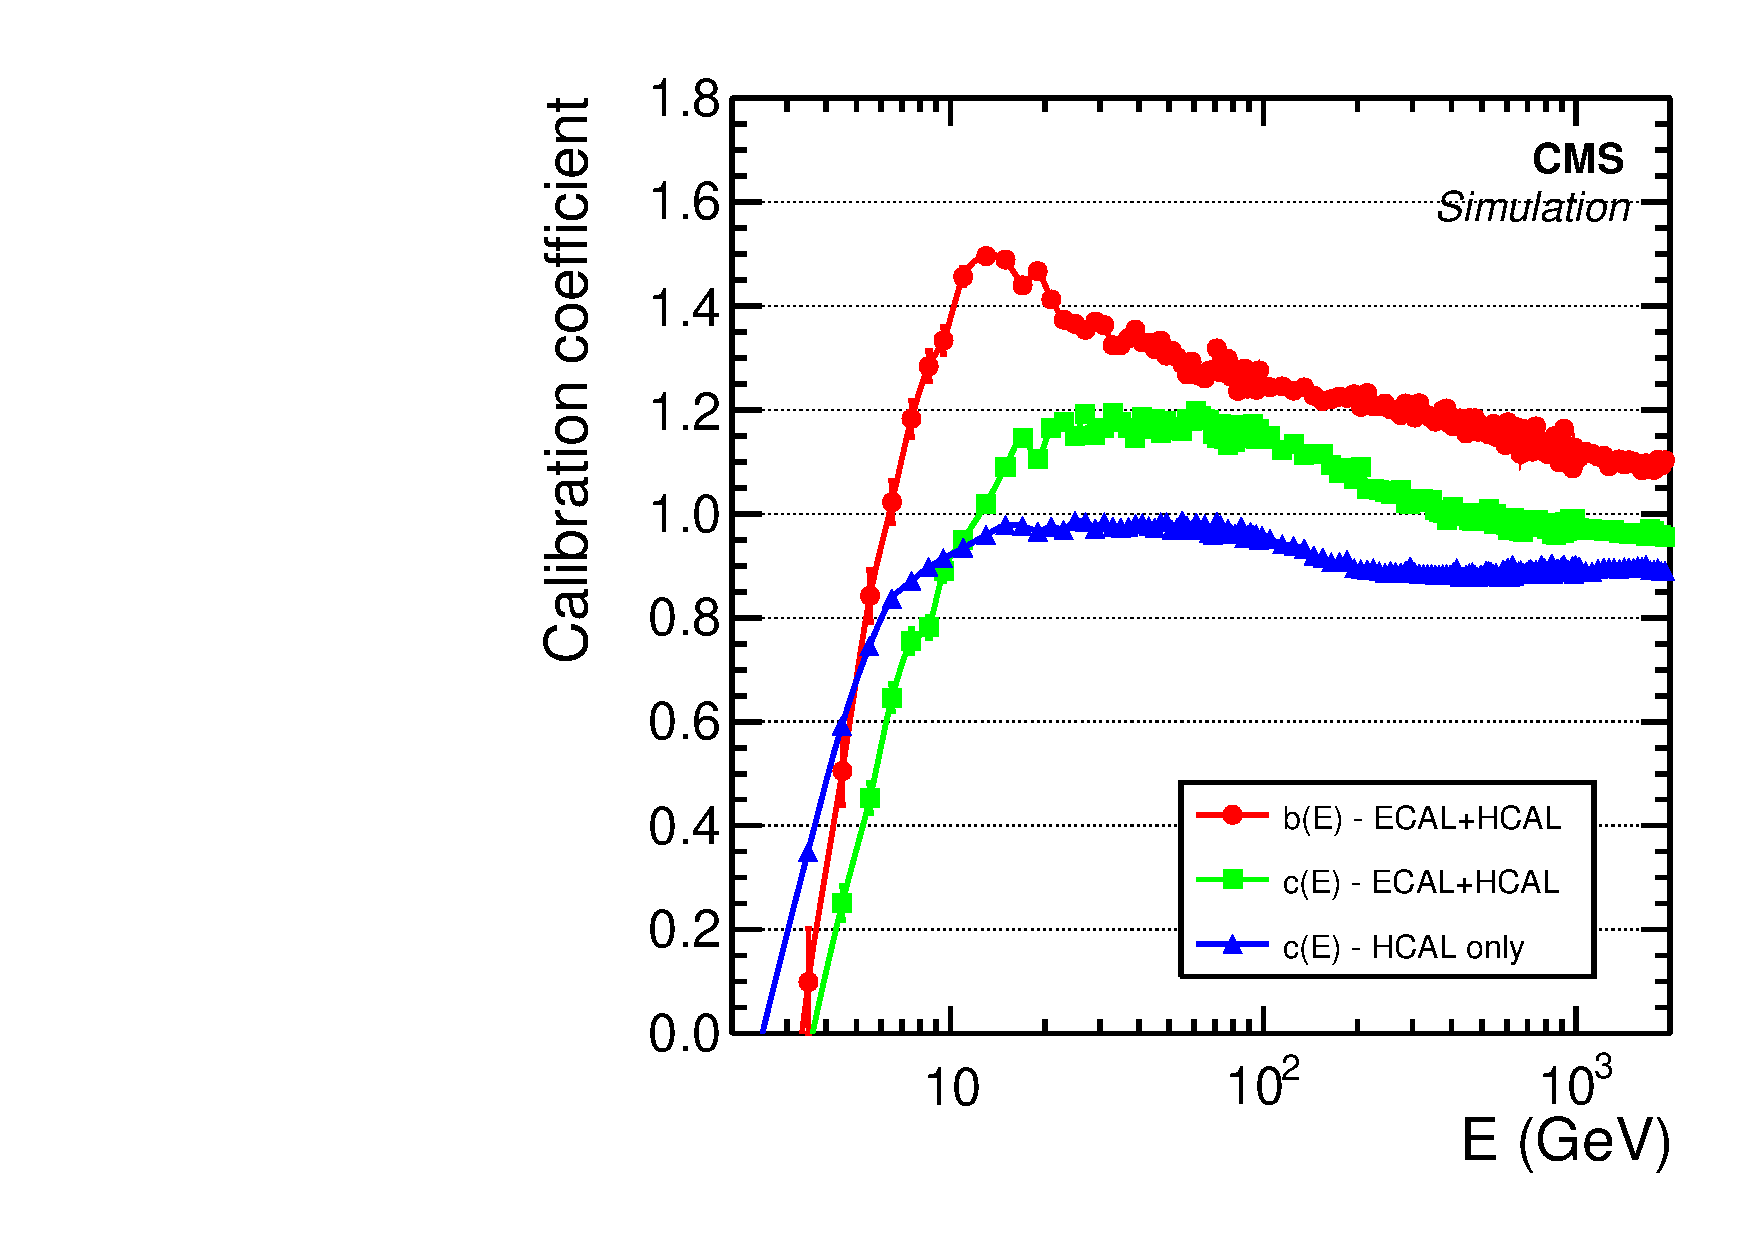
\includegraphics[width=0.45\textwidth]{object_reconstruction_and_selection/plots/calo_calibrations.pdf}
     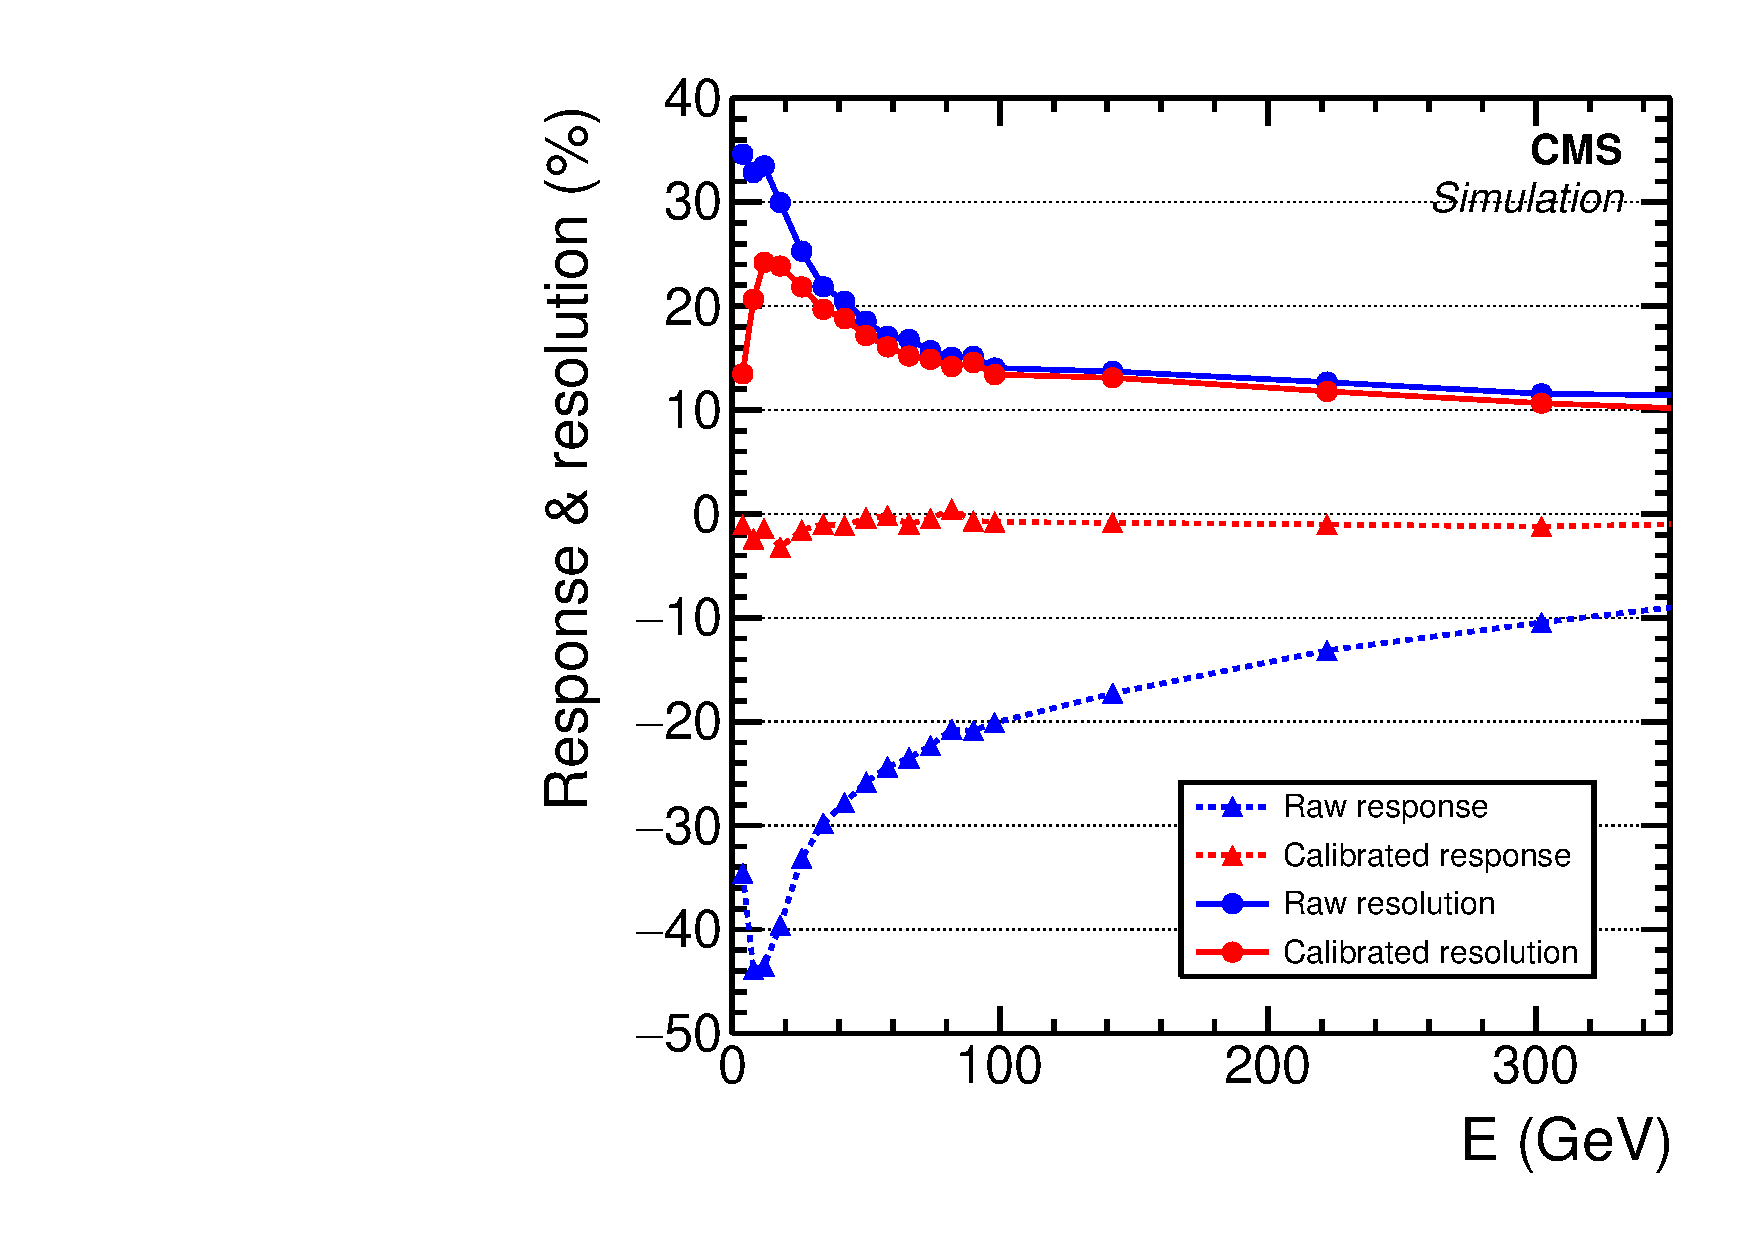
\includegraphics[width=0.45\textwidth]{object_reconstruction_and_selection/plots/calo_response_and_res.pdf}
     \caption{
(left) Calibration coefficients obtained from single $\text{K}^{0}_{\text{L}}$s in the barrel as a 
function of their true energy $E$. The blue triangles show the calibrations for hadrons depositing 
energy only in the HCAL. The red circles (green squares) show the ECAL (HCAL) calibration for hadrons
depositing energy in both the ECAL and HCAL.
(right) Relative raw (blue) and calibrated (red) energy response (dashed curves and triangles) and 
resolution (full curves and circles) for single $\text{K}^{0}_{\text{L}}$s in the barrel, as a 
function of their true energy $E$.
%Here the raw (calibrated) response and resolution are obtained by a Gaussian fit to the distribution of 
%the relative difference between the raw (calibrated) calorimetric energy and the true hadron energy.
     }
     \label{fig:pf_calo_calib}
\end{figure*}


In general, a given particle is expected to result in multiple PF elements (tracks and energy
clusters) in the various CMS subdetectors. The reconstruction of a particle first proceeds 
with a link algorithm that connects the PF elements from different subdetectors. For example,
tracks are linked to energy clusters if the extrapolated position of the track aligns within the
angular acceptance of an energy cluster in \etaphi. Energy clusters can be linked between subdetectors as mentioned
in the case of hadronic energy deposits above which span the ECAL and HCAL. A link is established
when the cluster position in the more granular calorimter, ECAL, is within the cluster envelope
in the less granular calorimeter, HCAL. Once PF elements are linked together they are referred to as a PF block which can contain 
elements associated either by a direct link or by an indirect link through common elements.
The link distance is defined as the distance between the extrapolated track position and the 
cluster position in the \etaphi plane.


\subsection{Particle Flow Candidates}
Particle Flow candidates are selected from the PF blocks based on designated quality cuts.


\subsubsection{Muons}
Isolated global muons are selected from the global muon track colletion by looking at the inner
tracker tracks and calorimeter 
energy deposits within a distance $\dr < 0.3$ to the muon trajectory. 
The sum of the $\pt$ of the tracks and of the ET of the energy deposits is required not to 
exceed 10\% of the muon $\pt$. This isolation criterion alone successfully reject hadrons that would
otherwise be misidentified as muons. No further selection is applied to these muon candidates.
If the muon track $\pt < 200\GeV$, then the momentum assigned to the muon PF candidate is that of 
the inner track. For muon tracks with $\pt > 200\GeV$, the momentum assigned is the momentum associated
with the smallest $\chi^2$ probability from these different track fits: tracker only, tracker and 
first muon detector plane, global, and global without the muon detector planes featuring a high occupancy.
The PF elements and blocks that make up an identified PF muon candidate masked against further processing
to prevent their inclusion in other PF candidates.

In these analyses, there are several additional criteria applied beyond that which is required to
be a PF candidate. These analyses use muons which pass two different PF muon identification working
points: \texttt{PF ID Loose} and \texttt{PF ID Medium}~\cite{sm-htt-2017}. The \texttt{PF ID Loose}
working point is only slightly tighter than the baseline criteria for a PF muon candidate; 
\texttt{PF ID Loose} must be either a global or a tracker PF muon. This selection is highly efficient
for prompt muons.

The \texttt{PF ID Medium} muon working point requires first that muons pass \texttt{PF ID Loose} then
applies additional track-quality and muon-quality requirements on the different muon tracks which are
linked to the PF muon candidate. The number of valide inner tracker
hits must be greater than 80\%. Additionally either one or the other of the following criteria must be met:
\begin{outline}
\1 Option 1 - ``Tight Segment Compatility''
    \2 Candidate has a segment compatility score of at least 0.451 which ensures that the 
track is reasonablly compatible with inner tracker-based track
\1 Option 2 - ``Good Global Muon'':
    \2 PF muon candidate is a global muon
    \2 The normalized track $\chi^2 < 3$
    \2 The compatibility $\chi^2$ between the standalone muon track and the inner tracker muon is
less than 12
    \2 The muon track kink-finder, which is desiged to remove muons produced from in-flight decays, 
must have a value less than 20
    \2 Candidate has a segment compatility score of at least 0.303 which is looser than the value
required in Option 1
\end{outline}
The \texttt{PF ID Medium} muon working is still very efficienct for prompt muon selection but
does bring some additional reduction in fake object selection which is helpful in the high
statistics $htt$ analysis. 

To reject non-prompt or misidentified muons and electrons, a relative lepton isolation is defined as:
\begin{equation}
I^{\ell} \equiv \frac{\sum_{charged}  \pt + \max\left( 0, \sum_{neutral}  \pt
                                         - \frac{1}{2} \sum_{charged, PU} \pt  \right )}{\pt^{\ell}}.
\label{eq:rel_isolation}
\end{equation}

Some of the quantities mentioned here refer to descriptions in the following.
In this expression, $\sum_{charged}  \pt$ is the scalar sum of the transverse energy of the 
charged particles originating from the primary vertex and located in a cone of size
$\dr = \sqrt{\smash[b]{(\Delta \eta)^2 + (\Delta \phi)^2}} = 0.4$\,(0.3)
centered on the muon (electron) direction. The sum, $\sum_{neutral}  \pt$, represents
a similar quantity for neutral particles. The contribution of photons and neutral hadrons 
originating from pileup vertices is estimated from the scalar sum of the transverse
energy of charged hadrons in the cone originating from pileup vertices,
$\sum_{charged, PU} \pt$. This sum is multiplied by a factor of $1/2$, which corresponds 
approximately to the ratio of neutral to charged hadron production in the hadronization process
of inelastic $\Pp\Pp$ collisions, as estimated from simulation. The expression $\pt^{\ell}$ 
stands for the $\pt$ of the lepton. Isolation requirements used in the following analyses, 
based on $I^{\ell}$, range from $I^{\ell} < 0.1$ to $I^{\ell} < 0.25$ depending on the signal efficiency and
background rejection needs of the specific final state. For the $\htt$ analysis, these
working points are listed in the $\htt$ analysis section, table~\ref{tab:htt_obj_selection}.




\subsubsection{Electrons and Prompt Photons}
With the muon related PF elements masked from further processing, electron and prompt photon
identification begins.
Electron identification is based on information from the inner tracker tracks and the calorimeter
energy clusters. Because of bremsstrahlung radiation, electron tracks can be much more kinked
than those for other particles as was discussed above in relation to the GSF algorithm track
fitting. Additionally, because of radiated bremsstrahlung photons, the resulting energy clusters 
from an electron propagating through the detector can be spread out in the
$\phi$ direction. PF electrons are built from the linking of a GSF track to an
ECAL-based energy cluster. To suppress the amount of charged hadrons faking electrons, the 
sum of the energies measured in HCAL hits behind ($\dr < 0.15$) 
the electron-linked ECAL energy cluster must no exceed 10\% of the ECAL-based 
energy cluster energy~\cite{Sirunyan:2017ulk}. The energy assignment for an electron candidate is obtained from a 
combination of the calibrated ECAL energy with the momentum of the GSF track. The electron 
direction is chosen to be that of the GSF track.

Before being saved to the PF electron collection, electron candidates must satisfy additional
identification criteria targeted at reducing electron fakes. Up to fourteen variables are
fed into a Boosted Decision Tree (BDT) which selections the passing PF electrons. The BDT
input variables include track and energy cluster details such as:
\begin{itemize}
\item Amount of energy radiated off the GSF track
\item Distance between the GSF track extrapolation to the ECAL entrance and the position of the ECAL seeding cluster
\item Ratio between the energies gathered in HCAL and ECAL by the track-cluster association process
\item The KF and GSF track $\chi^2$ values, and
\item The numbers of inner tracker hits
\end{itemize}

Photon candidates are seeded by ECAL energy clusters with no matching KF or GSF track.
They are retained as PF photons if they are isolated from other tracks and calorimeter energy clusters, 
and if the ECAL energy distribution and the ratio between the HCAL and ECAL energies, $H/E$, are 
compatible with those expected from a photon shower. Similar to the PF masking after the muon 
reconstruction, tracks and energy clusteres used to
build PF electron and photons are masked from further processing simplifying the task ahead
for charged and neutral hadron identification.

There are additional electron identification requirements used in these analyses which are tighter
than the PF electron criteria. The additional identification criteria relies on a multivariate (MVA) discriminant
which combines many of the same variables used in the PF electron BDT~\cite{Khachatryan:2015hwa} 
and addes some additional energy cluster distribution variables such as: $\sigma_{i\eta i\eta}$ and
$\sigma_{i\phi i\phi}$ cluster shape covariance. The analyses use
two different MVA working points, one with 90\% signal efficiency and one with 80\% efficiency.


\subsubsection{Charged and Neutral Hadrons}
Once muons, electrons, and isolated photons are identified and removed from the available PF blocks
and elements, the remaining particles to be identified are hadrons resulting from jet fragmentation and 
hadronization. The ECAL and HCAL energy clusters which are not linked to any tracks are turned into
PF neutral hadrons while energy deposits successfully linked to a track are turned into PF charged
hadrons. Non-isolated photons are indistinguishable from the neutral hadron group and are considered
as part of that collection. Charged and neutral hadron form the last sets of fundamental physics-objects
which are reconstructed by PF. The next PF steps involve reconstructing composit object such as ``jets''
and hadronically decaying tau leptons and calculating event quantities such as the primary vertex and
\etvecmiss.


\section{Event Level Quantities}
There are multiple event level quantities that require input from all PF physics-objects for their
calculation. The calculation of the primary vertex is specifically needed for the identification of
composit objects such as ``jets'' and hadronically decaying $\tau$ leptons.


\subsection{Primary Vertex Reconstruction}
The original location of the $\pp$ collisions which gave rise to a given event can be found by tracing
the reconstructed physics-object tracks back to the collision region and grouping together tracks that share a common
origin; the origins are called vertices. In any given recorded collision there will be usually be a 
singular hard-scatter $\pp$ collision and multiple soft-scatter collsion. The hard-scatter vertex is 
identified as the vertex with the largest quadratic sum of the $\pt$ of the associated physics-objects 
and is called the primary vertex~\cite{Sirunyan:2017ulk}. The other vertices are referred to as the
pileup vertices.


\subsection{Missing Transverse Energy}
The CMS detector can detect and measure the energy of all standard model particles with the exception
of neutrinos which leave the detector undetected. The neutrino energy contribution to an event can
be estimated using the missing transverse energy, \etvecmiss. The \etvecmiss is calculated from
the raw missing transverse momentum vector which is defined 
to balance the vectorial sum of the transverse momentum of all particles.

\begin{equation}
\vec{p}^{\text{miss}}_{\text{T,PF}}(\text{raw}) = - \sum^{N_{\text{particles}}}_{i=1} \vec{p}_{\text{T},i}
\end{equation}

All particles reconstructed in the event are used to determine the missing transverse energy,
\etvecmiss~\cite{Khachatryan:2014gga}. The specific \etvecmiss used in these analyses is Type-1
\etvecmiss which is adjusted for the effect of jet energy corrections.


\section{Composit Object Identification and Selection}
Composit objects reconstructed by PF attempt to cluster together physics-objects which likely
resulted from the jet fragmentation or hadronization process. The three groups used in these
analyses are discussed below.

 
\subsection{Jets}
Jets are collections of energy deposits and tracks within a defined conical area radiating outward
from the collision region. They are created when a quark or gluon undergoes the hadronization process.
Jets are reconstructed with an anti-\kt clustering algorithm implemented in the \FASTJET 
library~\cite{Cacciari:2008gp, Cacciari:2011ma, Cacciari:fastjet2}. The anti-\kt clustering is based on the grouping
together of neutral and charged PF candidates within a distance parameter $\dr = 0.4$. Charged PF 
candidates not associated with the primary vertex are not considered when building jets.
A correction is applied to jet energies to adjust for the contribution to the jet energy from 
additional $\pp$ interactions within the same or nearby bunch crossings. The energy of a jet is 
corrected via calibrations based on simulation and data~\cite{CMS-JME-10-011}.


\subsection{Taus}
Hadronically decaying $\Pgt$ leptons
are reconstructed with the hadron-plus-strips (HPS)
algorithm~\cite{Khachatryan:2015dfa, CMS-PAS-TAU-16-002}, which is
seeded with anti-\kt jets.
The HPS algorithm reconstructs $\tauh$ candidates on the basis of the
number of tracks and of the number of ECAL strips in the $\eta$-$\phi$ plane with energy deposits, in the 1-prong,
1-prong + $\PGpz$(s), and 3-prong decay modes. A
multivariate (MVA) discriminator~\cite{Hocker:2007ht}, including isolation
and lifetime information, is used to reduce the rate for  quark- and gluon-initiated jets
to be identified as $\tauh$ candidates. The working point used in this analysis
has an efficiency of about 60\% for genuine $\tauh$,
with about 1\% misidentification rate for quark- and gluon-initiated jets, for a $\pt$ range typical of $\tauh$ originating from a $\PZ$ boson.
Electrons and muons misidentified as $\tauh$ candidates are suppressed using dedicated criteria
based on the consistency between the measurements in the tracker, the calorimeters, and the muon detectors~\cite{Khachatryan:2015dfa, CMS-PAS-TAU-16-002}.
The working points of these discriminators depend on the
decay channel studied.


\subsection{b-jet ID and Secondary Vertex}
The combined secondary vertex (CSV) algorithm is used to identify jets that are likely to originate from a b quark (``b jets"). The algorithm exploits the track-based lifetime information together with the secondary vertices associated with the jet to provide a likelihood ratio discriminator for the b jet identification. A set of $\pt$-dependent correction
factors are applied to simulated events to account for differences in the b tagging efficiency
between data and simulation. The working point chosen in this analysis gives an efficiency for real b jets of about 70\%, and for about 1\% of light flavor or quark jets being misidentified.



\chapter{Higgs $\to \tau\tau$: Gluon Fusion and Vector Boson Fusion}
\label{sec:htt_analysis}

This chapter describes a study of Higgs boson production and subsequent
decay to a pair of $\tau$ leptons using CMS proton-proton collision data gathered in 2016. 
This chapter specifically discusses a study targeting the gluon fusion ($ggH$) and
vector boson fusion (VBF) Higgs boson production mechanisms. A later chapter, ~\ref{sec:vh_analysis},
discusses a study focusing on the associated production Higgs boson mechanism.
This gluon fusion and VBF targeted study is the first
$\htt$ analysis performed using center-of-mass energy 13 TeV data from the LHC. Combining
these 13 TeV results with 7 TeV and 8 TeV CMS $\htt$ results we produce
the first single experiment observation of the $\htt$ process, observed at the 5.9 $\sigma$
confidence level. Additionally, this study provides the strongest constraints on VBF Higgs 
production to date for all CMS Higgs boson analyses.



\section{Overview}

This chapter specifically focuses on studying the Higgs boson produced via the gluon fusion
or the VBF production mechanisms. A study of the Higgs boson produced in associated production with
$\PW\PH$/$\PZ\PH$ is presented in Chapter~\ref{sec:vh_analysis}. This study utilizes the
full 2016 $\pp$ dataset collected by CMS corresponding to 35.9$\fbinv$ of integrated luminosity.
In the following pages the symbol $\ell$ refers to electrons and muons and $\tauh$ refers to hadronically
decaying $\tau$ leptons. We study all possible $\tau\tau$ final state combinations with the
exception of two electron and two muon final states because of the low 
$\tau\tau \to \tau_{e}\tau_{e}/\tau_{\mu}\tau_{\mu}$
branching fractions and high background from $\PZ \to ee/\mu\mu$. The $\htt$ final states which are
studied are: $\tau_{e}\tauh$ denoted here as $\Pe\tauh$, $\tau_{\mu}\tauh$ denoted as $\Pgm\tauh$,
$\tau_{e}\tau_{\mu}$ denoted here as $\Pe\Pgm$, and lastly, $\tauh\tauh$ denoted as $\tauh\tauh$.
This combination of final states covers about 94\% of all possible $\tau\tau$ final states.
The different $\tau\tau$ final states will be refered to as different channels in the following pages.
We ensure uniqueness between the four studied channels be applying veto criteria to events based
on the number of reconstructed loosely identified electrons and muons. This ensures that 
no data or simulated event is double counted in two channels.

Selected events are classified into three different categories targeting different characteristics
of the gluon fusion and VBF production topologies. The categories are defined according to the
number and kinematics of the associated jets in each event along with the reconstructed $\pt^{Higgs}$.
A number of different control regions are used in the final fit for signal extraction. This allows
the fit to simultaneously adjust and constrain all processes targeted by a control region. This is in
contrast to extracting a scale factor which is applied as a fixed value in an analysis which is not
allowed to adjust as other background process adjust in the final fit. The backgrounds which are
targeted with dedicated control regions are: $\PW$+jets, QCD multijet, and $\ttbar$.



\subsection{Event Selection}

There are specific baseline criteria applied to all electrons, muons, $\tauh$, and jets for every
event. Depending on the final state, additional requirements are placed on these objects based
on suppressing target backgrounds or to meet trigger requirements and analysis optimization. The baseline criteria ensure
that each object is well reconstructed and well identified and consistent with the analysis
strategy. 

\subsection{Triggers}
\label{sec:htt_triggers}
Selected events are required to to have fired a high level trigger consisten with their categorized final
state channel. For the $\Pgm\tauh$ channel, events are selected using a combination
of a single isolationed muon trigger as well as a cross trigger firing on an isolated muon and
an isolated $\tauh$. The $\Pgm\tauh$ cross trigger allows for a lower $\pt$ threshold
on the selected muon. In contrast, due to the HLT menu available in 2016, the $\Pe\tauh$ cross triggers
do not bring a substantial increase in acceptance and were not used in this analysis.
For the $\Pe\tauh$ channel, events are selected using only a trigger firing on a 
single isolated electron. For the $\Pe\Pgm$ channel, events are selected with electron-muon cross
triggers requiring an isolated online electron and an isolated online muon. There are two 
different electron-muon corss triggers used with their HLT $\pt$ thresholds detailed following.
For the $\tauh\tauh$ channel, events are selected using an online criteria of two loosely isolated $\tauh$. 
The HLT paths used and their online $\pt$ thresholds are detailed in table~\ref{tab:htt_hlt_triggers}.

Due to changing data gathering conditions and a changing HLT menu throughout 2016 data taking, the HLT path
requirements changed throughout 2016 and are era dependant. During latter eras, at higher instantaneous 
luminsity, some HLT paths became diabled or prescaled. The study avoids using any prescaled
HLT paths. For the $\Pgm\tauh$ channel this 
leads to changes in the $\abs\eta$ requirement on the online muon in the single muon triggers.
There are two muon-tau cross triggers available throughout 2016. One of them requires only the
presence of a single muon at the Level-1 trigger and has ``SingleL1'' appended to its path
name. The other requires the presence of both a muon and a $\tauh$ at the Level-1 trigger.
The single electron trigger used in the $\Pe\tauh$ channel remained constant through the year.
Due to changing pileup conditions and increasing luminosity during the final eras, the online
isolation criteria was changed for the $\tauh\tauh$ channel triggers. The online $\tauh$ 
isolation changed from being based on purely charged energy deposits to being based on a 
combination of charged and neutral based energy deposits. The triggers used in the
$\Pe\Pgm$ channel changed during the final two eras, G and H, and had a lepton DZ filter
applied to them. The DZ filter requires that the electron and muon match to the HLT primary
vertex. This is a common method used to reduce rate at the HLT. In all channels, the electrons, muons, and
$\tauh$ in each event must be matched to within $\Delta R < 0.5$ with the associated
HLT object which triggered the event.


\begin{table*}[htbp]
\centering
\begin{footnotesize}
%\begin{scriptsize}
\begin{tabular}{|l|l|l|l|}
\hline
  Channel           &         Trigger $\pt$ Req.              &     High Level Trigger Path  &   Eras  \\
\hline
  $\mu\tauh$       &         $\Pgm(22)$                     &  \scriptsize{HLT\_IsoMu22\_v*} & B-F  \\ 
                   &         $\Pgm(22)$                     &  \scriptsize{HLT\_IsoTrkMu22\_v*} & B-F   \\ 
                   &         $\Pgm(22)$                     &  \scriptsize{HLT\_IsoMu22\_eta2p1\_v*} & C-H  \\
                   &         $\Pgm(22)$                     &  \scriptsize{HLT\_IsoTrkMu22\_eta2p1\_v*} & C-H   \\
                   &         $\Pgm(19)\,\&\,\tauh (20)$     &  \scriptsize{HLT\_IsoMu19\_eta2p1\_LooseIsoPFTau20\_SingleL1\_v*} &  All Eras  \\
                   &         $\Pgm(19)\,\&\,\tauh (20)$     &  \scriptsize{HLT\_IsoMu19\_eta2p1\_LooseIsoPFTau20\_v*} &  All Eras \\
\hline
  $\Pe\tauh$       &         $\Pe (25)$                     &  \scriptsize{HLT\_Ele25\_eta2p1\_WPTight\_Gsf\_v*}   & All Eras \\
\hline
 $\tauh\tauh$      &         $\tauh (35)\,\&\,\tauh (35)$   &  \scriptsize{HLT\_DoubleMediumIsoPFTau35\_Trk1\_eta2p1\_Reg\_v*} & B-G   \\ 
                   &         $\tauh (35)\,\&\,\tauh (35)$   &  \scriptsize{HLT\_DoubleMediumCombinedIsoPFTau35\_Trk1\_eta2p1\_Reg\_v*} & H  \\
\hline
  $\Pe\Pgm$        &         $\Pe(12)\,\&\,\Pgm (23)$       &  \scriptsize{HLT\_Mu23\_TrkIsoVVL\_Ele12\_CaloIdL\_TrackIdL\_IsoVL\_v*} & B-F \\
                   &         $\Pe(12)\,\&\,\Pgm (23)$       &  \scriptsize{HLT\_Mu23\_TrkIsoVVL\_Ele12\_CaloIdL\_TrackIdL\_IsoVL\_DZ\_v*} & G-H  \\
                   &         $\Pe(23)\,\&\,\Pgm (8)$        &  \scriptsize{HLT\_Mu8\_TrkIsoVVL\_Ele23\_CaloIdL\_TrackIdL\_IsoVL\_v*} & B-F  \\
                   &         $\Pe(23)\,\&\,\Pgm (8)$        &  \scriptsize{HLT\_Mu8\_TrkIsoVVL\_Ele23\_CaloIdL\_TrackIdL\_IsoVL\_DZ\_v*} & G-H  \\
\hline
\end{tabular}
\end{footnotesize}
%\end{scriptsize}
\caption{For each channel the online HLT $\pt$ threshold is listed along with the specific associated
HLT paths. Throughout 2016 data taking, the HLT menu changed to respond to changing online
conditions at CMS and the LHC. This is reflected in progressively tighter triggers
being available towards the end of the 2016 run.
\label{tab:htt_hlt_triggers}
}
\end{table*}



\subsection{Baseline Object Selection}
\label{sec:htt_obj_sel}
All electrons and muons must meet the minimum requirement
that the distance of closest approach to the primary vertex satisfies $\abs{d_z}<0.2$ cm
along the beam direction, and $\abs{d_{xy}}<0.045$ cm in the transverse plane. Ensuring
compatibility with the primary vertex is consistent with the predicted infinitesimal life-time of
a Higgs boson. The HPS reconstruction of $\tauh$ detailed in section~\ref{sec:XXX} can involve
combining together multiple tracks and $\PGpz$s coming from intermediary $\tau$ decay products.
Due to these intermediary products, the reconstructed $d_{xy}$ for $\tauh$ are often
larger than those for electrons and muons. Because of this, the primary vertex matching
criteria are relaxed for $\tauh$ and only require $\abs{d_z}<0.2$ cm.

The offline selection criteria for all electrons, muons, and $\tauh$ are motivated and constrained
by the High Level Trigger requirements of their path. Specifically, the offline $\pt$ criteria
applied are always higher than the HLT $\pt$ threshold to ensure a stable measurement and application
of trigger efficiencies. An offline $\pt$ threshold applied right at the HLT $\pt$ threshold
makes measurement of the steeply rising efficiency at the HLT threshold absolutly critical.
This is very difficult to do perfectly and would lead to very large trigger systematics
at low $\pt$ in the turn-on region. Additionally, there are offline $\eta$ restrictions
enforced which align with those at the HLT.

All selected electrons, muons, and $\tauh$ must be well identified and isolated from overlapping
energy deposits and reconstructed objects. This study uses identification criteria
provided centrally by the CMS Physics Object Groups (POGs). All identification and isolation
working points used have been selected through an optimization process selecting
for increased analysis sensitivity. The optimimum working points strike a balance
between signal efficiency and background rejection. For electrons an MVA-based ID
is used in both the $\Pe\tauh$ and $\Pe\Pgm$ channels which has been tuned to provide 
80\% electron selection efficiency. Muons in both the $\mu\tauh$ and $\Pe\Pgm$ channels
require the Particle Flow Medium ID. The selection of $\tauh$ relies on MVA-based working
points. The $\tauh$ MVA-based working points combine both object identification and object
isolation together into a single set of working points. Table~\ref{tab:htt_obj_selection}
details the $\pt$, $\abs\eta$, identification and isolation criteria for all electrons, muons,
and $\tauh$ selected in the study.


\begin{table*}[htbp]
\centering
\begin{small}
\begin{tabular}{l|l|l|l|l}
  Channel       & $\pt$ ($\GeV$) & $\eta$ & Identification & Isolation \\
\hline
  $\mu\tauh$       &   $\pt^\Pgm>20$     &  $\abs{\eta^\Pgm}<2.1$    &   PF ID Medium &  $I^{\Pgm}<0.15$       \\
                   &   $\pt^{\tauh}>30$  &  $\abs{\eta^{\tauh}}<2.3$ &   MVA $\tauh$ ID Tight & MVA $\tauh$ ID Tight \\
\hline
 $\tauh\tauh$      &   Leading $\pt^{\tauh}>50$ & $\abs{\eta^{\tauh}}<2.1$  &    MVA $\tauh$ ID Tight    & MVA $\tauh$ ID Tight    \\
                   &   Subleading $\pt^{\tauh}>40$ & $\abs{\eta^{\tauh}}<2.1$  &    MVA $\tauh$ ID Tight & MVA $\tauh$ ID Tight    \\
\hline
  $\Pe\tauh$       &   $\pt^\Pe>26$      & $\abs{\eta^\Pe}<2.1$       &   MVA 80\% WP  &  $I^{\Pe}<0.1$  \\
                   &   $\pt^{\tauh}>30$  &  $\abs{\eta^{\tauh}}<2.3$  &   MVA $\tauh$ ID Tight & MVA $\tauh$ ID Tight \\
\hline
  $\Pe\Pgm$        &   $\pt^{\Pe}>13$    & $\abs{\eta^\Pe}<2.5$   &   MVA 80\% WP   & $I^{\Pe}<0.15$   \\
                   &   $\pt^{\Pgm}>15$   & $\abs{\eta^\Pgm}<2.4$  & PF ID Medium &  $I^{\Pgm}<0.2$    \\
\hline
\end{tabular}
\end{small}
\caption{Kinematic, identification and isolation selection requirements for the four di-$\Pgt$ channels.
\label{tab:htt_obj_selection}
}
\end{table*}


The three different signal extraction categories rely on the details of reconstructed jets, or
lack there of, in each event.  Jets are reconstructed using the anti-$k_{\text{T}}$ algorithm with distance
parameter $\Delta\text{R}=0.4$~\cite{Cacciari:2008gp}.  Charged hardons that are not consistent with
the primary vertex are removed from the anti-$k_{\text{T}}$ clustering.  Jets are only considered
if they pass they pass the loose working point of the PF Jet ID discriminator~\cite{jetID}.
Jets must have $\pt > 30 \GeV$ and $\abs\eta<4.7$.  The $\pt$ and $\eta$ requirements are altered
for cases where the jet is identified as having likely originated from a b-quark.  Jets likey originating
from a b-quark are considered if they pass the CSVv2 Medium working point are then labeled as b-tagged jets.
B-tagged jets have a relaxed $\pt$ requirement but much tighter $\eta$ requirement: $\pt > 20 \GeV$ 
and $\abs\eta<2.4$.  The tightened $\eta$ requirment necessitates that b-tagged jets are located within
the detector volumne fully covered by the CMS pixel and strip tracker.
Lastly, all jets must be separated from the selected electrons, muons, and $\tauh$ by $\Delta\text{R}>0.5$.

Depending on the di-$\tauh$ channel, there are specific topological cuts targeted at significantly
reducing the contribution of certain background processes in the signal region.  The large $\PW+\text{jets}$
cross section combined with a non-negligible jet $\to \tauh$ fake rate leads to a large $\PW+\text{jets}$
contribution in the $\ell\tauh$ channels.  This contribution is significantly reduced at the cost of
minimal signal events by cutting on the transverse mass, $\MT$.  Where the $\MT$ selection is defined as,

\begin{equation}
\MT \equiv \sqrt{\smash[b]{2 \pt^\ell \ptmiss [1-\cos(\Delta\phi)]}} < 50\GeV,
\end{equation}

where $\pt^\ell$ is the transverse momentum of the lepton $\ell$,
and $\Delta\phi$ is the azimuthal angle between its direction and the \etvecmiss.

In the $\Pe\Pgm$ channel, the large \ttbar background is reduced by requiring 
$p_\zeta - 0.85 \, p_\zeta^{\text{vis}} > -35$ or $-10$\GeV depending on which category the event is
classified within.  $p_\zeta$ is the component of the \etvecmiss projected along the bisector 
of the transverse momenta of the two leptons and $p_\zeta^{\text{vis}}$ is the sum of the components 
of the lepton transverse momenta along the same direction~\cite{Khachatryan:2014wca}, also see
figure~\ref{fig:htt_pZeta} for visual reference.
The $p_\zeta$ selection criteria has a high signal efficiency. The \etvecmiss is typically oriented
in the same direction as the visible di-$\Pgt$ system in signal events because the \etvecmiss is 
the results of neutrinos from the signal $\tau$s.  The orientation of the \etvecmiss with respect
to the di-$\tau$ system is much less predictable in \ttbar events.  In addition, events with a b-tagged 
jet are discarded to further suppress the \ttbar background in the $\Pe\Pgm$ channel.

\begin{figure*}[htbp]
\centering
     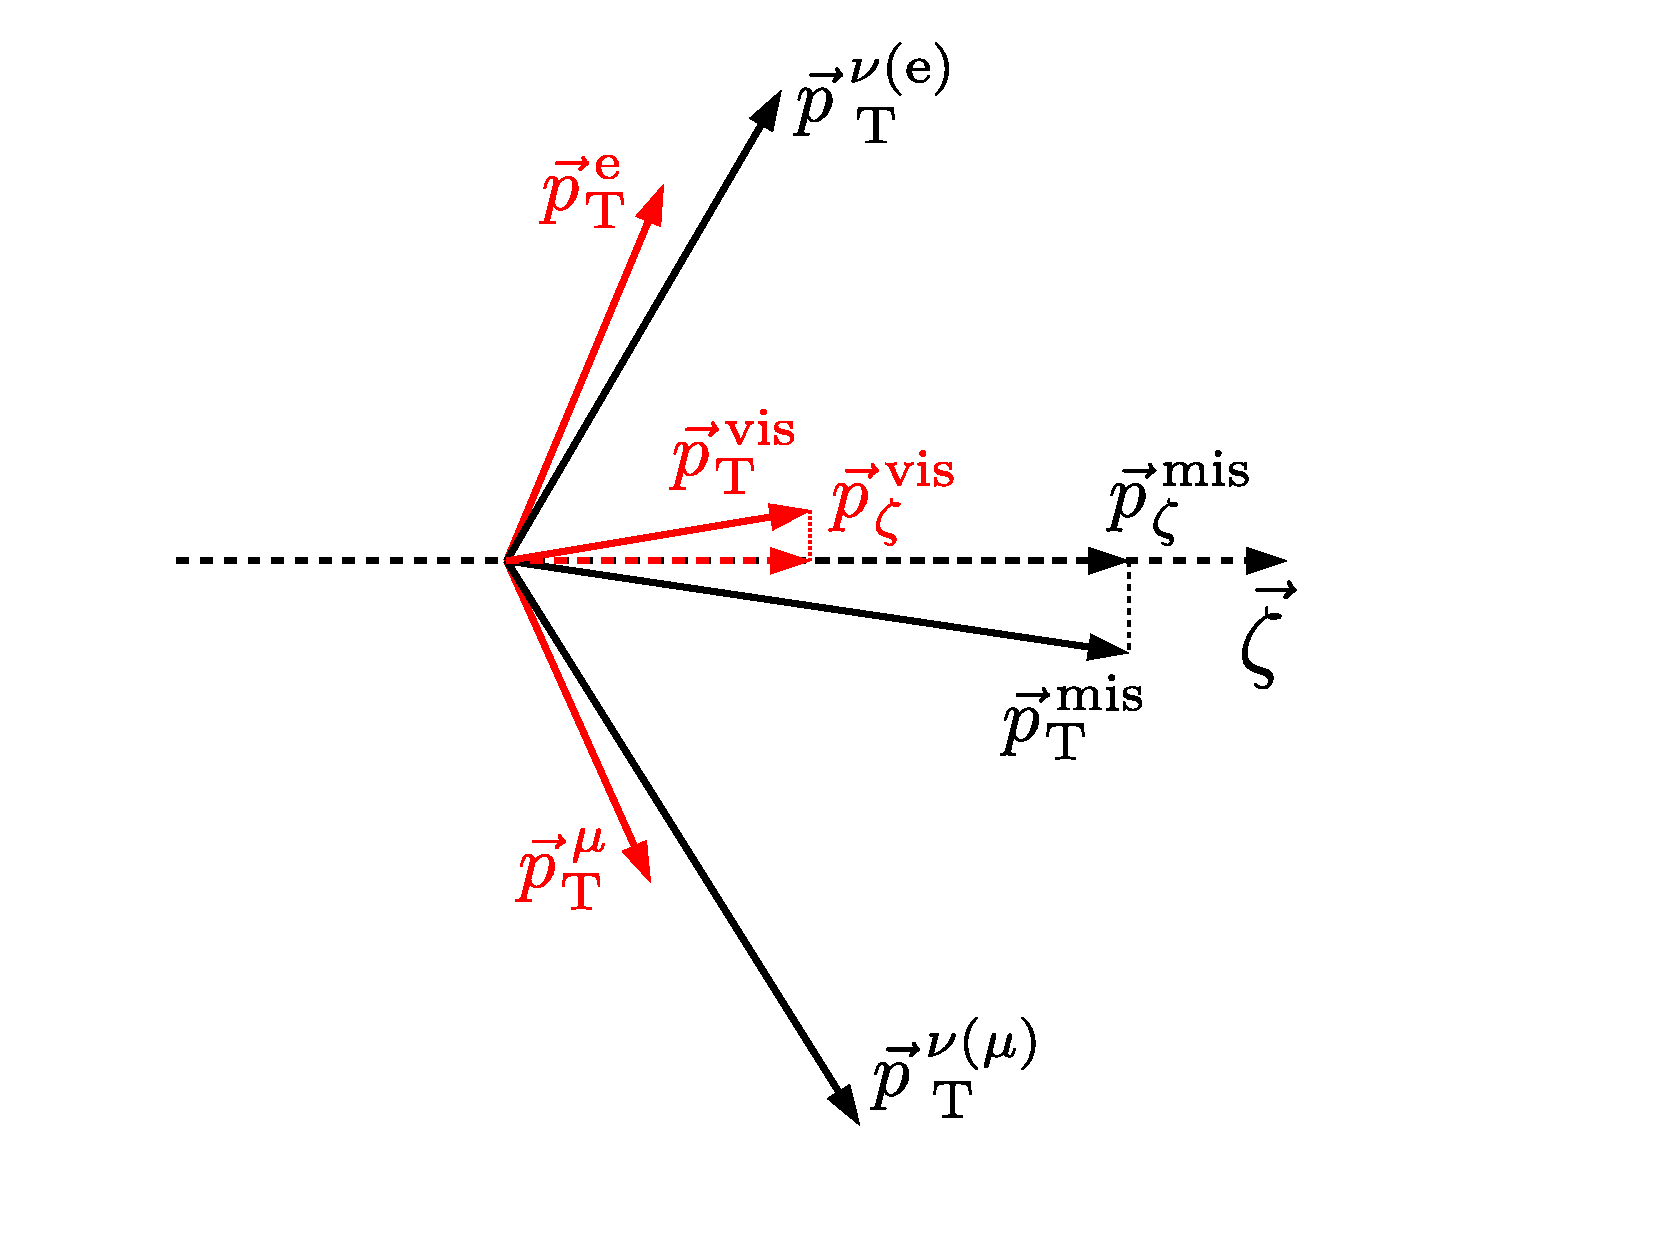
\includegraphics[width=0.4\textwidth]{higgs_to_taus/plots/pZeta_def.pdf}
     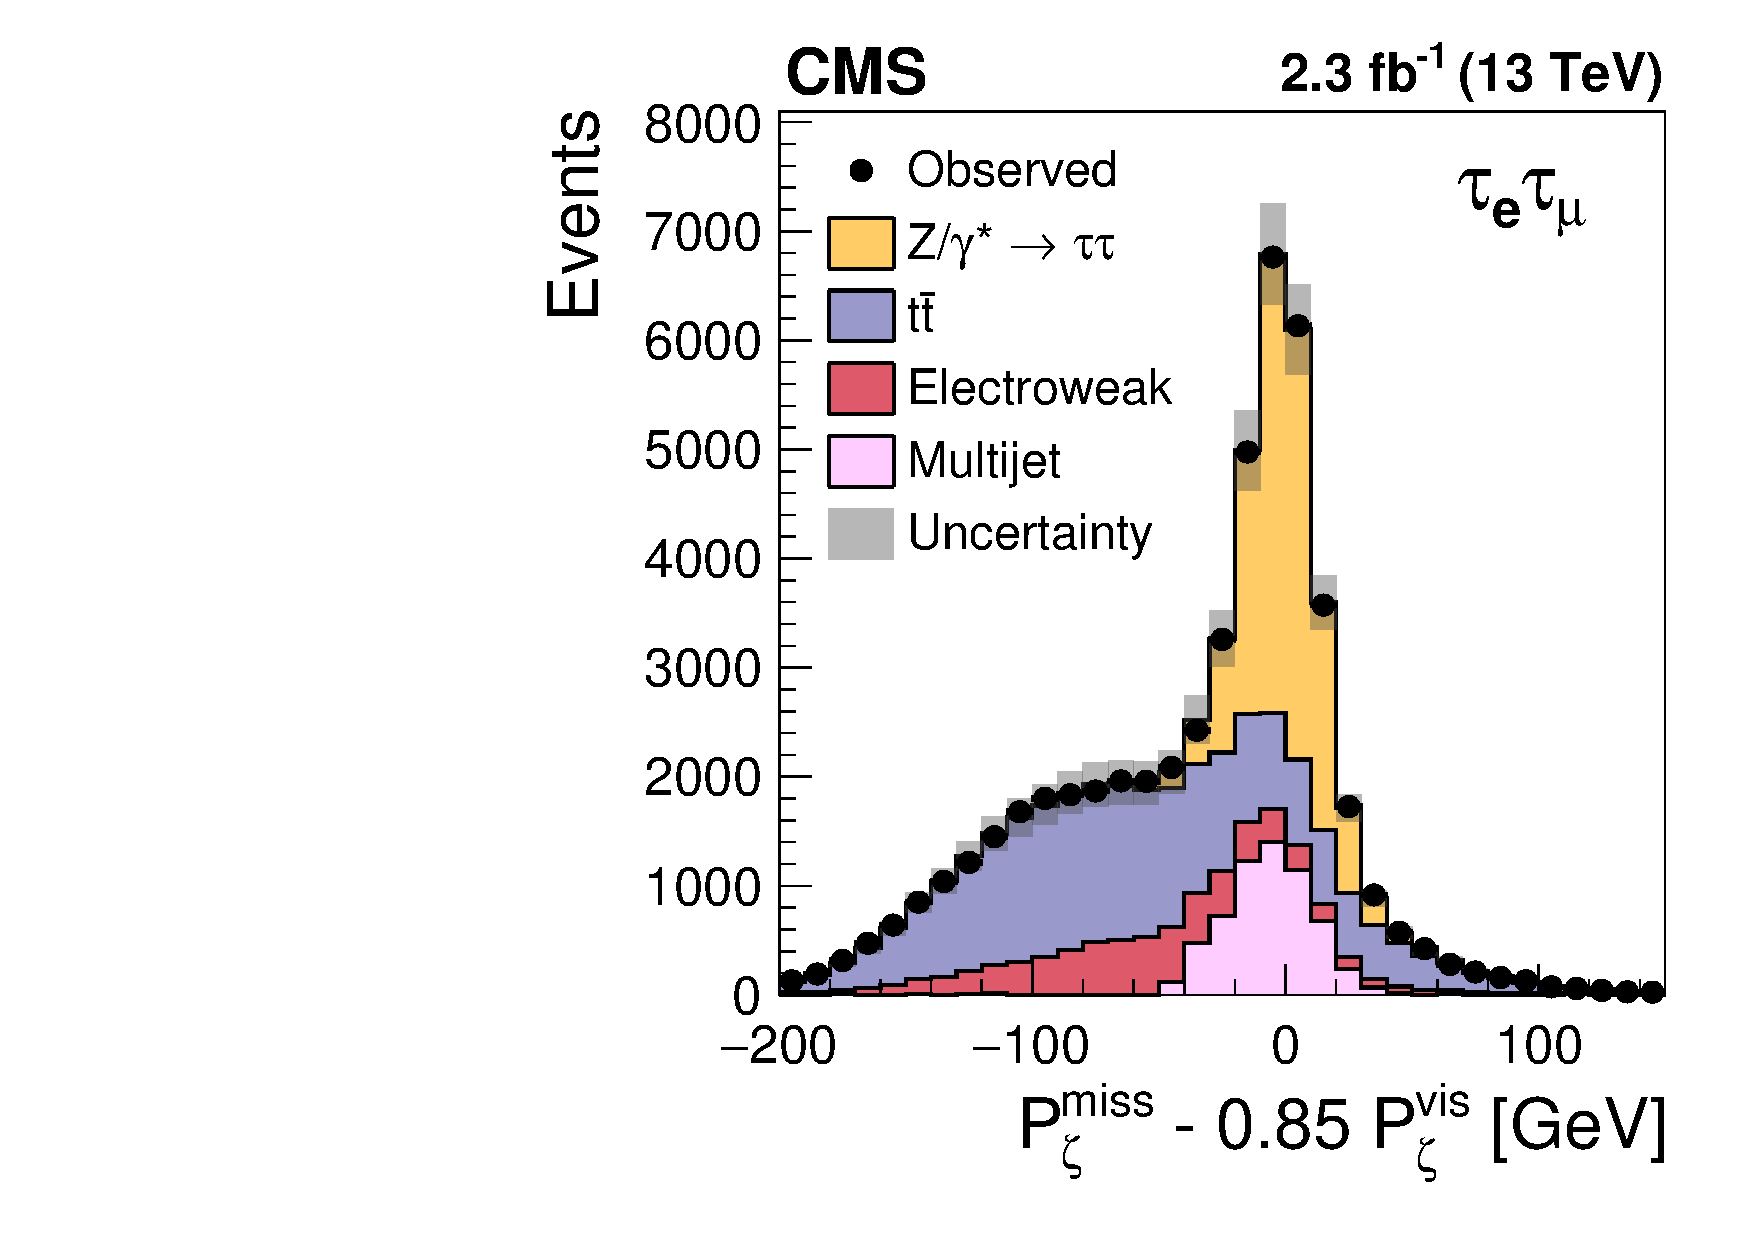
\includegraphics[width=0.4\textwidth]{higgs_to_taus/plots/htt_em_pZeta.pdf}\\
     \caption{
(Left) Diagram showing the construction of the $p_\zeta$ and $p_\zeta^{\text{vis}}$ projections.
(Right) An example $p_\zeta - 0.85 \, p_\zeta^{\text{vis}}$ distribution is shown for a similar but not
overlapping selection in the $\Pe\Pgm$ channel.  This distribution is from an analysis focusing on specifically studying the
$\PZ\to\tau\tau$ process~\ref{HIG-15-007}.
In the $\htt$ analysis, the Higgs boson $p_\zeta - 0.85 \, p_\zeta^{\text{vis}}$
spectrum aligns very closely with the $Z\to\tau\tau$ distribution shown here.
     }
     \label{fig:htt_pZeta}
\end{figure*}

\subsection{Categorization}

Selected events are split into three mutually exclusive categories per decay channel.
The categories are designed to target different aspects of the gluon fusion and VBF Higgs boson production mechanisms.
In each category the two variables that maximize the $\PH\to\Pgt\Pgt$ sensitivity are chosen to build 
two-dimensional (2D) distributions.

The three categories are defined as:
\begin{itemize}
\item {0-jet}: This category targets Higgs boson events produced via gluon fusion.
The two variables chosen to extract the results are $\mvis$ and
the reconstructed $\tauh$ decay mode in the $\Pgm\tauh$ and $\Pe\tauh$ decay channels.
In the $\Pe\Pgm$ channel, $\mvis$ and the $\pt$ of the muon are used. The $\PZ\to\ell\ell$ background 
is large in the 1-prong and 1-prong + $\PGpz$(s) $\tauh$ decay modes in the
$\Pgm\tauh$ and $\Pe\tauh$ channels. By using only $\mvis$ instead of $\mtt$ the \etvecmiss
does not smear the mass reconstruction for $\PZ\to\ell\ell$ which retains a nice sharp peak.
The sharp Z peak of $\PZ\to\ell\ell$ provides 
an excellent handel to distinguish $\PZ\to\ell\ell$ from the other background process and
helps constrain the associated uncertainties for electrons and muons faking $\tauh$.
As electrons and muons almost exclusively fake 1-prong and 1-prong + $\PGpz$(s) $\tauh$,
the reconstructed $\tauh$ decay mode is used as the second of the 2D variables in the
$\Pgm\tauh$ and $\Pe\tauh$ channels. Additionally, the lack of $\PZ\to\ell\ell$ in the
3-prong decay mode results in increased signal significance for that region.
Examples of the 2D distributions for the signal and $\PZ\to\ell\ell$ background
in the 0-jet category of the $\Pgm\tauh$ decay channel are shown in Fig.~\ref{fig:htt_2Dcategories} (top).
In the $\tauh\tauh$ decay channel, only one observable, $\mtt$, is considered because of the low
event yields due to the relatively high $\pt$ thresholds on the $\tauh$ at trigger level, and 
because of the sharply falling $\tauh$ $\pt$ distribution. Simulations indicate that about 98\% 
of signal events in the 0-jet category correspond to Higgs bosons produced via the gluon 
fusion production mechanism.

\item {VBF}: This category targets Higgs boson events produced via the VBF process.
The presence of jets from the hard scattering process in VBF production leads the study to heavily
utilize jet kinematics and the jet topology in the VBF category.
Events are selected with at least two (exactly two) jets with $\pt>30$\GeV in the
$\tauh\tauh$, $\Pgm\tauh$, and $\Pe\tauh$ ($\Pe\Pgm$) channels.
In the $\Pgm\tauh$, $\Pe\tauh$, and $\Pe\Pgm$ channels, the two leading jets are required to have 
an invariant mass, $\mjj$, larger than 300\GeV. The variable $\pth$, defined as the magnitude 
of the vectorial sum of the $\ptvec$ of the visible decay products of the $\Pgt$ leptons 
and $\etvecmiss$, is required to be greater than 50 (100)\GeV in the $\Pgm\tauh$
 and $\Pe\tauh$ ($\tauh\tauh$) channels to reduce the contribution from $\PW+\text{jets}$ 
backgrounds. This selection criterion also suppresses the background from quantum 
chromodynamics (QCD) multijet events. In addition, the $\pt$ threshold on the $\tauh$ 
candidate is raised to 40\GeV in the $\Pgm\tauh$ channel. The two leading jets in the 
$\tauh\tauh$ channel should be separated in pseudorapidity by $\Delta\eta>2.5$. The $\Delta\eta>2.5$
cut in the $\tauh\tauh$ channel significantly reduces the contributions from QCD multijet events at the cost
of very few signal events because of the large jet $\Delta\eta$ in genuine VBF events.
The two observables used in the VBF category are $\mtt$ and $\mjj$ for all channels. Example 2D 
distributions for the signal and $\PZ\to\Pgt\Pgt$ background
in the VBF category of the $\Pgm\tauh$ decay channel are shown in Fig.~\ref{fig:htt_2Dcategories} (center). 
Integrating over the whole $\mjj$ phase space, up to 57\% of the signal events in the VBF 
category are produced in the VBF production mode, but this proportion increases with $\mjj$ allowing
for signal production process discrimination in the highest $\mjj$ ranges.

\item {Boosted}: This category contains all selected events that do not enter one of the previous 
categories, namely events with one jet and events with several jets that fail the specific requirements of the VBF category.
The Boosted category contains a mix of gluon fusion events produced in association with one or more jets (78--80\% of signal events),
VBF events where one of the jets escaped detection or has low $\mjj$ (11--13\%), as well as
Higgs bosons produced in association with a $\PW$ or a $\PZ$ boson decaying hadronically (4--8\%).
Because these gluon fusion events failed the 0-jet category, the Higgs boson will be recoiling 
off of one or more jets making the $\pth$ a natural choice for the second distribution variable with
$\mtt$ as the other of the 2D variables. 
Most background processes, including $\PW+\text{jets}$ and QCD multijet events, typically have low $\pth$. 
Example 2D distributions for the signal and $\PW+\text{jets}$ background in the Boosted category of 
the $\Pgm\tauh$ decay channel are shown in Fig.~\ref{fig:htt_2Dcategories} (bottom).
\end{itemize}

In figure~\ref{fig:htt_2Dcategories}, the background processes are chosen for illustrative 
purpose for their separation from 
the signal. The $\PZ\to\Pgm\Pgm$ background in the 0-jet category is concentrated in 
the regions where the visible mass is close to 90\GeV and is negligible when the $\tauh$ 
candidate is reconstructed in the 3-prong decay mode. The $\PZ\to\Pgt\Pgt$ background in 
the VBF category mostly lies at low $\mjj$ values whereas the distribution of VBF signal 
events extends to high $\mjj$ values. In the Boosted category, the W+jets background, 
which behaves similarly to the QCD multijet background, is rather flat with respect to $\mtt$, and 
is concentrated at low $\pth$ values.

The three categories and the variables used to build the 2D distributions are summarized in
Table~\ref{tab:htt_categories}. 

\begin{figure*}[htbp]
\label{fig:htt_2Dcategories}
\centering
     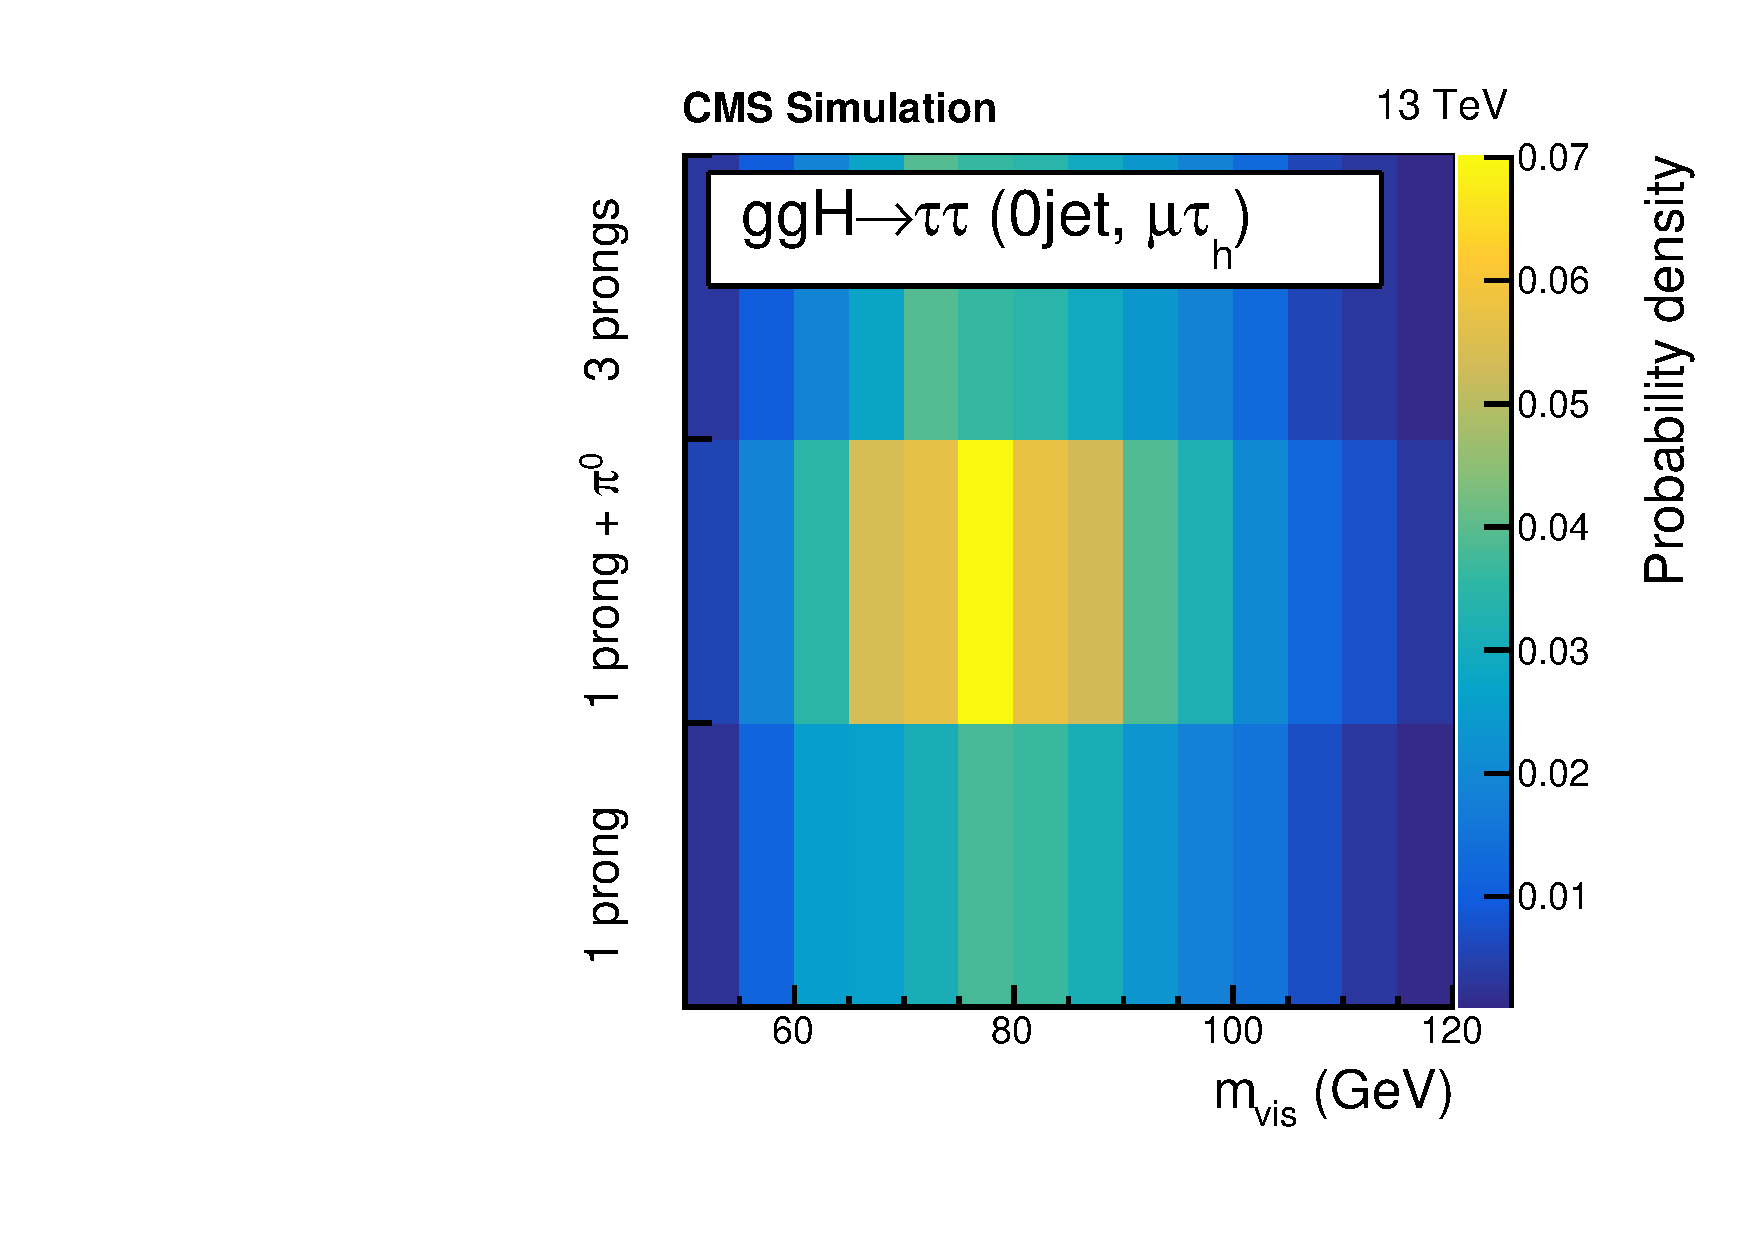
\includegraphics[width=0.4\textwidth]{higgs_to_taus/plots/Figure_001-a.pdf}
     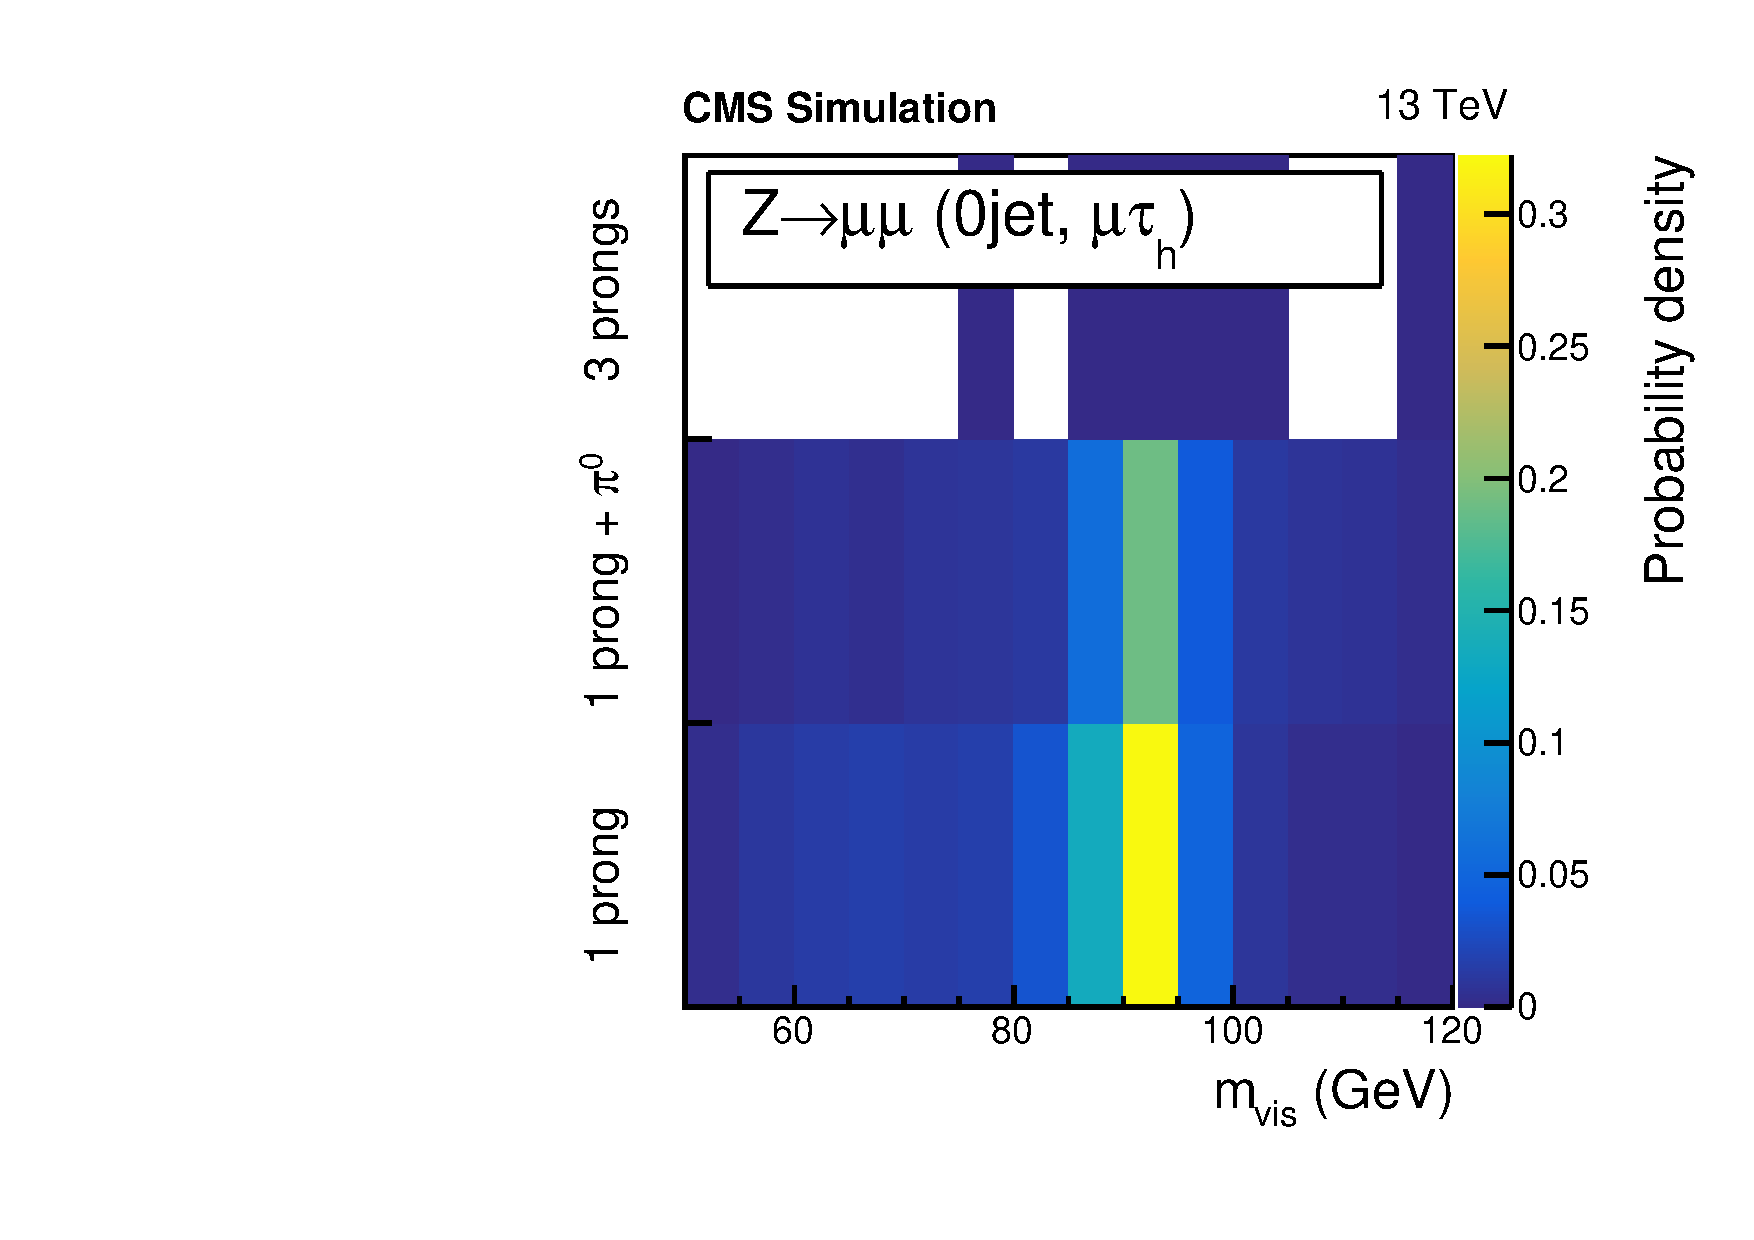
\includegraphics[width=0.4\textwidth]{higgs_to_taus/plots/Figure_001-b.pdf}\\
     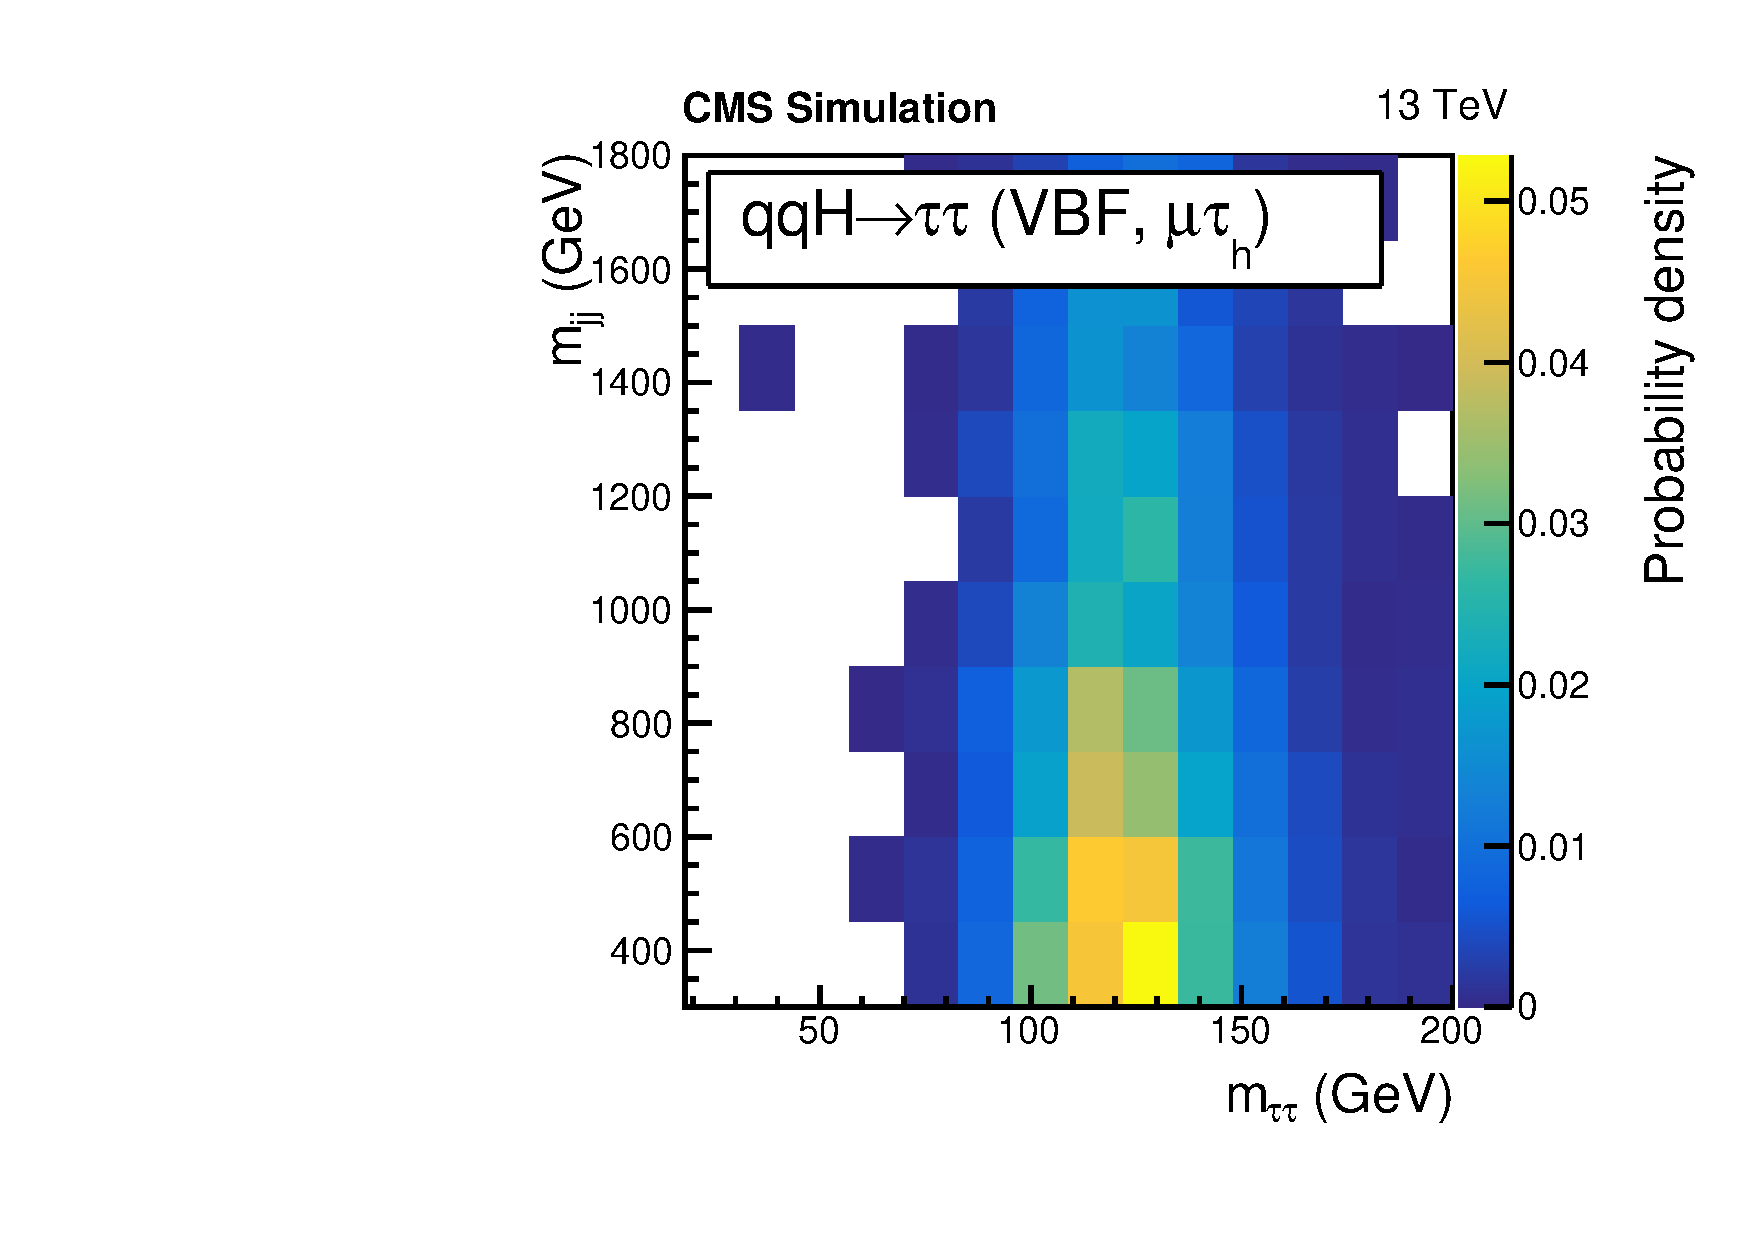
\includegraphics[width=0.4\textwidth]{higgs_to_taus/plots/Figure_001-c.pdf}
     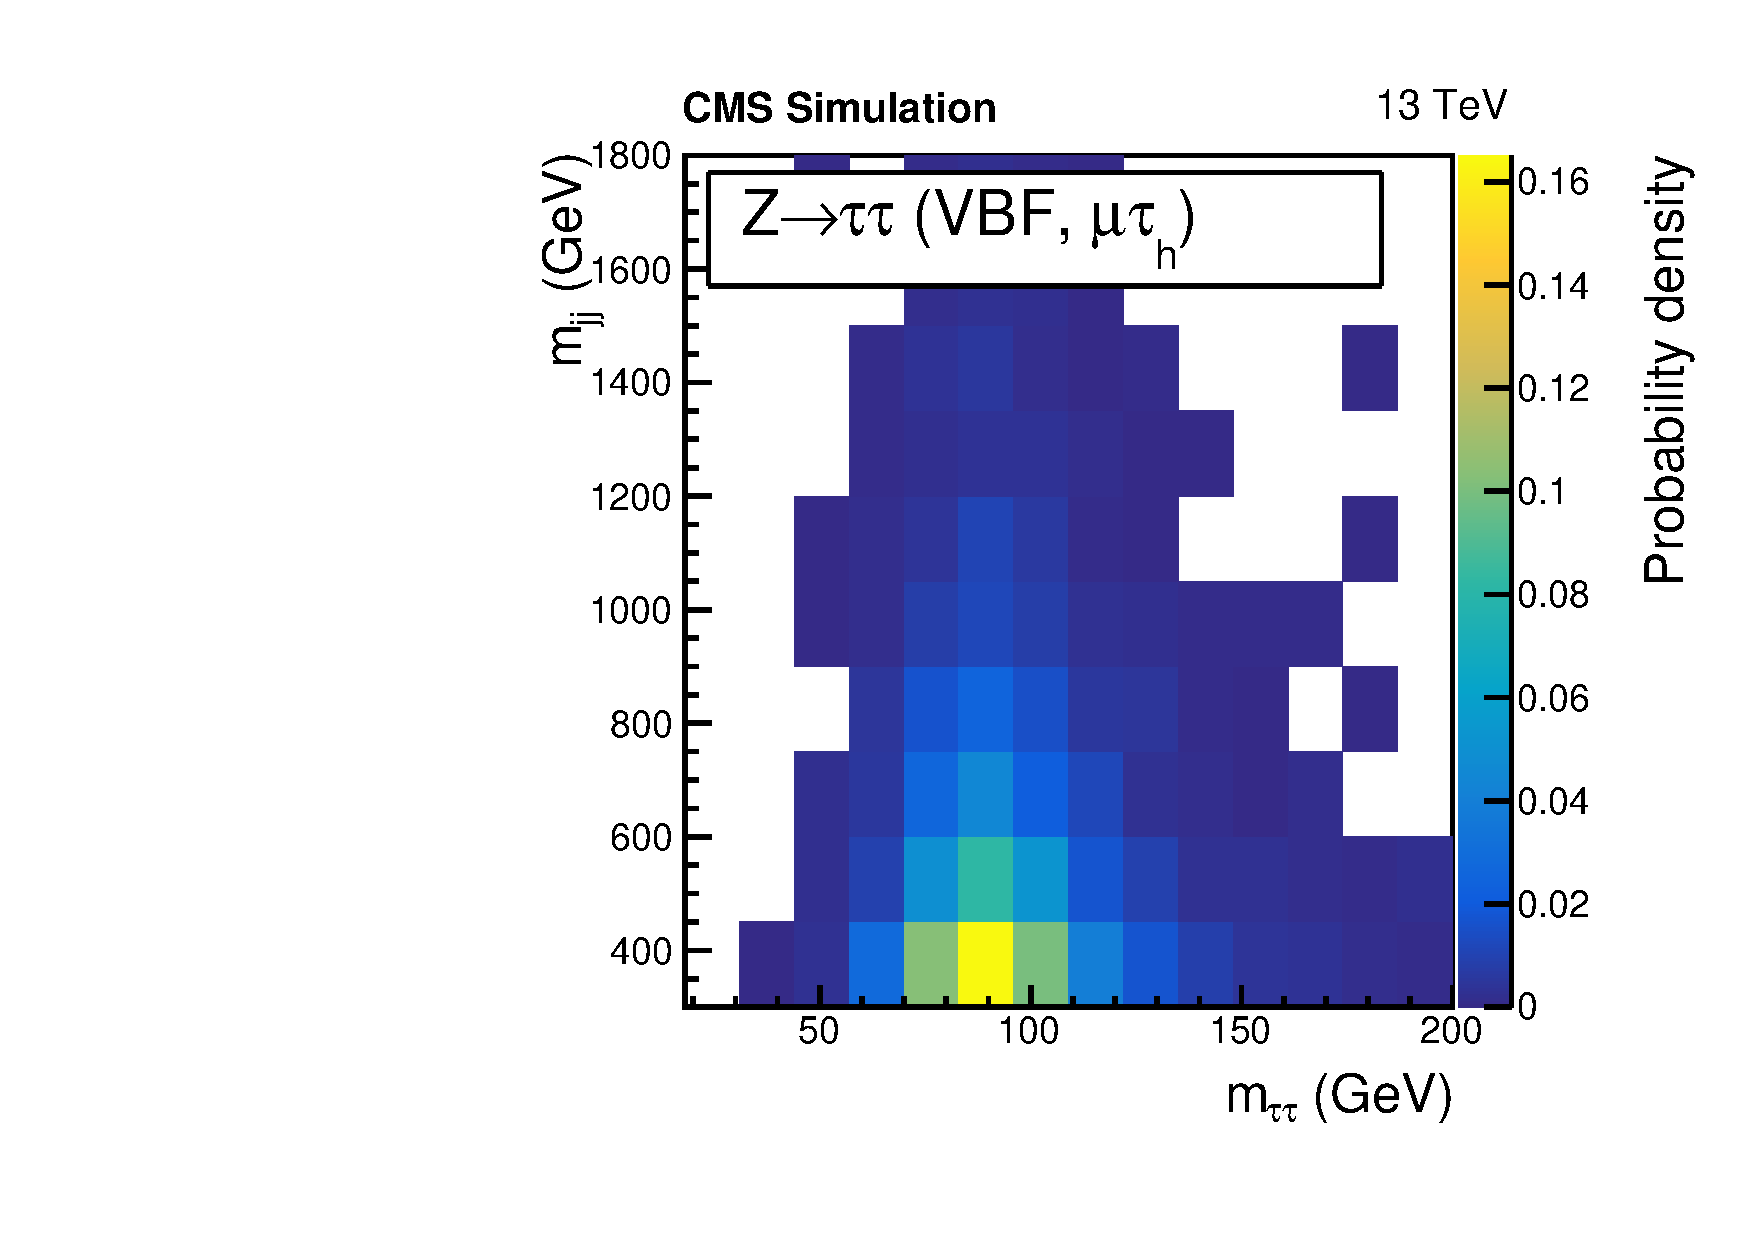
\includegraphics[width=0.4\textwidth]{higgs_to_taus/plots/Figure_001-d.pdf}\\
     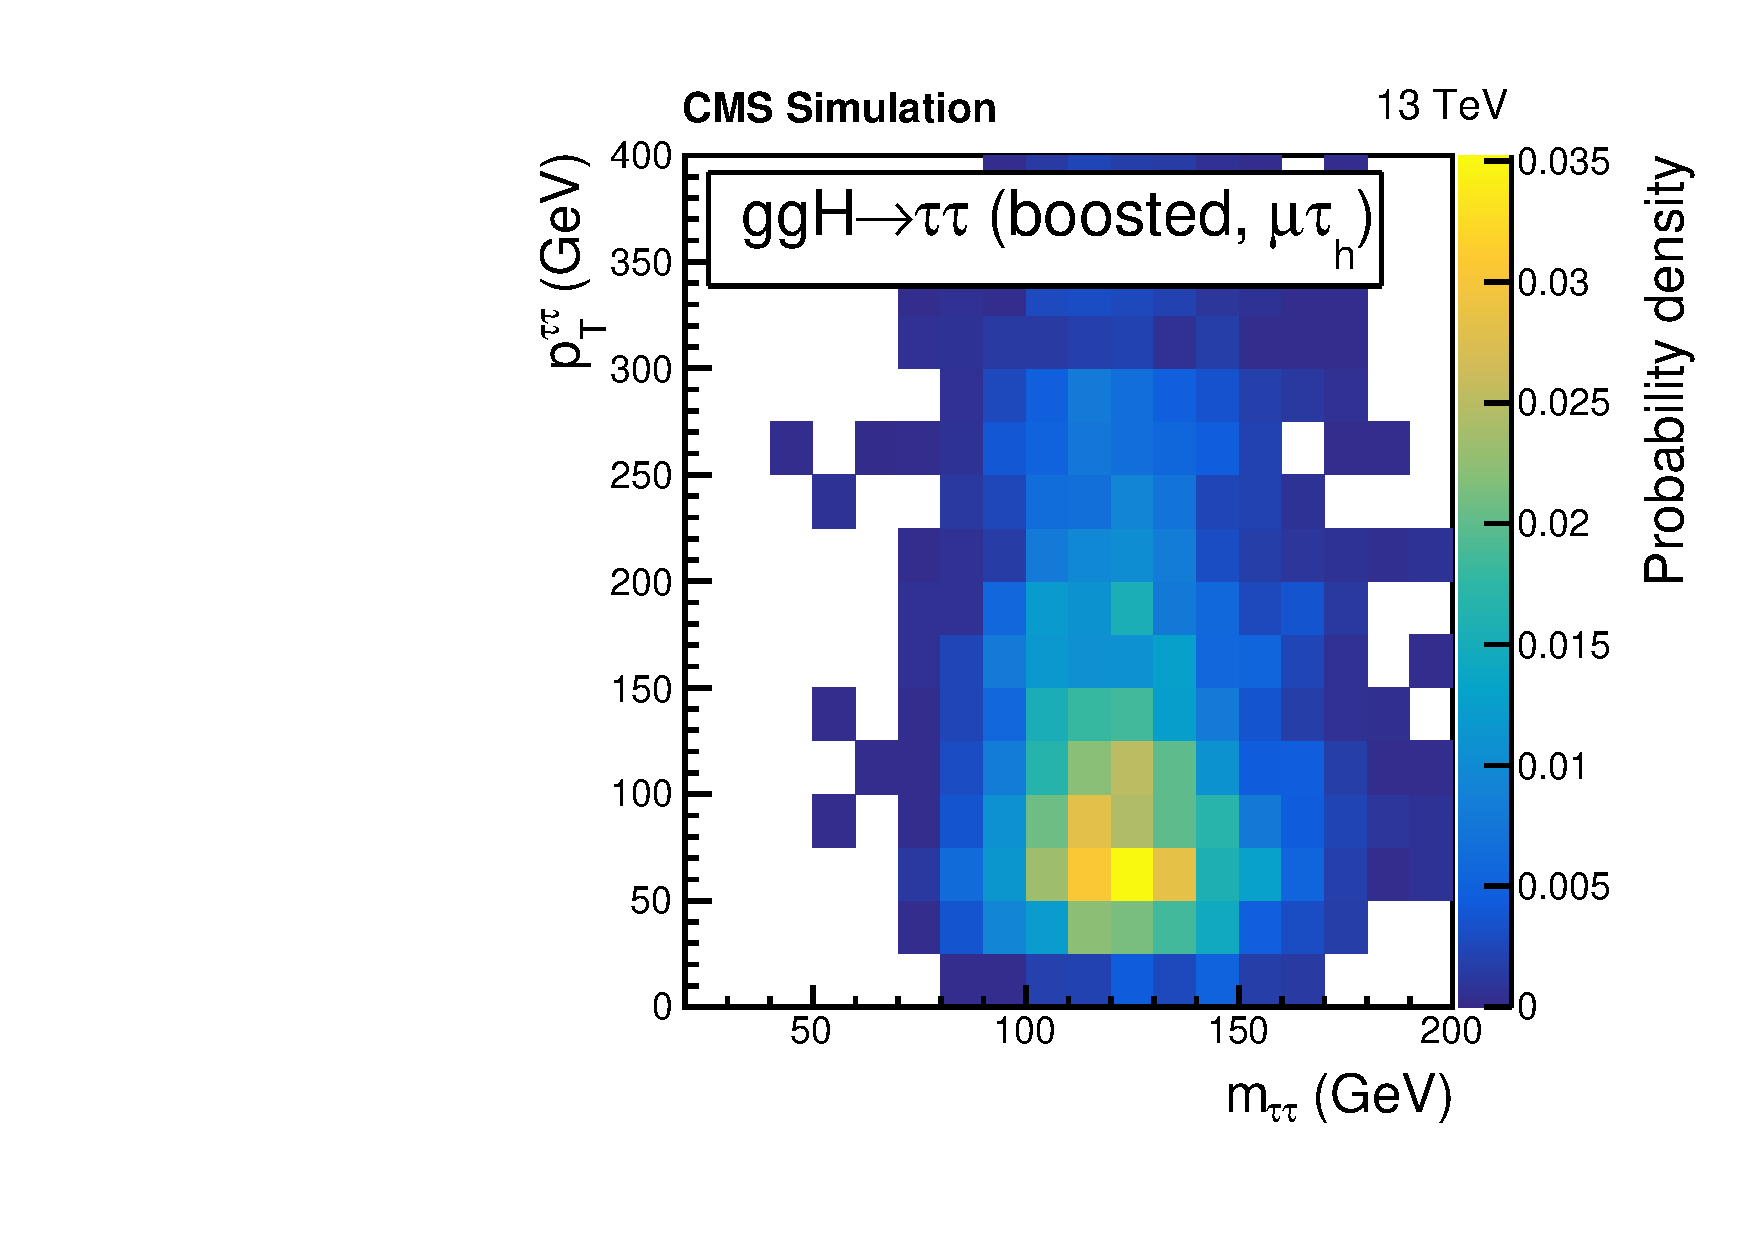
\includegraphics[width=0.4\textwidth]{higgs_to_taus/plots/Figure_001-e.pdf}
     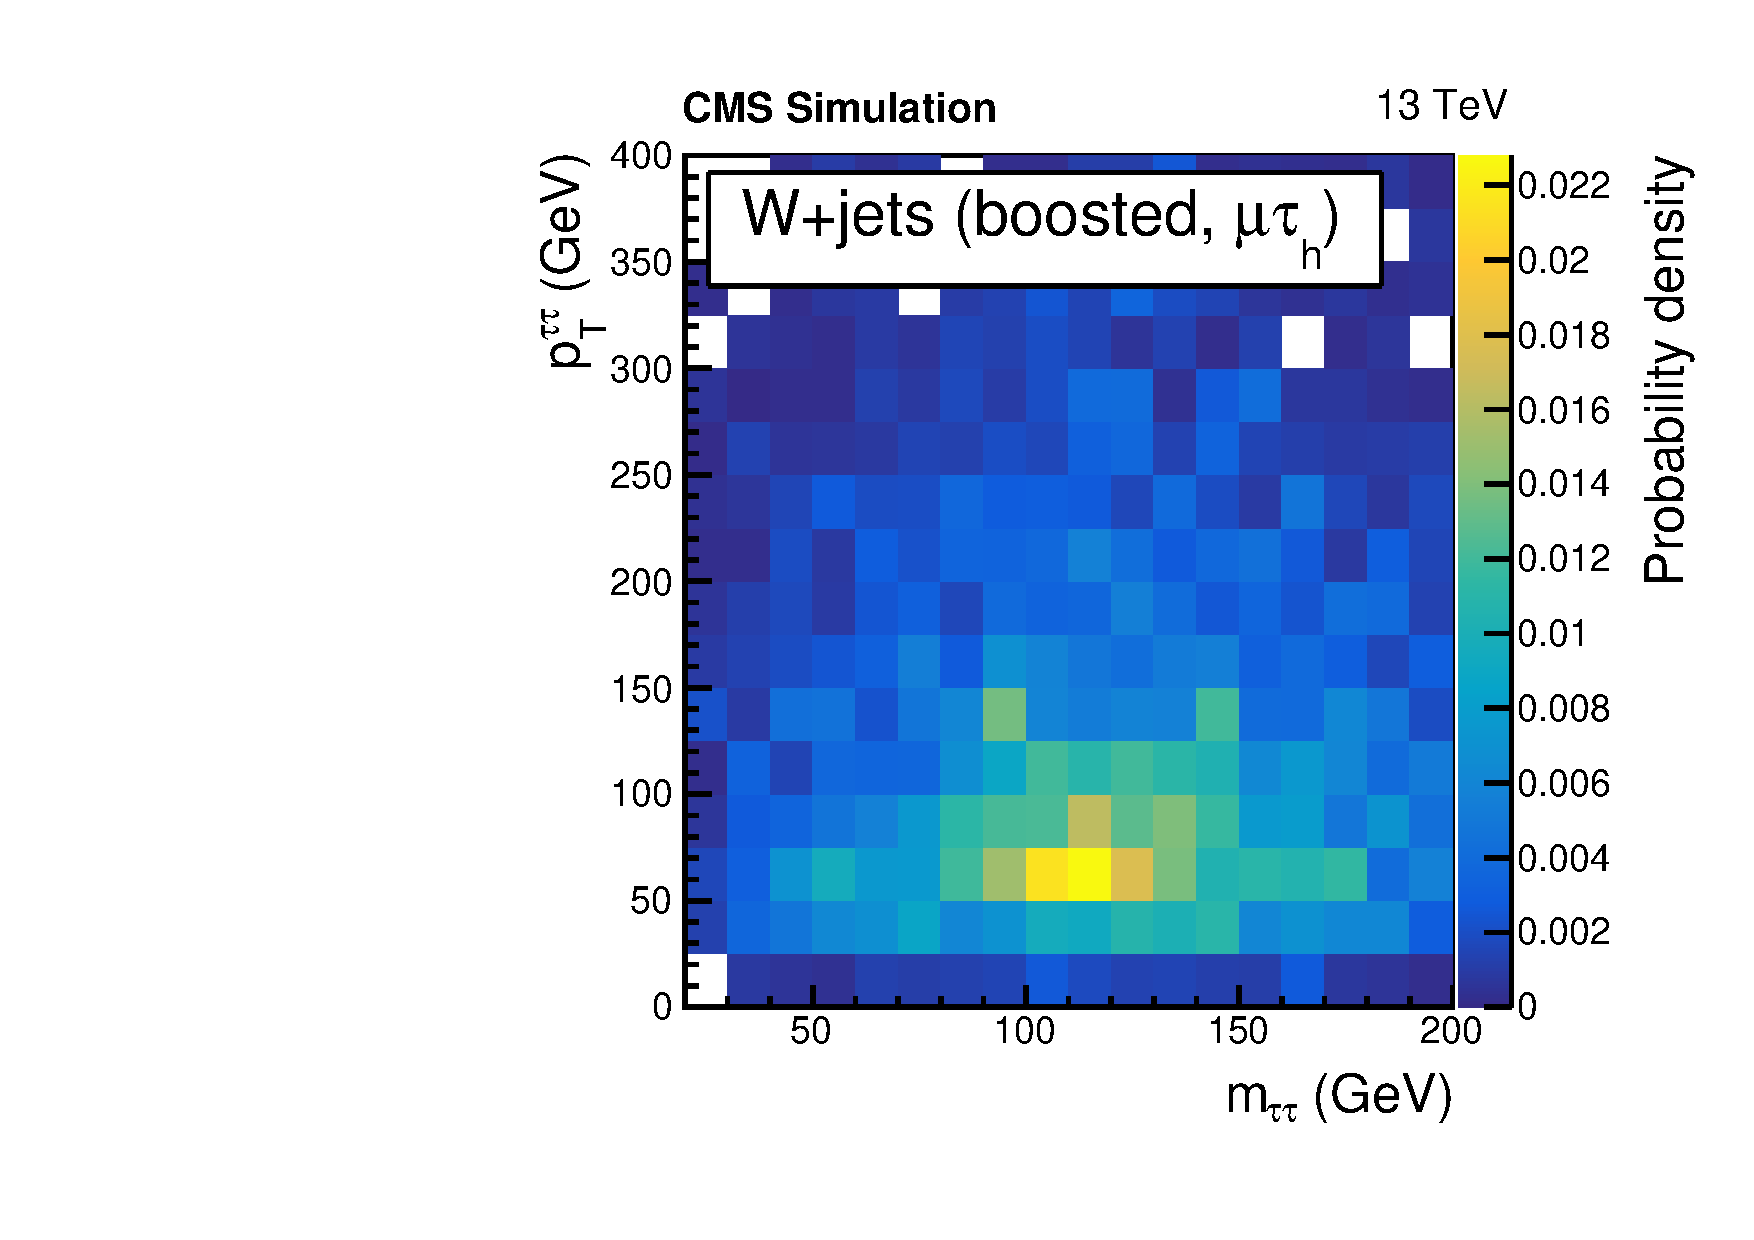
\includegraphics[width=0.4\textwidth]{higgs_to_taus/plots/Figure_001-f.pdf}
     \caption{Two dimensional distributions for Higgs boson events passing event selection 
for each category are shown (left). The specific Higgs boson process shown is the one 
specifically targeted for each category. Distributions for select dominant background 
processes are shown (right). The rows correspond to the three categories: 0-jet (top), 
VBF (center), and Boosted (bottom). All distributions are from the $\Pgm\tauh$ decay channel.} 
\end{figure*}


\begin{table*}
\centering
\begin{small}
\begin{tabular}{llll}
 & 0-jet & VBF & Boosted \\
\hline
 & \multicolumn{3}{c}{Selection} \\ \cline{2-4}
$\tauh\tauh$ & No jet &  \scriptsize{$\geq$2 jets, $\pth>100\GeV$, $\Delta\eta_{\mathrm{jj}}>2.5$} & Others\\
$\Pgm\tauh$ & No jet &  \scriptsize{$\geq$2 jets, $\mjj>300\GeV$, $\pth>50\GeV$, $\pt^{\tauh}>40\GeV$} & Others\\
$\Pe\tauh$ & No jet &  \scriptsize{$\geq$2 jets, $\mjj>300\GeV$, $\pth>50\GeV$} & Others\\
$\Pe\Pgm$ & No jet & \scriptsize{2 jets, $\mjj>300\GeV$} & Others \\
\hline
 & \multicolumn{3}{c}{Observables}\\ \cline{2-4}
$\tauh\tauh$ & $\mtt$                 &    $\mjj$, $\mtt$  &   $\pth$, $\mtt$  \\
$\Pgm\tauh$ & $\tauh$ decay mode, $\mvis$   &    $\mjj$, $\mtt$  &  $\pth$, $\mtt$  \\
$\Pe\tauh$ & $\tauh$ decay mode, $\mvis$   &    $\mjj$, $\mtt$  &  $\pth$, $\mtt$ \\
$\Pe\Pgm$ & $\pt^{\Pgm}$, $\mvis$   &     $\mjj$, $\mtt$  &   $\pth$, $\mtt$  \\
\hline
\end{tabular}
\caption{ Category selection and observables used to build the 2D kinematic distributions. 
The events failing the 0-jet and VBF selection are included in the Boosted category and are
denoted by ``Others''.
\label{tab:htt_categories}
}
\end{small}
\end{table*}

The results of the analysis are extracted with a global maximum likelihood fit based on the 
2D distributions in the various signal regions, and on the control regions, detailed in 
Section~\ref{sec:background_estimation}, that constrain the normalizations of the main backgrounds.

\section{Data Set}
\label{sec:htt_dataset}
The $ggH$ and VBF targeted $\htt$ study utilizes the full 2016 $\pp$ dataset collected by CMS corresponding to 35.9$\fbinv$ 
of integrated luminosity.  The data were gathered at center-of-mass energy 13 TeV.
As data are gathered at CMS, the conditions of the CMS experiment and its subdetectors are recorded.
The CMS experiment uses an offline validation process to ensure that only high quality
data is used in future analyses.  Data collected while the CMS detector is in a faulty state
is flagged as such and skipped. The CMS experiment collected 35.9$\fbinv$ of integrated 
lumiosity worth of data usable for physics analysis in 2016.

In this analysis only a subset of the total data marked as good is used.  During data
gathering, data is filtered into primary datasets (PDs) corresponding to which HLT trigger
made the determination to save a given event.  The HLT triggers using in this analysis,
detailed in table~\ref{tab:htt_hlt_triggers}, correspond to: the Single Electron/Photon
PD, the Single Muon PD, the Muon and Electron PD, and the Tau PD.



\section{Monte Carlo Samples}
\label{sec:htt_mc_samples}
Signal and background processes are modeled with samples of simulated events.
For details on the production for simulated events, see section~\ref{sec:simulation}.

The signal samples with a Higgs boson produced vai the gluon fusion production
mechanism ($\cPg\cPg\PH$), vector boson fusion (VBF), or in association with a $\PW$ or $\PZ$ boson ($\PW\PH$ or $\PZ\PH$), 
are generated at next-to-leading order (NLO) in perturbative quantum chromodynamics (pQCD) 
with the \POWHEG 2.0~\cite{Nason:2004rx,Frixione:2007vw, Alioli:2010xd, Alioli:2010xa, Alioli:2008tz} 
generator. For the $\PW\PH$ and $\PZ\PH$ simulated samples, the \textsc{minlo hvJ}~\cite{Luisoni:2013kna} 
extension of \POWHEG 2.0 is used. The set of parton distribution functions (PDFs) used for all
simulated samples is NNPDF30\_nlo\_as\_0118~\cite{Ball:2011uy}. It is found that the $\ttbar\PH$ 
process is negligible in comparison with the other signal processes and is therefor excluded.
Mass dependant production cross sections and $\htt$ branching fractions for the SM Higgs boson production, 
and their corresponding uncertainties are taken from 
Refs.~\cite{deFlorian:2016spz,Denner:2011mq,Ball:2011mu} and references therein.

The \MGAMCNLO~\cite{Alwall:2014hca} generator is used for $\PZ+$jets and $\PW+$jets processes. 
They are simulated at leading order (LO) with MLM jet matching and merging~\cite{Alwall:2007fs}.
The \MGAMCNLO generator is also used for diboson production simulated at next-to-LO (NLO) with the 
FxFx jet matching and merging~\cite{Frederix:2012ps}. In contrast, \POWHEG 2.0 and 1.0 are used for \ttbar
and single top quark production, respectively. The generators are interfaced with \PYTHIA 
8.212 ~\cite{Sjostrand:2014zea} to model the parton showering and fragmentation, as well as 
the decay of the $\Pgt$ leptons. The \PYTHIA parameters affecting the description of the 
underlying event are set to the {CUETP8M1} tune~\cite{Khachatryan:2015pea}.

For each simulated event, a number of additional pileup interactions is simulated and added. 
The number of pileup interactions added is based on best efforts to match the simulated
events to the pileup in data which is estimated from the measured instantaneous
luminosity for each bunch crossing. The average number of additional pileup interactions in
the 2016 CMS data is approximately 27 interactions per bunch crossing.


\section{SVFit Algorithm}
\label{sec:svfit}
FIXME -- need to edit this part
The visible mass of the $\Pgt\Pgt$ system, $\mvis$, can be used to separate
the $\PH\to \Pgt \Pgt$ signal events
from the large contribution of irreducible $\PZ \to \Pgt \Pgt$ events.
However, the neutrinos from the $\Pgt$ lepton decays carry a large fraction of
the $\Pgt$ lepton energy and reduce the discriminating power of this variable.
The \textsc{svfit} algorithm combines the \etvecmiss with the four-vectors of both $\Pgt$ candidates
to calculate a more accurate estimate of the mass of the parent boson, denoted as $\mtt$. The resolution of $\mtt$ is between 15 and 20\% depending on the $\Pgt\Pgt$ final state.
A detailed description of the algorithm can be found
in Ref.~\cite{Bianchini:2014vza}. Both variables are used in the analysis, as detailed in Section.~\ref{sec:categories}, and $\mvis$ is preferred over $\mtt$ when the background from $\PZ \to \ell\ell$ events is large.


\section{Background Estimation}
\label{sec:background_estimation}
\subsubsection{Drell--Yan Background}
The largest irreducible source of background is the Drell--Yan production
of $\PZ/\Pgg^*\to\Pgt\Pgt, \ell\ell$. Proper shape and normalization for this
leading background is critical to the success of the analysis.
A dedicated, high purity, $\PZ/\Pgg^*\to\Pgm\Pgm$ control region was
used to measure reweighting factors for application to all Drell--Yan
simulated events and is detailed in the Monte Carlo Corrections 
section~\ref{sec:htt_dy_reweighting}.

\subsubsection{$\PW+\text{jets}$ Background}
The $\PW+\text{jets}$ process is modelled using simulation.
In the $\tauh\tauh$ and $\Pe\Pgm$ channels the $\PW+\text{jets}$ contribution 
is small compared to other backgrounds. In these two channels both the shape and 
yield are taken from simulation.
The background from $\PW+\text{jets}$ production contributes significantly to the
$\Pgm\tauh$ and $\Pe\tauh$ channels, when the $\PW$ boson decays leptonically and
a jet is misidentified as a $\tauh$ candidate. In the $\ell\tauh$ channels
the shape of the background is from simulation. The yield is estimated 
using data in a $\PW+\text{jets}$ enriched dedicated side-band region defined
based on a transverse mass cut, $\MT > 80\GeV$. In this high-$\MT$ side-band region, the $\PW+\text{jets}$
process is scaled so that the sum total of expected background events is equivalent
to the sum total of observed data events. The scaling factor is then applied
in the low transverse mass signal regions, $\MT < 50\GeV$. A scaling factor
is measured for the 0-jet and Boosted categories for both $\Pe\Pgt$ and $\Pgm\Pgt$ resulting
in four $\PW+\text{jets}$ scaling values. The scaling factor measured in the Boosted
category is extrapolated to the VBF category. The $\PW+\text{jets}$ purity in these
side-band regions varies from about 50\% in the Boosted category to 85\% in the 0-jet category.

The high-$\MT$ side-bands, described above, are included as control regions in the final fit.
These high-$\MT$ $\PW+\text{jets}$ control regions can be seed in Figure~\ref{fig:htt_wj_CR1}.
The control regions are only a singular bin because they are used solely to constrain 
the normalization of the $\PW+\text{jets}$ process.

\begin{figure*}[!htbp]
\centering
     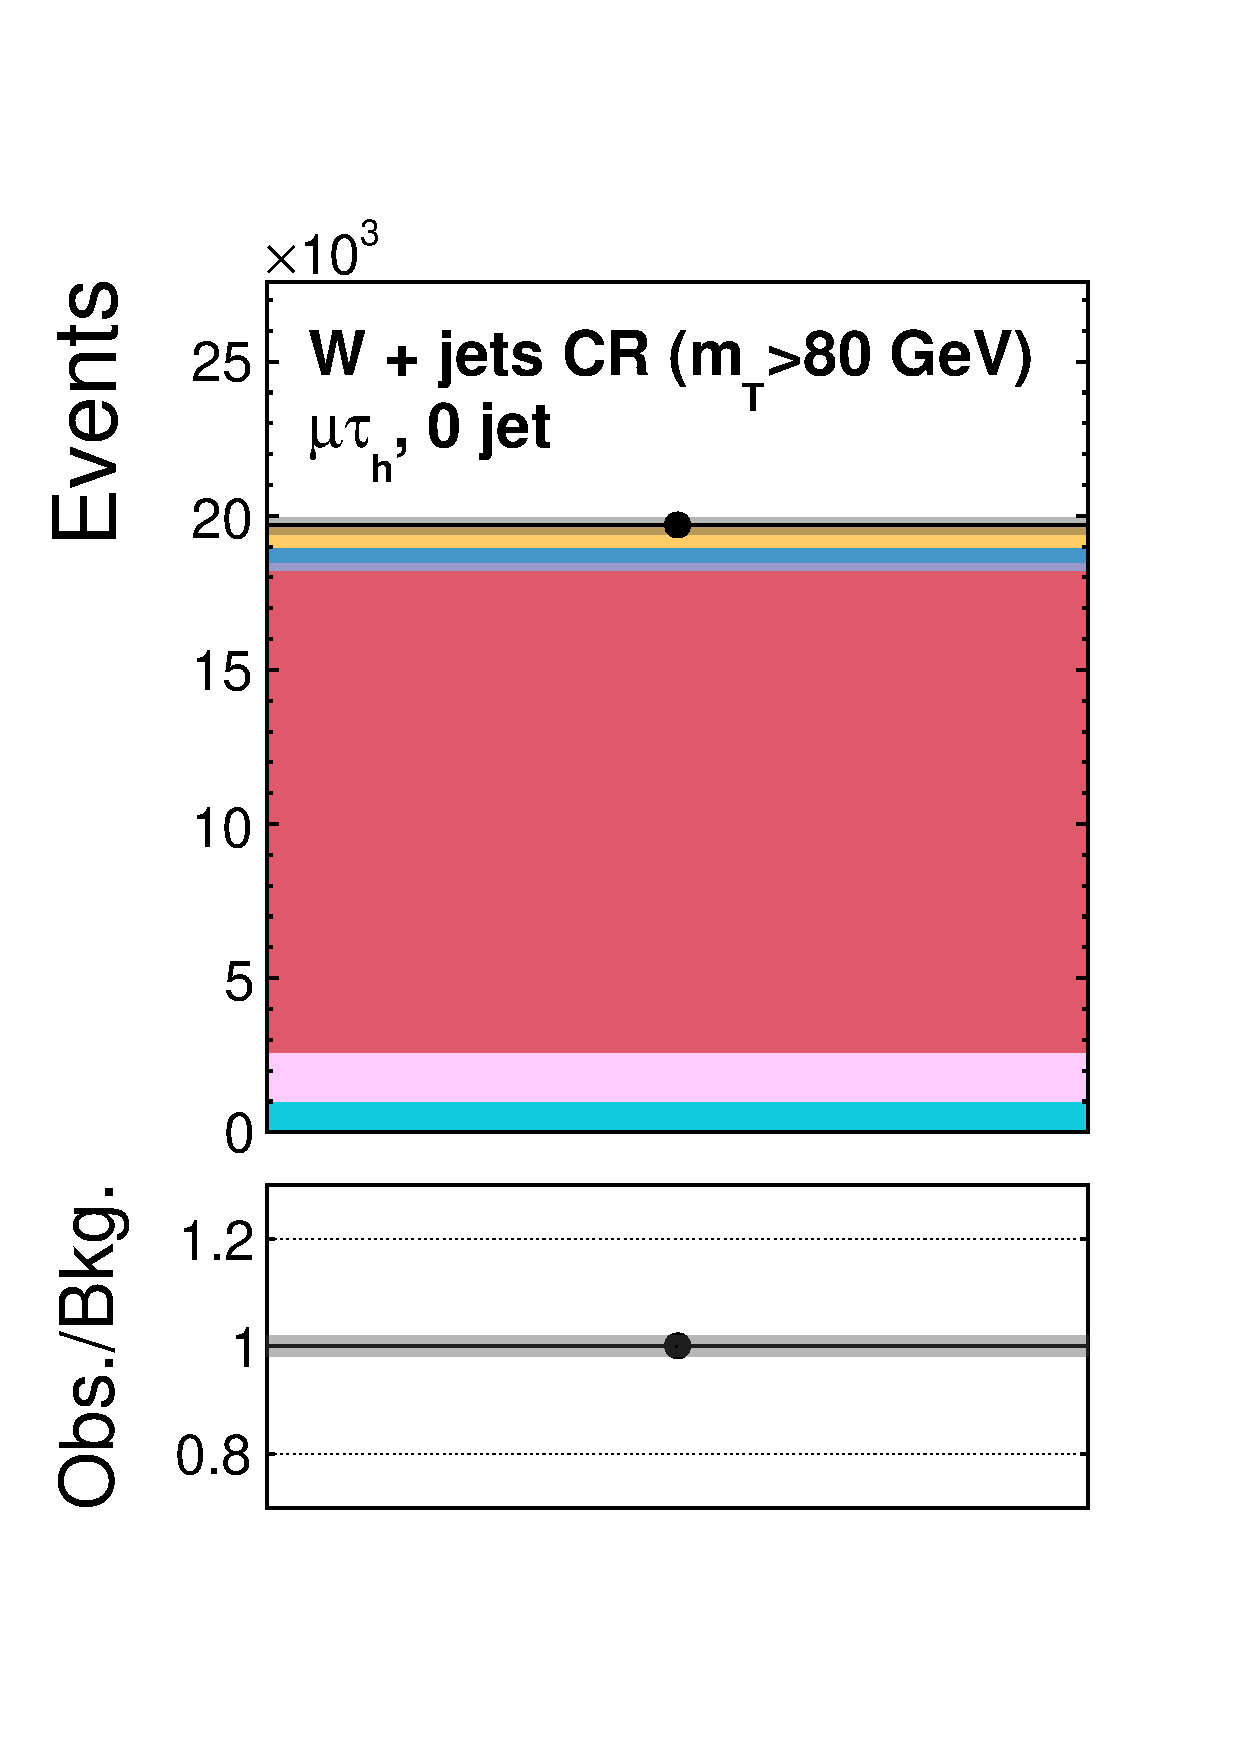
\includegraphics[width=0.19\textwidth]{higgs_to_taus/plots/Figure_002-a.pdf}
     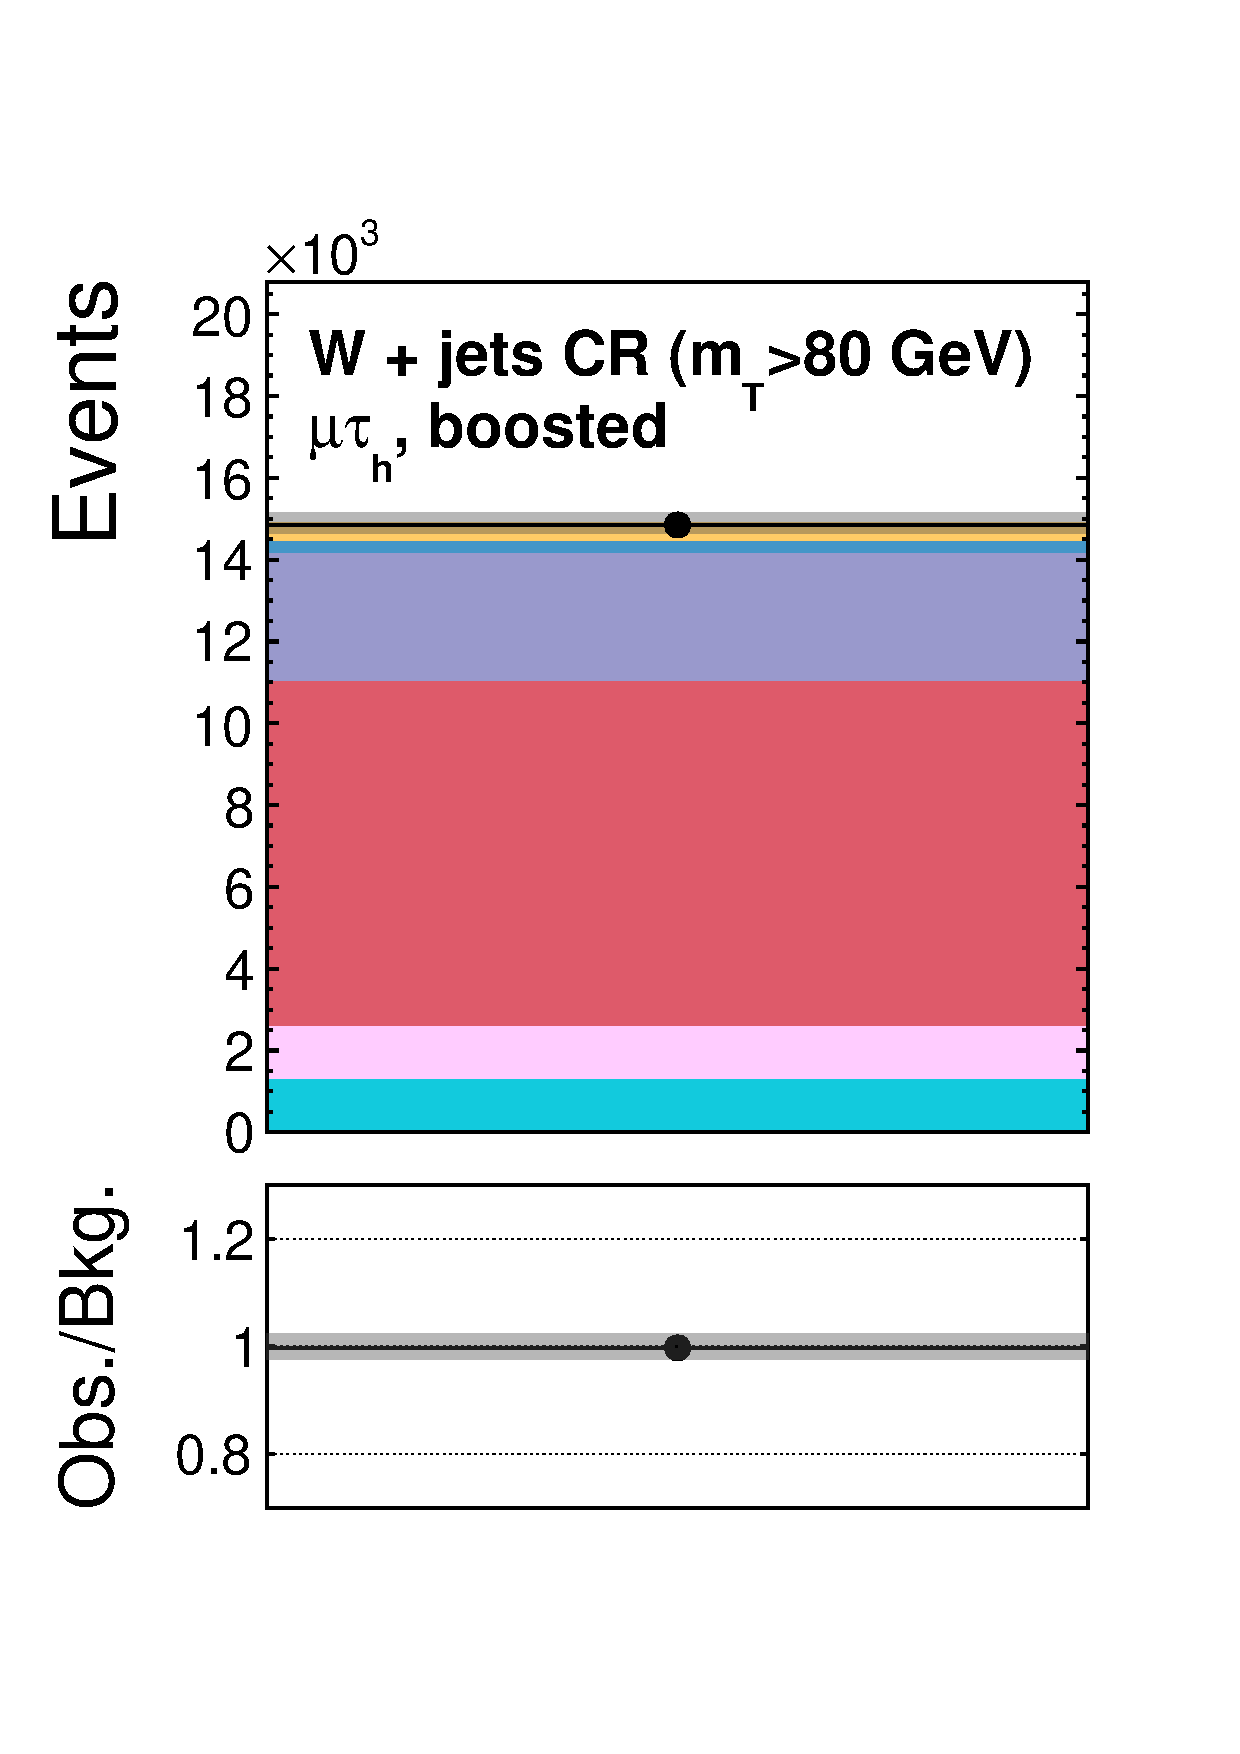
\includegraphics[width=0.19\textwidth]{higgs_to_taus/plots/Figure_002-b.pdf}
     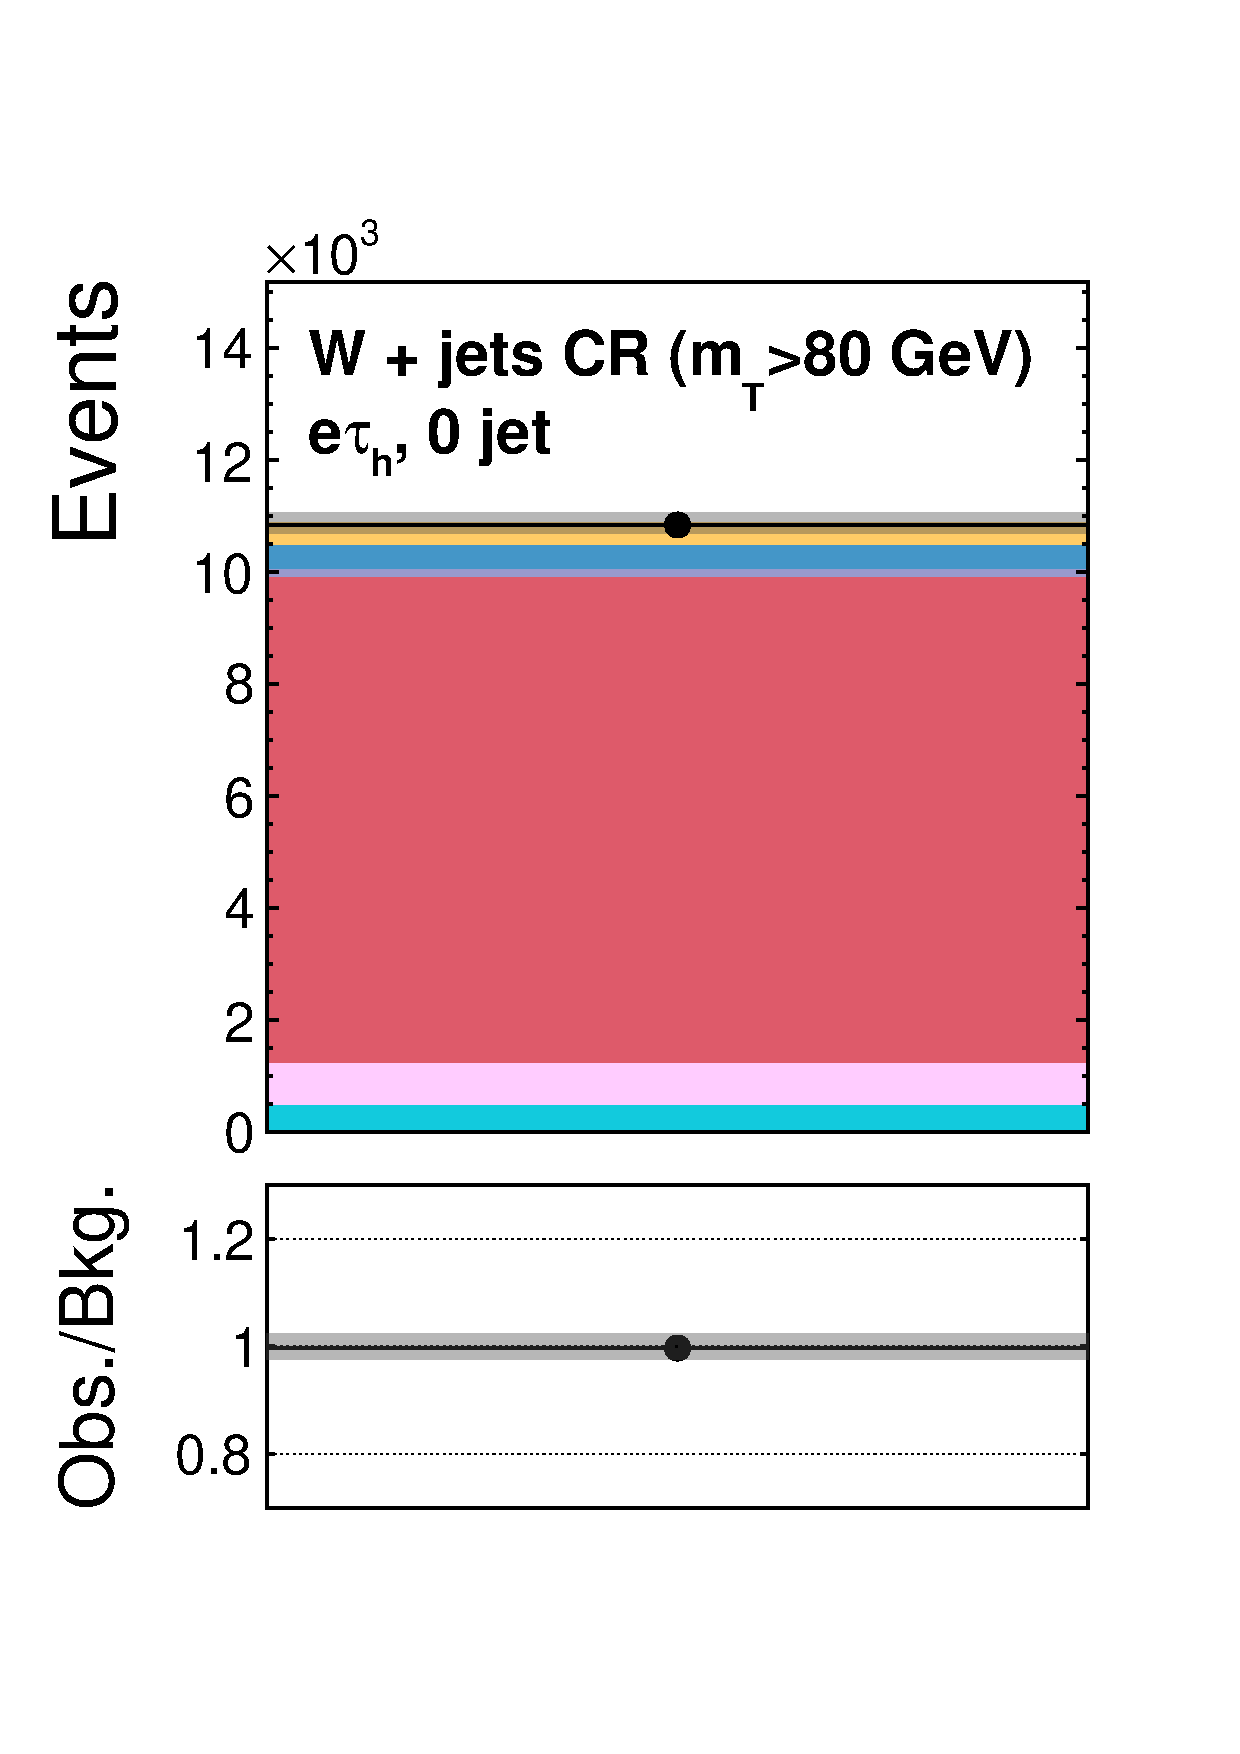
\includegraphics[width=0.19\textwidth]{higgs_to_taus/plots/Figure_002-c.pdf}
     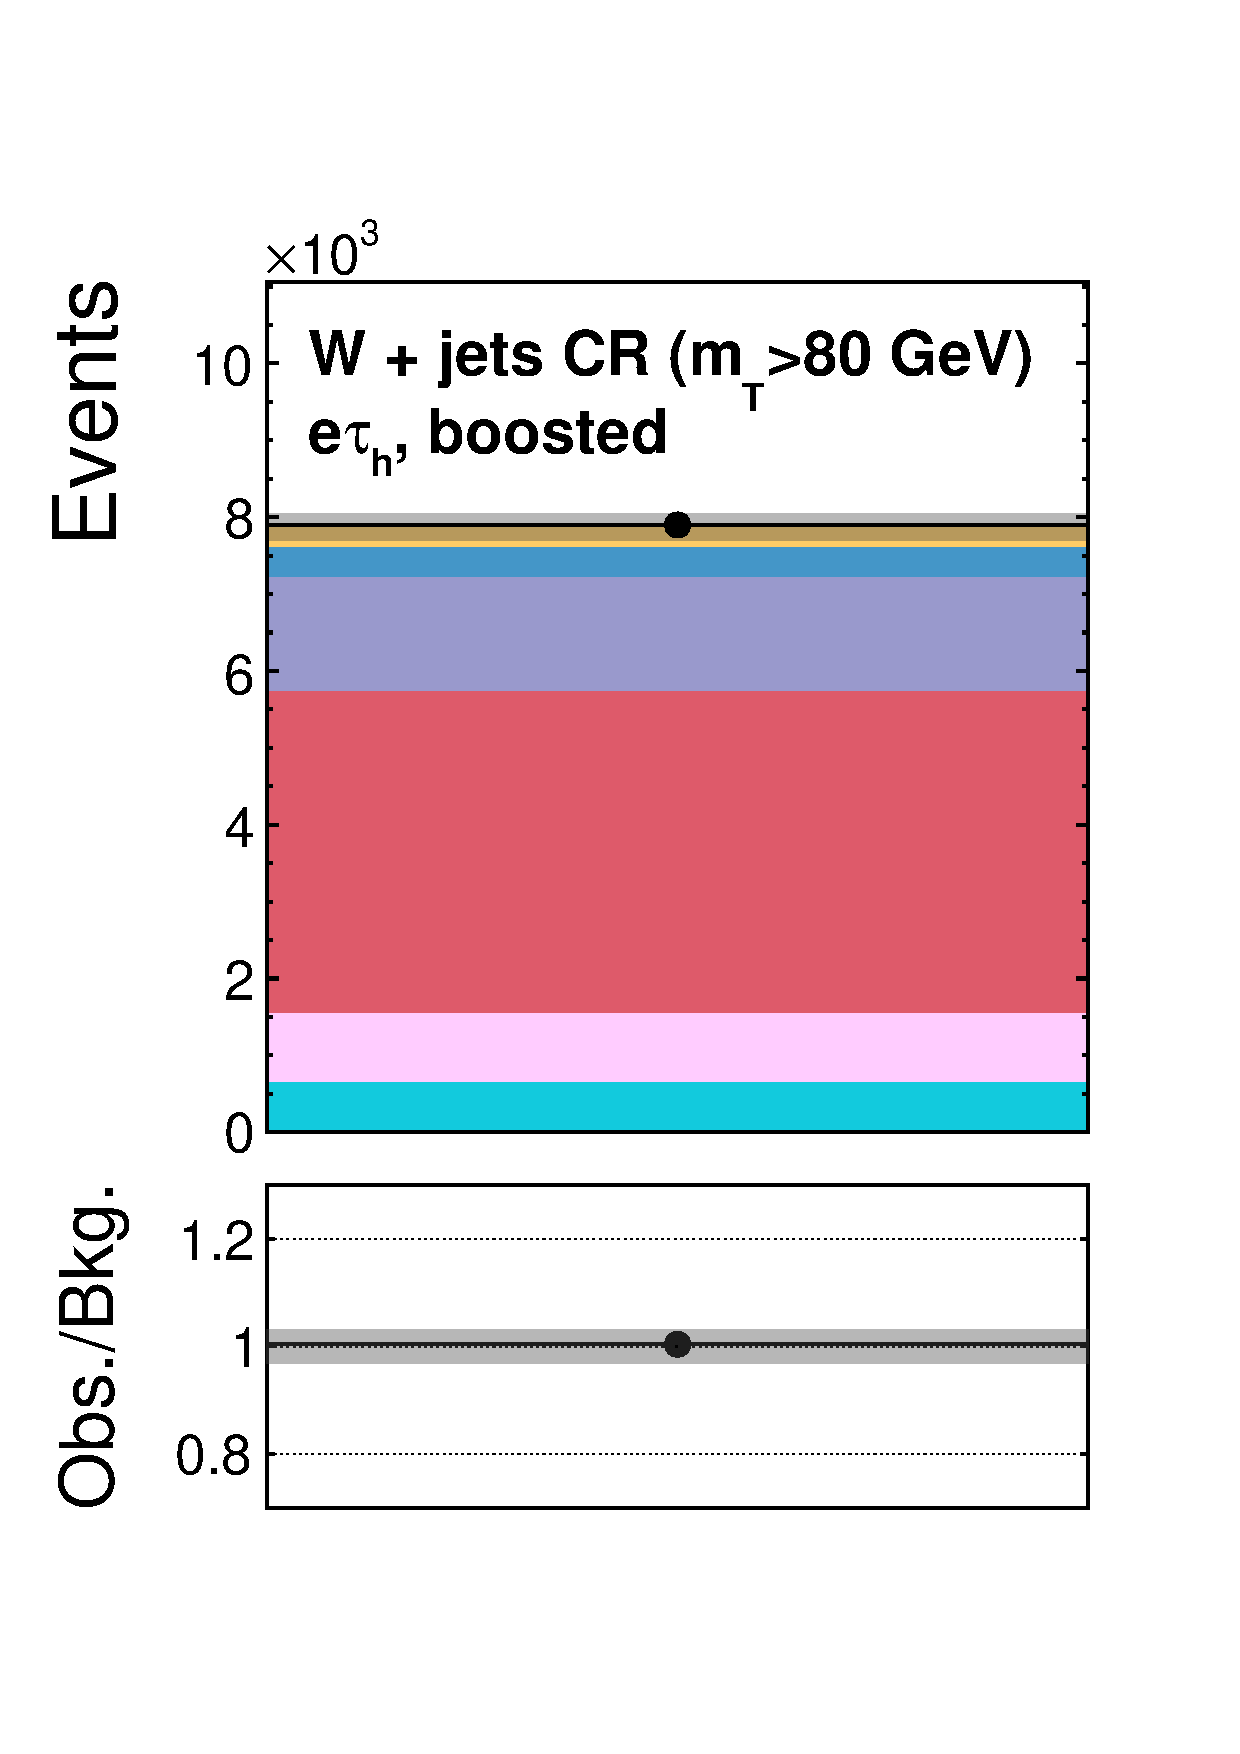
\includegraphics[width=0.19\textwidth]{higgs_to_taus/plots/Figure_002-d.pdf}
     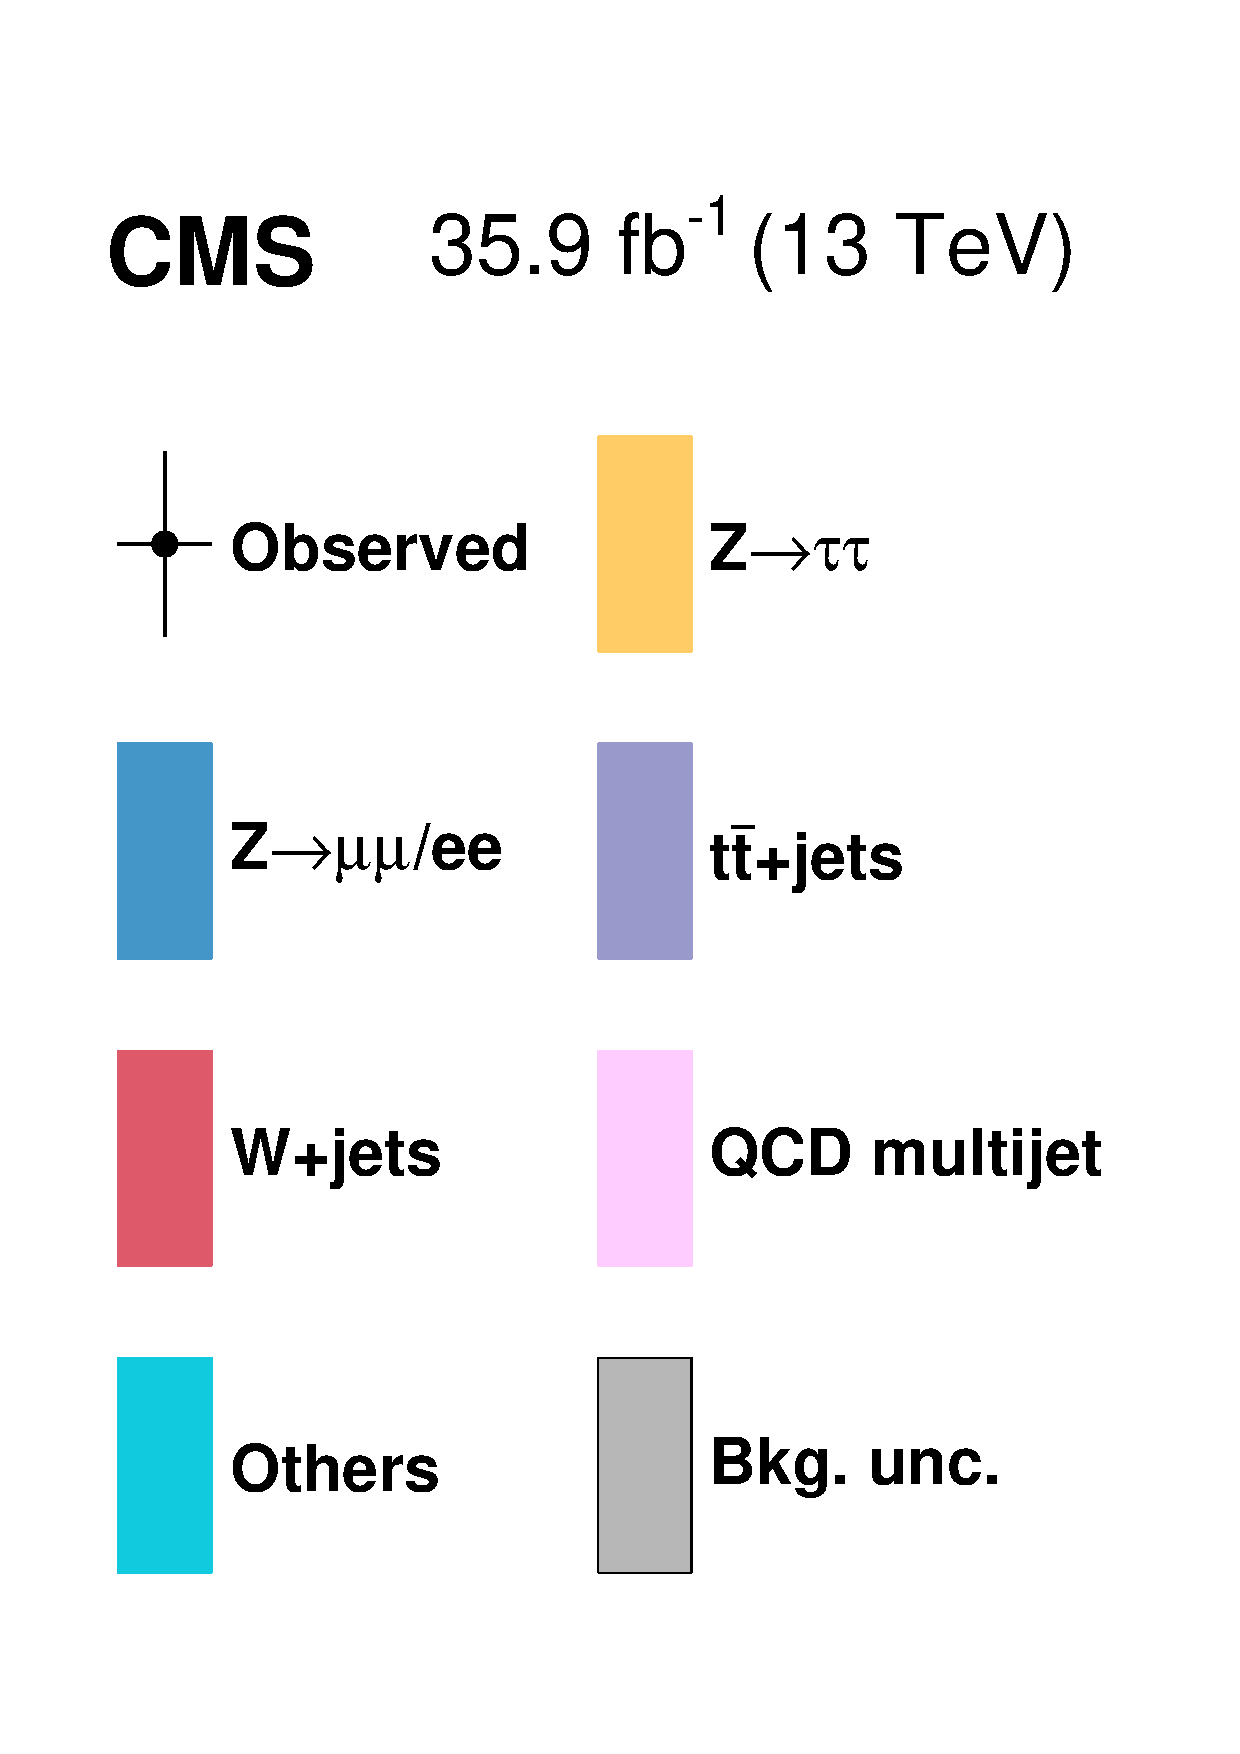
\includegraphics[width=0.19\textwidth]{higgs_to_taus/plots/Figure_002-e.pdf}
     \caption{the high-$\MT$ control regions enriched in the $\PW+\text{jets}$ background used in 
the maximum likelihood fit, together with the signal regions, to extract the results. 
The normalization of the predicted background distributions corresponds to the result of 
the global fit. These regions, defined with $\MT>80$\GeV, control the yields of the 
$\PW+\text{jets}$ background in the $\Pgm\tauh$ and $\Pe\tauh$ channels.  
}
     \label{fig:htt_wj_CR1}
\end{figure*}


\subsubsection{QCD Multijet Background}
The QCD multijet process constitutes an important source of reducible background 
in the $\tauh\tauh$ and $\ell\tauh$ channels. The QCD multijet process is subdominant
in the $\Pe\Pgm$ channel. For all four channels, the QCD multijet, is estimated from data.  
Side-band control regions are constructed to estimate the shape and the yield of the QCD multijet 
background in these channels.

QCD multijet estimation for the $\ell\tauh$ channels follows:
\begin{enumerate}

\item Raw yield is extracted using a sample where the
$\ell$ and the $\tauh$ candidates have the same-sign charge. Using this sample, the QCD multijet 
process is estimated from data by subtracting the contribution of the Drell--Yan, \ttbar, diboson,
and $\PW+\text{jets}$ processes as in equation~\ref{eqn:qcd_eqn}.
\begin{equation}
\label{eqn:qcd_eqn}
\text{QCD} = \text{Data} - \text{Other Background Processes}
\end{equation}

\item The 2D distributions of the QCD multijet background are estimated from a region with 
same-sign leptons, same as the yield estimate, except the isolation of the $\ell$ and $\tauh$ 
candidates is additionally relaxed to reduce the statistical fluctuations in the distributions. 
The contributions from other background process are subtracted from data, equation~\ref{eqn:qcd_eqn},
to extract the QCD multijet shape template in this region.

\item The raw yield obtained above is corrected to account for observed differences between the background 
composition in the same-sign and opposite-sign regions. An extrapolation factor between the same-sign 
and opposite-sign regions is determined by comparing the yield of the estimated QCD multijet background for 
events with $\ell$ candidates passing inverted isolation criteria, in the same-sign and opposite-sign 
regions. This extrapolation factor is allowed to adjust in the final fit via the inclusion of dedicated QCD
multijet control regions for these channels.
%Figure~\ref{fig:htt_qcd_CR3} shows these control regions for the 0-jet and Boosted categories 
%of the $\Pgm\tauh$ and $\Pe\tauh$ channels; the observable is $\mvis$ or $\mtt$ to provide 
%discrimination between the QCD multijet and the $\PZ\to\Pgt\Pgt$ processes.
\end{enumerate}

The same technique is used in the $\Pe\Pgm$ channel, except no control region is included in the 
fit because QCD multijet events contribute little to the total background in this decay channel.

%\begin{figure*}[!htbp]
%\centering
%     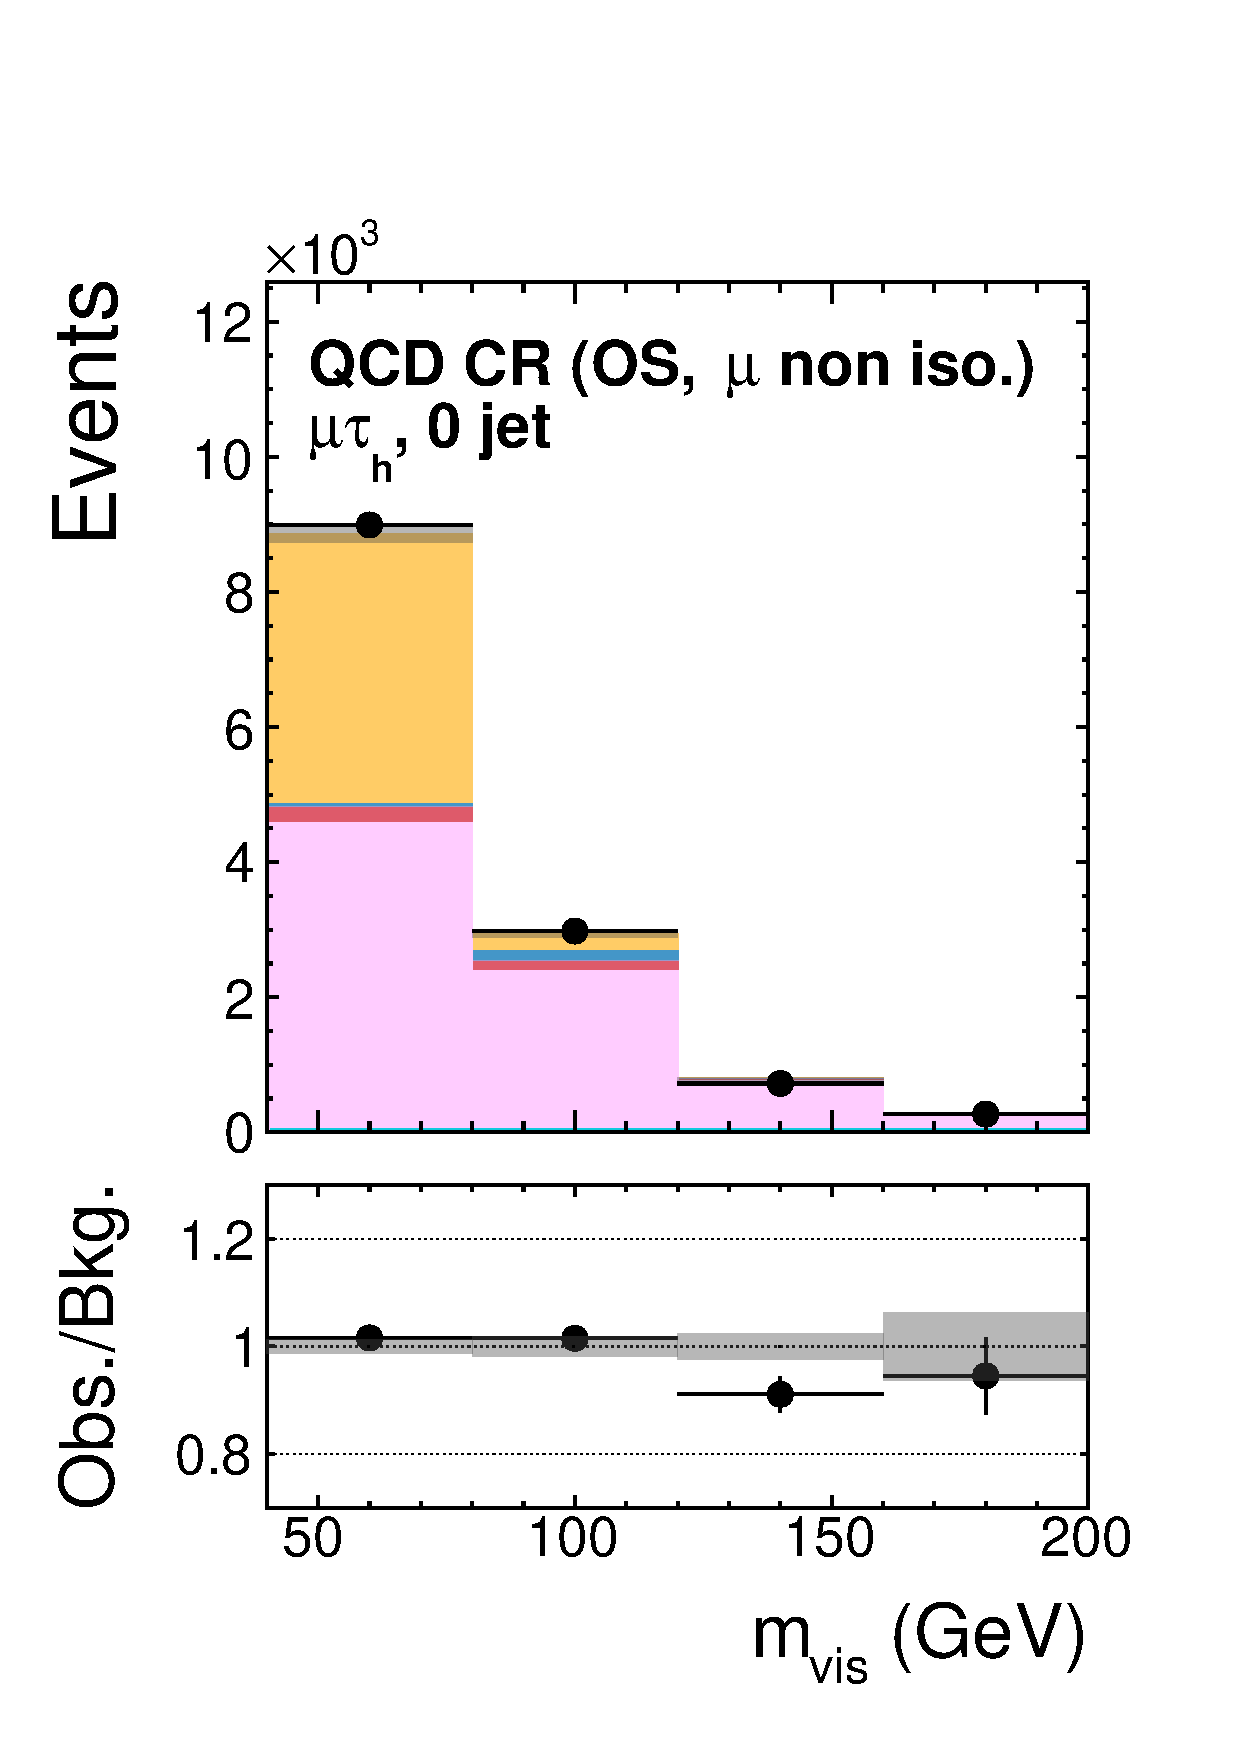
\includegraphics[width=0.3\textwidth]{higgs_to_taus/plots/Figure_003-a.pdf}
%     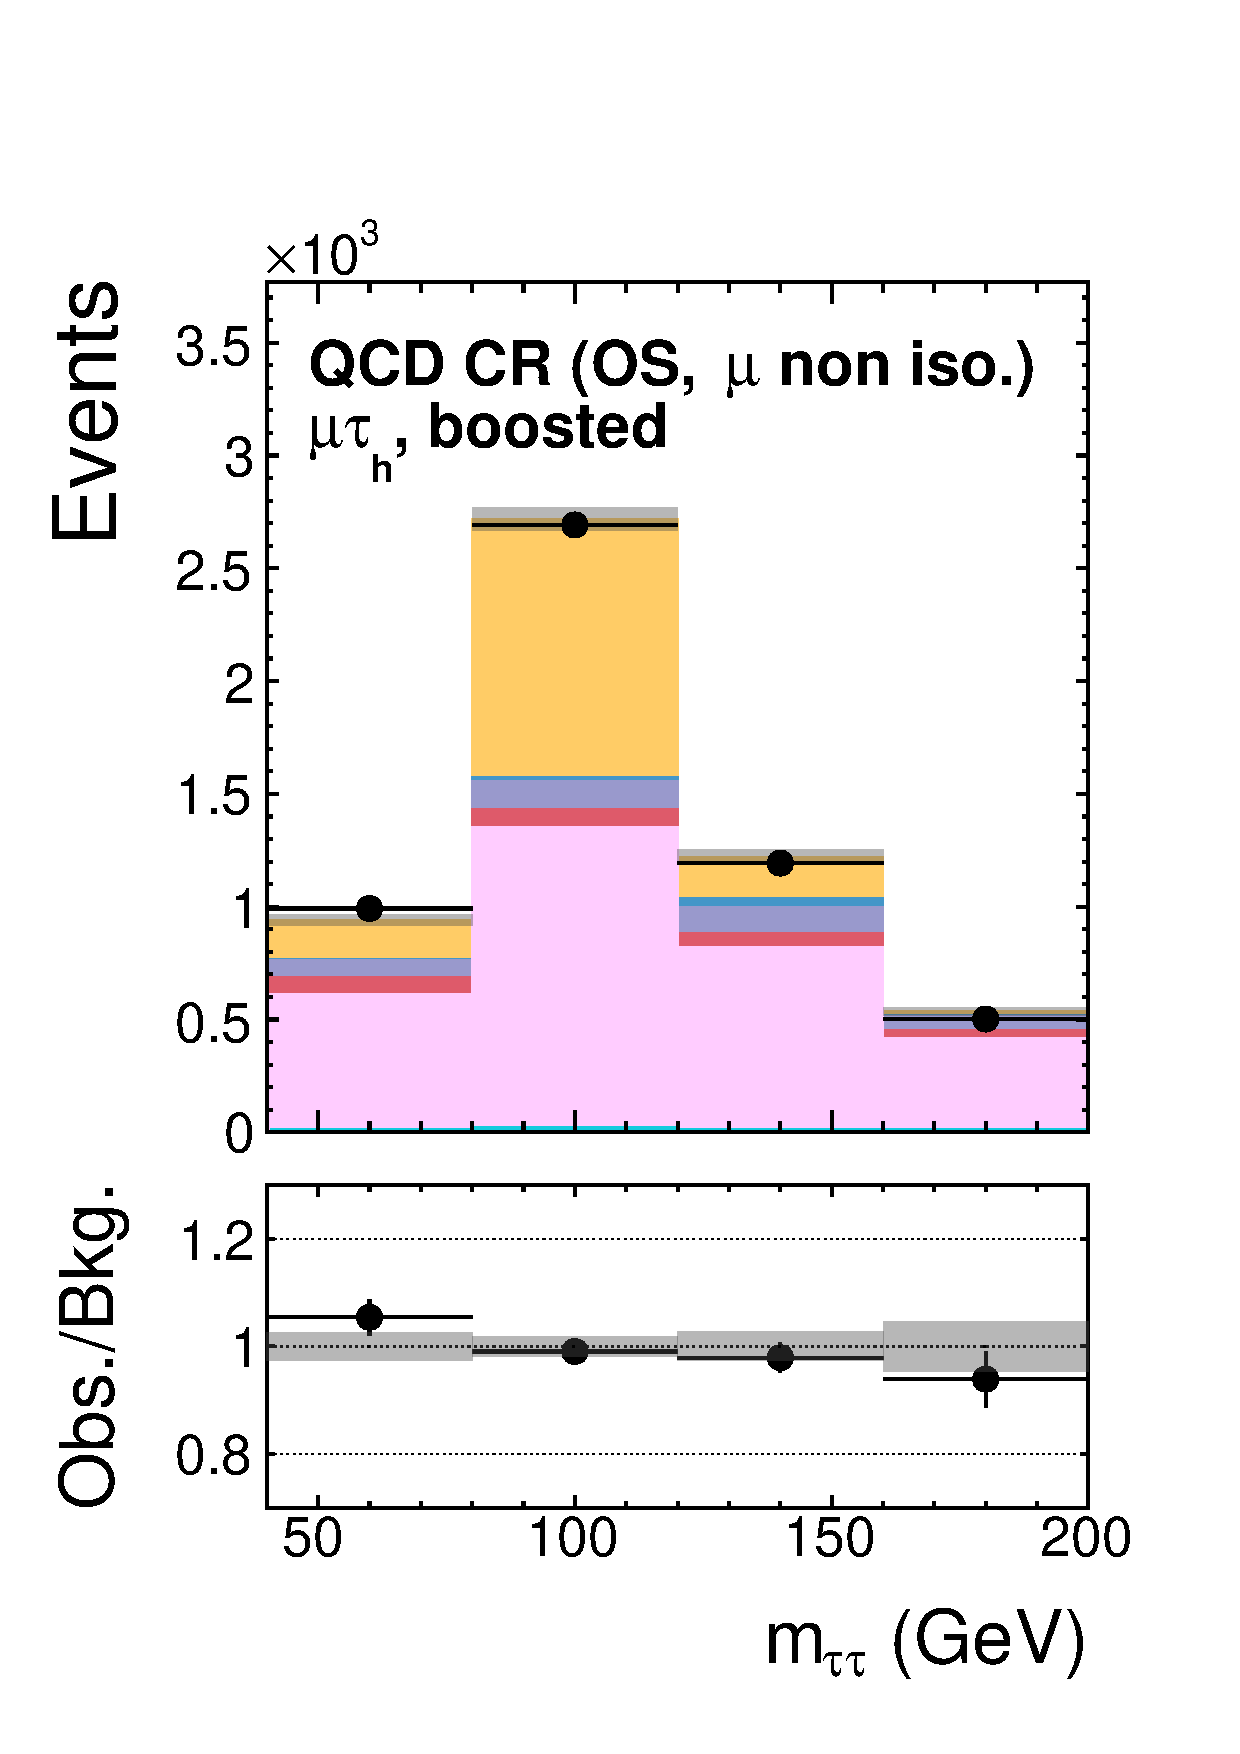
\includegraphics[width=0.3\textwidth]{higgs_to_taus/plots/Figure_003-b.pdf}
%     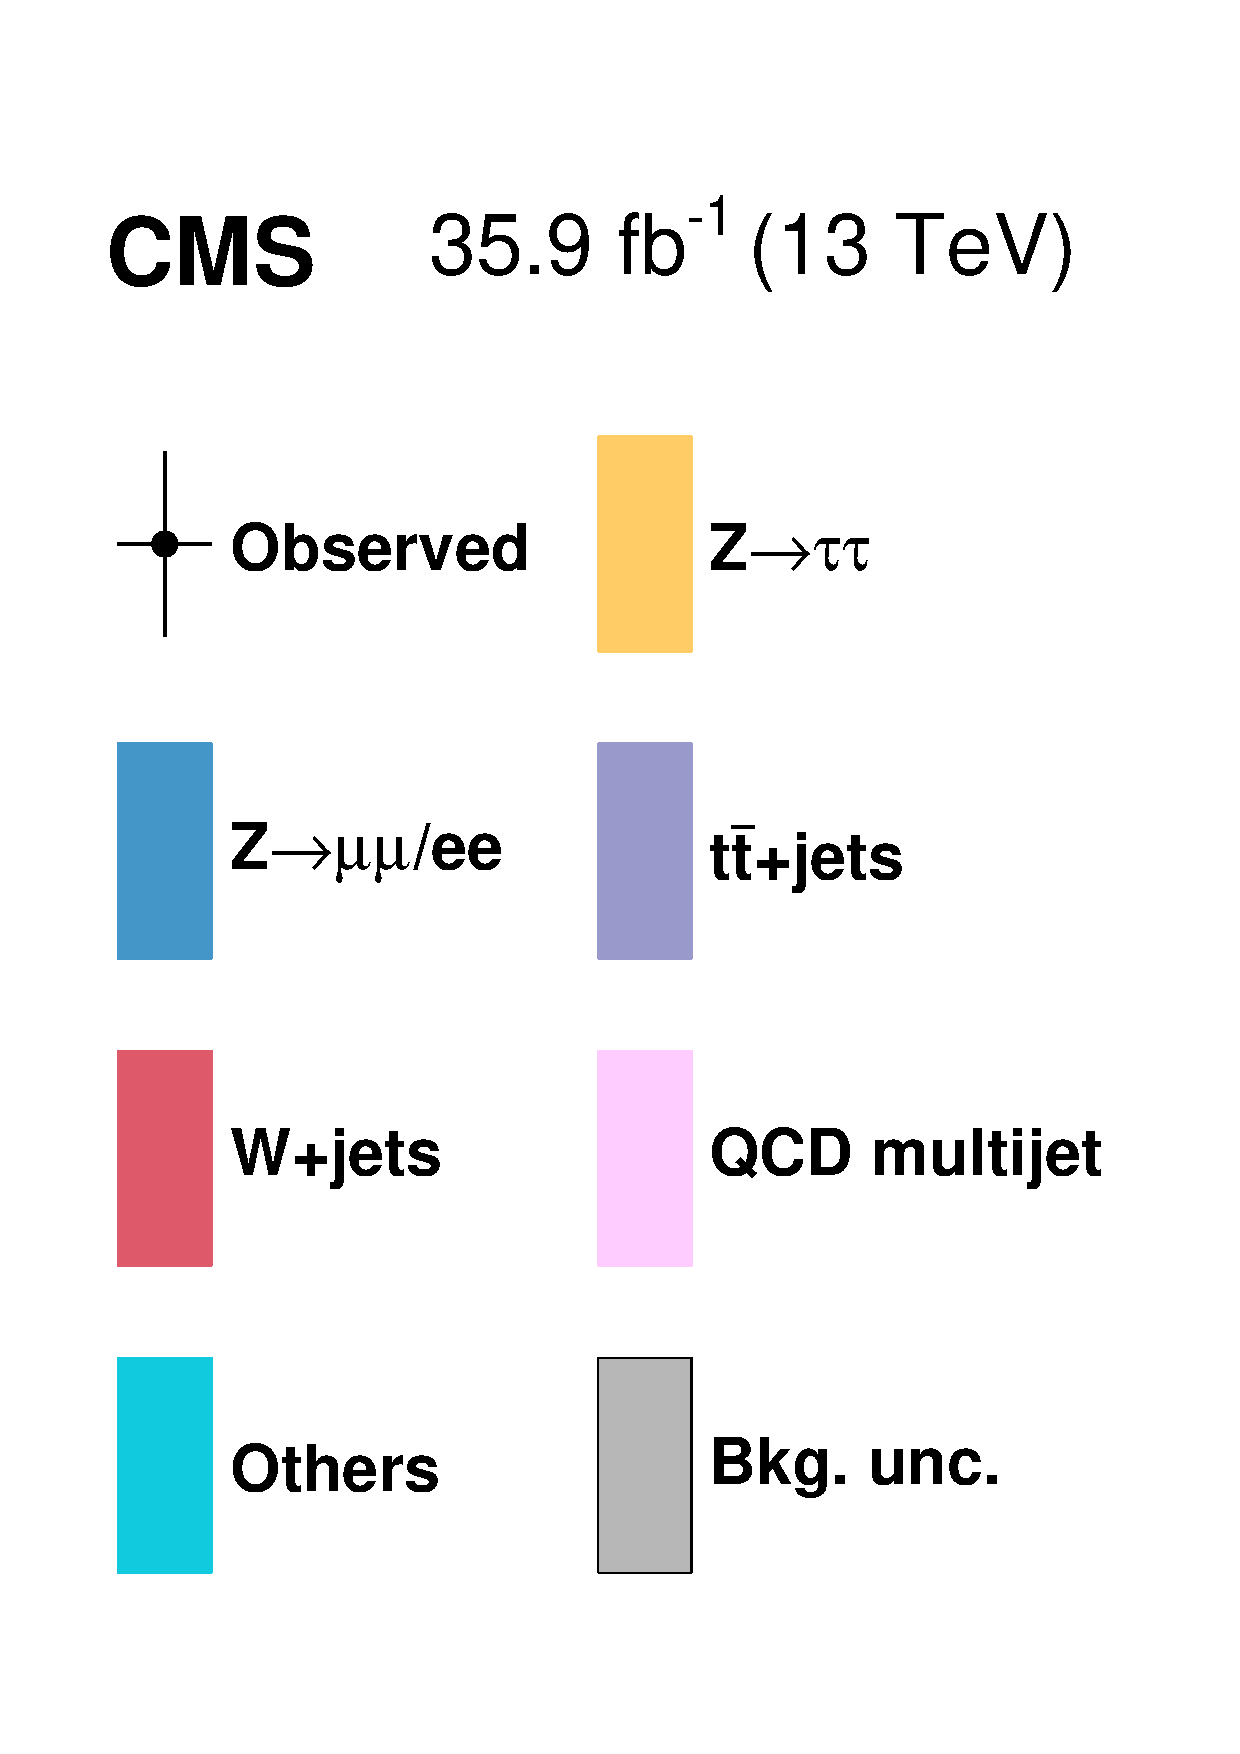
\includegraphics[width=0.3\textwidth]{higgs_to_taus/plots/Figure_003-c.pdf}
%     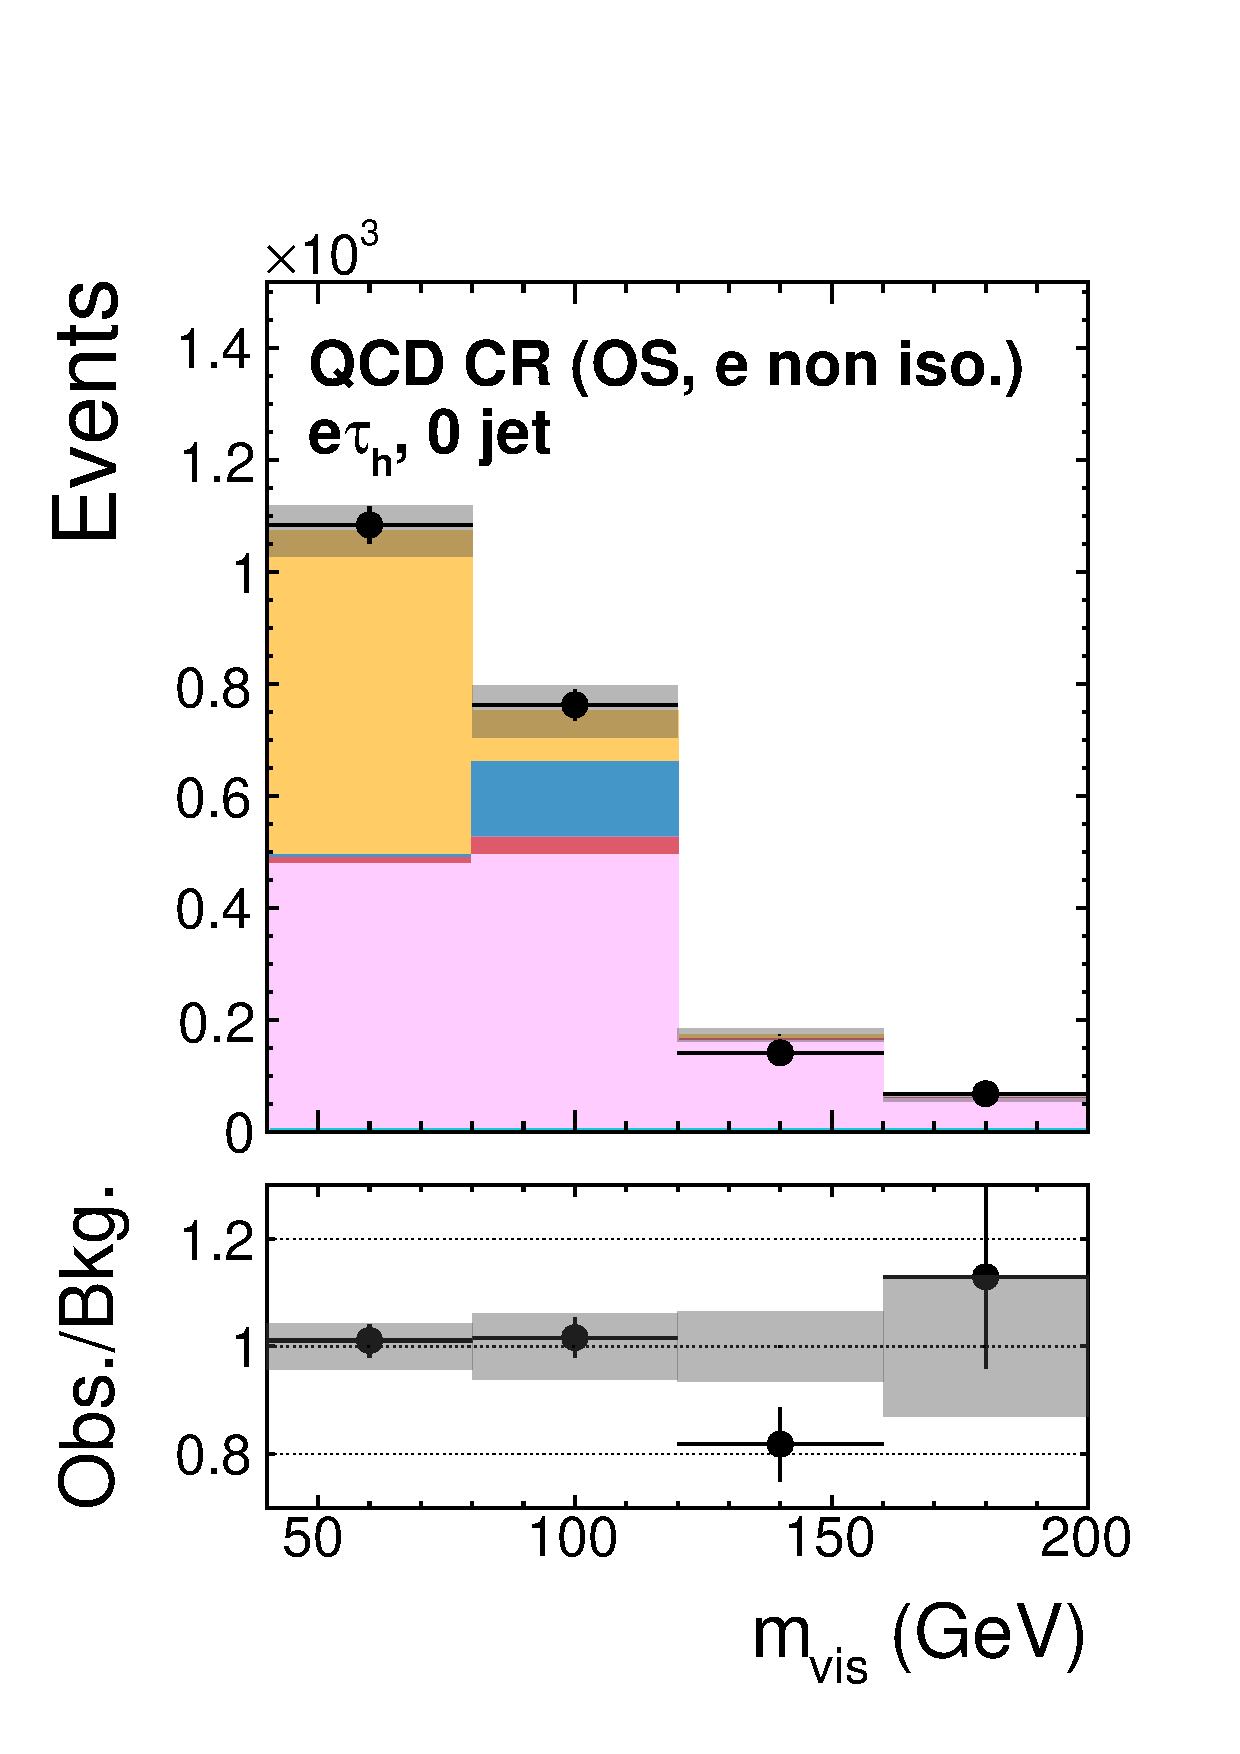
\includegraphics[width=0.3\textwidth]{higgs_to_taus/plots/Figure_003-d.pdf}
%     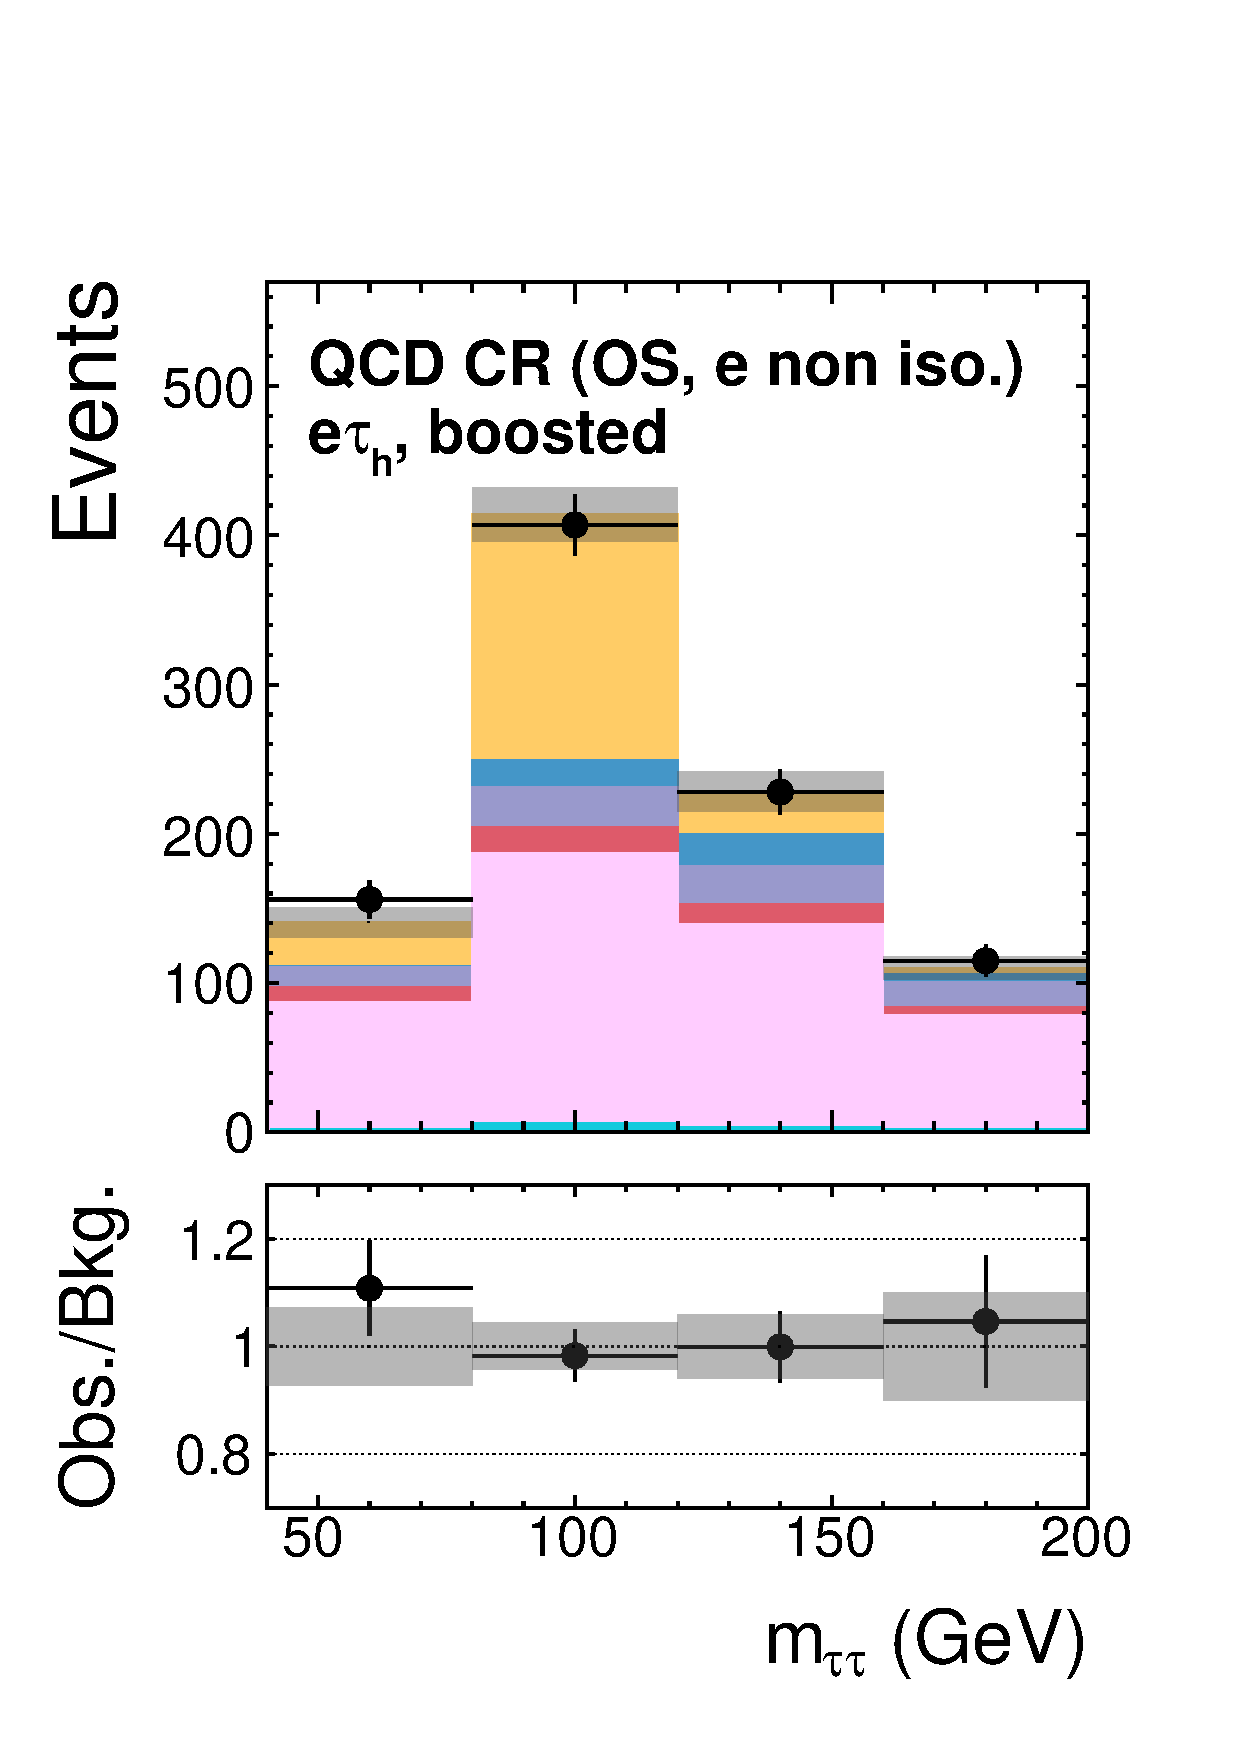
\includegraphics[width=0.3\textwidth]{higgs_to_taus/plots/Figure_003-e.pdf}
%     \caption{Control regions enriched in the QCD multijet background used in the maximum likelihood fit, together with the signal regions, to extract the results. The normalization of the predicted background distributions corresponds to the result of the global fit. These regions, defined by selecting events with opposite-sign $\ell$ and $\tauh$ candidates with $\ell$ passing inverted isolation conditions,  control the
%yields of the QCD multijet background in the $\Pgm\tauh$ and $\Pe\tauh$ channels.  The constraints obtained in the Boosted categories are propagated to the VBF categories of the corresponding channels.}
%     \label{fig:htt_qcd_CR3}
%\end{figure*}

In the $\tauh\tauh$ channel, the large QCD multijet background is estimated differently than
the other channels. Instead of deriving the QCD multijet shape template from the same-sign
region, the template is instead derived from the opposite-sign region using 
equation~\ref{eqn:qcd_eqn}. The reason for this is that the shape of the QCD multijet
distributions are difference between the same-sign and opposite-sign regions in the
$\tauh\tauh$ channel. The difference in these shape templates is statistically
evaluated using Kolmogorov-Smirnov (KS) tests. The KS test is a nonparametric test of the compatibility
of continuous, one-dimensional probability distributions. Specifically, this study relied
on a two sample, binned KS test which tested the compatibility of the QCD multijet
estimated background in the same-sign region with that estimated in the opposite-sign region.
The results of these compatibility tests are summarized in table~\ref{tab:htt_qcd_ks}.
Beyond showing the incompatibility of same-sign and opposite-sign shapes, different
isolation requirements were used to test the compatibility of QCD multijet shapes
across different isolation ranges for i) the same-sign events, and ii) again for the
opposite-sign events. These tests showed a much higher degree of shape compatibility
for events with different isolation requirements, but the same charge configuraion.
Because of this, a relaxed isolation criteria is used to derive the QCD multijet
template for the $\tauh\tauh$ channel.

\begin{table}[h!]
\begin{center}
{\footnotesize
\begin{tabular}{|c|c|c|}
\hline
Sign Configuration & $\tau_{h,2}$ Isolation Cuts & KS Test Value \\
\hline
%SS vs. OS & $\tau_{h,2}$!=VTight \&\& $\tau_{h,2}$==Tight & 0.033 \\
%SS vs. OS & $\tau_{h,2}$!=Tight \&\& $\tau_{h,2}$==Medium & 0.003 \\
%SS vs. OS & $\tau_{h,2}$!=Medium \&\& $\tau_{h,2}$==Loose & $<$0.001 \\
%SS vs. OS & $\tau_{h,2}$!=VTight \&\& $\tau_{h,2}$==Loose & 0.001 \\
SS vs. OS & Not VTight and Passes Tight & 0.033 \\
SS vs. OS & Not Tight and Passes Medium & 0.003 \\
SS vs. OS & Not Medium and Passes Loose & $<$0.001 \\
SS vs. OS & Not VTight and Passes Loose & 0.001 \\
\hline
\end{tabular}
\begin{tabular}{|c|c|c|c|}
\hline
Charge Config. & $\tau_{h,2}$ Iso. Cuts Shape 1 & $\tau_{h,2}$ Iso. Cuts Shape 2 & KS Test Value \\
\hline
%OS & $\tau_{h,2}$!=Tight \&\& $\tau_{h,2}$==Medium & $\tau_{h,2}$!=VTight \&\& $\tau_{h,2}$==Tight & 0.168 \\
%OS & $\tau_{h,2}$!=Medium \&\& $\tau_{h,2}$==Loose & $\tau_{h,2}$!=Tight \&\& $\tau_{h,2}$==Medium & 0.104 \\
%OS & $\tau_{h,2}$!=Medium \&\& $\tau_{h,2}$==Loose & $\tau_{h,2}$!=VTight \&\& $\tau_{h,2}$==Tight & 0.543 \\
OS & Not Tight and Passes Medium & Not VTight and Passes Tight & 0.168 \\
OS & Not Medium and Passes Loose & Not Tight and Passes Medium & 0.104 \\
OS & Not Medium and Passes Loose & Not VTight and Passes Tight & 0.543 \\
\hline
%SS & $\tau_{h,2}$!=Tight \&\& $\tau_{h,2}$==Medium & $\tau_{h,2}$!=VTight \&\& $\tau_{h,2}$==Tight & 0.587 \\
%SS & $\tau_{h,2}$!=Medium \&\& $\tau_{h,2}$==Loose & $\tau_{h,2}$!=Tight \&\& $\tau_{h,2}$==Medium & 0.036 \\
%SS & $\tau_{h,2}$!=Medium \&\& $\tau_{h,2}$==Loose & $\tau_{h,2}$!=VTight \&\& $\tau_{h,2}$==Tight & 0.029 \\
SS & Not Tight and Passes Medium & Not VTight and Passes Tight & 0.587 \\
SS & Not Medium and Passes Loose & Not Tight and Passes Medium & 0.036 \\
SS & Not Medium and Passes Loose & Not VTight and Passes Tight & 0.029 \\
\hline
\end{tabular}
}
\end{center}
\caption{
Kolmogrov-Smirnov test results comparing estimated QCD multijet shape templates to test shape compatibility
between different possible QCD multijet shape estimation regions. The $\tauh$ MVA isolation selection
for each comparison is listed where ``VTight'' means \texttt{Very Tight Tau MVA}, ``Tight'' means \texttt{Tight Tau MVA},
``Medium'' means \texttt{Medium Tau MVA}, and ``Loose'' means \texttt{Loose Tau MVA}.
In these comparisons the isolation of the highest $\pt$ $\tauh$, $\tau_{h,1}$,
is kept at \texttt{Medium Tau MVA} isolation.  
The upper table shows comparisons between same-sign (SS) and opposite-sign (OS) selections for the same
exact isolation selection. The lower table shows KS test results for comparisons
within the same charge configuration across different isolation requirements.
}
\label{tab:htt_qcd_ks}
\end{table} 

The selection used to estimate the QCD multijet background shape template and raw yield requires 
that at least one of the $\tauh$
must fail the \texttt{Tight Tau MVA} requirement which is the isolation selection used to 
define the signal region. This selection
ensures that the side-band sample is disjoin from the signal region.
In this region, the QCD multijet background shape and raw yield are obtained
by subtracting the contribution of the Drell--Yan, \ttbar, and $\PW+\text{jets}$ processes
from the data as in equation~\ref{eqn:qcd_eqn}.
A schematic representation of the $\tauh\tauh$ signal region and QCD multijet relaxed
isolation estimation region is in figure~\ref{fig:htt_tautau_qcd_schematic1}.


\begin{figure*}[htbp]
\centering
     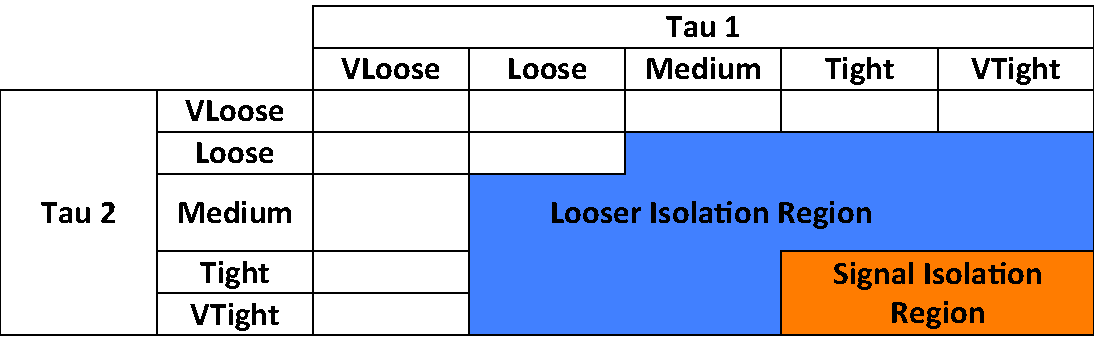
\includegraphics[width=0.6\textwidth]{higgs_to_taus/plots/tautau_QCD_signal_region.pdf}
     \caption{
Schematic depicting the range of $\tauh$ MVA working points ranging from very loose (\texttt{VLoose})
to very tight (\texttt{VTight}). The signal region is depicted in orange where both $\tauh$ meet the \texttt{Tight}
or \texttt{VTight} criteria. The QCD multijet relaxed isolation estimation region is depicted in blue and
does not overlap with the signal region.
     }
     \label{fig:htt_tautau_qcd_schematic1}
\end{figure*}

A scaling factor is required to adjust the raw yield estimated in the relaxed isolation region to the expected
QCD multijet yield in the signal extraction region. This extrapolation factor
is estimated in the same-sign charge region. Two same-sign QCD multijet samples are constructed
using 1) the exact same isolation requirements as the signal region; all selections are identical
here except for the $\tauh$ charge configuration. And, 2) a second region with the exact 
same relaxed isolation requirements as the region used to estimate the opposite-sign
QCD multijet shape template and raw yield. From these two samples a ``Relaxed-Region-to-Signal-Region''
scaling factor is calculated as,
\begin{equation}
\label{eqn:htt_tt_qcd_sf}
\text{Relaxed-Region-to-Signal-Region SF} = \frac{\text{SS Signal Region Yield}}{\text{SS Relaxed Region Yield}}
\end{equation}
where (SS) is same-sign.
Multiplying the raw yield estimated above by this scaling factor results in the estimated
QCD multijet contribution in the signal region. The ``Relaxed-Region-to-Signal-Region'' scale factors
for the three $\tauh\tauh$ categories are listed in table~\ref{tab:htt_qcd_sf}. The uncertainties associated
with these scale factors are propagated through the QCD multijet estimation process and combined
with results from closure tests to estimate a final category dependant systematic and statistic uncertainty
for the QCD multijet estimation process.

\begin{table*}[htbp]
\centering
\begin{tabular}{|l|c|}
\hline
Category   &   ``Relaxed-Region-to-Signal-Region''   \\
           &   Scale Factor   \\
\hline
0-jet      &    0.25 $\pm$ 1.0\%  \\
VBF        &    0.18 $\pm$ 9.8\%  \\
Boosted    &    0.23 $\pm$ 1.4\%  \\  
\hline
\end{tabular}
\label{tab:htt_qcd_sf}
\caption{
The category dependant scale factors used to adjust the QCD multijet yield to correspond 
to the expected yield in the signal region. The large uncertainty on the VBF scale factor shows the
limited amount of QCD multijet events in the VBF same-sign region. 
}
\end{table*}

The events selected with opposite-sign $\tauh$ candidates passing relaxed isolation requirements 
form control regions, shown in Fig.~\ref{fig:htt_qcd_CR4}, and are used in the global fit to extract the results.

\begin{figure*}[!htbp]
\centering
     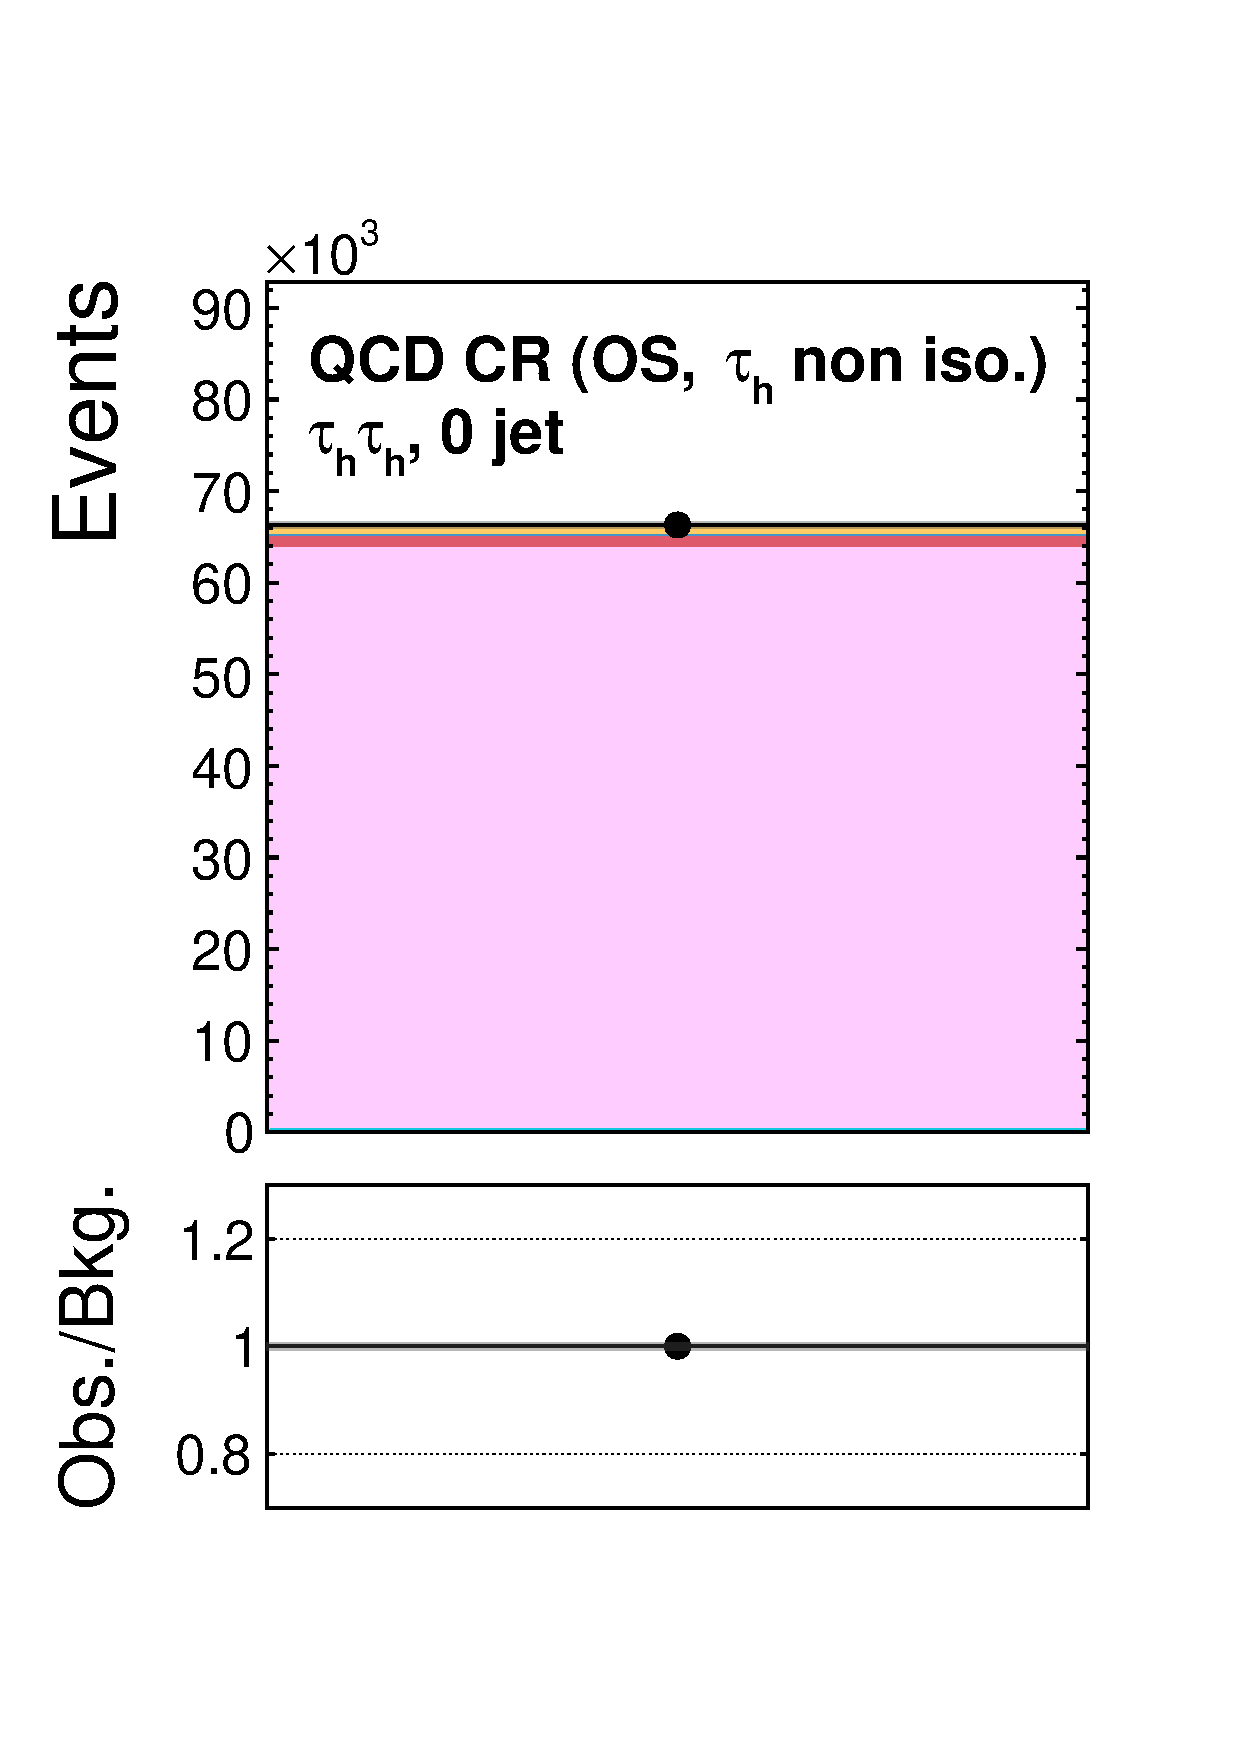
\includegraphics[width=0.24\textwidth]{higgs_to_taus/plots/Figure_004-a.pdf}
     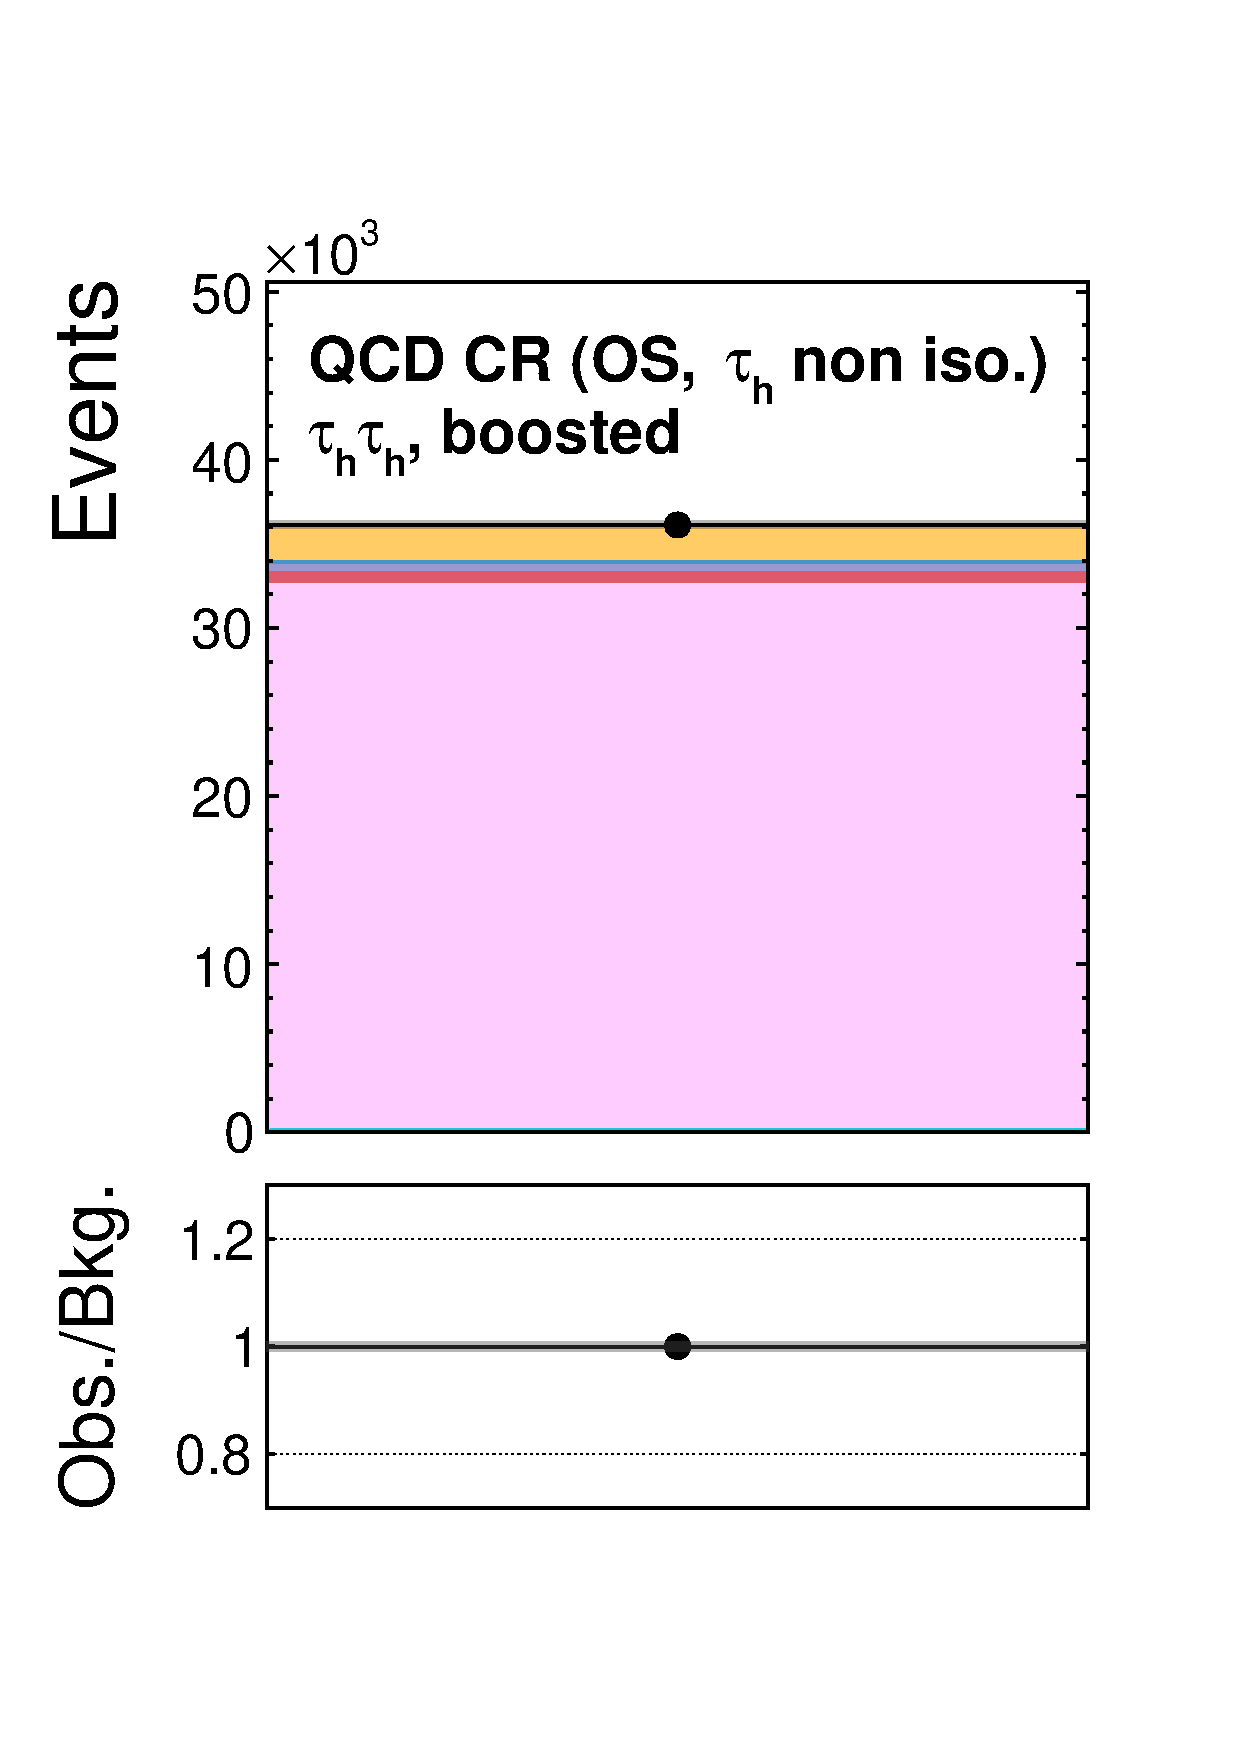
\includegraphics[width=0.24\textwidth]{higgs_to_taus/plots/Figure_004-b.pdf}
     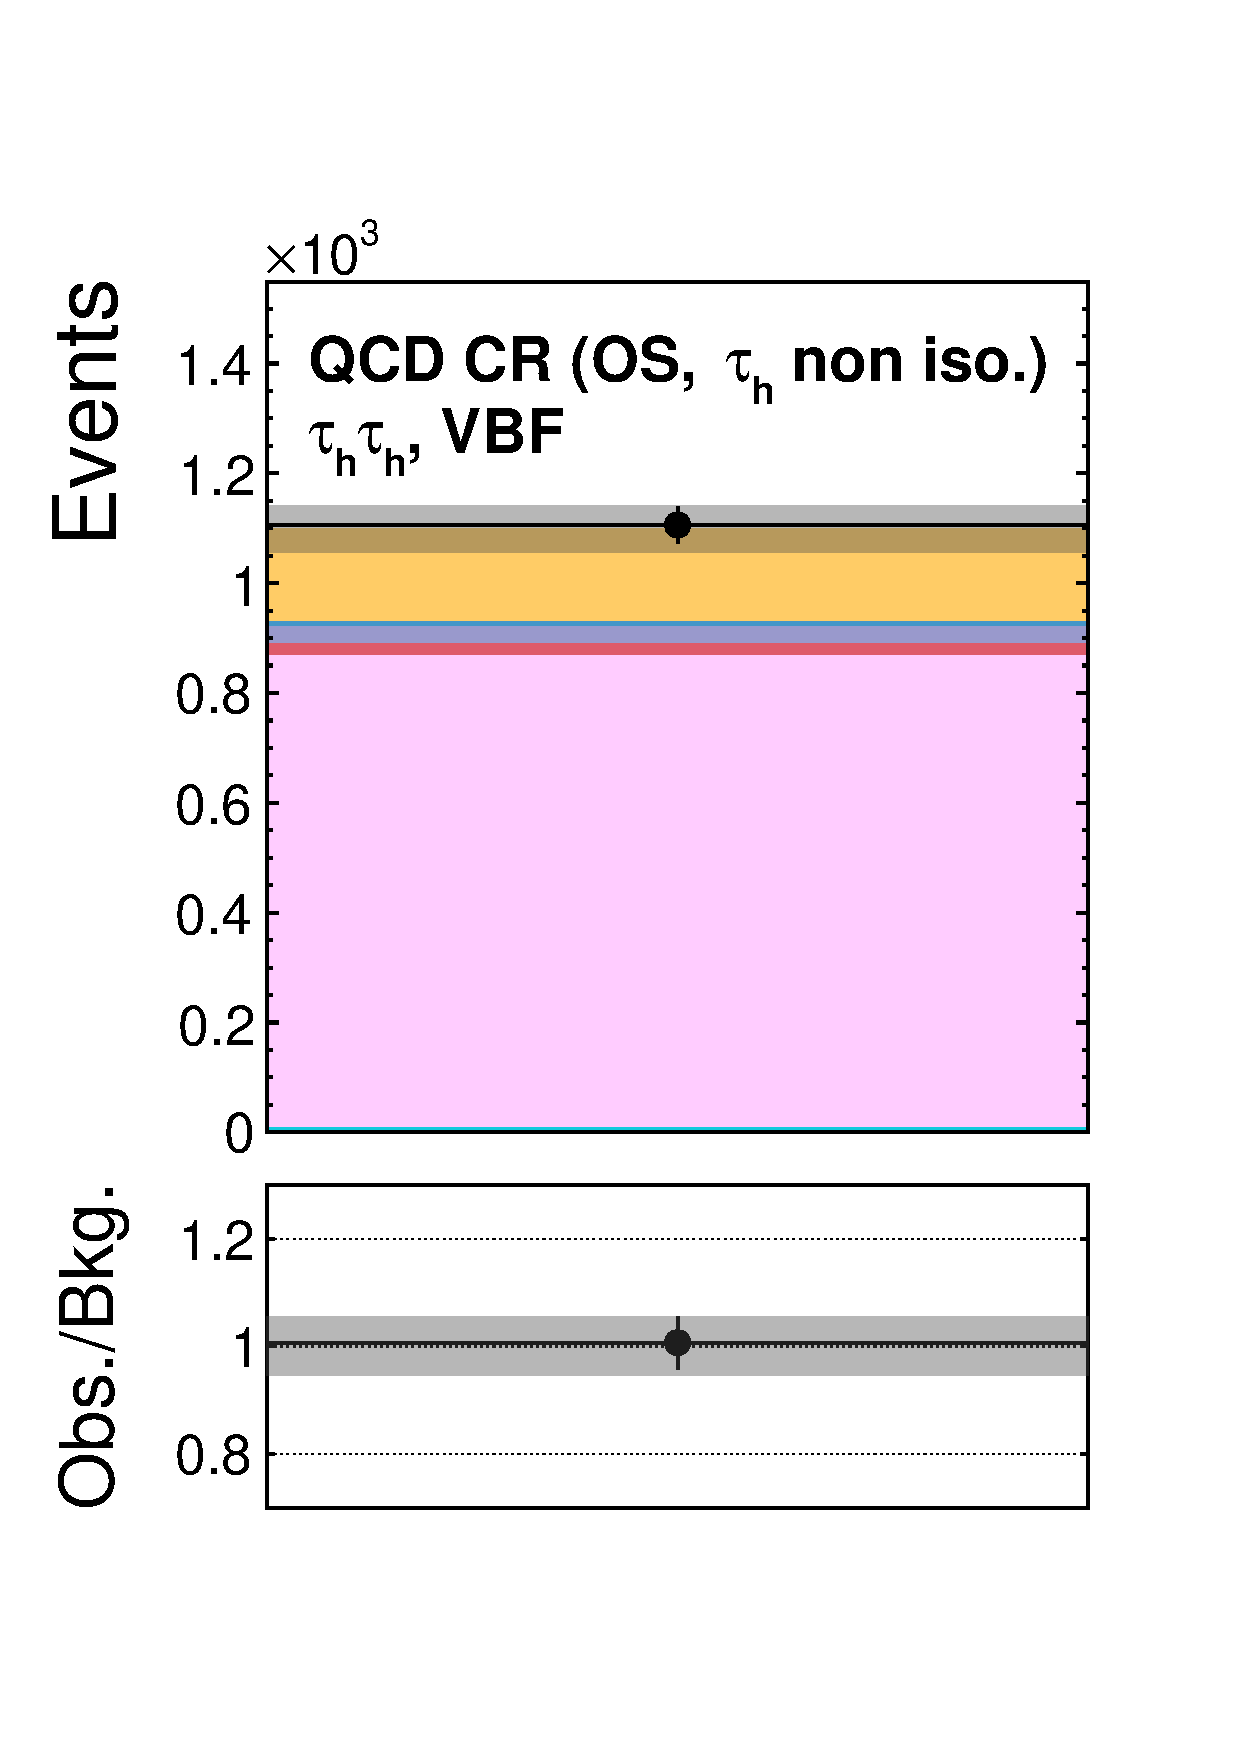
\includegraphics[width=0.24\textwidth]{higgs_to_taus/plots/Figure_004-c.pdf}
     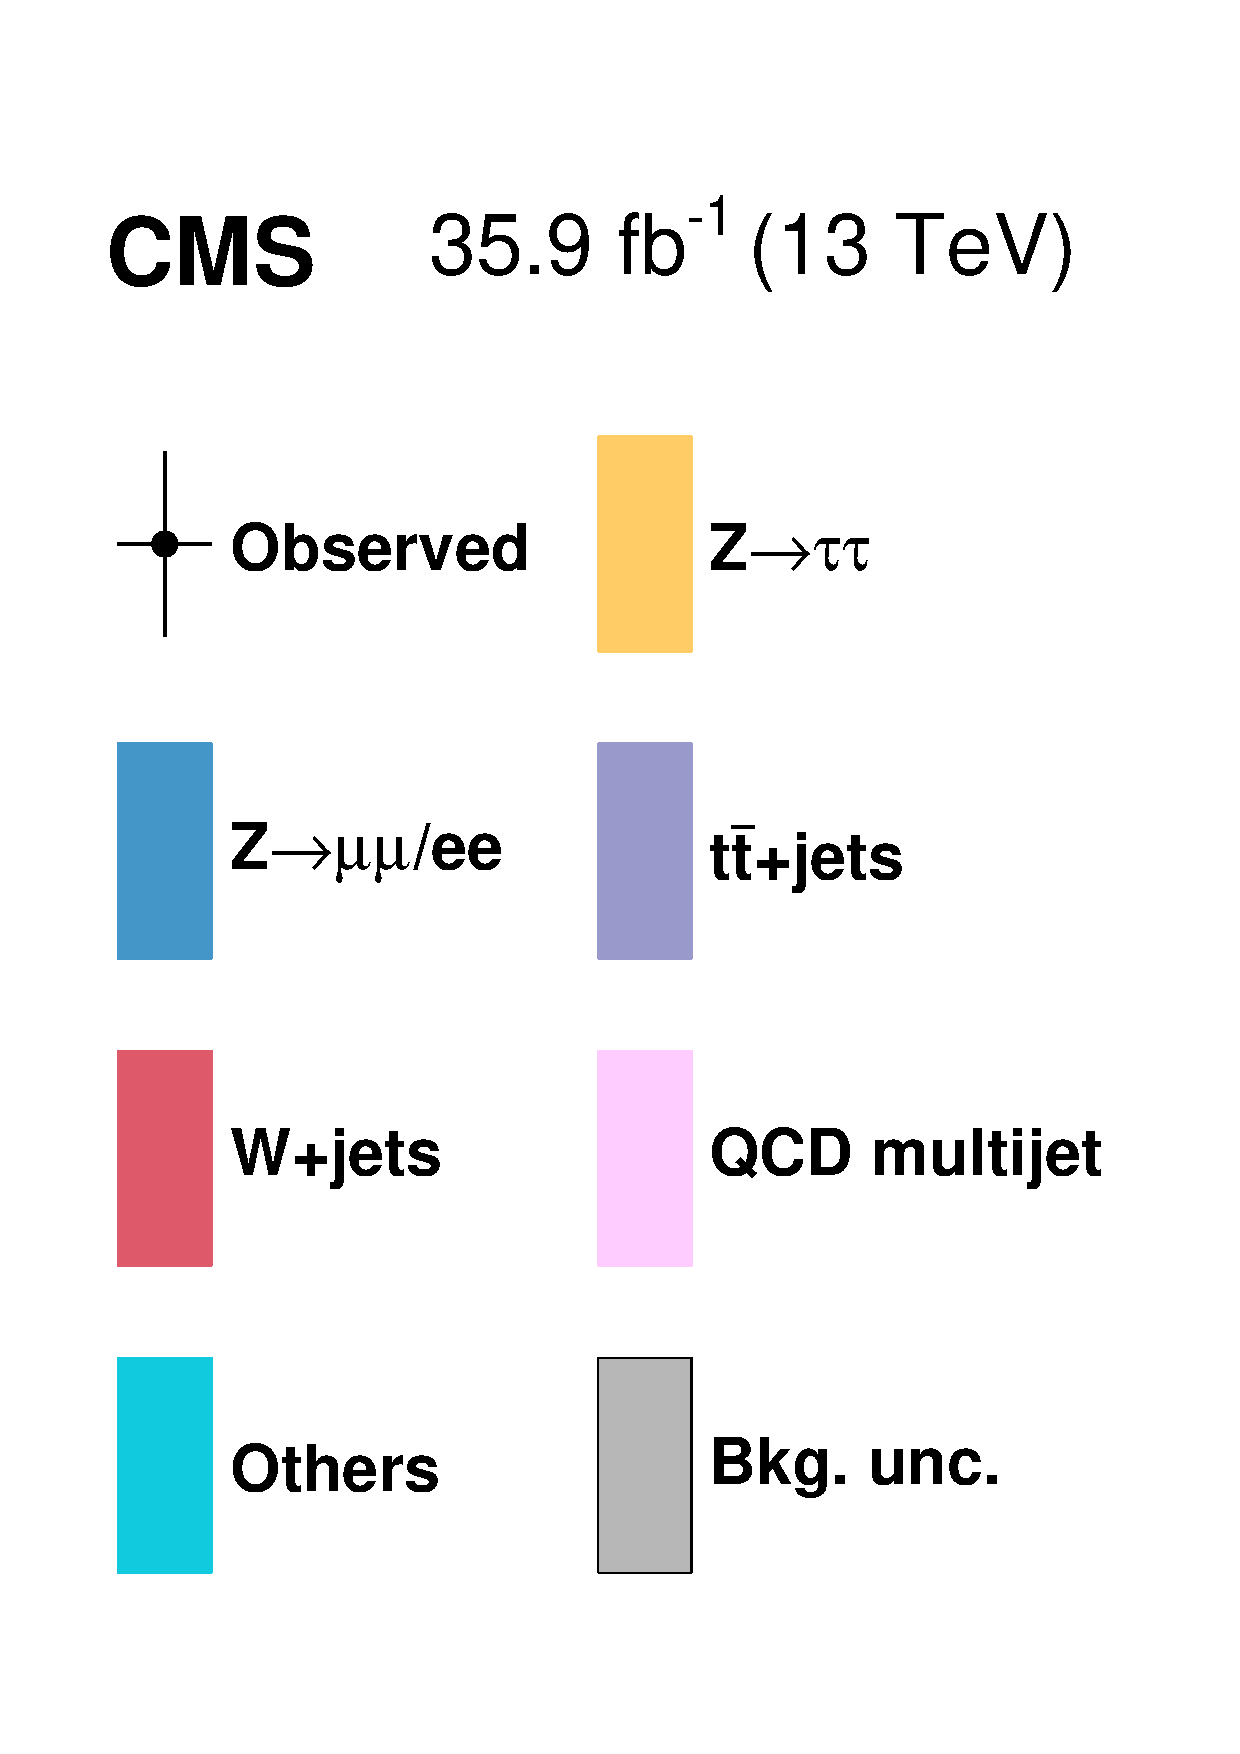
\includegraphics[width=0.24\textwidth]{higgs_to_taus/plots/Figure_004-d.pdf}
     \caption{Control regions enriched in the QCD multijet background used in the maximum likelihood fit, 
together with the signal regions, to extract the results. The normalization of the predicted background 
distributions corresponds to the result of the global fit. These regions, a formed by selecting events with 
opposite-sign $\tauh$ candidates passing relaxed isolation requirements with at least one of them
failing \texttt{Tight Tau MVA} isolation. These regions control the yields of the QCD multijet background 
in the $\tauh\tauh$ channel.}
     \label{fig:htt_qcd_CR4}
\end{figure*}


\subsubsection{\ttbar Background}
The \ttbar production process is one of the main backgrounds in the $\Pe\Pgm$ channel.
In all channels \ttbar is predicted from simulation. The normalization is adjusted using
a \ttbar-enriched control region orthogonal to the signal region. This control region is included
in the global fit. The control region is defined from the $\Pe\Pgm$ channel and the yield
of \ttbar in all channels and categories is adjusted by this singular \ttbar control region.
It is shown in figure~\ref{fig:htt_ttbar_CR2},
Orthagonality from the $\Pe\Pgm$ signal region is achieved by inverting the $p_\zeta$ requirement
and the events should contain at least one jet.

\begin{figure}[htb]
\centering
     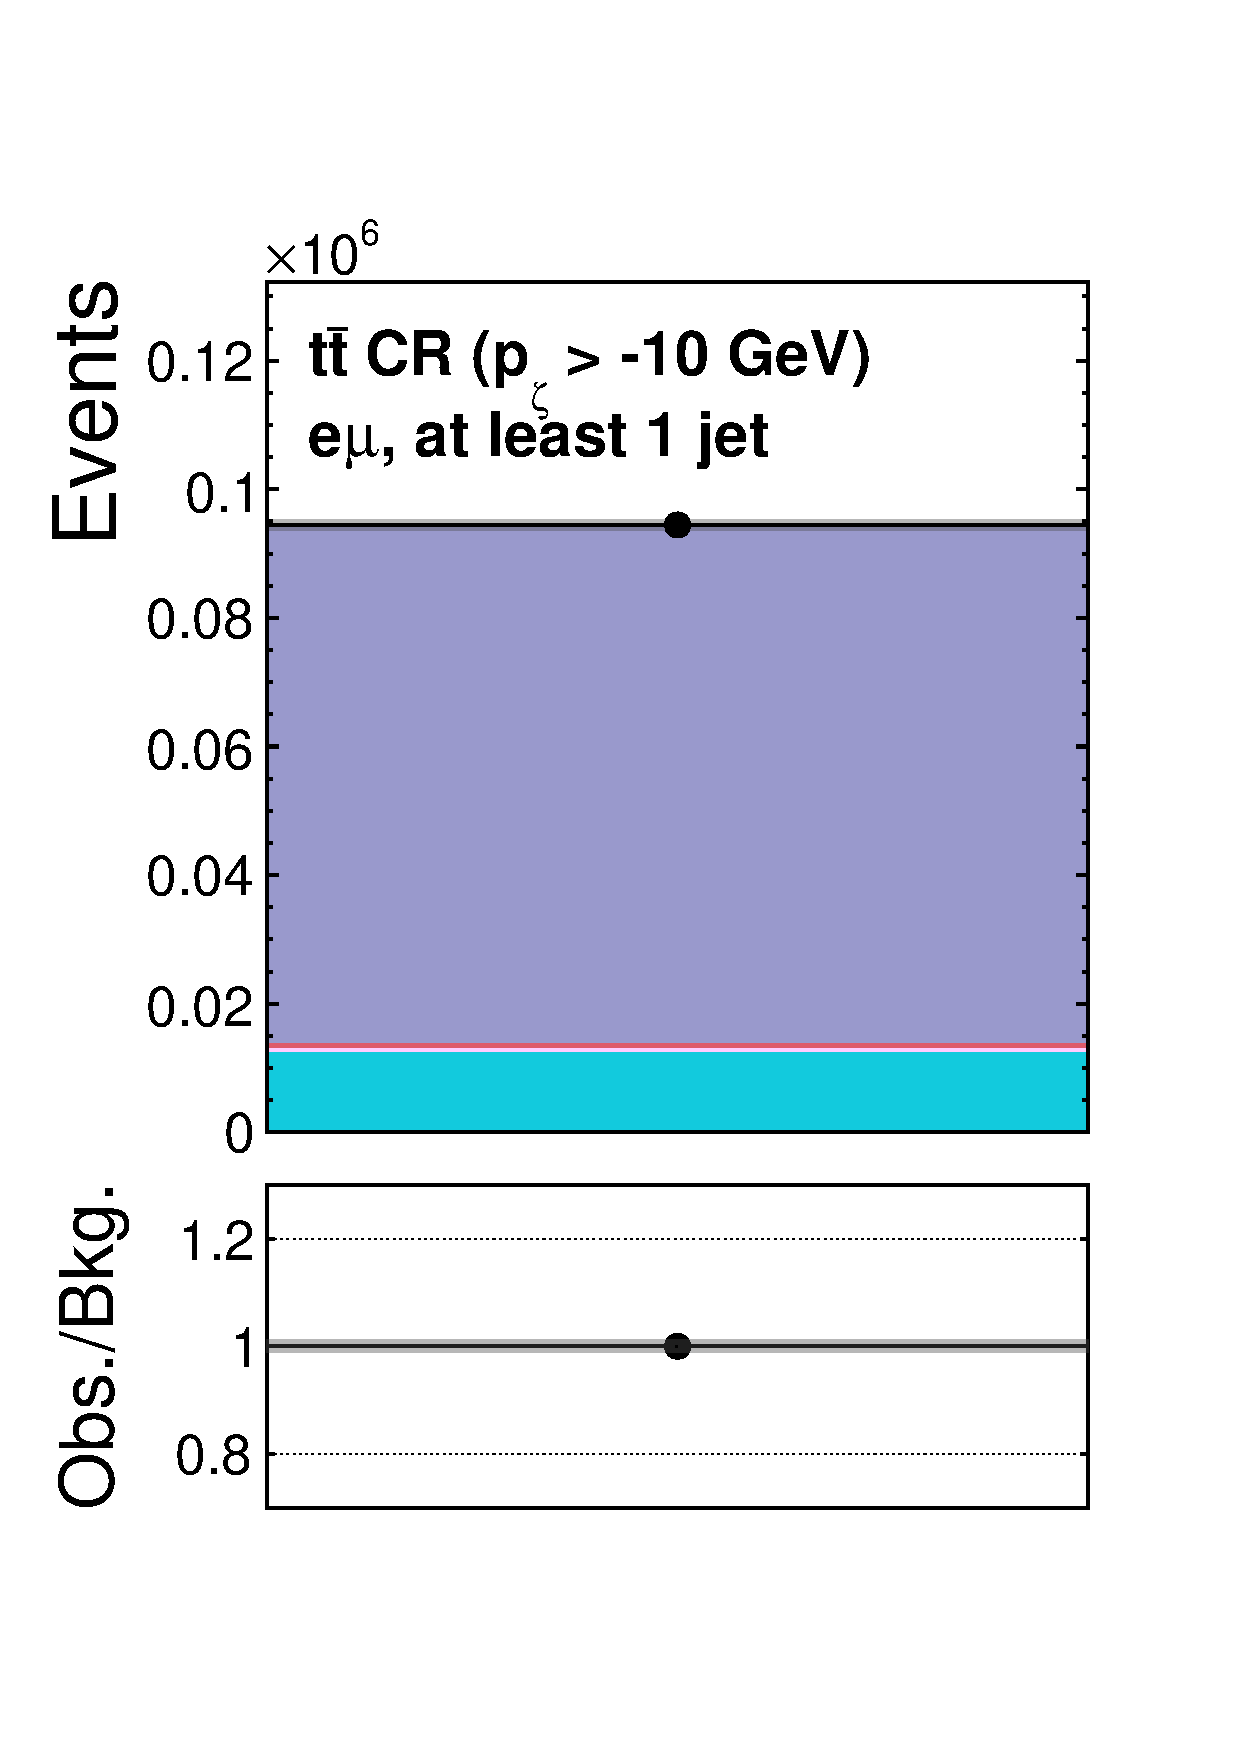
\includegraphics[width=0.23\textwidth]{higgs_to_taus/plots/Figure_005-a.pdf}
     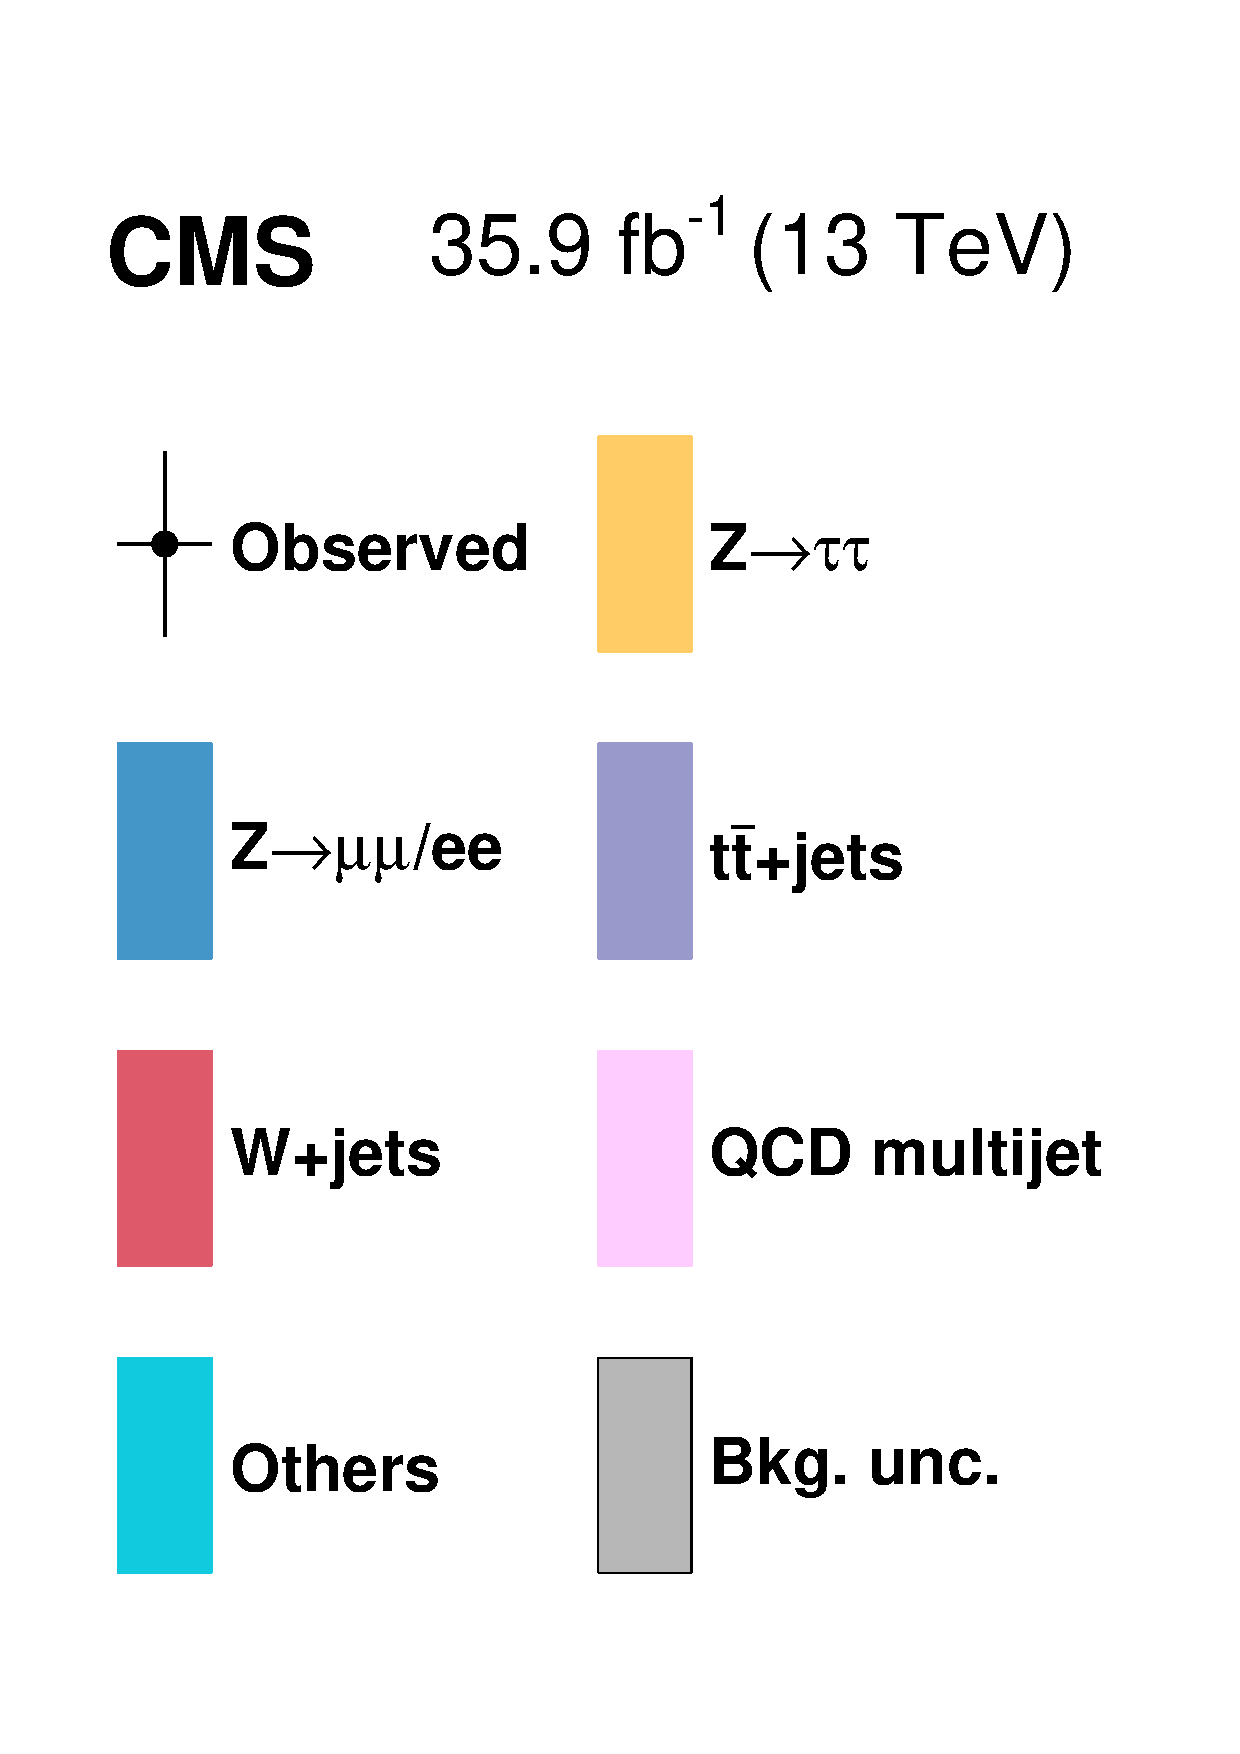
\includegraphics[width=0.23\textwidth]{higgs_to_taus/plots/Figure_005-b.pdf}
     \caption{Control region enriched in \ttbar background, used in the maximum likelihood fit, 
together with the signal regions, to extract the results. The normalization of the predicted background 
distributions corresponds to the result of the global fit. This region, defined by inverting the 
$p_\zeta$ requirement and rejecting events with no jet in the $\Pe\Pgm$ final state, is used to estimate the
yields of the \ttbar background in all channels.}
     \label{fig:htt_ttbar_CR2}
\end{figure}

Other background processes, such as, contributions from diboson and single top quark production, are estimated 
from simulation.


\section{Monte Carlo Corrections}
\label{sec:mc_corrections}

Corrections are applied to the simulated Monte Carlo samples to help correct for measured differences
between observed data and expectations based on simulation. Many of these corrections are designed
to correct differences in reconstruction and identification efficiencies for objects between data
and simulation. These corrections are derived in
fully orthogonal regions from the analysis signal regions when ever possible. There are however a
number of
instances where the $\Pgm\tauh$ channel is used to derive corrections. In these cases the measurement
region used to derive corrections will overlap with a subset of the analysis signal regions. This
overlap is discussed in the Systematic Uncertainties section~\ref{sec:htt_systematics}.


\subsection{Pileup Reweighting}
During 2016 data taking, the LHC delivered \pp collisions to CMS with an average of approximately 27
interactions per bunch crossing. Monte Carlo samples are generated with additional pileup interactions
added to the hard-scattering process for each event. A reweighting technique is used which improves
the aligment between the pileup interactions in data and those in simulation. This is critical because
there are some reconstructed event characteristics such as \etvecmiss which have different performance
in resolution and response depending on the number of pileup interactions in an event.


\subsection{Tau Identification Efficiency}
\label{sec:htt_tau_id_eff}
The reconstruction efficiency for hadronically decaying taus is observed to be different in data and in simulated samples.
Correction factors are derived by the Tau POG in the $\Pgm\tauh$ channel using a tag-and-probe method. Essentially,
the Tau ID Efficiency measurement selects $\PZ/\Pgg^*\to\Pgt\Pgt\to\Pgm\tauh$ events on the $\PZ$
mass peak and performs a fit with the $\PZ\to\Pgm\tauh$ process treated as a signal. The degree
to which the $\PZ\to\Pgm\tauh$ process is scaled up to down is the resulting Tau ID Efficiency
scale factor. The measured scale factor is 0.95 $\pm$ 5\% for all $\tauh$ passing \texttt{Tight Tau MVA}.
This correction factor is applied to all simulated $\tauh$ which are matched at the generator
level to $\tau$ leptons.


\subsection{Tau Energy Correction}
\label{sec:htt_tec}
The energy of each simulated $\tauh$, which matches to a $\tau$ at the generator level, is corrected
to better represent the observed energy of $\tauh$ in data. The correction is measured and applied
as a function of $\tauh$ decay mode with each correction listed in table~\ref{tab:htt_tec}. The measurement
of this correction is performed in the $\Pgm\tauh$ final state by the Tau POG. The effect of
the shifted $\tauh$ energy is fully propagated through to the \etvecmiss for each event.

\begin{table*}[htbp]
\centering
\begin{tabular}{|l|c|}
\hline
$\tauh$ Decay Mode   &   Energy Correction   \\
\hline
1-prong            &   -1.8\%  $\pm$ 1.2\%  \\
1-prong+$\PGpz$    &   +1.0\%  $\pm$ 1.2\%  \\
3-prong            &   +0.4\%  $\pm$ 1.2\%  \\  
\hline
\end{tabular}
\label{tab:htt_tec}
\caption{
Energy corrections applied to simulated genuine $\tauh$. The energy corrections are measured
and applied depending on the reconstructed decay mode of the $\tauh$.
}
\end{table*}



\subsection{Lepton Identification and Isolation Efficiencies}
Similar to the Tau ID Efficiency measured above, the electron and muon reconstruction, identification,
and isolation efficiencies are measured in both data and simulation. Correction factors equal to
$\epsilon_{data}/\epsilon_{MC}$ are derived as a function of both lepton $\pt$ and lepton $\eta$.
The electron (muon) efficiencies are measured in $\PZ\to\Pe\Pe$ ($\PZ\to\Pgm\Pgm$) events using a tag-and-probe
method.


\subsection{Trigger Efficiencies}
\label{sec:htt_trigger_eff}
Trigger efficiencies are measured in data and in simulation for all of the channels. For the channels
which trigger on $\tauh$, the $\Pgm\tauh$ and $\tauh\tauh$ channels, the $\tauh$ efficiency is measured
using tag-and-probe in the $\Pgm\tauh$ final state. The efficiencies for the $\tauh\tauh$ channel
are measured with dedicated muon+$\tauh$ monitoring triggers. The $\tauh$ trigger requirements
are identical between the monitoring trigger and the $\tauh\tauh$ trigger paths. The tag-and-probe
is conducted using the Single Muon PD. The selection for the $\tauh$ trigger efficiency measurements 
requires one well identified and isolated muon per event. The muon is required to fire a single muon trigger.
Events with at least one $\tauh$ which passes \texttt{decay mode finding} and \texttt{Tight Tau MVA} isolation
constitute the denominator selection for the efficiency measurement. Events where the $\tauh$
fires the trigger under study are recorded as passing events. The ratio of passing events to
denominator events defines the trigger efficiency. Trigger efficiencies are measured and applied as 
a function of $\tauh$: $\pt$, decay mode, and generator matching status. Figure~\ref{fig:htt_tt_trig}
shows the trigger efficiency versus $\pt$ for the double-$\tauh$ trigger.

\begin{figure*}[!htbp]
\centering
     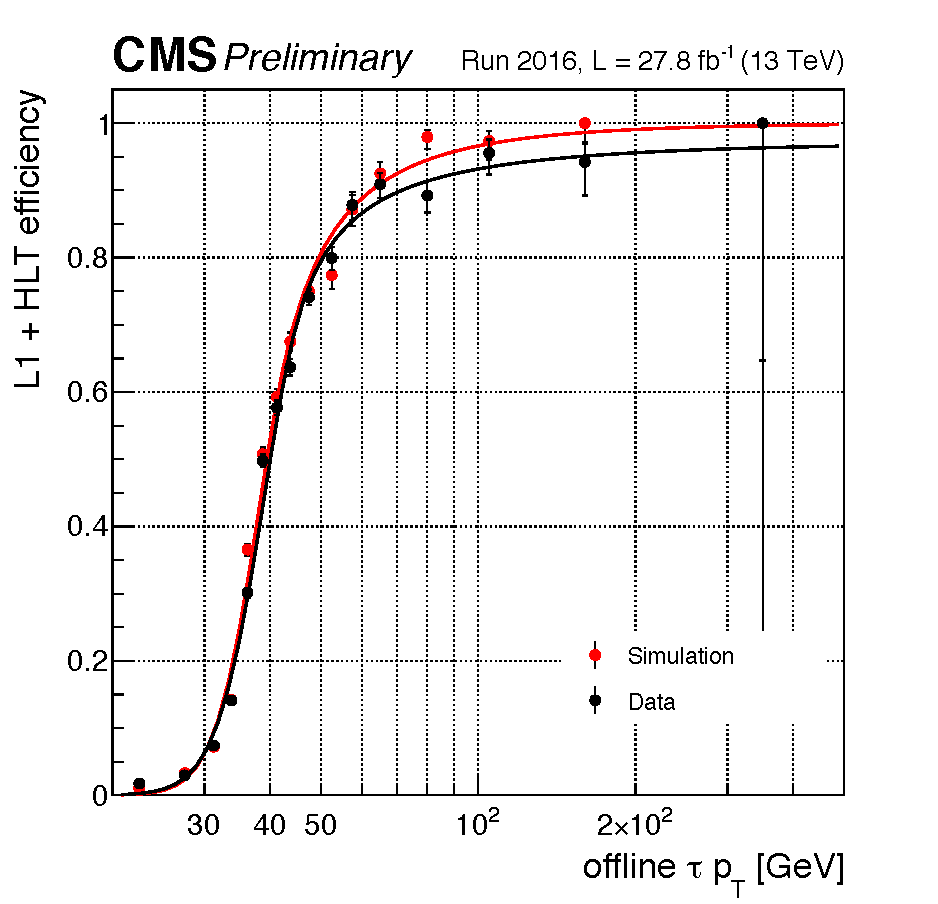
\includegraphics[width=0.65\textwidth]{higgs_to_taus/plots/htt_tautau_trigger_efficiency.pdf}
     \caption{
Comparison of the trigger efficiencies for the \texttt{HLT\_DoubleMediumIsoPFTau35\_Trk1\_eta2p1\_Reg}
which was active in data during eras B-G. The efficiency was measured using tag-and-probe in the
$\Pgm\tauh$ final state. The efficiency is measured for a single leg of the double-$\tauh$
with a muon+$\tauh$ monitoring trigger. The efficiencies shown here are used in the $\tauh\tauh$ channel.
The specific distribution shown is for genuine $\tau$ leptons and includes all used decay modes.
}
     \label{fig:htt_tt_trig}
\end{figure*}

The trigger efficiencies for electrons and muons are also measured with a tag-and-probe method.
Similar to the electron and muon identification and isolation efficiencies, the 
electron (muon) trigger efficiencies are measured in $\PZ\to\Pe\Pe$ ($\PZ\to\Pgm\Pgm$) events.
The denominator selection for the probe lepton requires the same identification and
isolation criteria used in the analysis. The efficiencies are measured as a function of
lepton $\pt$ and $\eta$.



\subsection{Drell--Yan Reweighting}
\label{sec:htt_dy_reweighting}
The simulated Monte Carlo Drell--Yan sample used in the analysis is simulated at leading order (LO)
using the \MGAMCNLO generator discussed in section~\ref{sec:simulation}. To assess Monte Carlo to
data agreement a dedicated $\PZ/\Pgg^*\to\Pgm\Pgm$ control region with high Drell--Yan purity was used.
The $\PZ/\Pgg^*\to\Pgm\Pgm$ control region selected events from the Single Muon PD and requires the 
presence of two well-identified muons with $\pt > 25 \GeV$ and an invariant mass between 70 and 110\GeV.
With this selection criteria over 99\% of the events are attributed to $\PZ/\Pgg^*\to\Pgm\Pgm$ decays.

Differences in the distributions of $m_{\ell\ell}$ and $\pt^{\ell\ell}$ between data and 
in simulations are observed in this control region. To correct for this, 2D weights based on these variables 
are derived and applied to simulated $\PZ/\Pgg^*\to\Pgt\Pgt, \ell\ell$ events in the signal region of the analysis. 
In addition, corrections depending on $\mjj$ are derived from the $\PZ/\Pgg^*\to\Pgm\Pgm$ region and 
applied to the $\PZ/\Pgg^*\to\Pgt\Pgt, \ell\ell$ simulation for events with at least two jets passing the 
VBF category selection criteria. After this reweighting, good agreement between data in the 
$\PZ/\Pgg^*\to\Pgm\Pgm$ region and simulation is found for all other variables used in the analysis.
These derived corrections are also applied to the simulated samples of electroweak production of $\PZ$ 
bosons. Electroweak produced $\PZ$ bosons contribute up to 8\% of the $\PZ$ boson production in the VBF category.



\subsection{Hadronic Recoil Corrections}
Recoil corrections are applied to the Drell--Yan and $\PW+\text{jets}$ simulated background events 
as well as the simulated signal events for 
Higgs bosons produced via the gluon fusion or VBF mechanisms. Recoil corrections correct for the
mismodeling of \etvecmiss in the simulated samples. A variable, $\vec{U}$, is defined as the 
vectorial difference of the measured \etvecmiss and the total transverse momentum of neurtrinos
originating from the decay of the boson.
\begin{equation}
\vec{U} = \etvecmiss - \vec{p}_{\text{T},\nu}
\end{equation}

For $\PZ$ bosons decaying leptonically to $\ell$, $\vec{U}$ can be expressed as,

\begin{equation}
\vec{U} = \vec{p}_{\text{T,B}} - \vec{H}_{\text{T}}
\end{equation}

where $\vec{H}_{\text{T}}$ is the transverse momentum of hadronic recoil and $\vec{p}_{\text{T,B}}$
is the leptonic recoil and is the transverse momentum of leptonically decaying $\PZ$, $\PW$, or Higgs bosons.

Like the Drell--Yan Reweighting mentioned above, $\vec{U}$ is measured in $\PZ\to\Pgm\Pgm$ events.
It is observed that the $\vec{H}_{\text{T}}$ from simulation in $\PZ\to\Pgm\Pgm$ does not align with
the $\vec{H}_{\text{T}}$ from data. A reweighting method is derived to align the simulated distribution with 
data. The $\PZ/\Pgg^*\to\Pgm\Pgm$
final state is used because of the absence of neutrinos in the $\PZ$ decay making the comparison of
the simulation to data and derivation of the reweighting technique far more simple. For the measurement
and application of the corrections $\vec{U}$ is decomposed into two components, one which is
paralled to $\vec{p}_{\text{T,B}}$ ($\vec{U_{1}}$) and one which is orthogonal ($\vec{U_{2}}$).


\subsection{Generator Event Weights}
Generator weights are applied on a per event basis. Samples produced with the \MGAMCNLO generator
contain both positive and negative event weights, as discussed in the Simulation chapter~\ref{sec:simulation}.
Negative generator weights in a sample reduces the effective statists of that sample. This reduction
in statistical power is often the trade off for increased precision in the modeling of a choosen
background or signal process.


\subsection{Luminosity Weighting}
The event weights for simulated events are scaled to the expected yields for each sample. A per-event
weight (W) is defined based on the number of generated events (N), the best theory predicted cross section
for the process ($\sigma$), and the integrated luminosity of the dataset being modeled 
($\mathcal{L}$), 35.9\fbinv.

\begin{equation}
\text{W} \, = \mathcal{L} \, \,  \frac{\sigma}{\text{N}}
\end{equation}

For samples with negative generator weights, N is redefined as the sum total of the event weights to
properly account for the negative event weights.




\section{Systematic Uncertainties}
\label{sec:htt_systematics}

The systematic uncertainty model for the $\htt$ study was critical to the success of the analysis.
The goal of the analysis was to reach an observed significane for the Higgs boson of 5.0$\sigma$.
To achieve this the description of the expected background processes and Higgs boson signal
needed to be as close to data as possible. The previous Monte Carlo Reweighting 
section~\ref{sec:mc_corrections} detailed this process. Many of the corrections and weights applied
to the simulated samples have associated unceratinties which must be represented in the
global fit. Other unceratinties come from the measurement of the data itself such as the uncertainty
on the integrated luminosity. In addition to these, there are also theoretical uncertainties on
aspects such as the production cross sections for the simulated backgrounds and Higgs boson signals. 
These are all detailed in the sections below.


\subsection{Integrated Luminosity Uncertainties}
The total data taken by the CMS experiment in 2016 that is marked usable for physics is 35.9\fbinv. The uncertainty
on this 35.9\fbinv integrated luminosity value amounts to 2.5\%~\cite{CMS-PAS-LUM-17-001}.


\subsection{Object Reconstruction, Identification and Trigger Uncertainties}
The total uncertainty in the $\tauh$ identification efficiency measurement for genuine $\tauh$ leptons is 
5\% mentioned in Section~\ref{sec:htt_tau_id_eff}.
The $\tauh$ are required to pass different identification criteria per channel
specifically aimed at reducing the chance of fake $\tauh$ originating from different background
processes in each final state. Because of the different anti-$\Pe$ and anti-$\Pgm$ discriminators
applied in each channel, the 5\% uncertainty is not fully correlated among all the di-$\Pgt$ channels.

The trigger efficiency uncertainty per $\tauh$ candidate amounts to 5\%. This leads to a total 
trigger uncertainty of 10\% for processes estimated from simulation in the $\tauh\tauh$ decay channel. 
This uncertainty is based off of the tag-and-probe trigger efficiency measurement in 
$\PZ\to\Pgt\Pgt$ events detailed in section~\ref{sec:htt_trigger_eff}.

In the decay channels with muons or electrons, the uncertainties for the muon and electron identification, 
isolation, and trigger efficiencies lead to a total rate uncertainty of 2\% for muons and 2\% for electrons.


\subsection{Tau Fake Rate}
For events where muons or electrons are misidentified as $\tauh$ candidates, the $\tauh$ identification leads 
to rate uncertainties of 25\% and 12\%, respectively, per reconstructed $\tauh$ decay mode. These fake $\tauh$
dominantly come from $\PZ\to\Pgm\Pgm$ events in the $\Pgm\tauh$ decay channel and $\PZ\to\Pe\Pe$ events 
in the $\Pe\tauh$ decay channel. Using $\mvis$ and the reconstructed 
$\tauh$ decay mode as the observables in the 0-jet category of the $\Pgm\tauh$ and $\Pe\tauh$ channels helps constrain these 
uncertainties during the signal extraction fit. The post-fit uncertainty in the rate of muons or electrons 
misidentified as $\tauh$ per decay mode becomes of the order of 5\%. This is an 80\% constraint for the muon
misidentified as $\tauh$ rate and a 40\% constraint on the electron misidentified as $\tauh$ rate.


\subsection{Energy Scales}
\subsubsection{Visible Tau Energy Scale}
An uncertainty of 1.2\% in the visible energy scale of genuine $\tauh$ leptons affects both the shape of the
signal and background distributions and the expected yields. The 1.2\% uncertainty is treated as uncorrelated 
among the different $\tauh$ decay modes: 1-prong, 1-prong+$\PGpz$, and 3-prong.
The magnitude of the uncertainty was determined based on the uncertainties on the measured $\tauh$ energy 
corrections in Section~\ref{sec:htt_tec}. The measurement was conducted in the $\Pgm\tauh$ final state and
does have some overlap with the $\Pgm\tauh$ channel signal regions. However, the event overlap is found to be
less than 50\% between the $\tauh$ energy correction/visible $\tauh$ energy scale measurement region and the
$\Pgm\tauh$ signal region used in this analysis.

The fit constrains the visible $\tauh$ energy scale uncertainty to about 0.3\%, a 75\% constraint, for all 
decay modes. The constraint mostly comes from highly populated regions with high $\tauh$ purity, for example,
the 0-jet and Boosted categories of the $\Pgm\tauh$ and $\tauh\tauh$ channels. The constraint on the size of the 
uncertainty is explained by the addition of two other decay channels
with $\tauh$ candidates ($\tauh\tauh$ and $\Pe\tauh$) in addition to to the $\Pgm\tauh$ measurement region.
Additionally, the higher number of events in the Monte Carlo simulations and the finer categorization which 
leads to regions with a high $\PZ\to\Pgt\Pgt$ event purity also contribute to the post-fit constraint on the
visible tau energy scale.
Even in the most Boosted analysis categories, reconstructed $\tauh$ candidates typically have moderate 
$\pt$ (less than 100\GeV) and are
found in the barrel region of the detector. Tracks are well measured in the CMS detector in this $\pt$ range.
Therefore, the visible energy scale of genuine $\tauh$ leptons is fully correlated for all $\tauh$ leptons 
reconstructed in the same decay mode, irrespective of their $\pt$ and $\eta$. The uncertainties in the 
visible energy scale for genuine $\tauh$ leptons together contribute an uncertainty of 5\% to the measurement 
of the signal strength.


\subsubsection{Energy Scale for Fake Taus}
The energy scale uncertainty for muons or electrons
misidentified as $\tauh$ candidates is 1.5 or 3\%, respectively. It is uncorrelated between reconstructed $\tauh$ decay
modes. The fit constrains these uncertainties to about one third of their initial values. For events where quark- or 
gluon-initiated jets are misidentified as $\tauh$ candidates, a linear uncertainty that increases by 20\% per 100\GeV 
in $\tauh$ $\pt$ accounts for a potential mismodeling of the jet$\to\tauh$ misidentification rate as a
function of the $\tauh$ $\pt$ in simulations. The uncertainty has been determined from a region enriched in $\PW+\text{jets}$ 
events, using events in the $\Pgm\tauh$ final state, characterized by a large transverse mass 
between the $\etvecmiss$ and the muon~\cite{Khachatryan:2015dfa,CMS-PAS-TAU-16-002}.

\subsubsection{Jet Energy Scale}
The uncertainties in the jet energy scale depend on the $\pt$ and $\eta$ of the jet~\cite{CMS-JME-10-011}.
They are factorized into 27 distinct uncorrelated contributions. These factorized uncertainties target jet related 
mismodeling for different CMS subdetectors, namely ECAL and HCAL, uncertainties in jet energy corrections, timing dependance,
high $\pt$ jet extrapolations uncertainties, and large $\abs\eta$ jet related uncertainties. The uncertainties
affect the $\pt$ of each jet in an event. As the $\pt$ for each jet increasing or decreasing, the 
the number of jets with passing $\pt > 30\GeV$ is recomputed as is the $\mjj$ for each event. The adjusted number of
jets and $\mjj$ are used to determine the new, shifted, event categorization. For example,
events can shift between the 0-jet and Boosted category if a jet has a $\pt$ value near 30\GeV that shifts into
or out of categorization as a jet by the analysis (jet $\pt > 30\GeV$). As $\mjj$ is shifted, the shifted $\mjj$ value is used
to plot the event in the 2D VBF distribution.


\subsubsection{MET Energy Scale}
The \etvecmiss scale uncertainties~\cite{CMS-JME-12-002} are computed event-by-event and affect the normalization of 
various processes through the event selection in the $\ell\tauh$ channels which employ the low-\MT,
$\MT < 50\GeV$ criteria. The \etvecmiss scale uncertainties also affect event distributions through the 
propagation of these uncertainties 
to the di-$\Pgt$ mass $\mtt$. The \etvecmiss scale uncertainties which have the largest impact on the signal significance
in this analysis are from jet related uncertainties and unclustered energy deposits in the detector.
The unclustered energy deposites come from four independent sources related to the tracker, ECAL, HCAL, and 
forward calorimeter subdetectors. The jet related \etvecmiss scale uncertainties arise from uncertainties
in the jet energy scale measurement. As the scale of the jet energy is varied, these changes are propagated to
the \etvecmiss. The combination of both sources of uncertainties in 
the \etvecmiss scale leads to an uncertainty of about 10\% in the measured signal strength.


\subsubsection{Electron And Muon Energy Scale}
The uncertainty in the electron energy scale is 2.5\% in the endcaps and 1\% in the barrel of the detector. 
It is only relevant in the $\Pe\Pgm$ decay channel, where it affects the final distributions shape and yield.
In all channels, the effect of the uncertainty in the muon energy scale is negligible and is not included
in the systematic model.


\subsection{b-Tagging Uncertainties}
The $\htt$ analysis only applies a b-tagged jet selection criteria in the $\Pe\Pgm$ channel where the number
of b-tagged jets must equal zero in the signal region. The rate uncertainty related to discarding events 
with a b-tagged jet in the $\Pe\Pgm$ channel is up to 5\% for the $\ttbar$ background. The uncertainty 
in the mistagging rate of gluon and light-flavor jets is negligible.


%In the 0-jet category of the $\Pgm\tauh$ and $\Pe\tauh$ channels, the relative contribution of $\tauh$ in a given
%reconstructed decay mode is allowed to fluctuate by 3\% to account for the possibility that the reconstruction and
%identification efficiencies are different for each decay mode. This uncertainty has been measured in a region enriched 
%in $\PZ\to\Pgt\Pgt$ events with one $\Pgt$ lepton decaying hadronically and the other one decaying to a muon, by 
%comparing the level of agreement in exclusive bins of the reconstructed $\tauh$ decay mode, after adjusting the inclusive 
%normalization of the $\PZ\to\Pgt\Pgt$ simulation to its best-fit value. The effect of migration between the reconstructed 
%$\tauh$ decay modes is negligible in other categories, where
%all decay modes are treated together.


\subsection{Background Estimation Uncertainties}
\subsubsection{Drell--Yan Uncertainties}
The $\PZ\to\Pgt\Pgt$ background yield and distribution are corrected based on the agreement between data and the 
background prediction in a control region enriched in the $\PZ\to\Pgm\Pgm$ events, as explained in 
Section~\ref{sec:htt_dy_reweighting}. The extrapolation uncertainty related to kinematic differences between the selections 
in the signal and control regions ranges between 3 and 10\%, depending
on the category. Shape uncertainties related to the uncertainties in the applied corrections are considered.
They reach 20\% for some ranges of $\mjj$ in the VBF category, but are more modest in the $\tauh\tauh$ channel where
the uncertainties range from 0\% in the lowest $\mjj$ region to 6\% in the $500\GeV < \mjj < 800\GeV$ region.
These uncertainties arise from the different level of agreement between data and simulation in the 
$\PZ\to\Pgm\Pgm$ control region obtained when varying the threshold on the muon $\pt$.


\subsubsection{$\PW+\text{jets}$ Uncertainties}
The uncertainties in the $\PW+\text{jets}$ event yield for the $\Pgm\tauh$ and $\Pe\tauh$ channels are determined 
from their $\PW+\text{jets}$ control regions. The uncertainties account for the statistical uncertainties of the
data and $\PW+\text{jets}$ simulated samples. An extrapolation uncertainty is also determined which accounts for
the high-\MT ($\MT>80\GeV$) control regions to the low-\MT ($\MT<50\GeV$) signal regions scaling.
These uncertainties ranges from 5 to 10\%.
% and is obtained by comparing the \MT distributions of simulated and observed 
%$\PZ\to\Pgm\Pgm$ events where one of the muons is removed and the \etvecmiss adjusted accordingly, to mimic 
%$\PW+\text{jets}$ events. The reconstructed invariant mass of the parent boson in the rest frame is multiplied by the 
%ratio of the $\PW$ and $\PZ$ boson masses before removing the muon.

In the $\tauh\tauh$ and $\Pe\Pgm$ channels, where the $\PW+\text{jets}$ background is estimated from simulation, the 
uncertainty on the yield of this small background is 4\% and 20\%, respectively. The larger value for the 
$\Pe\Pgm$ channel includes uncertainties in the misidentification rates of jets as electrons and muons, whereas the 
uncertainty in the misidentification rate of jets as $\tauh$ candidates in the $\tauh\tauh$ channel is accounted for 
by the linear uncertainty as a function of the $\tauh$ $\pt$ described earlier.


\subsubsection{QCD Multijet Uncertainties}
The uncertainty in the QCD multijet background yield in the $\ell\tauh$ and $\Pe\Pgm$ channels ranges from 10 to 20\%.
They are category dependant and account for the uncertainty on the extrapolation from the same-sign measurement to 
the opposite-sign signal regions. In the  $\ell\tauh$ channels, statistical uncertainties in the QCD multijet
control regions are automatically taken into acount by the global fit with the control regions and signal regions.

In the $\tauh\tauh$ channel, the uncertainty in the QCD mutlijet background yield reflects a combination of the statistical
uncertainties obtained from fitting the dedicated control regions with $\tauh$ candidates passing relaxed isolation 
criteria, and for extrapolation uncertainties to the signal region. Limited 
disagreement between prediction and data in signal-free regions with various loose isolation criteria is also accounted
for in the QCD multijet uncertainties. 

The level of agreement for the $\tauh\tauh$ QCD multijet estimation method
is determined in signal free regions where the $\tauh$ have loosened isolation requirements and at least
one of the $\tauh$ must not meet the signal region \texttt{Tight Tau MVA} criteria. A schematic depiction
of the signal region, QCD multijet control region, and method validation regions are in 
figure~\ref{fig:htt_tautau_qcd_schematic2}.

\begin{figure*}[htbp]
\centering
     \includegraphics[width=0.45\textwidth]{higgs_to_taus/plots/tautau_QCD_signal_region.pdf}
     \includegraphics[width=0.45\textwidth]{higgs_to_taus/plots/tautau_QCD_closureTestRegions.pdf}\\
     \caption{
(Left) For reference, previously shown signal region and QCD multijet relaxed isolation estimation region.
(Right) Schematic of the further loosened MVA isolation selections used for the QCD multijet validation.
The \texttt{Tighter Validation Region} (red) in the right plot is treated just like the \texttt{Signal Isolation Region}
on the left plot. The \texttt{Looser Validation Region} (pink) in the right plot is treated just like the 
\texttt{Looser Isolation Region} on the left plot. With both validation regions constructed to not overlap with the
signal region, the method closure can be assessed.
     }
     \label{fig:htt_tautau_qcd_schematic2}
\end{figure*}

The QCD multijet estimation method in the $\tauh\tauh$ channel is found to agree well when validated using closure
checks in the loosened isolation control regions depicted in figure~\ref{fig:htt_tautau_qcd_schematic2}.
Closure is estimated by comparing the ``predicted'' QCD multijet yield in the opposite-sign
\texttt{Tighter Validation Region} against the ``measured'' QCD multijet yield in the same region. 
The ``measured'' QCD multijet yield in the \texttt{Tighter Validation Region} is calculated as 
$\text{QCD multijet} = \text{data} - \text{Other Backgrounds}$ just like equation~\ref{eqn:qcd_eqn}.
The ``predicted'' QCD multijet yield in the same region comes from multipling the measured yield in the
opposite-sign \texttt{Looser Validation Region} by a loose-to-tight scale factor derived in the same-sign
region just like equation~\ref{eqn:htt_tt_qcd_sf}. The closure values for the three analysis cateogires
is shown in table~\ref{tab:htt_tt_qcd_closure} along with the associated statistical uncertainty on the
measurement and the $\tauh\tauh$ channel QCD multijet estimation method systematic uncertainty. The 
systematic uncertainty on the method is added in quadriture with the statistical uncertainty on the
loose-to-tight scale factor to arrive at a total per category uncertainty for QCD multijet estimation.

\begin{table*}[htbp]
\centering
\begin{tabular}{|l|c|c|c|c|c|}
\hline
Category & ``Estimate'' /  & Stat. Uncert. &  QCD Method    &  QCD Method    &  QCD Total \\
         & ``Predicted''   &    on Closure &  Syst. Uncert. &  Stat. Uncert. &  Uncert.   \\
\hline
0-jet    & 0.98 & 0.94\% & 2.5\% & 1.0\%  & 2.7\%  \\\hline
VBF      & 0.95 & 7.4\%  & 12\%  & 9.8\%  & 15\%   \\\hline
Boosted  & 0.99 & 1.3\%  & 2.3\% & 1.4\%  & 2.7\%  \\\hline
\end{tabular}
\label{tab:htt_tt_qcd_closure}
\caption{
QCD multijet uncertainties for the $\tauh\tauh$ channel for each category. The ``Estimate'' /
``Predicted'' column is the closure found for the QCD multijet estimation method validation.
The statistical uncertainty on the closure value is found from adding in quadriture the statistical uncertainty
of each of the four regions used in the comparison (SS vs. OS and Looser vs. Tighter Isolation).
The QCD method systematic uncertainty is calculated as the deviation from unity for the closure summed
with the statistical uncertainty on the closure test. The QCD method statisitcal uncertainty
is derived from the uncertainty in the same-sign regions used to calculate the loose-to-tight
scale factor. The final uncertainty values used in the analysis, the QCD total uncertainty is the sum in 
quadriture of the QCD method systematic uncertainty and QCD method statistical uncertainty.
}
\end{table*}


\subsubsection{\ttbar Uncertainties}
The uncertainty from the fit in the \ttbar control region, discussed in section~\ref{sec:background_estimation}, 
is automatically propagated to the signal regions. It results in an uncertainty of about 5\% on the 
\ttbar cross section. Per-channel uncertainties related to the object reconstruction and identification are 
considered when extrapolating from the $\Pe\Pgm$ final state to the others. The \ttbar simulation is corrected 
for differences in the top quark $\pt$ distributions observed between data and simulation. An uncertainty 
in the correction is taken into account.


\subsubsection{Other Background Uncertainties}
The combined systematic uncertainty in the background yield arising from diboson and single top quark production 
processes is estimated to be 5\%
on the basis of recent CMS measurements~\cite{Khachatryan:2016tgp,Sirunyan:2016cdg}.


\subsection{Theoretical Uncertainties for Higgs Boson}
Rate and acceptance uncertainties for the Higgs boson signal processes are derived from theoretical calculations.
They are largely due to uncertainties in the PDFs, variations of the QCD renormalization and factorization scales,
and uncertainties in the modelling of parton showers.
The magnitude of the rate uncertainty depends on the production process and on the event category.

The inclusive uncertainty related to the PDFs amounts to 3.2, 2.1, 1.9, and 1.6\%, respectively, for 
the $ \cPg\cPg\PH $, VBF, $\PW\PH$, and $\PZ\PH$ production modes~\cite{deFlorian:2016spz}. The
corresponding uncertainty for the variation of the renormalization and factorization scales is 
3.9, 0.4, 0.7, and 3.8\%, respectively~\cite{deFlorian:2016spz}.
The PDF-based acceptance uncertainties related to the particular selection criteria used in this analysis are less 
than 1\% for the $\cPg\cPg\PH$ and VBF production mechanisms. The acceptance uncertainties for VBF production 
in the renormalization and factorization scale uncertainties are less than 1\%, while the corresponding 
uncertainties for the $\cPg\cPg\PH$ process are treated as shape uncertainties. The renormalization and 
factorization scale uncertainties increase linearly with $\pth$ and $\mjj$.

The $\pt$ distribution of the Higgs boson in the {\POWHEG2.0} simulations is tuned to match more closely
the next-to-NLO (NNLO) plus next-to-next-to-leading-logarithmic (NNLL) prediction in the
\textsc{HRes2.1} generator~\cite{deFlorian:2012mx,Grazzini:2013mca}.
The signal acceptance changes with the variation of the parton shower tune in \HERWIG++ 2.6 samples~\cite{Bellm:2013hwb} 
are considered as additional uncertainties, and amount to up to 7\% in the Boosted category. The theoretical 
uncertainty in the branching fraction of the Higgs boson to $\Pgt$ leptons is equal to 2.1\%~\cite{deFlorian:2016spz}.

The theoretical uncertainties in the signal production depend on the jet multiplicity. This effect is included 
by following the prescriptions in Ref.~\cite{Stewart:2011cf}. These uncertainties need to be taken into account because 
the definitions of the three categories used in the analysis are based partially on the number of reconstructed 
jets. Additional shape uncertainties for boosted Higgs bosons, related to the treatment of the top quark mass in 
the calculations, are considered for signal events with $\pth>150\GeV$.

Theory uncertainties in the signal prediction contribute an uncertainty of 10\% to the measurement of the signal strength.


\subsection{Other Uncertainties}
There are additional uncertainties related to the finite number of simulated events and to the limited number 
of events in data control regions which are taken into account. They are considered for all bins of the 
distributions used to extract the results. In total, these per-bin uncertainties contribute an uncertainty of 
about 12\% to the signal strength measurement where the majority of this uncertainty comes from sparsely populated 
shape tamples in the VBF category.


\subsection{Systematic Model Summary}
The systematic uncertainties considered in the analysis are summarized in Table~\ref{tab:htt_uncertainties}.

\begin{table*}[!ht]
\centering
\newcolumntype{x}{D{,}{\text{--}}{2.2}}
%\begin{small}
\begin{footnotesize}
\begin{tabular}{llx}
Source of uncertainty & Prefit & \multicolumn{1}{c}{Postfit (\%) }\\
\hline
 $\tauh$ energy scale                & 1.2\% in energy scale & 0.2,0.3 \\
 $\Pe$ energy scale               & 1--2.5\%  in energy scale & 0.2,0.5\\
 $\Pe$ misidentified as $\tauh$ energy scale & 3\% in energy scale & 0.6,0.8 \\
 $\Pgm$ misidentified as $\tauh$ energy scale & 1.5\% in energy scale &  0.3,1.0\\
 Jet energy scale               & Dependent upon $\pt$ and $\eta$ & \multicolumn{1}{c}{\NA} \\
 \etvecmiss energy scale              & Dependent upon $\pt$ and $\eta$ & \multicolumn{1}{c}{\NA}  \\[\cmsTabSkip]
 $\tauh$ ID \& isolation & 5\% per $\tauh$ & \multicolumn{1}{c}{3.5} \\
 $\tauh$ trigger & 5\% per $\tauh$ & \multicolumn{1}{c}{3} \\
 $\tauh$ reconstruction per decay mode & 3\% migration between decay modes & \multicolumn{1}{c}{2} \\
 $\Pe$ ID \& isolation \& trigger  &   2\% & \multicolumn{1}{c}{\NA} \\
 $\Pgm$ ID \& isolation \& trigger & 2\% & \multicolumn{1}{c}{\NA} \\
 $\Pe$ misidentified as $\tauh$ rate   & 12\%  & \multicolumn{1}{c}{5} \\
 $\Pgm$ misidentified as $\tauh$ rate  & 25\%  & 3,8 \\
 Jet misidentified as $\tauh$ rate     & 20\% per 100\GeV $\tauh$ $\pt$ & \multicolumn{1}{c}{15}  \\[\cmsTabSkip]
 $\PZ\to\Pgt\Pgt/\ell\ell$ estimation & Normalization: 7--15\% & 3,15 \\
                             & Uncertainty in $m_{\ell\ell/\Pgt\Pgt}$, $\pt(\ell\ell/\Pgt\Pgt)$,  & \multicolumn{1}{c}{\NA} \\
                             & and $\mjj$ corrections & \\[\cmsTabSkip]
 $\PW+ \text{jets}$ estimation & Normalization ($\Pe\Pgm$, $\tauh\tauh$): 4--20\% &  \multicolumn{1}{c}{\NA} \\
                               & Unc. from CR ($\Pe\tauh$, $\Pgm\tauh$): $\simeq$5--15& \multicolumn{1}{c}{\NA} \\
                               & Extrap. from high-$m_T$ CR ($\Pe\tauh$, $\Pgm\tauh$): 5--10\% & \multicolumn{1}{c}{\NA}  \\[\cmsTabSkip]
QCD multijet estimation        & Normalization ($\Pe\Pgm$): 10--20\% & 5,20\% \\
                               & Unc. from CR ($\Pe\tauh$, $\tauh\tauh$, $\Pgm\tauh$): $\simeq$5--15\% & \multicolumn{1}{c}{\NA} \\
                               & Extrap. from anti-iso. CR ($\Pe\tauh$, $\Pgm\tauh$): 20\% & 7,10 \\
                               & Extrap. from anti-iso. CR ($\tauh\tauh$): 3--15\% & 3,10 \\[\cmsTabSkip]
 Diboson normalization & 5\% & \multicolumn{1}{c}{\NA}  \\[\cmsTabSkip]
 Single top quark normalization  & 5\% & \multicolumn{1}{c}{\NA} \\[\cmsTabSkip]
 $\ttbar$ estimation & Normalization from CR: $\simeq$5\% & \multicolumn{1}{c}{\NA} \\
                     & Uncertainty on top quark $\pt$ reweighting & \multicolumn{1}{c}{\NA}  \\[\cmsTabSkip]
 Integrated luminosity     & 2.5\% & \multicolumn{1}{c}{\NA} \\
 b-tagged jet rejection ($\Pe\Pgm$) & 3.5--5.0\% & \multicolumn{1}{c}{\NA} \\
 Limited number of events                & Statistical uncertainty in individual bins & \multicolumn{1}{c}{\NA}  \\[\cmsTabSkip]
 Signal theoretical uncertainty  & Up to 20\% & \multicolumn{1}{c}{\NA} \\
\hline
\end{tabular}
%\end{small}
\end{footnotesize}
\label{tab:htt_uncertainties}
\caption{Sources of systematic uncertainty. If the global fit to the signal and control regions, described 
in the next section, significantly constrains these uncertainties, the values of the uncertainties after 
the global fit are indicated in the third column. The acronyms CR and ID stand for control region and 
identification, respectively.}
\end{table*}


\clearpage


\chapter{Higgs $\to \tau\tau$: Results}

The extraction of the results uses a global maximum likelihood fit based on the 2D distributions in all 
channels simultaneously fit together with the control regions for the $\ttbar$, QCD multijet, and $\PW +\text{jets}$ backgrounds. 
The following section~\ref{sec:htt_2d} shows six of the tweleve distributions used in the
global maximum likelihood fit. A more detailed description of the fit and fitting process is 
laid out afterwards in section~\ref{sec:htt_fit_details}. After these two sections,
the rest of the $\htt$ results are detailed.


\section{Two-Dimensional Distributions}
\label{sec:htt_2d}
A selection of the 2D distributions used in the fit, including the three $\tauh\tauh$ distributions and
the three $\Pgm\tauh$ distributions, is shown in figures~\ref{fig:mass_tt_vbf}--\ref{fig:mass_mt_0jet}.
The choice of the binning is driven by the available statistics of the background and data templates. This leads to wider 
$\mtt$ bins and fewer slices of $\mjj$ in the poorly-populated VBF category. And, conversely, the ability of the $\Pgm\tauh$,
$\Pe\tauh$, and $\Pe\Pgm$ channels to include many slices of $\pth$ in the Boosted category. 
The most sensitive category, VBF, is shown first and is followed by the Boosted and 0-jet categories.
The signal prediction for a Higgs Boson with $\mH = 125.09\GeV$ is normalized to its best fit cross section times branching fraction.
The background distributions are adjusted to the results of the global maximum likelihood fit.

\begin{figure*}[htbp]
\centering
     \includegraphics[width=1.0\textwidth]{higgs_to_taus/plots/Figure_006.pdf}
     \caption{
Observed and predicted 2D distributions in the VBF category of the $\tauh\tauh$ channel.
The normalization of the predicted background distributions corresponds to the result of the global fit.
The signal distribution is normalized to its best fit signal strength. The background histograms are stacked. 
The ``Others" background contribution includes events from diboson and single top quark production as well 
as Higgs Boson decays to a pair of $\PW$ bosons. The background uncertainty band accounts for all sources 
of background uncertainty, both systematic and statistical, after the global fit. 
The signal is shown both as a stacked filled histogram and as an open overlaid non-stacked histogram.
}
     \label{fig:mass_tt_vbf}
\end{figure*}

\begin{figure*}[htbp]
\centering
     \includegraphics[width=1.0\textwidth]{higgs_to_taus/plots/Figure_007.pdf}
     \caption{Observed and predicted 2D distributions in the VBF category of the $\Pgm\tauh$ channel. The description of the histograms is the same as in figure~\ref{fig:mass_tt_vbf}.}
     \label{fig:mass_mt_vbf}
\end{figure*}

%\begin{figure*}[htbp]
%\centering
%     \includegraphics[width=1.0\textwidth]{higgs_to_taus/plots/Figure_008.pdf}
%     \caption{Observed and predicted 2D distributions in the VBF category of the $\Pe\tauh$ channel. The description of the histograms is the same as in figure~\ref{fig:mass_tt_vbf}.}
%     \label{fig:mass_et_vbf}
%\end{figure*}
%
%
%\begin{figure*}[htbp]
%\centering
%     \includegraphics[width=1.0\textwidth]{higgs_to_taus/plots/Figure_009.pdf}
%     \caption{Observed and predicted 2D distributions in the VBF category of the $\Pe\Pgm$ channel. The description of the histograms is the same as in figure~\ref{fig:mass_tt_vbf}.}
%     \label{fig:mass_em_vbf}
%\end{figure*}

\begin{figure*}[htbp]
\centering
     \includegraphics[width=1.0\textwidth]{higgs_to_taus/plots/Figure_010.pdf}
     \caption{Observed and predicted 2D distributions in the Boosted category of the $\tauh\tauh$ channel. The description of the histograms is the same as in figure~\ref{fig:mass_tt_vbf}.}
     \label{fig:mass_tt_boosted}
\end{figure*}

\begin{figure*}[htbp]
\centering
     \includegraphics[width=1.0\textwidth]{higgs_to_taus/plots/Figure_011.pdf}
     \caption{Observed and predicted 2D distributions in the Boosted category of the $\Pgm\tauh$ channel. The description of the histograms is the same as in figure~\ref{fig:mass_tt_vbf}.}
     \label{fig:mass_mt_boosted}
\end{figure*}

%\begin{figure*}[htbp]
%\centering
%     \includegraphics[width=1.0\textwidth]{higgs_to_taus/plots/Figure_012.pdf}
%     \caption{Observed and predicted 2D distributions in the Boosted category of the $\Pe\tauh$ channel. The description of the histograms is the same as in figure~\ref{fig:mass_tt_vbf}.}
%     \label{fig:mass_et_boosted}
%\end{figure*}
%
%\begin{figure*}[htbp]
%\centering
%     \includegraphics[width=1.0\textwidth]{higgs_to_taus/plots/Figure_013.pdf}
%     \caption{Observed and predicted 2D distributions in the Boosted category of the $\Pe\Pgm$ channel. The description of the histograms is the same as in figure~\ref{fig:mass_tt_vbf}.}
%     \label{fig:mass_em_boosted}
%\end{figure*}

\begin{figure*}[htbp]
\centering
     \includegraphics[width=1.0\textwidth]{higgs_to_taus/plots/Figure_014.pdf}
     \caption{Observed and predicted distributions in the 0-jet category of the $\tauh\tauh$ channel. The description of the histograms is the same as in figure~\ref{fig:mass_tt_vbf}.}
     \label{fig:mass_tt_0jet}
\end{figure*}



\begin{figure*}[htbp]
\centering
     \includegraphics[width=1.0\textwidth]{higgs_to_taus/plots/Figure_015.pdf}
     \caption{Observed and predicted 2D distributions in the 0-jet category of the $\Pgm\tauh$ channel. The description of the histograms is the same as in figure~\ref{fig:mass_tt_vbf}.}
     \label{fig:mass_mt_0jet}
\end{figure*}

%\begin{figure*}[htbp]
%\centering
%     \includegraphics[width=1.0\textwidth]{higgs_to_taus/plots/Figure_016.pdf}
%     \caption{Observed and predicted 2D distributions in the 0-jet category of the $\Pe\tauh$ channel. The description of the histograms is the same as in figure~\ref{fig:mass_tt_vbf}.}
%     \label{fig:mass_et_0jet}
%\end{figure*}
%
%\begin{figure*}[htbp]
%\centering
%     \includegraphics[width=1.0\textwidth]{higgs_to_taus/plots/Figure_017.pdf}
%     \caption{Observed and predicted 2D distributions in the 0-jet category of the $\Pe\Pgm$ channel. The description of the histograms is the same as in figure~\ref{fig:mass_tt_vbf}.}
%     \label{fig:mass_em_0jet}
%\end{figure*}


\section{Results Extraction}
\label{sec:htt_fit_details}
The 2D distributions of the final discriminating variables obtained for each category and each channel in the 
signal regions, along with the control regions, are combined in a binned likelihood fit involving the 
background and signal expectations and observed data in each bin.
The expected number of signal events is the one predicted for the production of
a SM Higgs Boson of mass $\mH=125.09\GeV$ decaying into a pair of $\Pgt$ leptons. In the fit
the number of signal events is
multiplied by a signal strength modifier $\mu$ treated as a free parameter in the fit.

The systematic uncertainties are represented by nuisance parameters that are varied in the fit 
according to their defined probability density functions.
A log-normal probability density function is assumed for the nuisance parameters affecting the event yields 
of the various background contributions such as theory-based cross section uncertainties and
electron, muon, and $\tauh$ reconstruction efficiencies. Systematic uncertainties that affect the shape of the 
distributions, such as the visible $\tauh$ energy scale and \etvecmiss energy scales, are represented 
by nuisance parameters whose variation 
%results in a continuous perturbation of 
%the spectrum~\cite{Conway-PhyStat} and which are 
is assumed to have a Gaussian probability density function.
Overall, the statistical uncertainty in the observed event yields is the dominant source of uncertainty 
for all combined results.


\section{Analysis Sensitivity Details}
The 2D distributions shown in figures~\ref{fig:mass_tt_vbf}--\ref{fig:mass_mt_0jet} give an intuitive
impression of which bins are the most sensitive to signal for the analysis. Each bin in these distributions
can be reordered and group based on the sensitivity of that bin. For visualization purposes only, we regroup 
events in the signal region by their decimal logarithm of the ratio of the signal ($S$) to 
signal-plus-background ($S+B$) in each bin, figure~\ref{fig:htt_sb}. This visualization method helps smooth out statistical
fluctuation visible in the 2D distributions. An excess of observed events with respect to the 
SM background expectation is clearly visible in the most sensitive bins of the analysis.
The details of the expected background and signal contributions and their uncertainties in the most sensitive bins in 
this plot are broken down in tabular form in table~\ref{tab:htt_sb}. 
These values are compared against the observed number of events in these sensitive bins. 
The table is defined for bins with $\log_{10}(S/(S+B))>-0.9$. The channel that contributes the 
most to these highly sensitive bins is $\tauh\tauh$.

\begin{figure}[htb]
  \centering
    \includegraphics[width=0.65\textwidth]{higgs_to_taus/plots/Figure_018.pdf}
   \caption{Distribution of the decimal logarithm of the ratio between the best fit signal and the sum of 
the best fit signal and best fit background expectations in each bin of the mass distributions used to extract the results 
All signal regions and channels are included. Background contributions are broken down by channel. 
The inset shows the corresponding difference between the observed data and best fit background 
distributions divided by the best fit background expectation. The best fit signal expectation 
is also divided by the background expectation in the inset.
   }
\label{fig:htt_sb}

\end{figure}

\begin{table*}
\centering
\label{tab:htt_sb}
\newcolumntype{x}{D{,}{\,\pm\,}{4.2}}
\begin{tabular}{lxxxx}
Process & \multicolumn{1}{c}{$\Pe\Pgm$} &  \multicolumn{1}{c}{$\Pe\tauh$} &  \multicolumn{1}{c}{$\Pgm\tauh$} &  \multicolumn{1}{c}{$\tauh\tauh$} \\
\hline
$\PZ \to\Pgt\Pgt$ & 5.8, 2.2 & 21.2, 3.3 &34.6, 4.9 & 89.1, 6.9 \\
$\PZ \to \Pe\Pe/\Pgm\Pgm$ & 0.0, 0.0 & 2.9, 0.2 &3.7, 0.2 & 5.0, 0.2 \\
$\ttbar$+jets & 1.9, 0.1 & 10.4, 0.3 &22.2, 1.8 & 13.9, 0.5 \\
$\PW+\text{jets}$ & 0.8, 0.02 & 4.0, 0.3 &6.6, 1.3 & 7.6, 0.8 \\
QCD multijet & 2.1, 0.3 & 3.3, 2.5 &5.0, 1.3 & 35.5, 2.1 \\
Other backgrounds & 1.4, 0.1 & 5.2, 0.2 &6.1, 0.2 & 7.3, 0.2 \\[\cmsTabSkip]
$\Pgg\Pgg\PH, \PH \to\Pgt\Pgt$ & 0.6, 0.1 & 5.0, 0.6 &6.0, 0.6 & 27.4, 2.1  \\
VBF $\PH \to\Pgt\Pgt$ & 2.8, 0.3 & 5.1, 0.5 &12.55, 1.0 & 17.5, 1.0 \\
V$\PH, \PH \to\Pgt\Pgt$ & 0.0, 0.0 & 0.3, 0.0 &0.2, 0.0 & 1.3, 0.1  \\[\cmsTabSkip]
Total backgrounds & 12.1, 2.2 & 46.5, 4.1 &77.7, 5.5 & 156.2, 7.3 \\
Total signal & 3.4, 0.4 & 10.9, 0.8 &19.2, 1.4 & 48.3, 2.6  \\
Observed &  \multicolumn{1}{c}{11} &  \multicolumn{1}{c}{54} &  \multicolumn{1}{c}{91} &  \multicolumn{1}{c}{207}  \\
\hline
\end{tabular}
\caption{Best-fit background and signal expectations, together with the number of observed events, 
for highly sensitive bins in the signal region. High sensitivity bins are defined by $\log_{10}(S/(S+B))>-0.9$, 
where $S$ and $B$ are the number of best fit expected signal events for a Higgs Boson with a mass 
$\mH = 125.09$\GeV and of best fit expected background events. The background uncertainty accounts 
for all sources of background uncertainty, systematic as well as statistical, after the global fit. The 
contribution from ``other backgrounds'' includes events from diboson and single top quark production. 
The contribution from Higgs Boson decays to a pair of $\PW$ bosons is zero in these bins.}
\end{table*}


\section{Mass Distributions}
Another way to visualize the results of the global maximum likelihood fit of the 2D distributions and control
regions is collapse the second dimension of the 2D distributions.
An excess of observed events relative to the best fit background expectation visible in figure~\ref{fig:htt_massweighted},
with the details of the figures construction following.
All of the $\mtt$ distributions with a commong binning scheme are collabsed into a single $\mtt$ distribution.
A reweighting scheme defines a weight for each $\mtt$ range for a given slice of $\mjj$ or $\pth$. The reweighting
scheme is designed to increase the contribution of the most sensitive distributions. The reweighting is defined
by summing the best fit background expectations and summing the best fit signal contributions for a given slice
of $\mjj$ or $\pth$; A weight of $S/(S+B)$ is applied to the these contributions when plotting them in the described
distribtion. As a detail $S$ and $B$ are computed as the signal or background contribution in the mass distribution 
excluding the first and last bins, in which the amount of signal is negligible. 
The signal regions that use $\mvis$ instead 
of $\mtt$, namely the 0-jet category of the $\Pgm\tauh$, $\Pe\tauh$ and $\Pe\Pgm$ channels, are not included. 
The different $\mtt$ binning schemes result in two versions of these distributions.
The binning reflects the one used in the 2D 
distributions, and does not allow merging of the two figures. 
The two panes of figure~\ref{fig:htt_massweighted} group the compatible bins of 
figures~\ref{fig:mass_tt_vbf}--\ref{fig:mass_mt_0jet}.

\begin{figure}[htb]
  \centering
    \includegraphics[width=0.48\textwidth]{higgs_to_taus/plots/Figure_019-a.pdf}
    \includegraphics[width=0.48\textwidth]{higgs_to_taus/plots/Figure_019-b.pdf}
   \caption{Combined observed and predicted $\mtt$ distributions. The left pane includes the VBF category of the 
$\Pgm\tauh$, $\Pe\tauh$ and $\Pe\Pgm$ channels, and the right pane includes all other channels that make use 
of $\mtt$ instead of $\mvis$ for the signal strength fit. 
The normalization of the predicted background 
distributions corresponds to the result of the global fit, while the signal is normalized to its best fit 
signal strength. The mass distributions for a constant range of the second dimension of the signal distributions 
are weighted according to $S/(S+B)$, where $S$ and $B$ are computed as the signal or background 
contribution in the mass distributions. The ``Others" background contribution 
includes events from diboson, $\ttbar$, and single top quark production, as well as Higgs Boson decay to a pair 
of $\PW$ bosons and $\PZ$ bosons decaying to a pair of light leptons. The background uncertainty band accounts 
for all sources of background uncertainty, systematic as well as statistical, after the global fit. The inset 
shows the corresponding difference between the observed data and expected background distributions, together 
with the signal expectation. The signal yield is not affected by the reweighting.
}
\label{fig:htt_massweighted}
\end{figure}


\section{Signal Significance And Signal Strength}
The excess in data is quantified by calculating the corresponding local $p$-value using a profile likelihood 
ratio test statistic~\cite{LHC-HCG-Report,Chatrchyan:2012tx,Junk,Read:2002hq} for each Higgs Boson mass
point included in the analysis: 110, 120, 125, 130, 140\GeV.
As shown in figure~\ref{fig:htt_pvalue}, the observed significance for a SM Higgs Boson with $\mH = 125.09$\GeV 
is 4.9 standard deviations, for an expected significance of 4.7 standard deviations. Testing multiple mass hypotheses
shows the greatest observed significance for a SM Higgs Boson with the expected SM Higgs Boson value
$\mH = 125.09$\GeV.

\begin{figure}[!ht]
  \centering
    \includegraphics[width=0.5\textwidth]{higgs_to_taus/plots/Figure_020.pdf}
   \caption{Local ${p}$-value and significance as a function of the SM Higgs Boson mass hypothesis. The 
observation (red, solid) is compared to the expectation (blue, dashed) for a Higgs Boson with a mass 
$\mH = 125.09$\GeV. The background includes Higgs Boson decays to pairs of $\PW$ bosons, with $\mH = 125.09$\GeV.}
\label{fig:htt_pvalue}
\end{figure}


The corresponding best fit value for the signal strength $\mu$ is $1.09 ^{+0.27} _{-0.26}$ at $\mH = 125.09\GeV$. 
This result shows very good agreement with the best Standard Model Higgs Boson calculated cross sections
and $\htt$ branching ratio.
The individual best fit signal strengths per channel and per category, using the constraints obtained on the 
systematic uncertainties through the global maximum likelihood fit, are given in figure~\ref{fig:htt_muvalue}; they demonstrate 
the channel- and category-wise consistency of the observation with the SM Higgs Boson hypothesis. The agreement
for each channel and category is within 1 $\sigma$ of the observed signal strength.

\begin{figure}[!ht]
  \centering
    \includegraphics[width=0.49\textwidth]{higgs_to_taus/plots/Figure_021-a.pdf}
    \includegraphics[width=0.49\textwidth]{higgs_to_taus/plots/Figure_021-b.pdf}
   \caption{Best fit signal strength $\mu$ per category (left) and channel (right), for $\mH = 125.09$\GeV. 
The constraints from the global fit are used to extract each of the individual best fit signal strengths. 
The combined best fit signal strength is $\mu = 1.09 ^{+0.27} _{-0.26}$.}
\label{fig:htt_muvalue}
\end{figure}


\section{Higgs Boson Couplings}
\label{sec:htt_kFkV}
A likelihood scan is performed for $\mH=125.09$\GeV in the ($\kappa_\mathrm{V}$,$\kappa_\mathrm{f}$) parameter 
space. $\kappa_\mathrm{V}$ and $\kappa_\mathrm{f}$ quantify the ratio between the measured 
and the SM value for the couplings of the Higgs Boson to vector bosons and fermions, respectively. 
The couplings are considered on the Higgs Boson production and decay.
A full description of the $\kappa$ framework and method used here is described 
in Ref.~\cite{Chatrchyan:2014nva}. For this scan only, Higgs Boson decays to pairs of $\PW$ bosons are 
considered as part of the signal. All nuisance parameters are profiled for each point of the scan. As shown in 
figure~\ref{fig:htt_kVkf}, the observed likelihood contour is consistent with the SM expectation of $\kappa_\mathrm{V}$ 
and $\kappa_\mathrm{f}$ equal to unity.


\begin{figure}[!ht]
  \centering
    \includegraphics[width=0.65\textwidth]{higgs_to_taus/plots/Figure_022.pdf}
   \caption{Scan of the negative log-likelihood difference as a function of $\kappa_V$ and $\kappa_f$, for 
$\mH = 125.09$\GeV.  All nuisance parameters are profiled for each point. For this scan, the $\Pp\Pp\to \PH\to\PW\PW$ 
contribution is treated as a signal process.}
\label{fig:htt_kVkf}
\end{figure}


\section{Impact of Uncertainties}
The uncertainty on the best fit signal strength, $\mu$, can be decomposed into four components: theoretical uncertainties, 
bin-by-bin statistical uncertainties on the backgrounds, other systematic uncertainties, and the statistical 
uncertainty of the data gathered. In this format, the best fit signal strength is:
\[ \mu = 1.09^{+0.15}_{-0.15}\stat{}^{+0.16}_{-0.15}\syst{}^{+0.10}_{-0.08}\thy{}^{+0.13}_{-0.12} \text{(bin-by-bin).}\]
The impact of these uncertainties on the signal strength was assess by performing a 1D likelihood scan of 
the signal strenght for with multiple uncertainty hypotheses. These scans can be seen in 
figure~\ref{fig:htt_systematic_parabola}. In different versions of the likelihood scan
different uncertainty groups were frozen to their best fit values. When an uncertainty group is frozen to
its best fit value and not allowed to fluctuate in the likelihood scan, the impact of that uncertainty is
effectively removed from the likelihood calculation process. The resulting likelihood parabola shows how
the results would differ if the frozen uncertainty group did not exist. The difference between the nominal
likelihood parabola and one with frozen uncertainties provides the impact of the frozen uncertainty group
on the nominal likelihood parabola.



\begin{figure*}[htbp]
\centering
     \includegraphics[width=0.70\textwidth]{higgs_to_taus/plots/cms_output_freeze_All_Theory_bbb}\\
     \caption{
1D likelihood scans which were used to extract the uncertainty associated with each of the four uncertainty
components: theoretical uncertainties, bin-by-bin statistical uncertainties on the backgrounds, other 
systematic uncertainties, and the statistical uncertainty of the data gathered. The difference between
the nominal scan in black and the scans representd as dotted lines show the effect of freezing out certain
uncertainty components from the analysis. Freezing out an uncertainty component shows how the analysis
results would change if there was zero uncertainty associated with that component. For example, the green
dotted curve shows how the analysis results would change if theoretical Higgs Boson uncertainties were
reduced to zero.
}
     \label{fig:htt_systematic_parabola}
\end{figure*}


\section{Combination with Run-I Results}
The results of this study are combined with the results of the search for $\PH\to\Pgt\Pgt$ performed with the data collected with 
the CMS detector at center-of-mass energies of 7 and 8\TeV~\cite{Khachatryan:2014jba}. A common signal strength is used
for all data taking periods. All uncertainties are considered as fully uncorrelated between the different 
center-of-mass energies. The combination of thest two results leads to an observed and an expected significance of 5.9 standard 
deviations. The corresponding best fit value for the signal strength $\mu$ is $0.98\pm 0.18$ at 
$\mH = 125.09\GeV$. This constitutes the most significant direct measurement of the coupling of the Higgs Boson 
to fermions by a single experiment.

The 13 TeV $\htt$ analysis using data gathered by the CMS experiment in 2016 discussed here provides the first 
single-experiment observation of the SM Higgs Boson decaying to fermions. This is a very important benchmark for the CMS
experiment and the high energy particle physics commuinty as a whole. There is still room to improve this
measurement using the 2016 13 TeV center-of-mass energy data collected by the CMS experiment. The analysis
detailed here did not include any channels dedicated to targeting Higgs Bosons produced in associated production.
The following chapter discusses the $\PW/\PZ+\PH$, with $\htt$ analysis.



%\chapter{Analysis Strategy: Higgs Produced in Associated Production with $\PW/\PZ$}
\label{sec:vh_analysis}

\section{Overview: ZHiggs to $\ell\ell\tau\tau$}
\subsection{Channels}
\section{Data Set}
\section{MC Samples}
\section{Triggers}
\section{SVFit Algorithm}
\section{Background Estimation}
\section{Systematic Uncertainties}
\subsection{Uncertainties related to object reconstruction and identification}
\subsection{Background estimation uncertainties}
\subsection{Signal prediction uncertainties}
\subsection{Other uncertainties}
\subsection{Luminsity}
\subsection{Lepton ID and Isolation}
\subsection{Tau Fake Rate}
\subsection{Energy Scales}
\subsubsection{Tau Energy Scale}
\subsubsection{Jet Energy Scale}
\subsubsection{MET Energy Scale}
\subsection{Theoretical Uncertainties for Higgs Boson}




%\chapter{Combined $\htt$ Results}
\label{sec:cmb_results}

The previous two Chapters, ~\ref{sec:htt_analysis} and ~\ref{sec:vh_analysis}, discussed
analyses target at specific Higgs boson production mechanisms. In this chapter
I present results from combining the previously mentioned 
$ggH$ and VBF targeted analaysis~\cite{cms_13TeV_htt_jhep_2017}
with the $\PW\PH$ and $\PZ\PH$ associated production targeted analysis.
By combining these two $\htt$ analyses we have signal regions targeted at the three leading Higgs 
boson production processes: $ggH$, VBF, and associated production. 
For the combination, the resulting signal strengths, significance and, Higgs
boson couplings can be probed with greater precision than either analysis alone.

\section{Signal Strength and Significance}
The best fit signal strength ($\mu$) and significance can be computed for the combination and, 
as expected, result in a decrease in the relative uncertainty on $\mu$ and an increase
in significance. The $\mu$ and significance
for each analysis and the combined values are presented in Table~\ref{tab:cmb_mu_and_sig}.
The slight excess in signal strength for the associated production analysis is tempered
when combined with the $ggH$ and VBF analysis resulting in a $\mu$ fully consistent 
with the SM. The combination leads to an 
observed significance of 5.5 standard deviations surpassing the threshold for a
purely 13\TeV based CMS observation of the $\htt$ process. 

\begin{table*}[htbp]
\renewcommand{\arraystretch}{1.3}
\centering
\begin{tabular}{lcc}
Analysis         &   Best Fit Signal Strength    &   Observed Significance    \\
\hline
$ggH$ and VBF             &   $\mu = 1.09 ^{+0.27} _{-0.26}$   &  4.9 $\sigma$     \\
Associated production     &   $\mu = 2.5  ^{+1.4}  _{-1.3}$    &  2.3 $\sigma$     \\
$\htt$ combination        &   $\mu = 1.24 ^{+0.29} _{-0.27}$   &  5.5 $\sigma$     \\
\hline
\end{tabular}
\caption{
Best fit signal strength and significance for three fit scenarios: $ggH$ and VBF,
associated production, and the combination.
}
\label{tab:cmb_mu_and_sig}
\end{table*}


The signal strength can be decomposed by Higgs boson production 
mechanism. Figure~\ref{fig:cmb_mu_higgs_processes} shows this decomposition for
the combined $\htt$ analysis. 

\begin{figure}[!ht]
 \begin{center}
  \includegraphics[width=0.65\textwidth]{higgs_to_taus_vh/plots/combined/mu_higgs_procs.pdf}
 \end{center}
 \caption{
 Best fit signal strength per Higgs boson production process, for $\mH = 125.09\GeV$.
 The constraints from the combined global fit are used to extract each of the 
 individual best fit signal strengths. The combined best fit signal strength 
 is $\mu = 1.24 ^{+0.29} _{-0.27}$.
 }
 \label{fig:cmb_mu_higgs_processes}
\end{figure}



\section{Higgs Couplings}
This same combination of the dedicated $ggH$ and VBF analysis with 
the dedicated $\PW\PH$ and $\PZ\PH$ analysis can place the tightest
$\htt$ analysis limits in the $(\kappa_\text{V}$,$\kappa_\text{f})$ parameter space.
A likelihood scan is performed for $\mH=125.09\GeV$ in the ($\kappa_\text{V}$,$\kappa_\text{f}$) 
parameter space, where $\kappa_\text{V}$ and $\kappa_\text{f}$ quantify, respectively, 
the ratio between the measured and the SM value for the couplings of the Higgs boson to 
vector bosons and fermions, with the methods described in Reference~\cite{Chatrchyan:2014nva}. 
For this scan only, Higgs boson decays to pairs of $\PW$ or $\PZ$ bosons, $\hww$ or $\hzz$,
are considered as part of 
the signal. 
%The $\ttbar\PH$ production process is still treated as background because
%the MC sample we use is not split by Higgs boson decay mode. 
All nuisance 
parameters are profiled for each point of the scan. As shown in 
Figure~\ref{fig:cmb_kFkV}, the observed likelihood contour is consistent with the SM expectation 
of $\kappa_\text{V}$ and $\kappa_\text{f}$ equal to unity.

\begin{figure}[!ht]
 \begin{center}
  \includegraphics[width=0.60\textwidth]{higgs_to_taus_vh/plots/combined/kFkV_HIG-18-007_plus_HIG-16-043.pdf}
 \end{center}
 \caption{Scan of the negative 
 log-likelihood difference as a function of $\kappa_V$ and $\kappa_f$, for 
 $\mH = 125.09$\GeV.  All nuisance parameters are profiled for each point. 
 This scan is a combination of the $ggH$ and VBF targeted analysis with the 
 $\PW\PH$ and $\PZ\PH$ targeted analysis.
 For this scan, the $\hww$ and $\hzz$ processes 
 are treated as signal.
 }
 \label{fig:cmb_kFkV}
\end{figure}



\clearpage

%\chapter{Conclusions}

In summary...

\section{HTT Summary}
The 13\TeV $\htt$ analysis using data gathered by the CMS experiment in 2016 discussed here provides the first 
single-experiment observation of the SM Higgs boson decaying to fermions. This is a very important benchmark for the CMS
experiment and the high energy particle physics commuinty as a whole. There is still room to improve this
measurement using the 2016 13\TeV center-of-mass energy data collected by the CMS experiment. The analysis
detailed here did not include any channels dedicated to targeting Higgs bosons produced in associated production.
The following chapter discusses the $\PW\PH$ and $\PZ\PH$ associated production $\htt$ analysis.



\section{VH Summary}
A search for the standard model Higgs boson based on data collected in proton-proton collisions by the
CMS detector in 2016 at a center-of-mass energy of 13\TeV focusing on the
two $\PW\PH$ and $\PZ\PH$ associated production processes has been presented. Event
categories have been split into three lepton final states targeting $\PW\PH$ production
and four lepton final states targeting $\PZ\PH$ production. The results are extracted
via maximum likelihood fits using the visible di-$\Pgt$ mass for the $\PW\PH$
final states and full di-$\Pgt$ mass for the $\PZ\PH$ final states. 
%Observed limits of 4.7 
%(expected 2.0) are placed on the Higgs boson associated production processes 
%times the SM prediction for a Higgs boson mass of 125.09\GeV. 
The best fit signal
strength is $\mu = 2.54 ^{+1.35} _{-1.26}$ ($\mu = 1.00 ^{+1.08} _{-0.97}$ expected) 
for a significance of 2.3 standard deviations (1.0 expected).

Combining this analysis with the previous 13\TeV $ggH$ and VFB targeted $\htt$ 
analysis~\cite{cms_13TeV_htt_jhep_2017}, we place the tightest constraints
on the $\htt$ process. 
The best fit signal strength is $\mu = 1.24 ^{+0.29} _{-0.27}$ leading to an
observed significance of 5.5 standard deviations (4.8 expected). 
The combination leads to a significant increase in constraint for the coupling
of the Higgs boson to vector bosons, the coupling to fermions is not greatly
affected. The resulting measured couplings are consistent with SM predictions
within one standard deviation.


\bibliographystyle{unsrt}
\bibliography{thesis_bibliography}

\end{document}
